\RequirePackage{fix-cm}
\documentclass[
    twoside, openright, titlepage, numbers=noenddot,
    cleardoublepage=empty, dottedtoc,
    headings=optiontoheadandtoc,
    abstract=false,
    BCOR=5.5mm, paper=a5, fontsize=10pt, % A5 soft cover
    % BCOR=5.5mm, paper=17cm:24cm, fontsize=10pt, % 17 cm x 24 cm
    % BCOR=5mm, paper=15.59cm:23.39cm, fontsize=10pt, % Royal soft cover
    % BCOR=0mm, paper=15.24cm:22.86cm, fontsize=10pt, % US-Trade hard cover
]{scrreprt}
\usepackage{etex}
\reserveinserts{10}

% File encoding
\usepackage[utf8]{inputenc}

% Languages
\usepackage[main=english,ngerman]{babel}

% classicthesis setup
\PassOptionsToPackage{%
  %drafting,%
  %dottedtoc,%
  eulerchapternumbers,
  %listings,%
  %parts,%
  floatperchapter, pdfspacing,%
  beramono,%
  %minionprospacing,
  %subfig,%
  %eulermath,%
  a5paper,%
}{classicthesis}

% Meta
%
% Document information
%
\newcommand{\myTitle}{%
  Neural Optimal Transport \\ for Dynamical Systems\xspace%
}
\newcommand{\myPlainTitle}{%
  Neural Optimal Transport for Dynamical Systems\xspace%
}
% \newcommand{\mySubtitle}{Theory and Applications in Biomedicine}
% \newcommand{\mySubtitle}{Algorithms and Applications in Biomedicine}
\newcommand{\mySubtitle}{Methods and Applications in Biomedicine}
% \newcommand{\mySubtitle}{Models and Applications in Biomedicine}

\newcommand{\myDissNumber}{29594}
\newcommand{\myName}{Charlotte Bunne\xspace}
\newcommand{\myUni}{\protect{ETH Zurich}\xspace}
\newcommand{\myLocation}{Zurich\xspace}
\newcommand{\myTime}{2023\xspace}

% DOI
\newcommand{\myDOI}{10.3929/ethz-a-}

% Hyphenation
\hyphenation{nano-elec-tro-nic}


% Finetuning
\newcounter{dummy}
\newlength{\abcd}

% Handy packages
\usepackage{csquotes}  % smart quotes
\usepackage[T1]{fontenc}
\usepackage{xspace}
\usepackage{textcomp}
\usepackage{mparhack}
\usepackage{relsize}

% Redefine cite command to include space before
% <http://tex.stackexchange.com/questions/11602/>
\let\origcite\cite%
\def\cite#1{\unskip~\origcite{#1}}

% Math stuff
\usepackage{amsmath}
\usepackage{amssymb}
\usepackage{amsthm}
\usepackage{mathtools}
\usepackage{isomath}
\usepackage{dsfont}
\usepackage{thmtools}
\usepackage{thm-restate}

% Figures, tables, and captions
\usepackage{tabularx}
\usepackage{ltablex}
\setlength{\extrarowheight}{3pt}
\newcommand{\tableheadline}[1]{\multicolumn{1}{c}{\spacedlowsmallcaps{#1}}}
\newcommand{\myfloatalign}{\centering}
\usepackage{floatrow}
\usepackage{caption}
\captionsetup[figure]{format=plain, font=footnotesize, labelfont=bf}
\usepackage{subcaption}
\captionsetup[subfigure]{font=footnotesize, labelfont=bf, labelsep=period, labelformat=simple,}
\usepackage[table, dvipsnames]{xcolor}
\usepackage{adjustbox}
\usepackage{float}
\usepackage{makecell}
\usepackage{booktabs}
\usepackage{wrapfig}

% Algorithms
\usepackage{algorithm}
\usepackage[algo2e, ruled,vlined,boxed,linesnumbered]{algorithm2e}
\usepackage[noend]{algorithmic}

% Customize colors
\definecolor{chaptercolor}{HTML}{1A254B}
\definecolor{linkcolor}{HTML}{2B50AA}
\definecolor{citecolor}{HTML}{2B50AA}
\definecolor{linkcolor}{HTML}{2B50AA}
\definecolor{lightlinkcolor}{HTML}{9A8F97}
\definecolor{darklinkcolor}{HTML}{1A254B}
\definecolor{pink}{HTML}{F2545B}
\definecolor{red}{HTML}{A4243B}
\definecolor{blue}{HTML}{2b50aa}

% Graphics
\usepackage{graphicx}
\usepackage{rotating}
\usepackage{tikz}
\usepackage{pgfplots}
\pgfplotsset{compat=newest}
\usetikzlibrary{shapes.geometric}

% Circled numbers
\newcommand*\circled[1]{
  \tikz[baseline=(char.base)]{
    \node[shape=circle, draw, inner sep=1pt, font=\footnotesize,%
          minimum size=0.8\baselineskip] (char) {\figureversion{lining}#1};
  }
}

% Autoreferences
\usepackage[hidelinks]{hyperref}
\renewcommand*{\figureautorefname}{Figure}
\renewcommand*{\tableautorefname}{Table}
\renewcommand*{\partautorefname}{Part}
\renewcommand*{\chapterautorefname}{Chapter}
\renewcommand*{\sectionautorefname}{Section}
\renewcommand*{\subsectionautorefname}{Section}
\renewcommand*{\subsubsectionautorefname}{Section}
\providecommand{\subfigureautorefname}{\figureautorefname}%
\usepackage[capitalise]{cleveref}

% Load classicthesis style
\usepackage{scrhack}
\usepackage{classicthesis}

% Acronyms
\usepackage[acronym, nonumberlist, xindy, symbols]{glossaries}
\renewcommand*{\glstextformat}[1]{\textcolor{black}{#1}}
\makeglossaries

% Hyperref
\hypersetup{
    colorlinks=true,
    linkcolor=blue,
    urlcolor=blue,
    citecolor=blue,
    anchorcolor=blue
}

% List items
\usepackage{enumitem}

% Customize text width and length
\KOMAoptions{headinclude=true, footinclude=false}
\setlength{\textwidth}{11.6cm} % 10 pt font
\areaset[current]{\textwidth}{1.618034\textwidth}

% Page numbers in plain style (chapter titles)
\clearscrplain
\ofoot[\pagemark]{}
% Adjust distance to footer (default is too large)
\setlength{\footskip}{19pt}

% Chapter font
\let\chapterNumber\undefined%
\newfont{\chapterNumber}{eurb10 scaled 5500}
%\newfont{\chapterNumber}{MinionPro-Regular-lf-t1 scaled 5500}

% SI units
\usepackage{siunitx}
\sisetup{
  separate-uncertainty,
  repeatunits=false,
  detect-family,
  unit-mode=text,
}
\DeclareSIUnit\au{a.u.}
\let\u=\SI%

% Product type codes
\newcommand{\productcode}[1]{\figureversion{lining}#1}

% TOC
\renewcommand{\cftpartfont}{\color{chaptercolor}\normalfont}%
\renewcommand{\cftpartpagefont}{\normalfont}%

% Chapter number on inside
\titleformat{\part}[display]
    {\normalfont\centering\large}%
    {\thispagestyle{empty}\partname~\MakeTextUppercase{\thepart}}{1em}%
    {\color{darklinkcolor}\spacedallcaps}
\titleformat{\chapter}[display]%
  {\relax}{\vspace*{-3\baselineskip}\makebox[\linewidth][r]{\color{darklinkcolor}\chapterNumber\thechapter}}{10pt}%
  {\raggedright\spacedallcaps}[\normalsize\vspace*{.8\baselineskip}\titlerule]%

% Chapter abstract
\def\chapterabstract#1{%
  \begingroup
  \baselineskip1.3em
  \leftskip1em
  \rightskip\leftskip\itshape#1
  \par
  \endgroup
}

% Chapter quotes
% Adapted from: <http://tex.stackexchange.com/questions/53377/inspirational-quote-at-start-of-chapter>
\setkomafont{dictumtext}{\itshape\small}%
\setkomafont{dictumauthor}{\normalfont}
\renewcommand*{\dictumwidth}{0.6\textwidth}
\renewcommand*{\dictumrule}{}
\renewcommand*\dictumauthorformat[1]{--- #1}

% Subfigure labels (manual)
\newcommand{\subfig}[1]{(#1)}

% CV
\newcommand{\cvleft}[1]{\begin{minipage}[t]{2.5cm}\begin{flushright}#1\end{flushright}\end{minipage}\hspace{5mm}}
\newcommand{\cvright}[1]{\begin{minipage}[t]{8cm}{#1}\end{minipage}}

% Footnote without number
\newcommand\blfootnote[1]{%
  \begingroup
  \renewcommand\thefootnote{}\footnote{#1}%
  \addtocounter{footnote}{-1}%
  \endgroup
}

% Widow and club penalties
\clubpenalty=10000
\widowpenalty=10000
%\displaywidowpenalty=10000

\usepackage[final]{pdfpages}

% Bibliography
\usepackage[round, sectionbib]{natbib}
\usepackage[resetlabels]{multibib}
\newcites{own}{ }

% Math definitions
% Math Definitions

%----------------------------------------------------------------------
%% Theorem-like
%----------------------------------------------------------------------
\newtheorem{theorem}{Theorem}		% for theorems
\newtheorem{corollary}{Corollary}		% for corollaries
\newtheorem{lemma}{Lemma}		% for lemmas
\newtheorem{proposition}{Proposition}		% for propositions
\newtheorem{definition}{Definition}		% for definitions

\newtheorem{conjecture}{Conjecture}		% for conjectures
\newtheorem{claim}{Claim}		% for claims
\newtheorem{remark}{Remark}		% for remarks

%----------------------------------------------------------------------
%% Delimiters
%----------------------------------------------------------------------
\DeclarePairedDelimiter{\braces}{\{}{\}}		% for braces
\DeclarePairedDelimiter{\bracks}{[}{]}		% for brackets
\DeclarePairedDelimiter{\parens}{(}{)}		% for parentheses
\DeclarePairedDelimiter{\abs}{\lvert}{\rvert}		% for absolute value
\DeclarePairedDelimiter{\ceil}{\lceil}{\rceil}		% for ceiling
\DeclarePairedDelimiter{\floor}{\lfloor}{\rfloor}		% for floor
\DeclarePairedDelimiter{\clip}{[}{]}		% for clipping
\DeclarePairedDelimiter{\negpart}{[}{]_{-}}		% for negative part
\DeclarePairedDelimiter{\pospart}{[}{]_{+}}		% for positive part
\DeclarePairedDelimiterX{\inner}[2]{\langle}{\rangle}{#1, #2}		% for scalar product
\DeclarePairedDelimiter{\norm}{\lVert}{ \rVert}		% for norm
\DeclarePairedDelimiterXPP{\twonorm}[1]{}{\lVert}{\rVert}{}{#1}		% for L2 norm
\DeclarePairedDelimiterXPP{\dnorm}[1]{}{\lVert}{\rVert}{_{\ast}}{#1}		% for dual norm
\DeclarePairedDelimiter{\bra}{\langle}{\rvert}		% for bras
\DeclarePairedDelimiter{\ket}{\lvert}{\rangle}		% for kets
\DeclarePairedDelimiterX{\braket}[2]{\langle}{\rangle}{#1,#2}		% for brackets
\DeclarePairedDelimiterX{\setdef}[2]{\{}{\}}{#1:#2}		% for set builder notation
\DeclarePairedDelimiterXPP{\exclude}[1]{\mathopen{}\setminus}{\{}{\}}{}{#1}

%----------------------------------------------------------------------
%% Modifiers
%----------------------------------------------------------------------
\newcommand{\alt}[1]{#1'}		% for alternates
\newcommand*{\tabindent}{\hspace{3mm}}

%----------------------------------------------------------------------
%% Operators
%----------------------------------------------------------------------
\DeclareMathOperator*{\argmax}{arg\,max}		% for argmax
\DeclareMathOperator*{\argmin}{arg\,min}		% for argmin
\DeclareMathOperator*{\intersect}{\bigcap}		% for intersections
\DeclareMathOperator*{\union}{\bigcup}		% for unions

\DeclareMathOperator{\aff}{aff}		% for affine hull
\DeclareMathOperator{\bd}{bd}		% for boundary
\DeclareMathOperator{\bigoh}{\mathcal{O}}		% for Landau O
\DeclareMathOperator{\card}{card}		% for cardinality
\DeclareMathOperator{\cl}{cl}		% for closure
\DeclareMathOperator{\conv}{conv}		% for convex hull (but see also \simplex)
\DeclareMathOperator{\crit}{crit}		% for gap function
\DeclareMathOperator{\diag}{diag}		% for diagonal matrices
\DeclareMathOperator{\diam}{diam}		% for diameter
\DeclareMathOperator{\dist}{dist}		% for distance
\DeclareMathOperator{\dom}{dom}		% for domain
\DeclareMathOperator{\eig}{eig}		% for eigenvalues
\DeclareMathOperator{\ess}{ess}		% for essential
\DeclareMathOperator{\grad}{\nabla}		% for gradient
\DeclareMathOperator{\Hess}{Hess}		% for Hessian
\DeclareMathOperator{\ind}{ind}		% for index
\DeclareMathOperator{\im}{im}		% for image
\DeclareMathOperator{\intr}{int}		% for interior
\DeclareMathOperator{\Jac}{D}		% for Jacobian
\DeclareMathOperator{\one}{\mathds{1}}		% for indicator
\DeclareMathOperator{\proj}{pr}		% for projection
\DeclareMathOperator{\prox}{prox}		% for prox
\DeclareMathOperator{\rank}{rank}		% for rank
\DeclareMathOperator{\relint}{ri}		% for relative interior
\DeclareMathOperator{\sign}{sgn}		% for sign
\DeclareMathOperator{\supp}{supp}		% for support
\DeclareMathOperator{\Sym}{Sym}		% for symmetric
\DeclareMathOperator{\tr}{tr}		% for trace
\DeclareMathOperator{\unif}{unif}		% for uniform distribution
\DeclareMathOperator{\vol}{vol}		% for volume

%----------------------------------------------------------------------
%% Riemannian Manifolds
%----------------------------------------------------------------------
\newcommand{\mfd}{\mathcal{M}}		% for metric tensor
\newcommand{\curve}{\gamma}          % for curves
\newcommand{\sect}{\mathcal{K}}    % for sectional curvatures

%----------------------------------------------------------------------
%% Points and sets
%----------------------------------------------------------------------
\newcommand{\from}{\colon}		% for function definition
\newcommand{\too}{\rightrightarrows}		% for correspondences
\newcommand{\injects}{\hookrightarrow}		% for injections
\newcommand{\surjects}{\twoheadrightarrow}		% for surjections
\newcommand{\defeq}{\coloneqq}		% for direct definition
\newcommand{\eqdef}{\eqqcolon}		% for reverse definition
\newcommand{\sset}{\mathcal{S}}		% for generic set
\newcommand{\points}{\mfd}		% for Riemannian RM
\newcommand{\intpoints}{\points^{\circ}}		%for point set interior
\newcommand{\point}{x}		% for generic point
\newcommand{\pointalt}{\alt\point}		% for alternate point
\newcommand{\dpoints}{\mathcal{W}}		% for second point set (duals, etc.)
\newcommand{\dpoint}{w}		% for second generic point
\newcommand{\dpointalt}{\alt\dpoint}		% for second alternate variable
\newcommand{\base}{p}		% for reference point
\newcommand{\basealt}{q}		% for alternate reference point
\newcommand{\test}[1][\point]{\hat{#1}}		% for test point (\point by default)
\newcommand{\tests}{\test[\points]}		% for set of test points
\newcommand{\open}{\mathcal{U}}		% for open sets
\newcommand{\closed}{\mathcal{C}}		% for closed sets
\newcommand{\cpt}{\mathcal{K}}		% for compact sets
\newcommand{\nbhd}{\mathcal{U}}		% for neighborhoods

%----------------------------------------------------------------------
%% Basic indices
%----------------------------------------------------------------------
\newcommand{\start}{1}		% for start index
\newcommand{\halfafterstart}{3/2}		% for second index
\newcommand{\afterstart}{2}		% for second index
\newcommand{\running}{\start,\afterstart,\dotsc}		% for running index
\newcommand{\halfrunning}{\start,\halfafterstart,\dotsc}
\newcommand{\runalt}{k}		% for running sequence index
\newcommand{\run}{n}		% for main sequence index
\newcommand{\nRuns}{T}		% for total number of runs
\newcommand{\runs}{\mathcal{\nRuns}}		% for set of runs

%----------------------------------------------------------------------
%% Sequences and recursions
%----------------------------------------------------------------------
\newcommand{\state}{Z}		% for main iterate
\newcommand{\dstate}{Y}		% for other iterate
\newcommand{\avg}[1][\state]{\bar{#1}}		% for averaging (X by default)
\newcommand{\new}[1][\point]{#1^{+}}		% for new iterate (x by default)

\newcommand{\init}[1][\state]{\debug{#1}_{\start}}		% for initial value (X by default)
\newcommand{\afterinit}[1][\state]{\debug{#1}_{\afterstart}}		% for second value (X by default)
\newcommand{\preiter}[1][\state]{\debug{#1}_{\runalt-1}}		% for iterated value (X by default)
\newcommand{\iter}[1][\state]{\debug{#1}_{\runalt}}		% for iterated value (X by default)
\newcommand{\afteriter}[1][\state]{\debug{#1}_{\runalt+1}}		% for iterated value (X by default)
\newcommand{\preprev}[1][\state]{\debug{#1}_{\run-2}}		% for previous value (X by default)
\newcommand{\prev}[1][\state]{\debug{#1}_{\run-1}}		% for previous value (X by default)
\newcommand{\curr}[1][\state]{\debug{#1}_{\run}}		% for current value (X by default)
\newcommand{\prelead}[1][\state]{\debug{#1}_{\run-1}^{+}}		% for current value (X by default)
\newcommand{\lead}[1][\state]{\debug{#1}_{\run}^{+}}		% for current value (X by default)

%----------------------------------------------------------------------
%% Vector spaces
%----------------------------------------------------------------------
\newcommand{\vecspace}{\R^{\vdim}}		% for generic vector space
\newcommand{\coord}{i}		% for index
\newcommand{\vdim}{d}		% for dimension
\newcommand{\vvec}{v}		% for generic vector
\newcommand{\bvec}{e}		% for basis vector
\newcommand{\bvecs}{\mathcal{E}}		% for basis vectors
\newcommand{\subspace}{\mathcal{W}}		% for subspace
\newcommand{\wvec}{w}		% for generic subspace vector
\newcommand{\subdim}{m}		% for subspace dimension

\newcommand{\tanhull}{\mathcal{Z}}		% for tangent hull
\newcommand{\tanvec}{z}		% for tangent vectors

%----------------------------------------------------------------------
%% Duality
%----------------------------------------------------------------------
\newcommand{\dual}[1]{#1^{\ast}}		% for dual variables
\newcommand{\dspace}{\dual\vecspace}		% for dual space
\newcommand{\dvec}{v}		% for dual vector
\newcommand{\dbvec}{\eps}		% for dual basis vectors

%----------------------------------------------------------------------
%% Matrices and vectors
%----------------------------------------------------------------------
\newcommand{\ones}{\mathbf{1}}		% for vector of ones
\newcommand{\mat}{M}		% for generic matrix
\newcommand{\eye}{I}		% for identity matrix
\newcommand{\mg}{\succ}		% for positive-definite
\newcommand{\mgeq}{\succcurlyeq}		% for positive-semidefinite
\newcommand{\ml}{\prec}		% for negative-definite
\newcommand{\mleq}{\preccurlyeq}		% for negative-semidefinite
\newcommand{\SPD}{\mathbb{S}_{++}^\vdim}		% for Symmetric Positive Definite cone 

%----------------------------------------------------------------------
%% Probability
%----------------------------------------------------------------------
\DeclareMathOperator{\ex}{\mathbb{E}}		% for expectations
\DeclareMathOperator{\prob}{\mathbb{P}}		% for probability
\DeclareMathOperator{\Var}{Var}		% for variance
\DeclareMathOperator{\simplex}{\Delta}		% for simplices
\newcommand{\seed}{\omega}		% for seed
\newcommand{\seeds}{\Omega}		% for seed space
\newcommand{\history}{\mathcal{H}}		% for filtrations
\newcommand{\sample}{\omega}		% for samples
\newcommand{\samples}{\Omega}		% for sample space
\newcommand{\filter}{\mathcal{F}}		% for filtrations
\newcommand{\probspace}{(\samples,\filter,\prob)}		% for probability space
\newcommand{\event}{\mathcal{E}}       % for event
\newcommand{\eventalt}{\mathcal{H}}       % for alternate event
\newcommand{\comp}[1]{#1^{\mathtt{c}}}		% for complement
\newcommand{\mean}{\mu}		% for mean of distribution
\newcommand{\sdev}{\sigma}		% for mean of distribution
\newcommand{\variance}{\sigma^{2}}		% for mean of distribution
\newcommand{\dkl}{D_{\mathrm{KL}}}		% for Kullback Leibler
\newcommand{\as}{{{a.s.}}}		% for almost surely
\providecommand\given{\vert}		% empty command for conditionals
\DeclarePairedDelimiterXPP{\exof}[1]{\ex}{[}{]}{}{%		% for conditional expectations
\renewcommand\given{\nonscript\,\delimsize\vert\nonscript\,\mathopen{}} #1}
\DeclarePairedDelimiterXPP{\probof}[1]{\prob}{(}{)}{}{%		% for conditional probabilities
\renewcommand\given{\nonscript\:\delimsize\vert\nonscript\:\mathopen{}} #1}

%----------------------------------------------------------------------
%% Geometry
%----------------------------------------------------------------------
\newcommand{\gmat}{g}		% for metric tensor
\newcommand{\gdist}{\dist_{\gmat}}
\newcommand{\ball}{\mathbb{B}}		% for balls
\newcommand{\sphere}{\mathbb{S}}		% for spheres

%----------------------------------------------------------------------
%% Schroedinger Bridges
%----------------------------------------------------------------------

\newcommand{\mbase}{\mu}
\newcommand{\m}{\mbase_0}     % for mean of the first gaussian
\newcommand{\malt}{\mbase_\horizon}     % for mean of the second gaussian
\newcommand{\covarbase}{\Sigma}
\newcommand{\covar}{\covarbase_0}     % for covariance of the first gaussian
\newcommand{\covaralt}{\covarbase_\horizon}     % for covariance of the first gaussian
\newcommand{\ctime}{t}
\newcommand{\ctimealt}{s}
\newcommand{\horizon}{1}
\newcommand{\ratiosym}{r}    % for symbol of the the ratio between \ctime and \horizon
\newcommand{\ratio}[1][\ctime]{\ratiosym_{#1}}     % for ratio between \ctime and \horizon
\newcommand{\ratioc}[1][\ctime]{\bar{\ratiosym}_{#1}}     % for complementary ratio between \ctime and \horizon
\newcommand{\scalingbase}{\mathrm{QV}}     % for quadratic variation
\newcommand{\scaling}[1][\ctime]{ \scalingbase\parens*{ #1 } } 
\newcommand{\scalingsq}[1][\ctime]{ \scalingbase^2\parens*{ #1 } }
\newcommand{\KL}{D_{\mathrm{KL}}}
\newcommand{\sdebase}{ X }
\newcommand{\sde}[1][\ctime]{ \sdebase_{ #1 } }     % for marginal variables
\newcommand{\dsde}[1][\ctime]{ \dd\sdebase_{ #1 } }     % for marginal variables
\newcommand{\tinv}{\tau}
\newcommand{\testfbase}{u}
\newcommand{\generator}{\mathcal{L}_{\ctime}}
\NewDocumentCommand{\testf}{ O{\ctime} O{\point} }{ \testfbase\parens*{#1,#2} }

\newcommand{\Laplace}{\Delta}
\newcommand{\dconst}{\lambda}     % for constant drift
\newcommand{\sconst}{\mathbf{v}}     % for constant shift
\newcommand{\vconst}{\omega}     % for constant volatility
\newcommand{\qvbase}{\mathrm{q}}
\newcommand{\qv}[1][\ctime]{\qvbase\parens*{ #1 } }
\newcommand{\qve}[1][\horizon]{\qvbase\parens*{ #1 } }
\newcommand{\dqv}[1][\ctime]{ \dot{\qvbase}\parens*{ #1 } }
\newcommand{\subVPfbase}{ \beta }
\newcommand{\subVPf}[1][\ctime]{ {\subVPfbase}\parens*{ #1 } }
\newcommand{\aggtimeqr}[1][\ctime]{ \aggtimebase^4_{ #1 } }
\newcommand{\refsdebase}{ Y }     % for ref SDEs
\newcommand{\refsde}[1][\ctime]{ \refsdebase_{ #1 } }
\newcommand{\drefsde}[1][\ctime]{ \dd \refsdebase_{ #1 } }
\newcommand{\wiescalebase}{ g }
\newcommand{\wiescale}[1][\ctime]{ \wiescalebase\parens*{ #1 } }
\newcommand{\wiescalesq}[1][\ctime]{ \wiescalebase^2\parens*{ #1 } }
\newcommand{\QVbase}{ \mathrm{qv} }
\newcommand{\QV}[1][\ctime]{ \QVbase\parens*{ #1 }  }
\newcommand{\dQV}[1][\ctime]{ \dot{\QVbase}\patens*{ #1 }  }
\newcommand{\driftbase}{  c  }
\newcommand{\drift}[1][\ctime]{ \driftbase_{ #1 }  }%{ \driftbase\parens*{ #1 }  }
\newcommand{\shiftbase}{  \alpha  }
\newcommand{\shift}[1][\ctime]{ \shiftbase_{ #1 }  }
\newcommand{\volatbase}{  g  }
\newcommand{\volat}[1][\ctime]{ \volatbase_{#1}  }%{ \volatbase\parens*{ #1 }  }
\newcommand{\volatsq}[1][\ctimealt]{ \volatbase^2_{ #1 }  }%{ \volatbase^2\parens*{ #1 }  }
\newcommand{\refprobase}{\mathbb{Q}}     % for alternative general stochastic processes alphabet
\newcommand{\refpro}[1][\ctime]{\refprobase_{ #1 }}
\newcommand{\refjoint}{\refprobase_{\mathrm{0\horizon}} }    % for alternative general stochastic processes alphabet
\newcommand{\refapprox}[1][\ctime]{ {\refprobase}^{\solbase}_{ #1 }}

%----------------------------------------------------------------------
%%% LINEAR SDES
%----------------------------------------------------------------------

\newcommand{\Wienerbase}{\mathbb{W}}     % for reversible Wiener processes alphabet
\newcommand{\Wiener}[1][\ctime]{ \Wienerbase_{#1} }     % for reversible Wiener processes
\newcommand{\dWiener}[1][\ctimealt]{ \dd \Wienerbase_{#1} }     % for Wiener processes increments
\newcommand{\aggtimebase}{  \tau  }
\newcommand{\aggtime}[1][\ctime]{ \aggtimebase_{ #1 }  }
\newcommand{\aggtimeinv}[1][\ctimealt]{ \aggtimebase^{\ssstyle -1}_{ #1 }  }
\newcommand{\aggtimesq}[1][\ctimealt]{ \aggtimebase^2_{ #1 }  }
\newcommand{\aggtimesqinv}[1][\ctimealt]{ \aggtimebase^{-2}_{ #1 }  }
\newcommand{\daggtime}[1][\ctime]{ \dot{\aggtimebase}_{ #1 }  }
\newcommand{\mrsdebase}{ \eta}
\NewDocumentCommand{\mYcinit}{ O{\ctime}  }{  \mrsdebase\parens*{#1 } } %  \middle| \refsde[0] } }
\newcommand{\kernelbase}{ \kappa}
\NewDocumentCommand{\kernel}{ O{\ctime} O{\ctime'}  }{  \kernelbase\parens*{#1, #2} }% \middle| \refsde[0] } }

\newcommand{\intdasq}{ \int_0^\ctime {\aggtimesqinv[\ctimealt]}{\volatsq} \dd \ctimealt }
\newcommand{\intdasqT}{ \int_0^\horizon {\aggtimesqinv[\ctimealt]}{\volatsq} \dd \ctimealt }
\newcommand{\law}[1]{ \mathrm{law}\parens*{ #1 } }
\newcommand{\ssstyle}{\scriptscriptstyle}
\newcommand{\sssNcal}{\ssstyle\Ncal}
\newcommand{\solbase}{}
\newcommand{\Cstar}{C_{\sigma_{\solbase}}}
\newcommand{\pbase}{\mathbb{P}}     % for general stochastic processes alphabet
\newcommand{\Pinit}{\pbase_{{0}}}     % for initial marginal
\newcommand{\Pend}{\pbase_{{\horizon}}}     % for end marginal
\newcommand{\Pmargin}[1][\ctime]{ \pbase_{{#1}} }     % for general marginals
\newcommand{\Psol}[1][\ctime]{ \pbase^{\solbase}_{ #1 } }
\newcommand{\T}{\mathbb{T}}
\newcommand{\Sp}{\mathbb{S}}
\newcommand{\x}{x}
\newcommand{\Pssol}{\pi^\star}

\newcommand{\Pjoint}{ \pbase_{ \mathrm{0\horizon}} }
\newcommand{\distbase}{ \pbase }
\newcommand{\ini}{ {0} }
\newcommand{\distinit}{ \hat{\distbase}_{ \ini } }
\newcommand{\en}{ {\horizon} }
\newcommand{\distend}{ \hat{\distbase}_{ \en} }
\newcommand{\Xsol}[1][\ctime]{ X^{\solbase}_{ #1 } }
\newcommand{\dXsol}[1][\ctime]{ \dd X^{\solbase}_{ #1 } }
\newcommand{\meansol}[1][\ctime]{ \mu^{\solbase}_{ #1 } }
\newcommand{\dmeansol}[1][\ctime]{ \dot{\mu}^{\solbase}_{ #1 } }
\newcommand{\Sigmasol}[1][\ctime]{ \Sigma^{\solbase}_{ #1 } }
\newcommand{\Sigmasolinv}[1][\ctime]{ \Sigma^{\solbase-1}_{ #1 } }
\newcommand{\dSigmasol}[1][\ctime]{ \dot{\Sigma}^{\solbase}_{ #1 } }
\newcommand{\dratio}[1][\ctime]{\dot{\ratiosym}_{#1}}     % for ratio between \ctime and \horizon
\newcommand{\dratioc}[1][\ctime]{\dot{\bar{\ratiosym}}_{#1}}     % for complementary ratio between \ctime and \horizon
\newcommand{\cmeansol}[2]{ \mu^{\solbase}_{ #1 \vert #2 } }
\newcommand{\cSigmasol}[2]{ \Sigma^{\solbase}_{ #1 \vert #2 } }
\newcommand{\efftrbase}{\rho}    % for effectively scaling
\newcommand{\efftr}[1][\ctime]{  \efftrbase_{ #1 }  }
\newcommand{\paramf}{ \theta }
\newcommand{\SBfbase}{ Z }
\newcommand{\paramb}{ \phi }
\newcommand{\SBbbase}{ \hat{\SBfbase} }
\NewDocumentCommand{\SBf}{ O{\ctime} O{\point} O{\paramf} }{ \SBfbase_{#1}^{#3}\parens{#2} }
\NewDocumentCommand{\SBb}{ O{\ctime} O{\point} O{\paramb} }{ \SBbbase_{#1}^{#3}\parens{#2} }
\newcommand{\GSBfbase}{ f_{\sssNcal} } %f_{\scriptscriptstyle\textup{GSB}} }
\newcommand{\GSBbbase}{ \hat{\GSBfbase}}%^{\scriptscriptstyle\textup{rev}} }
\NewDocumentCommand{\GSBf}{ O{\ctime} O{\point} }{ \GSBfbase\parens*{#1,#2} }
\newcommand{\tshiftbase}{ \zeta }%[1][\ctime]{ \dot{\scalingbase}\parens*{ #1 } } 
\newcommand{\tshift}[1][\ctime]{ \tshiftbase\parens*{ #1 } } 

% Other
\newcommand{\fdrift}{b_t}
\newcommand{\doob}{h_t}
\newcommand{\doobs}{h_{t,\reg}}
\newcommand{\Loss}{L}
\newcommand{\reg}{\tau}
\newcommand{\cvolatbase}{\beta}
\newcommand{\cvolat}[1][\ctime]{\cvolatbase_{#1}}

\def\cont{c}
\newcommand{\Ninit}{\Ncal_{\ini}}
\newcommand{\Nend}{\Ncal_{\en}}
\newcommand{\coef}{\lambda}		% for coefficient
\newcommand{\dd}{\:\mathrm{d}}		% for integrators
\newcommand{\intR}{\int_{\R^{\vdim}}}		% for integration over full domains
\newcommand{\intRR}{\int_{\R^{\vdim}  \times \R^{\vdim}  }}		% for integration over double full domains
\newcommand{\nn}{\nonumber}		% for equations
\newcommand{\subs}{\leftarrow}      % for substitution
\newcommand{\ddt}{\frac{\mathrm{d}}{\mathrm{d}t}}		% for Leibniz
\newcommand{\ddc}{\frac{\partial}{\partial \point_{\coord} }}		% for Leibniz
\newcommand{\del}{\partial}		% for derivatives
\newcommand{\eps}{\varepsilon}		% for better epsilon
\newcommand{\pd}{\partial}		% for derivatives
\newcommand{\wilde}{\widetilde}		% for wide tildes
\newcommand{\insum}{\sum\nolimits}		% for compact sums
\newcommand{\inprod}{\prod\nolimits}		% for compact products
\newcommand{\pexp}{p}		% for first exponent
\newcommand{\qexp}{q}		% for second exponent
\newcommand{\rexp}{r}		% for third exponent
\newcommand{\dsum}{\oplus}		% for direct sums
\newcommand{\const}{ \mathrm{const.} }

\newcommand{\Div}[1][\point]{ \nabla_{ {#1} } \cdot }
\newcommand{\dt}{ \dd \ctime}
\newcommand{\loss}{\ell}
%\newcommand{\lossf}{ \loss\parens*{\point_{\horizon};\paramf} }
\NewDocumentCommand{\lossf}{ O{\point_{\horizon}} O{\paramf} }{  \loss\parens*{ #1; #2 }}

%\newcommand{\lossb}{ \loss\parens*{\point_{0};\paramb} }
\NewDocumentCommand{\lossb}{ O{\point_{0}} O{\paramb} }{  \loss\parens*{ #1; #2 }}
\newcommand{\caching}{M}
\newcommand{\outeriter}{K_\textup{out}}
\newcommand{\inneriter}{K_\textup{in}}
\newcommand{\pretriterf}{K_{\paramf}}
\newcommand{\pretriterb}{K_{\paramb}}
\newcommand{\lrbase}{\gamma}
\newcommand{\lrf}{\lrbase_{\paramf}}
\newcommand{\lrb}{\lrbase_{\paramb}}
\newcommand{\Nconst}{  \parens*{2\pi}^{\frac{\vdim}{2}}  }
\newcommand{\Psta}{ \pbase_{{0\horizon}} }
\newcommand{\Pstar}[1][\ctime]{\mathbb{P}^\star_{#1}}
\newcommand{\Pstasol}{ \pbase^\star_{{0\horizon}} }
\newcommand{\Qsta}{ \refprobase_{{0\horizon} }}
\newcommand{\tPsta}{ \tilde{\pbase}_{\mathrm{0\horizon}} }
\newcommand{\tPstasol}{ \tilde{\pbase}^{\star}_{\mathrm{0\horizon}} }
\newcommand{\tm}{\tilde{\mbase}_0}
\newcommand{\tcovar}{\tilde{\covarbase}_0}
\newcommand{\eqlaw}{  \overset{ \mathrm{law} }{=} }
\newcommand{\Cs}{  C_{\sigma_{\star}} }
\newcommand{\Pt}{ P_{\ctime} }
\newcommand{\Qt}{ Q_{\ctime} }
\newcommand{\St}{S_{\ctime}}
\newcommand{\Kth}{K_{\ctime,\ctime + h}}
\newcommand{\muc}[1][\ctime+h]{ \check{\mu}_{ #1 } }
\newcommand{\Sigmac}[1][\ctime+h]{ \check{\Sigma}_{  #1 } }
\newcommand{\Sigmacinv}[1][\ctime+h]{ \check{\Sigma}^{-1}_{  #1 } }
\DeclareMathOperator{\gradBW}{\mathrm{grad}}
\DeclareMathOperator{\divg}{\nabla\cdot}

\newcommand{\tSt}{ \tilde{\St} }
\newcommand{\dSt}{\dot{S}_t}
\newcommand{\fpotbase}{\Phi'}
\newcommand{\fpot}[1][\ctime]{\fpotbase_{#1}}
\newcommand{\rfpotbase}{\hat{\Phi'}}
\newcommand{\rfpot}[1][\ctime]{\rfpotbase_{#1}}
\newcommand{\potbase}{\Phi}
\newcommand{\pot}[1][\ctime]{\potbase_{#1}}
\newcommand{\rpotbase}{\hat{\Phi}}
\newcommand{\rpot}[1][\ctime]{\rpotbase_{#1}}
\newcommand{\measurebase}{ \rho }
\newcommand{\measure}[1][\ctime]{ \measurebase_{#1}  }
\newcommand{\pt}{\partial_{\ctime}}
\newcommand{\potsolbase}{ \Phi }
\newcommand{\potsol}[1][\ctime]{ \potsolbase_{#1} }
\newcommand{\vecsol}[1][\ctime]{ \nabla\potsolbase_{#1} }
\newcommand{\lyapbase}{\mathcal{L}}
\NewDocumentCommand{\lyap}{ O{\Sigmasol} O{\dSigmasol} }{ \lyapbase_{\ssstyle #1}\bracks{#2}  }
\NewDocumentCommand{\lyapinv}{ O{\Sigma} O{2\nabla F} }{ \lyapbase^{-1}_{\ssstyle #1}\bracks{#2}  }
\newcommand{\ctimebar}{\bar{\ctime}}

\newcommand{\C}{ C_{\sigma} }
\newcommand{\D}{ D_{\sigma} }

\newcommand{\covbase}{\Sigma}
\newcommand{\Sigcurve}[1][\ctime]{  \covbase_{#1}  }
\newcommand{\dSigcurve}[1][\ctime]{  \dot{\covbase}_{#1}  }
\newcommand{\ddSigcurve}[1][\ctime]{  \ddot{\covbase}_{#1}  }


\newcommand{\Sigcurveinv}[1][\ctime]{  \covbase^{-1}_{#1}  }
\newcommand{\kenergyBW}{ \frac{1}{2} \normBWsq[\dSigcurve][\Sigcurve] }
\newcommand{\penergyBWbase}{ \mathcal{U} }
\NewDocumentCommand{\penergyBW}{ O{\sdev} O{\Sigcurve} }{ \penergyBWbase_{#1}\parens*{#2}  }

\newcommand{\entropybase}{ H }
\newcommand{\entropy}[1][\covbase]{ \entropybase\parens*{ #1 } }
\newcommand{\fisherbase}{ {I} }
\newcommand{\fisher}[1][\covbase]{ \fisherbase\parens*{#1} }
\newcommand{\fisherBWbase}{ \mathcal{I} }
\newcommand{\fisherBW}[1][\covbase]{ \fisherBWbase_{\sigma}\parens*{#1} }

\newcommand{\LagBW}{ \kenergyBW - \penergyBW }
\newcommand{\HamBW}{ \kenergyBW + \penergyBW }
\newcommand{\tspace}{\mathcal{T}_{\ssstyle \Sigma}\SPD}
\newcommand{\coder}{\nabla_{\ssstyle\dSigcurve}\dSigcurve}
\newcommand{\dderbase}{D}
\newcommand{\dder}{\dderbase_{\ssstyle X}X}
\newcommand{\tdriftbase}{ f }

\newcommand{\pSB}[1]{  p^{\SB}_{#1} }
\newcommand{\horbase}{M}
\newcommand{\hor}[1][\ctime]{ \horbase_{#1} }
\newcommand{\Ht}{ \tilde{S}_{\ctime} }
\newcommand{\dHt}{ \dot{\tilde{S}}_{\ctime} }
\newcommand{\nconst}{ (2\pi)^{\frac{d}{2}} }
\newcommand{\drm}{\mathrm{d}}
\newcommand{\Coupling}{\Pi}
\newcommand{\coupling}{\pi}
\newcommand{\vecfield}{V}
\newcommand{\vect}{v_t}
\newcommand{\vectalt}{w_t}
\newcommand{\driftf}{f_t}
\NewDocumentCommand{\innerBW}{ O{\dot{\Sigcurve}} O{\dot{\Sigcurve}} O{\Sigcurve} }{ \inner{#1}{#2}_{\ssstyle #3} }
\NewDocumentCommand{\normBW}{ O{\dSigmasol} O{\Sigmasol} }{ \norm{#1}_{\ssstyle #2} }
\NewDocumentCommand{\normBWsq}{ O{\dSigmasol} O{\Sigmasol} }{ \norm{#1}^2_{\ssstyle #2} }

\newcommand{\figleft}{{\em (Left)}}
\newcommand{\figcenter}{{\em (Center)}}
\newcommand{\figright}{{\em (Right)}}
\newcommand{\figtop}{{\em (Top)}}
\newcommand{\figbottom}{{\em (Bottom)}}
\newcommand{\captiona}{{\em (a)}}
\newcommand{\captionb}{{\em (b)}}
\newcommand{\captionc}{{\em (c)}}
\newcommand{\captiond}{{\em (d)}}
\newcommand{\newterm}[1]{{\bf #1}}
\def\figref#1{figure~\ref{#1}}
\def\Figref#1{Figure~\ref{#1}}
\def\twofigref#1#2{figures \ref{#1} and \ref{#2}}
\def\quadfigref#1#2#3#4{figures \ref{#1}, \ref{#2}, \ref{#3} and \ref{#4}}
\def\secref#1{section~\ref{#1}}
\def\Secref#1{Section~\ref{#1}}
\def\twosecrefs#1#2{sections \ref{#1} and \ref{#2}}
\def\secrefs#1#2#3{sections \ref{#1}, \ref{#2} and \ref{#3}}
\def\plaineqref#1{\ref{#1}}
\def\chapref#1{chapter~\ref{#1}}
\def\Chapref#1{Chapter~\ref{#1}}
\def\rangechapref#1#2{chapters\ref{#1}--\ref{#2}}
\def\algref#1{algorithm~\ref{#1}}
\def\Algref#1{Algorithm~\ref{#1}}
\def\twoalgref#1#2{algorithms \ref{#1} and \ref{#2}}
\def\Twoalgref#1#2{Algorithms \ref{#1} and \ref{#2}}
\def\partref#1{part~\ref{#1}}
\def\Partref#1{Part~\ref{#1}}
\def\twopartref#1#2{parts \ref{#1} and \ref{#2}}
\def\ceil#1{\lceil #1 \rceil}
\def\floor#1{\lfloor #1 \rfloor}
\def\1{\bm{1}}

% Random variables
\def\reta{{\textnormal{$\eta$}}}
\def\ra{{\textnormal{a}}}
\def\rb{{\textnormal{b}}}
\def\rc{{\textnormal{c}}}
\def\rd{{\textnormal{d}}}
\def\re{{\textnormal{e}}}
\def\rf{{\textnormal{f}}}
\def\rg{{\textnormal{g}}}
\def\rh{{\textnormal{h}}}
\def\ri{{\textnormal{i}}}
\def\rj{{\textnormal{j}}}
\def\rk{{\textnormal{k}}}
\def\rl{{\textnormal{l}}}
\def\rn{{\textnormal{n}}}
\def\ro{{\textnormal{o}}}
\def\rp{{\textnormal{p}}}
\def\rq{{\textnormal{q}}}
\def\rr{{\textnormal{r}}}
\def\rs{{\textnormal{s}}}
\def\rt{{\textnormal{t}}}
\def\ru{{\textnormal{u}}}
\def\rv{{\textnormal{v}}}
\def\rw{{\textnormal{w}}}
\def\rx{{\textnormal{x}}}
\def\ry{{\textnormal{y}}}
\def\rz{{\textnormal{z}}}

% Random vectors
\def\rvepsilon{{\mathbf{\epsilon}}}
\def\rvtheta{{\mathbf{\theta}}}
\def\rva{{\mathbf{a}}}
\def\rvb{{\mathbf{b}}}
\def\rvc{{\mathbf{c}}}
\def\rvd{{\mathbf{d}}}
\def\rve{{\mathbf{e}}}
\def\rvf{{\mathbf{f}}}
\def\rvg{{\mathbf{g}}}
\def\rvh{{\mathbf{h}}}
\def\rvu{{\mathbf{i}}}
\def\rvj{{\mathbf{j}}}
\def\rvk{{\mathbf{k}}}
\def\rvl{{\mathbf{l}}}
\def\rvm{{\mathbf{m}}}
\def\rvn{{\mathbf{n}}}
\def\rvo{{\mathbf{o}}}
\def\rvp{{\mathbf{p}}}
\def\rvq{{\mathbf{q}}}
\def\rvr{{\mathbf{r}}}
\def\rvs{{\mathbf{s}}}
\def\rvt{{\mathbf{t}}}
\def\rvu{{\mathbf{u}}}
\def\rvv{{\mathbf{v}}}
\def\rvw{{\mathbf{w}}}
\def\rvx{{\mathbf{x}}}
\def\rvy{{\mathbf{y}}}
\def\rvz{{\mathbf{z}}}

% Elements of random vectors
\def\erva{{\textnormal{a}}}
\def\ervb{{\textnormal{b}}}
\def\ervc{{\textnormal{c}}}
\def\ervd{{\textnormal{d}}}
\def\erve{{\textnormal{e}}}
\def\ervf{{\textnormal{f}}}
\def\ervg{{\textnormal{g}}}
\def\ervh{{\textnormal{h}}}
\def\ervi{{\textnormal{i}}}
\def\ervj{{\textnormal{j}}}
\def\ervk{{\textnormal{k}}}
\def\ervl{{\textnormal{l}}}
\def\ervm{{\textnormal{m}}}
\def\ervn{{\textnormal{n}}}
\def\ervo{{\textnormal{o}}}
\def\ervp{{\textnormal{p}}}
\def\ervq{{\textnormal{q}}}
\def\ervr{{\textnormal{r}}}
\def\ervs{{\textnormal{s}}}
\def\ervt{{\textnormal{t}}}
\def\ervu{{\textnormal{u}}}
\def\ervv{{\textnormal{v}}}
\def\ervw{{\textnormal{w}}}
\def\ervx{{\textnormal{x}}}
\def\ervy{{\textnormal{y}}}
\def\ervz{{\textnormal{z}}}

% Random matrices
\def\rmA{{\mathbf{A}}}
\def\rmB{{\mathbf{B}}}
\def\rmC{{\mathbf{C}}}
\def\rmD{{\mathbf{D}}}
\def\rmE{{\mathbf{E}}}
\def\rmF{{\mathbf{F}}}
\def\rmG{{\mathbf{G}}}
\def\rmH{{\mathbf{H}}}
\def\rmI{{\mathbf{I}}}
\def\rmJ{{\mathbf{J}}}
\def\rmK{{\mathbf{K}}}
\def\rmL{{\mathbf{L}}}
\def\rmM{{\mathbf{M}}}
\def\rmN{{\mathbf{N}}}
\def\rmO{{\mathbf{O}}}
\def\rmP{{\mathbf{P}}}
\def\rmQ{{\mathbf{Q}}}
\def\rmR{{\mathbf{R}}}
\def\rmS{{\mathbf{S}}}
\def\rmT{{\mathbf{T}}}
\def\rmU{{\mathbf{U}}}
\def\rmV{{\mathbf{V}}}
\def\rmW{{\mathbf{W}}}
\def\rmX{{\mathbf{X}}}
\def\rmY{{\mathbf{Y}}}
\def\rmZ{{\mathbf{Z}}}

% Elements of random matrices
\def\ermA{{\textnormal{A}}}
\def\ermB{{\textnormal{B}}}
\def\ermC{{\textnormal{C}}}
\def\ermD{{\textnormal{D}}}
\def\ermE{{\textnormal{E}}}
\def\ermF{{\textnormal{F}}}
\def\ermG{{\textnormal{G}}}
\def\ermH{{\textnormal{H}}}
\def\ermI{{\textnormal{I}}}
\def\ermJ{{\textnormal{J}}}
\def\ermK{{\textnormal{K}}}
\def\ermL{{\textnormal{L}}}
\def\ermM{{\textnormal{M}}}
\def\ermN{{\textnormal{N}}}
\def\ermO{{\textnormal{O}}}
\def\ermP{{\textnormal{P}}}
\def\ermQ{{\textnormal{Q}}}
\def\ermR{{\textnormal{R}}}
\def\ermS{{\textnormal{S}}}
\def\ermT{{\textnormal{T}}}
\def\ermU{{\textnormal{U}}}
\def\ermV{{\textnormal{V}}}
\def\ermW{{\textnormal{W}}}
\def\ermX{{\textnormal{X}}}
\def\ermY{{\textnormal{Y}}}
\def\ermZ{{\textnormal{Z}}}

% Vectors
\def\vzero{{\bm{0}}}
\def\vone{{\bm{1}}}
\def\vmu{{\bm{\mu}}}
\def\vtheta{{\bm{\theta}}}
\def\va{{\bm{a}}}
\def\vb{{\bm{b}}}
\def\vc{{\bm{c}}}
\def\vd{{\bm{d}}}
\def\ve{{\bm{e}}}
\def\vf{{\bm{f}}}
\def\vg{{\bm{g}}}
\def\vh{{\bm{h}}}
\def\vi{{\bm{i}}}
\def\vj{{\bm{j}}}
\def\vk{{\bm{k}}}
\def\vl{{\bm{l}}}
\def\vm{{\bm{m}}}
\def\vn{{\bm{n}}}
\def\vo{{\bm{o}}}
\def\vp{{\bm{p}}}
\def\vq{{\bm{q}}}
\def\vr{{\bm{r}}}
\def\vs{{\bm{s}}}
\def\vt{{\bm{t}}}
\def\vu{{\bm{u}}}
\def\vv{{\bm{v}}}
\def\vw{{\bm{w}}}
\def\vx{{\bm{x}}}
\def\vy{{\bm{y}}}
\def\vz{{\bm{z}}}

% Elements of vectors
\def\evalpha{{\alpha}}
\def\evbeta{{\beta}}
\def\evepsilon{{\epsilon}}
\def\evlambda{{\lambda}}
\def\evomega{{\omega}}
\def\evmu{{\mu}}
\def\evpsi{{\psi}}
\def\evsigma{{\sigma}}
\def\evtheta{{\theta}}
\def\eva{{a}}
\def\evb{{b}}
\def\evc{{c}}
\def\evd{{d}}
\def\eve{{e}}
\def\evf{{f}}
\def\evg{{g}}
\def\evh{{h}}
\def\evi{{i}}
\def\evj{{j}}
\def\evk{{k}}
\def\evl{{l}}
\def\evm{{m}}
\def\evn{{n}}
\def\evo{{o}}
\def\evp{{p}}
\def\evq{{q}}
\def\evr{{r}}
\def\evs{{s}}
\def\evt{{t}}
\def\evu{{u}}
\def\evv{{v}}
\def\evw{{w}}
\def\evx{{x}}
\def\evy{{y}}
\def\evz{{z}}

% Matrix
\def\mA{{\bm{A}}}
\def\mB{{\bm{B}}}
\def\mC{{\bm{C}}}
\def\mD{{\bm{D}}}
\def\mE{{\bm{E}}}
\def\mF{{\bm{F}}}
\def\mG{{\bm{G}}}
\def\mH{{\bm{H}}}
\def\mI{{\bm{I}}}
\def\mJ{{\bm{J}}}
\def\mK{{\bm{K}}}
\def\mL{{\bm{L}}}
\def\mM{{\bm{M}}}
\def\mN{{\bm{N}}}
\def\mO{{\bm{O}}}
\def\mP{{\bm{P}}}
\def\mQ{{\bm{Q}}}
\def\mR{{\bm{R}}}
\def\mS{{\bm{S}}}
\def\mT{{\bm{T}}}
\def\mU{{\bm{U}}}
\def\mV{{\bm{V}}}
\def\mW{{\bm{W}}}
\def\mX{{\bm{X}}}
\def\mY{{\bm{Y}}}
\def\mZ{{\bm{Z}}}
\def\mBeta{{\bm{\beta}}}
\def\mPhi{{\bm{\Phi}}}
\def\mLambda{{\bm{\Lambda}}}
\def\mSigma{{\bm{\Sigma}}}

% Tensor
\DeclareMathAlphabet{\mathsfit}{\encodingdefault}{\sfdefault}{m}{sl}
\SetMathAlphabet{\mathsfit}{bold}{\encodingdefault}{\sfdefault}{bx}{n}
\newcommand{\tens}[1]{\bm{\mathsfit{#1}}}
\def\tA{{\tens{A}}}
\def\tB{{\tens{B}}}
\def\tC{{\tens{C}}}
\def\tD{{\tens{D}}}
\def\tE{{\tens{E}}}
\def\tF{{\tens{F}}}
\def\tG{{\tens{G}}}
\def\tH{{\tens{H}}}
\def\tI{{\tens{I}}}
\def\tJ{{\tens{J}}}
\def\tK{{\tens{K}}}
\def\tL{{\tens{L}}}
\def\tM{{\tens{M}}}
\def\tN{{\tens{N}}}
\def\tO{{\tens{O}}}
\def\tP{{\tens{P}}}
\def\tQ{{\tens{Q}}}
\def\tR{{\tens{R}}}
\def\tS{{\tens{S}}}
\def\tT{{\tens{T}}}
\def\tU{{\tens{U}}}
\def\tV{{\tens{V}}}
\def\tW{{\tens{W}}}
\def\tX{{\tens{X}}}
\def\tY{{\tens{Y}}}
\def\tZ{{\tens{Z}}}


% Graph
\def\gA{{\mathcal{A}}}
\def\gB{{\mathcal{B}}}
\def\gC{{\mathcal{C}}}
\def\gD{{\mathcal{D}}}
\def\gE{{\mathcal{E}}}
\def\gF{{\mathcal{F}}}
\def\gG{{\mathcal{G}}}
\def\gH{{\mathcal{H}}}
\def\gI{{\mathcal{I}}}
\def\gJ{{\mathcal{J}}}
\def\gK{{\mathcal{K}}}
\def\gL{{\mathcal{L}}}
\def\gM{{\mathcal{M}}}
\def\gN{{\mathcal{N}}}
\def\gO{{\mathcal{O}}}
\def\gP{{\mathcal{P}}}
\def\gQ{{\mathcal{Q}}}
\def\gR{{\mathcal{R}}}
\def\gS{{\mathcal{S}}}
\def\gT{{\mathcal{T}}}
\def\gU{{\mathcal{U}}}
\def\gV{{\mathcal{V}}}
\def\gW{{\mathcal{W}}}
\def\gX{{\mathcal{X}}}
\def\gY{{\mathcal{Y}}}
\def\gZ{{\mathcal{Z}}}

% Sets
\def\sA{{\mathbb{A}}}
\def\sB{{\mathbb{B}}}
\def\sC{{\mathbb{C}}}
\def\sD{{\mathbb{D}}}
\def\sF{{\mathbb{F}}}
\def\sG{{\mathbb{G}}}
\def\sH{{\mathbb{H}}}
\def\sI{{\mathbb{I}}}
\def\sJ{{\mathbb{J}}}
\def\sK{{\mathbb{K}}}
\def\sL{{\mathbb{L}}}
\def\sM{{\mathbb{M}}}
\def\sN{{\mathbb{N}}}
\def\sO{{\mathbb{O}}}
\def\sP{{\mathbb{P}}}
\def\sQ{{\mathbb{Q}}}
\def\sR{{\mathbb{R}}}
\def\sS{{\mathbb{S}}}
\def\sT{{\mathbb{T}}}
\def\sU{{\mathbb{U}}}
\def\sV{{\mathbb{V}}}
\def\sW{{\mathbb{W}}}
\def\sX{{\mathbb{X}}}
\def\sY{{\mathbb{Y}}}
\def\sZ{{\mathbb{Z}}}

% Entries of a matrix
\def\emLambda{{\Lambda}}
\def\emA{{A}}
\def\emB{{B}}
\def\emC{{C}}
\def\emD{{D}}
\def\emE{{E}}
\def\emF{{F}}
\def\emG{{G}}
\def\emH{{H}}
\def\emI{{I}}
\def\emJ{{J}}
\def\emK{{K}}
\def\emL{{L}}
\def\emM{{M}}
\def\emN{{N}}
\def\emO{{O}}
\def\emP{{P}}
\def\emQ{{Q}}
\def\emR{{R}}
\def\emS{{S}}
\def\emT{{T}}
\def\emU{{U}}
\def\emV{{V}}
\def\emW{{W}}
\def\emX{{X}}
\def\emY{{Y}}
\def\emZ{{Z}}
\def\emSigma{{\Sigma}}

% entries of a tensor
% Same font as tensor, without \bm wrapper
\newcommand{\etens}[1]{\mathsfit{#1}}
\def\etLambda{{\etens{\Lambda}}}
\def\etA{{\etens{A}}}
\def\etB{{\etens{B}}}
\def\etC{{\etens{C}}}
\def\etD{{\etens{D}}}
\def\etE{{\etens{E}}}
\def\etF{{\etens{F}}}
\def\etG{{\etens{G}}}
\def\etH{{\etens{H}}}
\def\etI{{\etens{I}}}
\def\etJ{{\etens{J}}}
\def\etK{{\etens{K}}}
\def\etL{{\etens{L}}}
\def\etM{{\etens{M}}}
\def\etN{{\etens{N}}}
\def\etO{{\etens{O}}}
\def\etP{{\etens{P}}}
\def\etQ{{\etens{Q}}}
\def\etR{{\etens{R}}}
\def\etS{{\etens{S}}}
\def\etT{{\etens{T}}}
\def\etU{{\etens{U}}}
\def\etV{{\etens{V}}}
\def\etW{{\etens{W}}}
\def\etX{{\etens{X}}}
\def\etY{{\etens{Y}}}
\def\etZ{{\etens{Z}}}

\newcommand{\pdata}{p_{\rm{data}}}

\newcommand{\ptrain}{\hat{p}_{\rm{data}}}
\newcommand{\Ptrain}{\hat{P}_{\rm{data}}}

\newcommand{\pmodel}{p_{\rm{model}}}
\newcommand{\Pmodel}{P_{\rm{model}}}
\newcommand{\ptildemodel}{\tilde{p}_{\rm{model}}}

\newcommand{\pencode}{p_{\rm{encoder}}}
\newcommand{\pdecode}{p_{\rm{decoder}}}
\newcommand{\precons}{p_{\rm{reconstruct}}}

\newcommand{\laplace}{\mathrm{Laplace}} % Laplace distribution

\newcommand{\E}{\mathbb{E}}
\newcommand{\Ls}{\mathcal{L}}
\newcommand{\R}{\mathbb{R}}
\newcommand{\emp}{\tilde{p}}
\newcommand{\lr}{\alpha}
\newcommand{\rect}{\mathrm{rectifier}}
\newcommand{\softmax}{\mathrm{softmax}}
\newcommand{\sigmoid}{\sigma}
\newcommand{\softplus}{\zeta}
\newcommand{\standarderror}{\mathrm{SE}}

\newcommand{\normlzero}{L^0}
\newcommand{\normlone}{L^1}
\newcommand{\normltwo}{L^2}
\newcommand{\normlp}{L^p}
\newcommand{\normmax}{L^\infty}
\newcommand{\newinf}{\mathop{\mathrm{inf}\vphantom{\mathrm{sup}}}}

\newcommand{\parents}{Pa}

\DeclareMathOperator{\Tr}{Tr}
\let\ab\allowbreak

\def\Pcal{\mathcal{P}}
\def\Ncal{\mathcal{N}}
\def\bP{\mathbf{P}}
\def\bC{\mathbf{C}}
\def\RR{\mathbb{R}}
\def\cW{\overline{W}_{\varepsilon}}
\def\We{W_{\varepsilon}}
\DeclarePairedDelimiterX{\dotp}[2]{\langle}{\rangle}{#1, #2}


\newacronym{OT}{OT}{optimal transport}
\newacronym{SB}{SB}{Schr\"odinger bridge}
\newacronym{DSB}{DSB}{diffusion Schr\"odinger bridge}
\newacronym{USB}{USB}{unbalanced Schr\"odinger bridge}
\newacronym{GSB}{GSB}{Gaussian Schr\"odinger bridge}

\newacronym{IPF}{IPF}{iterative proportional fitting}
\newacronym{ODE}{ODE}{ordinary differential equation}
\newacronym{SDE}{SDE}{stochastic differential equation}
\newacronym{PDE}{PDE}{partial differential equation}
\newacronym{KDE}{KDE}{kernel density estimation}
\newacronym{JKO}{JKO}{Jordan-Kinderlehrer-Otto}

\newacronym{LHS}{LHS}{left-hand side}
\newacronym{RHS}{RHS}{right-hand side}
\newacronym{PCA}{PCA}{principal component analysis}

\newacronym{iid}{i.i.d.}{independent and identically distributed}
\newacronym{oos}{o.o.s.}{out-of-sample}
\newacronym{ood}{o.o.d.}{out-of-distribution}
\newacronym{lsc}{l.s.c.}{lower semi-continuous}

\newacronym{GAN}{GAN}{generative adversarial network}
\newacronym{NN}{NN}{neural network}
\newacronym{ICNN}{ICNN}{input convex neural network}
\newacronym{PICNN}{PICNN}{partially input convex neural network}
\newacronym{NF}{NF}{normalizing flows}

\newacronym{MMD}{MMD}{maximum-mean-discrepancy}
\newacronym{PS}{PS}{perturbation signatures}

\newacronym{SGM}{SGM}{score-based generative model}
\newacronym{SMLD}{SMLD}{score matching with Langevin dynamics}
\newacronym{DDPM}{DDPM}{denoising diffusion probabilistic model}
\newacronym{OU}{OU}{Ornstein-Uhlenbeck}
\newacronym{BDT}{BDT}{Black-Derman-Toy}
\newacronym{BM}{BM}{Brownian motion}
\newacronym{VESDE}{VESDE}{variance exploding \acrshort{SDE}}
\newacronym{VPSDE}{VPSDE}{variance preserving \acrshort{SDE}}

\newacronym{sc}{sc}{single-cell}
\newacronym{ESC}{ESC}{embryonic stem cell}
\newacronym{MEF}{MEF}{mouse embryonic fibroblast}
\newacronym{iPSC}{iPSC}{induced pluripotent stem cell}
\newacronym{EB}{EB}{embryoid bodies}
\newacronym{PBMC}{PBMC}{peripheral blood mononuclear cells}
\newacronym{HVG}{HVG}{highly variable genes}
\newacronym{DNA}{DNA}{deoxyribonucleic acid}
\newacronym{RNA}{RNA}{ribonucleic acid}
\newacronym{RNA-seq}{RNA-seq}{\acrshort{RNA}-sequencing}
\newacronym{4i}{4i}{iterative indirect immunofluorescence imaging}

\begin{document}
% TODO: Fix acronyms

\frenchspacing
\raggedbottom%
\selectlanguage{english}
\pagenumbering{roman}
\pagestyle{scrplain}

% Cover
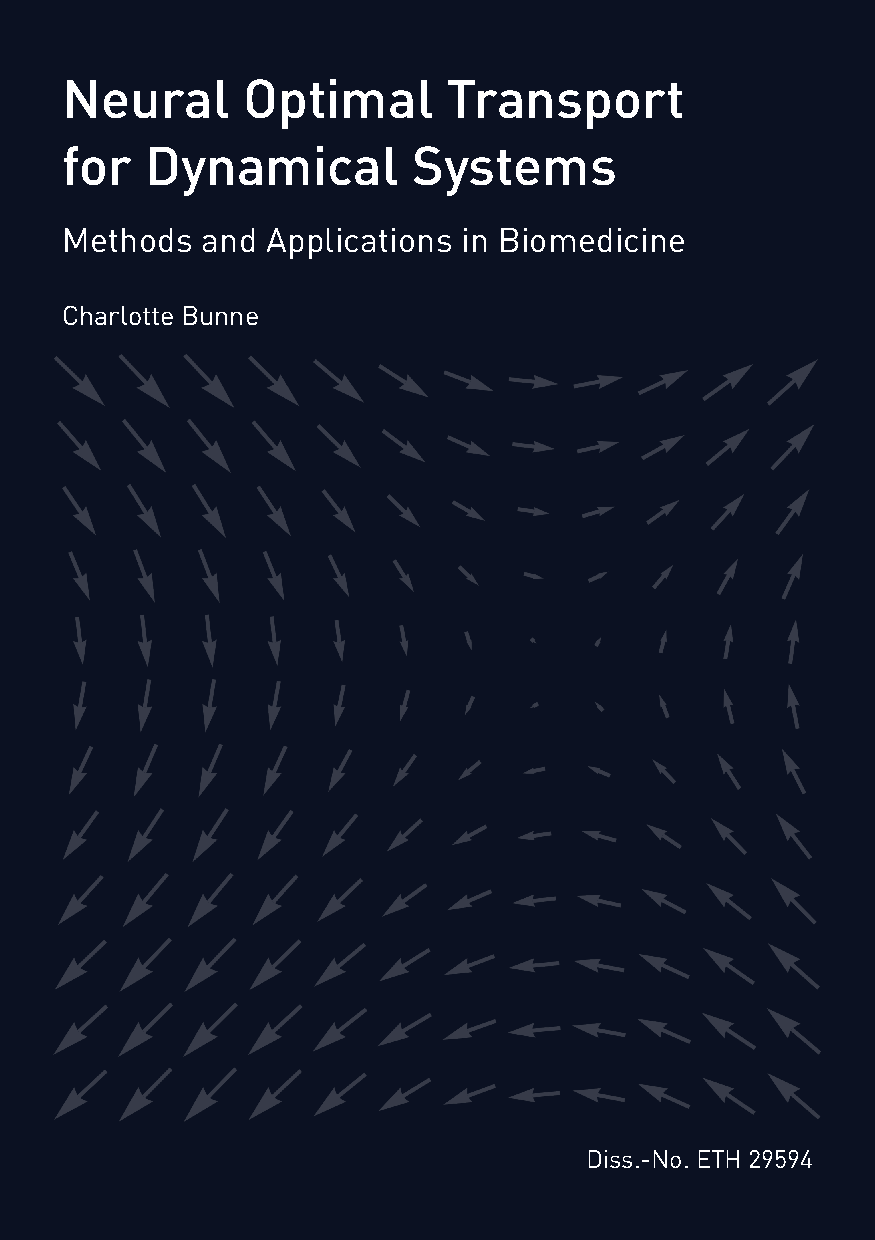
\includepdf[pages={1,{}}]{cover/crop/cover_tmp.pdf}
\cleardoublepage\setcounter{page}{1}

% Frontmatter
%*******************************************************
% Little Dirty Titlepage
%*******************************************************
\thispagestyle{empty}
%*******************************************************
\begin{center}
    \spacedlowsmallcaps{\myName} \\ \bigskip                        

    \begingroup
        \color{chaptercolor}\spacedallcaps{\large \myTitle}\\
        \vspace{5pt}\spacedallcaps{\footnotesize \mySubtitle}
    \endgroup
\end{center}        

%*******************************************************
% Titlepage
%*******************************************************
\begin{titlepage}
	% if you want the titlepage to be centered, uncomment and fine-tune the line below (KOMA classes environment)
	%\begin{addmargin}[-1cm]{-3cm}
    \begin{center}
        \large
        \begingroup
            \spacedlowsmallcaps{Diss. ETH No. \myDissNumber}
        \endgroup

        \hfill

        \vfill

        \begingroup
            \spacedallcaps{\myTitle}\\
            \vspace{5pt}\spacedallcaps{\footnotesize \mySubtitle}\\
            %\spacedallcaps{\myTitleLineTwo}\\
            %\spacedallcaps{\myTitleLineThree}
        \endgroup

        \vfill

        \begingroup
            A thesis submitted to attain the degree of\\
            \vspace{0.5em}
            \spacedlowsmallcaps{Doctor of Sciences} \\
            (Dr.\ sc.\ ETH Zurich)
        \endgroup

        \vfill

        \begingroup
            presented by\\
            \vspace{0.5em}
            \spacedallcaps{\normalsize \myName} \\
            M.\ sc.\ ETH Zurich \\
            \vspace{0.5em}
            born on 29 August 1995\\
            % citizen of Germany
        \endgroup

        \vfill

        \begingroup
            accepted on the recommendation of\\
            \vspace{0.5em}
            Prof.\ Dr.\ Andreas Krause, examiner \\
            Prof.\ Dr.\ Marco Cuturi, co-examiner \\
            Prof.\ Dr.\ Lucas Pelkmans, co-examiner \\
            Prof.\ Dr.\ Jure Leskovec, co-examiner \\
        \endgroup

        \vfill

        \myTime%

        \vfill
    \end{center}
  %\end{addmargin}
\end{titlepage}

\thispagestyle{empty}

\hfill

\vfill

\noindent\myName: \textit{\myPlainTitle,} %\mySubtitle, %\myDegree, 
\textcopyright\ \myTime

%\bigskip

%\noindent\spacedlowsmallcaps{DOI}: \myDOI

% \bigskip

% \noindent\spacedlowsmallcaps{Supervisors}: \\
% \myProf \\
% \myOtherProf \\ 
% \mySupervisor

% \medskip

% \noindent\spacedlowsmallcaps{Location}: \\
% \myLocation

% \medskip

% \noindent\spacedlowsmallcaps{Time Frame}: \\
% \myTime

\cleardoublepage%*******************************************************
% Dedication
%*******************************************************
\thispagestyle{empty}
%\phantomsection
\refstepcounter{dummy}
%\pdfbookmark[1]{Dedication}{Dedication}

\vspace*{3cm}

\dictum[Johann Wolfgang von Goethe, \textit{Faust I} (1808)]{%
  Und was in schwankender Erscheinung schwebt, \\
  Befestiget mit dauernden Gedanken.}
\cleardoublepage%*******************************************************
% Abstract
%*******************************************************
%\renewcommand{\abstractname}{Abstract}
\pdfbookmark[1]{Abstract}{Abstract}
\begingroup
\let\clearpage\relax
\let\cleardoublepage\relax
\let\cleardoublepage\relax

\chapter*{Abstract}

Modeling dynamical systems is a core subject of many scientific disciplines as it allows us to predict future states, understand complex interactions over time, and enable informed decision-making.
Biological systems in particular are governed by dynamical processes, with their inherently complex and constantly changing patterns of interactions and behaviors.
Single-cell biology thereby has revolutionized biomedical research, as it allows to monitor such systems at unprecedented scales.
At the same time, it presents us with formidable challenges: While single-cell high-throughput methods routinely produce millions of data points, they are destructive assays, such that the same cell cannot be observed twice nor profiled over time.
Since many of the most pressing questions in the field involve modeling the dynamic responses of heterogeneous cell populations to various stimuli, such as therapeutic drugs or developmental signals, there is a pressing need to provide computational methods that can circumvent that limitation and re-align these unpaired measurements.

Optimal transport (OT) has emerged as a major opportunity to fill in that gap \textit{in silico} as it allows us to reconstruct how a distribution evolves, given only access to \emph{distinct snapshots} of \emph{unaligned} data points.
Classical OT methods, however, do not generalize to \emph{unseen} samples. Yet, this is crucial when, for example, predicting treatment responses of incoming patient samples or extrapolating cellular dynamics beyond the measured horizon.

By harnessing the theoretical constructs of OT, this thesis explores and develops \textbf{\emph{neural}} \textbf{static} and \textbf{dynamic optimal transport} schemes for elucidating the intricate dynamics of biological populations. It encapsulates an array of algorithmic frameworks, with contributions to both the \textit{understanding} and \textit{prediction} of population dynamics:

\begin{itemize}[leftmargin=*]
	\item First, we derive \textbf{static neural optimal transport} schemes capable of learning a map between the unpaired distributions of unperturbed and perturbed cells. These models excel at predicting single-cell responses to varying perturbations, such as cancer drug screens, and generalize the inference of treatment outcomes to \emph{unobserved} cell types and patients.
This has significant implications for personalized medicine, as it allows for the prediction of treatment responses for new patients in large-scale clinical studies.

	\item Second, we explore \textbf{dynamic neural optimal transport} formulations that leverage the connections of OT to partial differential equations and gradient flows through the \acrfull{JKO} scheme, as well as stochastic differential equations and optimal control through diffusion Schr{\"o}dinger bridges. These methods then serve as robust tools for reconstructing stochastic and continuous-time dynamics from marginal observations, allowing us to dissect fine-grained and time-resolved cellular mechanisms.
\end{itemize}

This thesis connects a variety of seemingly unrelated concepts into a unified framework, and the presented methodologies offer a computational and mathematical foundation for modeling of cellular dynamics. This provides new avenues to understand cellular heterogeneity, plasticity, and response landscapes.
By providing neural parameterizations of static and dynamic OT that allow for out-of-sample inference, the developed methods anticipate broad implications, spanning from understanding developmental trajectories to predicting patient-specific drug responses and designing personalized therapies.

% Cell populations are almost always heterogeneous in function and fate. To understand the plasticity of cells and their responses to molecular perturbations, such as drugs or developmental signals, it is vital to recover the underlying population dynamics and fate decisions of single cells. However, measuring features of single cells requires destroying them. As a result, a cell population can only be monitored with sequential snapshots, obtained by sampling a few particles that are sacrificed in exchange for measurements.

% This celebrated theory provides the mathematical link that unifies the several contributions to model cellular dynamics that we present here: 
\endgroup

\cleardoublepage%

\begingroup
\let\clearpage\relax
\let\cleardoublepage\relax
\let\cleardoublepage\relax

\begin{otherlanguage}{ngerman}
\pdfbookmark[1]{Zusammenfassung}{Zusammenfassung}
\chapter*{Zusammenfassung}

Die Modellierung dynamischer Systeme bildet einen Schwerpunkt in vielen wissenschaftlichen Fachbereichen. Sie erm{\"o}glicht es uns, zuk{\"u}nftige Zust{\"a}nde vorherzusagen, komplexe zeitliche Interaktionen zu analysieren und fundierte Entscheidungen zu treffen. Insbesondere in biologischen Systemen, die von inh{\"a}rent komplexen und st{\"a}ndig wechselnden Interaktions- und Verhaltensmustern gesteuert werden, kommt dieser Aspekt zum Tragen.
Die Einzelzellbiologie hat dabei biomedizinische Forschung revolutioniert, indem sie es erm{\"o}glicht, solche Systeme in beispielloser Gr{\"o}{\ss}enordnung zu messen. Gleichzeitig stellt sie uns vor gewaltige Herausforderungen: Obwohl Einzelzell-Hochdurchsatzmethoden routinem{\"a}{\ss}ig Millionen von Datenpunkten produzieren, sind es destruktive Assays, sodass dieselbe Zelle nicht wiederholt oder kontinuierlich {\"u}ber die Zeit gemessen werden kann.
Angesichts dringender Fragen zur Modellierung der dynamischen Reaktionen heterogener Zellpopulationen auf verschiedene Perturbationen, wie therapeutische Medikamente oder Entwicklungssignale, besteht ein akuter Bedarf an der Entwicklung von Algorithmen, die diese Einschr{\"a}nkung {\"u}berwinden und zeitliche Trajektorien einzelner Zellen rekonstruieren k{\"o}nnen.

Die mathematische Theorie des sogenannten optimalen Transports (OT) hat sich dabei als Schl{\"u}sselmethodik etabliert, um diese L{\"u}cke \emph{in silico} zu schlie{\ss}en. OT erlaubt es uns zu rekonstruieren, wie sich eine Verteilung {\"u}ber die Zeit hinweg entwickelt hat, selbst aus \textit{diskreten Messungen} von \textit{nicht gekoppelten Datenpunkten}. Allerdings generalisieren klassische OT Methoden nicht auf unbekannte Proben, eine entscheidende F{\"a}higkeit f{\"u}r die Vorhersage von Behandlungsreaktionen oder wenn zellul{\"a}re Dynamiken {\"u}ber den gemessenen Horizont hinaus extrapoliert werden sollen.

Diese Dissertation entwickelt, basierend auf den theoretischen Konzepten des optimalen Transports, sowohl \textbf{\textit{neuronale} statische} als auch \textbf{dynamische optimale Transport} Systeme, um die komplexen Dynamiken biologischer Populationen zu modellieren und zu verstehen:

\begin{itemize}[leftmargin=*]
	\item \textbf{Statischer neuronaler optimaler Transport}: 
	Diese Methoden sind in der Lage, eine Abbildung zwischen ungepaarten Verteilungen von unperturbierten und perturbierten Zellen zu erlernen. Sie erziehlen sehr gute Ergebnisse in der Vorhersage von Einzelzellreaktionen auf verschiedene Perturbationen, wie zum Beispiel Krebsmedikamenten, und erm{\"o}glichen die Vorhersage von Behandlungsreaktionen f{\"u}r neue Patienten in gro{\ss} angelegten klinischen Studien.

	\item \textbf{Dynamischer neuronaler optimaler Transport}: 
	Durch das Verkn{\"u}pfen von OT zu partiellen Differentialgleichungen und Gradientenfl{\"u}ssen durch das \acrfull{JKO} Schema, sowie stochastischer Differentialgleichungen und optimalen Steuerungen durch Diffusion Schr{\"o}dinger Br{\"u}cken dienen diese Algorithmen als robuste Werkzeuge zur Rekonstruktion stochastischer und kontinuierlicher Zeitdynamiken. Sie erm{\"o}glichen dadurch feink{\"o}rnige Analysen zeitlich aufgel{\"o}ster zellul{\"a}rer Mechanismen.
\end{itemize}

Diese Dissertation verbindet eine Vielzahl scheinbar nicht verwandter Konzepte in einem einheitlichen Rahmen und bietet eine methodische und mathematische Grundlage f{\"u}r die Modellierung zellul{\"a}rer Dynamiken. 
Sie ebnet neue Wege, zellul{\"a}re Heterogenit{\"a}t, Plastizit{\"a}t und Reaktionen zu Perturbationen zu erforschen. Die entwickelten neuronalen Parameterisierungen von statischem und dynamischem OT, die eine au{\ss}erhalb der Stichprobe liegende Inferenz erm{\"o}glichen, haben weitreichende Auswirkungen, von dem Verstehen entwicklungsbiologischer Prozesse bis hin zur Vorhersage von patientenspezifischen Medikamentenreaktionen und der Gestaltung personalisierter Therapien.

% Die Modellierung dynamischer Systeme ist ein Kernthema vieler wissenschaftlicher Disziplinen, da es uns erm{\"o}glicht, zuk{\"u}nftige Zust{\"a}nde vorherzusagen, komplexe zeitliche Interaktionen zu verstehen und informierte Entscheidungen zu treffen.
% Biologische Systeme werden insbesondere durch dynamische Prozesse gesteuert, mit ihren inh{\"a}rent komplexen und st{\"a}ndig wechselnden Mustern von Interaktionen und Verhaltensweisen.
% Einzelzellbiologie hat dabei die biomedizinische Forschung revolutioniert, da sie es erm{\"o}glicht, solche Systeme in beispielloser Gr{\"o}{\ss}e zu {\"u}berwachen.
% Gleichzeitig stellt sie uns vor gewaltige Herausforderungen: W{\"a}hrend Einzelzell-Hochdurchsatzmethoden routinem{\"a}{\ss}ig Millionen von Datenpunkten produzieren, handelt es sich um destruktive Assays, so dass dieselbe Zelle nicht zweimal beobachtet oder als kontinuierlich Zeitreihe gemessen werden kann.
% Da viele der dr{\"a}ngendsten Fragen auf dem Gebiet die Modellierung der dynamischen Reaktionen heterogener Zellpopulationen auf verschiedene Perturbationen, wie therapeutische Medikamente oder Entwicklungssignale, betreffen, besteht ein dringender Bedarf, Algorithmen zu entwickeln, die diese Einschr{\"a}nkung umgehen und zeitliche Trajektorien einzelner Zellen rekonstruieren k{\"o}nnen.

% Optimaler Transport (OT) hat sich als kritische Methodik herauskristallisier, um diese L{\"u}cke \textit{in silico} zu schlie{\ss}en. OT erm{\"o}glicht es uns aus \emph{diskreten Messungen} von \emph{nicht gekoppelten} Datenpunkten zu rekonstruieren, wie eine Verteilung sich {\"u}ber die Zeit hin entwickelt hat.
% Klassische OT-Methoden generalisieren jedoch nicht auf \emph{unbekannte} Proben. Dies ist jedoch entscheidend, wenn beispielsweise die Behandlungsreaktionen von eingehenden Patientenzellen vorhergesagt oder die zellul{\"a}ren Dynamiken {\"u}ber den gemessenen Horizont hinaus extrapoliert werden sollen.

% Basierend auf den theoretischen Konstrukten von OT entwickelt diese Dissertation \textbf{\emph{neuronale} statische} und \textbf{dynamische optimale Transport} Systeme um komplexen Dynamiken biologischer Populationen zu modellieren und verstehen. Sie umfasst eine Reihe von algorithmischen Rahmenkonzepten, mit Beitr{\"a}gen sowohl zum \textit{Verst{\"a}ndnis} als auch zur \textit{Vorhersage} der Populationsdynamik:

% Zun{\"a}chst entwickeln wir \emph{statische neuronale optimale Transport} Schemata, die in der Lage sind, eine Abbildung zwischen den ungepaarten Verteilungen von unperturbierten und perturbierten Zellen zu erlernen. Diese Modelle sind ausgezeichnet in der Vorhersage von Einzelzellreaktionen auf verschiedene St{\"o}rungen, wie Krebsmedikamententests, und verallgemeinern die Ableitung von Behandlungsergebnissen auf \emph{unbeobachtete} Zelltypen und Patienten.
% Dies hat erhebliche Auswirkungen auf die personalisierte Medizin, da es die Vorhersage von Behandlungsreaktionen f{\"u}r neue Patienten in gro{\ss} angelegten klinischen Studien erm{\"o}glicht.

% Zweitens erforschen wir \emph{dynamische neuronale optimale Transport} Formulierungen, die die Verbindungen von OT zu partiellen Differentialgleichungen und Gradientenfl{\"u}ssen durch das \acrfull{JKO} Schema, sowie stochastische Differentialgleichungen und optimale Kontrolle durch Diffusion Schr{\"o}dinger Br{\"u}cken nutzen. Diese Methoden dienen dann als robuste Werkzeuge zur Rekonstruktion stochastischer und kontinuierlicher Zeitdynamiken aus Randbeobachtungen und erm{\"o}glichen es uns, feink{\"o}rnige und zeitlich aufgel{\"o}ste zellul{\"a}re Mechanismen zu analysieren.

% Diese Arbeit verbindet eine Vielzahl scheinbar nicht verwandter Konzepte zu einem einheitlichen Rahmen, und die vorgestellten Methoden bieten eine methodische und mathematische Grundlage f{\"u}r die Modellierung zellul{\"a}rer Dynamik. Dies bietet neue Wege, zellul{\"a}re Heterogenit{\"a}t, Plastizit{\"a}t und Antwortlandschaften zu verstehen.
% Indem neuronale Parameterisierungen von statischem und dynamischem OT entwickelt werden, die eine au{\ss}erhalb der Stichprobe liegende Inferenz erm{\"o}glichen, erwarten die entwickelten Methoden weitreichende Auswirkungen, die von der Verst{\"a}ndigung von Entwicklungsverl{\"a}ufen bis zur Vorhersage von patientenspezifischen Medikamentenreaktionen und der Gestaltung personalisierter Krebstherapien reichen.

\end{otherlanguage}

\endgroup

\vfill
\cleardoublepage%*******************************************************
% Acknowledgments
%*******************************************************
\pdfbookmark[1]{Acknowledgements}{acknowledgements}

\bigskip

\begingroup
\let\clearpage\relax
\let\cleardoublepage\relax
\let\cleardoublepage\relax
\chapter*{Acknowledgements}

\def\thanks#1{%
\begingroup
\leftskip1em
\noindent #1
\par
\endgroup
}

First and foremost, I would like to express my sincere gratitude to my advisor Andreas Krause for his excellent mentorship, continued support, for innovative ideas, precise remarks, and critical thinking.
Thank you in particular for your trust and for finding the right balance between guidance and giving me the freedom to pursue my research interests.
Your remarkable insights into which ideas are likely to succeed as well as how to communicate a scientific result never cease to amaze me and will remain with me as a particularly valuable lesson for the future.

I would like to extend my gratitude to Marco Cuturi for being my co-advisor from the very beginning. 
Without your invaluable mentorship, this thesis would certainly not be the same. Thank you for empowering me to acquire novel skills and develop and realize my own research agenda.
Also, thank you for providing me with countless opportunities ranging from internships at Google Research and Apple to co-presenting the tutorial at ICML 2023 with me. \\
This combination of advisors has been key for my doctorate studies. \\

Further, I would also like to thank Jure Leskovec for participating in my thesis committee and for providing me with insightful feedback. 
Throughout my academic path, various scientists have left a mark on me as a researcher, chief among them Aviv Regev. While our academic collaboration is still at the very beginning, every interaction with you is intellectually rewarding.
I am excited about the upcoming chapter with both of you at Stanford and Genentech.

\looseness -1 The thesis would not be the same without the longstanding collaboration with Lucas Pelkmans and Gabriele Gut. First, thank you, Lucas, for serving on my thesis committee.
I have particularly enjoyed our academic ventures at the intersection  of molecular biology and machine learning. Working with you has taught me to think differently about problems, ask different questions, and had a lasting effect on this thesis.

I am very grateful to Anne Carpenter and Shantanu Singh for hosting me at the Broad Institute of MIT and Harvard and for the many research discussions we had. I will forever cherish my time in your lab.

I am profoundly indebted to all co-authors and fantastic collaborators with whom I worked on many projects throughout the past years, in particular, Gunnar R\"atsch, Stefan Stark, Ya-Ping Hsieh,  Matteo Pariset, Valentin De Bortoli, Octavian Ganea, Vignesh Ram Somnath, Frederike L{\"u}beck, Laetitia Meng-Papaxanthos, Mojm{\'i}r Mutn{\'y}, Regina Barzilay, Tommi Jaakkola, Connor Coley, and Philippe Schwaller. Thank you especially to Ya-Ping Hsieh and Stefan Stark for hour-long discussions on various projects. 

Further, I am very grateful to my first academic mentors, Stefanie Jegelka, David Alvarez Melis, Roland Eils, Thomas H{\"o}fer, and Lisa Buchauer for guiding me through my first actual research projects.
Thank you, Stefanie, for being a mentor much beyond my time at MIT and for your continued advice. 
Thank you, David, for introducing me to optimal transport many years back, for every coffee during the frequent visits to Cambridge, and in particular, for navigating me through my faculty search and life in academia. I learned so much from you and will be forever grateful.

Lastly, I would not have started my scientific journey without the Life-Science Lab at the German Cancer Research Center. It is what sparked my interest in biology and engineering and set the course for what is here today.
Participating in the "world championship in synthetic biology" was an eye-opener for the power and potential of interdisciplinary research.

\looseness -1 Thanks to all members of the Learning and Adaptive Systems group at ETH Zurich and the ETH AI Center for creating an excellent research environment. Thanks to Lars Lorch, Mohammad Reza Karimi, and Lenart Treven for lengthy discussions on causal inference, sampling, or control theory. 
Thank you, Rita Klute, for the support, for entangling the jungle of bureaucracy, and for overcoming \emph{any} administrative hurdle. \\

I am very grateful to my parents Nele and Egon and my siblings Kaspar, Henriette, and Frieder for their endless love, advice, encouragement, and support.
Growing up in this environment of Freigeister has made me the person I am today.

Thank you to my friends around the globe for making life joyful and adventurous, every party fun, and the difficult moments bearable.

Lastly, thank you to Pol for expanding my world into unknown dimensions: "Jeder Zustand, ja jeder Augenblick [mit dir] ist von unendlichem Wert, denn er ist der Repr{\"a}sentant einer ganzen Ewigkeit."\footnote{Johann Peter Eckermann and Johann Wolfgang von Goethe. Gespr{\"a}che mit Goethe in den letzten Jahren seines Lebens. 1823-1832: 2. Vol. 2. FA Brockhaus, 1836.}


\endgroup

\pagestyle{scrheadings}
\cleardoublepage\null

% Table of Contents
\refstepcounter{dummy}
\pdfbookmark[1]{\contentsname}{tableofcontents}
\setcounter{tocdepth}{2} % <-- 2 includes up to subsections in the ToC
\setcounter{secnumdepth}{3} % <-- 3 numbers up to subsubsections
\manualmark%
\markboth{\spacedlowsmallcaps{\contentsname}}{\spacedlowsmallcaps{\contentsname}}
\tableofcontents
\automark[section]{chapter}
\renewcommand{\chaptermark}[1]{\markboth{\spacedlowsmallcaps{#1}}{\spacedlowsmallcaps{#1}}}
\renewcommand{\sectionmark}[1]{\markright{\thesection\enspace\spacedlowsmallcaps{#1}}}

% Notation and Acronyms
\begingroup

\refstepcounter{dummy}
\pdfbookmark[1]{Notation}{notation}
\markboth{\spacedlowsmallcaps{Notation}}{\spacedlowsmallcaps{Notation}}
\chapter*{Notation}

\let\clearpage\relax
\let\cleardoublepage\relavx
\let\cleardoublepage\relax

\vskip -2em
\begin{tabularx}{\textwidth}{lX}
 	$\Sigma_n$ & probability simplex of size $n$. \\
 	$(\mu, \nu)$ & measures defined on spaces $(\gX, \gY)$. \\
 	$(u, v)$ & histograms in the simplices $\Sigma_n \times \Sigma_m$. \\
 	$p_\mu = \frac{d\mu}{dx}$ & density with respect to the Lebesgues measure. \\
 	\makecell{$(\mu=\sum_i u_i \delta_{x_i},$ \\ $\,\nu=\sum_j v_j \delta_{y_j})$} & discrete measures defined on spaces $(x_1, \dots, x_n \in \gX, y_1, \dots, y_m \in \gY)$. \\
 	$\mathbf{1}$ & matrix of $\mathbb{R}^{n \times m}$ with all entries identically set to 1. \\
 	$\mathds{1}$ & indicator function. \\
 	$c(x, y)$ & ground cost, with associated pairwise cost matrix $(c(x_i,y_j))_{ij}$ evaluated on the support of $\mu, \nu$. \\
 	$\sharp$ & pushforward operator. \\
 	$T: \gX \times \gY$ & Monge map, typically such that $T_\sharp \mu = \nu$. \\
 	$\pi$ & coupling measure between $\mu$ and $\nu$, for discrete measures $\pi = \sum_{ij} \mathbf{P}_{ij} \delta_{(x_i, y_j)}$. \\
 	$\Pi(\mu, \nu)$ & set of couplings, for discrete measures $U(u, v)$. \\
 	$\supp(\pi)$ & support of $\pi$. \\
 	$(\mu_t)_{t=0}^T$ & dynamic measures with $\mu_{t=0} = \mu_0$ and $\mu_{t=T} = \mu_T$. \\
 	$(f, g)$ & dual potentials. \\
 	$v$ & speed in the dynamic Benamou-Brenier or control in the stochastic optimal control formulation. \\
 	$\Delta$ & Laplace operator. \\
 	
\end{tabularx}

\printacronyms
\endgroup

\clearpage
\cleardoublepage\null

% Mainmatter
\cleardoublepage%
\pagenumbering{arabic}%
\chapter{Introduction}
\label{cha:introduction}

\dictum[Rachel Carson, \textit{Silent Spring} (1962)]{%
  The balance of nature is not a status quo; it is fluid, ever shifting, in a constant state of adjustment. \\ Man, too, is part of this balance.}%
\vskip 2em

Dynamical systems are governing every aspect of life, encapsulating the unifying principles and complex interactions that shape our world. They are the cornerstone of diverse scientific fields such as physics, chemistry, and biology. In physics, they assist in understanding the movement and interaction of objects large and small, from planetary orbits to particle motion.
In the world of chemistry, they guide the interaction and transformation of molecules, offering insights into reaction dynamics and molecular behavior.
In biology it opens doors to insights ranging from the dynamic signaling activities in single cells to the ebb and flow of entire ecosystems.

Given the complexity and constant evolution inherent in living organisms, the application of dynamical systems in biology offers a particularly rich and challenging field of study.
Biology is determined by structure, patterns, and dynamics at various scales, ranging from molecular interactions to organismal behavior.
% Recent technologies have provided access, with an unprecedented resolution, once deemed unthinkable, into the inner workings of cells and tissues that lie on the lower-end of that scale.
At the lower end of that scale, advances in \acrlong{sc} genomics and transcriptomics provide now a direct window, with a resolution that was deemed unthinkable two decades ago, into the molecular makeup of individual cells, capturing vividly the inner workings of cells at any point in time.
% paving the way for a better understanding of the diversity of cell types and their functional roles. 
Similarly, advances in imaging technology provide tools to map the spatial organization of tissues and organs at the cellular and subcellular level, improving our understanding of key physiological processes that underlie health and disease. \\

The ability of single-cell high-throughput methods to produce routinely millions of data points holds multiple promises. They do, however, come with several limitations: 
 Most prominently, they are typically destructive assays as cells are usually fixed and stained or chemically destroyed to obtain measurements. Thus, they produce data points that are not \textit{aligned}, meaning that the same cell cannot be observed twice nor can we record continuous time trajectories of it.
Since many of the most pressing questions in the field involve modeling and understanding the dynamic responses of heterogeneous cell populations to various stimuli, such as environmental signals, developmental processes, genetic perturbations, or drug treatments, there is a pressing need to provide algorithms that can circumvent that limitation and (\colcircle{lightblue}) \textbf{reconstruct such dynamical processes}. 
This constraint is particularly acute in the field of personalized medicine, where the goal is precisely to understand the dynamic response of a patient's cells to a stimulus, and would therefore rest, in theory, on the ability to observe the same cell before and after treatment. \\

Significantly, the diversity within a cell population, or \textit{cellular heterogeneity}, plays a crucial role in determining how sensitive or resistant cells are to perturbations.
Rather than resorting to population averages, we need to (\colcircle{pink}) \textbf{model the problem at the particle level}, e.g., based on distributions of single cells, in order to capture and then further analyze the distinct cells' responses to a perturbation. 
This requires scalable and principled algorithms that are well aligned with the constrained experimental settings of high-throughput methods and incorporate the inherent structure of biological processes. \\

Beyond, to effectively derive complex and nonlinear dynamic processes from data, it is essential to (\colcircle{blue}) \textbf{develop neural network-based parameterizations} of such processes.
Traditional mathematical models might not be sufficient to capture all intricacies of a system. This holds particularly true in biology, where our understanding of the underlying mechanisms is incomplete and many factors contribute to the overall dynamics.
Most importantly, \acrfullpl{NN} allow us to infer and forecast dynamical processes. This enables \emph{out-of-sample} predictions of the evolution of previously unseen particles, such as unobserved cells from incoming patient samples and to extrapolate the inference to new cell types or beyond the recorded time horizon. \\

However, despite recent successes of deep learning in many areas such as computer vision \citep{lecun1998gradient, krizhevsky2012imagenet}, natural language processing \citep{bengio2000neural, vaswani2017attention}, game playing \citep{mnih2015human, silver2016mastering}, and biochemistry \citep{jumper2021highly, kipf2016semi, jin2021iterative}, deep neural networks still fall short of a general ability to model dynamic and complex evolutions of populations of particles.
At the heart of this challenge lies the problem of inductive bias \citep{mitchell1980need}: How can models be constructed to learn the essential representations, abstractions, and skills that will enable them to generalize to unseen and unforeseeable situations?

The examples above highlight the effectiveness of crafting specific architectural inductive biases that are tailored to the object of study: \acrfullpl{CNN} in computer vision contain filters that process local features in an image, \acrfullpl{RNN} with attention layers in natural language processing facilitate the comprehension of long-range connections in sentences, or \acrfullpl{GNN} account for neighborhood structures to simulate chemical interactions within proteins and molecules \citep{ganea2021geomol, somnath2021multi}.
Introducing and developing (\colcircle{darkblue}) \textbf{inductive biases in deep learning architectures for population dynamics}  is quintessential toward the success and ability of such methods to capture complex dynamics from \emph{unaligned} snapshot data.


\section{Scope and Contributions}

In this thesis, we introduce and design novel deep learning architectures capable of modeling heterogeneous population dynamics from unaligned snapshot data.
A framework that facilitates the design of such deep learning architectures that (\colcircle{pink}) operate on distributions, i.e., allows modeling heterogeneous populations of particles, (\colcircle{lightblue}) trained based on samples of \emph{unaligned} distributions is the \textbf{theory of optimal transport}.

The mathematical foundation of this work further builds on the intuition that perturbations incrementally alter the molecular profiles of cells. This underlying assumption aligns with the theory of \acrfull{OT} that studies the evolution of measures under the \emph{minimum effort} principle. Thus, (\colcircle{darkblue}) OT serves naturally as an inductive bias for the deep learning architectures introduced in this thesis.
By providing tools for modeling the evolution of distributions over time, OT allows us to reconstruct and predict the incremental changes in cell states upon perturbation such as therapeutic agents or developmental signals. 
In recent years, OT has enabled significant advances in single-cell biology problems \citep{schiebinger2019optimal, lavenant2021towards, demetci2022scot}. However, traditional OT methods do not enable predictions for unperturbed cells that have not been previously observed.
They are thus unable to predict perturbation responses out-of-sample, e.g., of cells from new incoming samples, such as those from unseen patients. 
This thesis is thus concerned with the development of so-called  (\colcircle{blue}) \textbf{neural optimal transport} methods that allow for out-of-sample \emph{predictions} on unseen cells and \emph{forecasting} of cellular dynamics \citep{makkuva2020optimal, tong2020trajectorynet,  korotin2021wasserstein, bunne2022proximal, bunne2022supervised, bunne2021learning}. \\

\begin{figure}[t]
  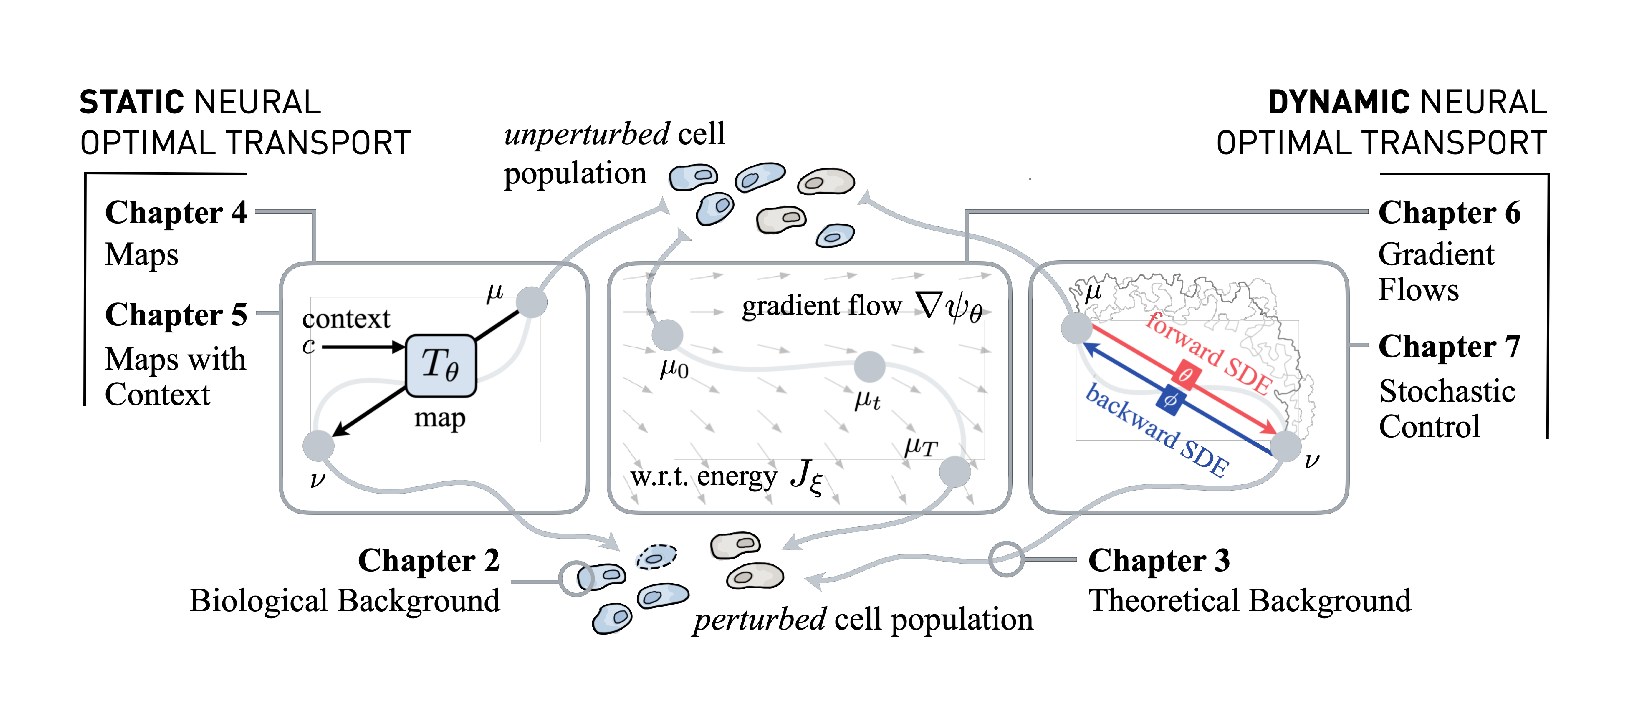
\includegraphics[width=\textwidth]{figures/fig_overview_thesis.pdf}
  \caption{Structure of the thesis with references to the chapters.}
  \label{fig:overview_thesis}
\end{figure}

Optimal transport comes in many different flavors and has strong mathematical roots in dynamical systems theory:

The goal of the \emph{static} formulation of OT is to identify a map that \emph{optimally} morphs or transports a distribution onto another, and thus "best" explains the one-step evolution of a measure.
The static framework, however, has an immediate dynamic interpretation. By introducing a time-variable into the transport, OT allows us to study the continuous evolution of a measure over time. % , critical when aiming at interpolating between different measurements.
Importantly, generalizations of this \emph{dynamic} formulation can be formalized through ordinary, partial, or stochastic differential equations: By building on innovations in neural \acrfullpl{ODE} \citep{chen2018neural} and flow matching models \citep{lipman2023flow, pooladian2023multisample, liu2022flow}, physics-informed neural \acrfullpl{PDE} \citep{brandstetter2022message, raissi2019physics}, as well as \acrfullpl{SDE}-based neural network frameworks of \acrfullpl{SGM}, neural OT methods can be equipped with various powerful backbone architectures.

The thesis is structured as follows (see outline in \cref{fig:overview_thesis}).
After reviewing dynamical systems in biomedicine in \cref{cha:bio_background} and providing a mathematical foundation of static and dynamic optimal transport in \cref{cha:theory_background}, the \textbf{thesis contributions} are then organized in two parts:

\paragraph{\cref{part:static_not}: Static neural optimal transport.}

At its core, static OT defines a so-called \citeauthor{monge1781histoire} \textit{map}, which provides an actionable way to flow from one probability distribution onto another.
The design of neural network-parameterizations of such maps and their application to predict perturbation responses of single-cells will form the first contribution of this thesis.
This comprises approaches that are a direct consequence of the famous \citeauthor{brenier1987decomposition} theorem, and allow us to model Monge maps as gradients of convex functions \citep{bunne2021learning, bunne2022supervised}.

More concretely, \cref{part:static_not} comprises two chapters:
\cref{cha:cellot} proposes \textsc{CellOT}, a framework leveraging optimal transport theory and convex neural architectures that aligns unpaired distributions of unperturbed and perturbed cells to predict individual cellular responses to various perturbations. 
\textsc{CellOT} outperforms current methods in drug response predictions, and provides ways for interpretation and understanding of heterogeneous single-cell responses and patient-specific treatment outcomes \citep{bunne2021learning}. 

Further, \cref{cha:condot} generalizes the above framework and introduces the \textsc{CondOT} model, a multi-task approach that parameterizes a \emph{family of OT maps} that can be conditioned on a context variable. Conditioning thereby allows, for example, to predict the response of single-cells to combination therapies, i.e., the inference of the effect of genetic or therapeutic perturbations applied in combination \citep{bunne2022supervised}. \\
	
% \textbf{Applications:} Predicting responses of heterogeneous cell populations to molecular perturbations (e.g., genetic knockouts or overexpression, chemical drugs, or developmental signals) at the level of single cells
% A fundamental difficulty is thus to reconstruct perturbation responses of individual cells from a set of unaligned unperturbed and perturbed cells. To forecast patient cell reactions to treatments or deduce cell differentiation paths, we need to reconcile these unpaired snapshots, thus predicting each cell's perturbed state.


\paragraph{\cref{part:dynamic_not}: Dynamic neural optimal transport.}

Beyond mappings, OT provides a mathematical link to geometric variational frameworks that allow studying flows of distributions on metric spaces.
In particular, \citeauthor{brenier1987decomposition}'s dynamical formulation of OT has given rise to a flurry of applications studying \acrshortpl{PDE} as gradient flows or steepest descent in spaces of probability measures.
% \citet*{benamou2000computational} demonstrate how the dynamic point of view offers an alternate and intuitive interpretation of optimal transport with links to fluid dynamics that surprisingly leads to a convex optimization problem that can be parameterized through normalizing flows \citep{tong2020trajectorynet}.
This thesis highlights the connections of OT to PDEs such as Fokker-Planck-like equations through the \citeauthor*{jordan1998variational} scheme: In recent works \citep{bunne2022proximal, alvarez2021optimizing, mokrov2021large, benamou2016augmented} 
it has found application in inferring the evolution of populations over time, crucial in many scientific disciplines when for instance, observing a population of cells in biology.

\cref{cha:neural_pde} thereby introduces a reformulation of the JKO objective that allows for gradient-based learning in an end-to-end fashion. Further, it proposes \textsc{JKOnet}, a neural network architecture that models the collective dynamics of particle populations by learning the causal JKO flow from measurement snapshots, trading off energy improvements with closeness to previous configurations, and demonstrating robust performance \citep{bunne2022proximal}.

Lastly, beyond PDEs, this thesis explores the relation between the optimal transport problem and the \acrfull{SB} problem from stochastic control. It represents a key connection that has recently fueled the development of \acrfull{DSB} \citep{de2021diffusion, chen2021stochastic, liu2022deep, bunne2022recovering}. Estimating such bridges, however, is notoriously difficult, motivating our contributions in \cref{cha:neural_sde} for novel adaptive schemes:

First, in \cref{sec:gsbflow} our goal is to rely on Gaussian approximations of the data to provide the reference stochastic process needed to estimate \acrshortpl{SB}. To that end, we solve the \acrlong{SB} problem with Gaussian marginals, for which we derive, as a central contribution, a closed-form solution and SDE-representation. We use these formulas to define the reference process used to estimate more complex \acrshortpl{SB}, and show that this does indeed help with its numerical solution of learning \acrlongpl{DSB}. We obtain notable improvements when reconstructing single-cell genomics experiments of developmental embryoid body diffierentiation \citep{bunne2022recovering}.

Second, parallel developments in bioengineering aim at circumventing the destructive nature of high-throughput methods and provide us with methodology that allows for partial tracking of single-cell trajectories over time.
In \cref{sec:sbalign}, we thus introduce a novel algorithmic framework for solving \acrlongpl{DSB} that respects data alignment and incorporates \emph{sparse} trajectories by combining classical \acrlong{SB} theory with Doob's 
$h$-transform \citep{somnath2023aligned}. The overall framework comprises a much simpler training procedure and substantial improvements in tasks such as cellular differentiation processes of \acrshort{iPSC} reprogramming \citep{schiebinger2019optimal}.

% \textbf{Applications:} ...


\newpage
\section{Publications}
All results presented in this thesis have been published in the following conference proceedings and journals:

\begin{itemize}
	\item[] Charlotte Bunne, Laetitia Meng-Papaxanthos, Andreas Krause, and Marco Cuturi. Proximal Optimal Transport Modeling of Population Dynamics. In \textit{International Conference on Artificial Intelligence and Statistics (AISTATS)}, volume 25, 2022.
	\item[] Charlotte Bunne, Andreas Krause, and Marco Cuturi. Supervised Training of Conditional Monge Maps. In \textit{Advances in Neural Information Processing Systems (NeurIPS)}, 2022.
	\item[] Charlotte Bunne, Ya-Ping Hsieh, Marco Cuturi, and Andreas Krause. The Schr{\"o}dinger Bridge between Gaussian Measures has a Closed Form. In \textit{International Conference on Artificial Intelligence and Statistics (AISTATS)}, 2023.
	\item[] Vignesh Ram Somnath, Matteo Pariset, Ya-Ping Hsieh, Maria Rodriguez Martinez, Andreas Krause, and Charlotte Bunne. Aligned Diffusion Schr{\"o}dinger Bridges. In \textit{Conference on Uncertainty in Artificial Intelligence (UAI)}, 2023.
	\item[] Charlotte Bunne, Stefan G Stark, Gabriele Gut, Jacobo Sarabia del Castillo, Kjong-Van Lehmann, Lucas Pelkmans, Andreas Krause, and Gunnar R{\"a}tsch. Learning Single-Cell Perturbation Responses using Neural Optimal Transport. \textit{Nature Methods}, 2023.
\end{itemize}

\paragraph{Further publications.}
The following publications of the author and collaborators are more broadly relevant to the topic of this thesis but have not been directly included:

\begin{itemize}
	\item[] Charlotte Bunne, David Alvarez-Melis, Andreas Krause, and Stefanie Jegelka. Learning Generative Models across Incomparable Spaces. In \textit{International Conference on Machine Learning (ICML)}, 2019.
	\item[] Matteo Manica, Charlotte Bunne, Roland Mathis, Joris Cadow, Mehmet Eren Ahsen, Gustavo A Stolovitzky, and Maria Rodriguez Martinez. COSIFER: a Python package for the consensus inference of molecular interaction networks. \textit{Bioinformatics}, 37(14), 2020.
	\item[] Vignesh Ram Somnath, Charlotte Bunne, Connor Coley, Andreas Krause, and Regina Barzilay. Learning Graph Models for Retrosynthesis Prediction. In Advances in Neural Information Processing Systems (NeurIPS), 2021.
	\item[] Vignesh Ram Somnath, Charlotte Bunne, and Andreas Krause. Multi-Scale Representation Learning on Proteins. In \textit{Advances in Neural Information Processing Systems (NeurIPS)}, 2021.
	\item[] Marco Cuturi, Laetitia Meng-Papaxanthos, Yingtao Tian, Charlotte Bunne, Geoff Davis, and Olivier Teboul. Optimal Transport Tools (OTT): A JAX Toolbox for all things Wasserstein. \textit{arXiv Preprint arXiv: 2201.12324}, 2022.
	\item[] Octavian-Eugen Ganea, Xinyuan Huang, Charlotte Bunne, Yatao Bian, Regina Barzilay, Tommi S. Jaakkola, and Andreas Krause. Indepen- dent SE(3)-Equivariant Models for End-to-End Rigid Protein Docking. In \textit{International Conference on Learning Representations (ICLR)}, 2022.
	\item[] Philippe Schwaller, Alain C Vaucher, Ruben Laplaza, Charlotte Bunne, Andreas Krause, Clemence Corminboeuf, and Teodoro Laino. Machine intelligence for chemical reaction space. \textit{Wiley Interdisciplinary Reviews: Computational Molecular Science}, 2022.
	\item[] Frederike L\"ubeck, Charlotte Bunne, Gabriele Gut, Jacobo Sarabia del Castillo, Lucas Pelkmans, and David Alvarez-Melis. Neural Unbalanced Optimal Transport via Cycle-Consistent Semi-Couplings. \textit{arXiv Preprint arXiv: 2209.15621}, 2022.
	\item[] Matteo Pariset, Ya-Ping Hsieh, Charlotte Bunne, Andreas Krause, and Valentin De Bortoli. Unbalanced Diffusion Schr{\"o}dinger Bridge. \textit{arXiv Preprint arXiv: 2306.09099}, 2023.
\end{itemize}

\newpage
\section{Collaborators}

This thesis would not have been possible without my advisors, Andreas Krause and Marco Cuturi, and many of the ideas presented here have been shaped in our meetings. I further enjoyed collaborating with my colleagues on numerous ideas, and the results presented and not otherwise cited are by the author and collaborators. In particular, \cref{cha:cellot} contains material of a publication with shared first authorship between the author, Stefan Stark, and Gabriele Gut. Besides Andreas Krause, the corresponding authors are Kjong-Van Lehmann, Lucas Pelkmans, and Gunnar R\"atsch.
\cref{sec:gsbflow} is based on a joint first authorship project with Ya-Ping Hsieh who contributed the theoretical analysis of that work. Lastly, \cref{sec:sbalign} contains material from a publication where Vignesh Ram Somnath and Matteo Pariset share the first authorship while the author serves as corresponding author.



\chapter{Dynamic Processes in Biomedicine}
\label{cha:bio_background}

\dictum[Rosalind Franklin, \textit{Report} (1952)]{%
  The results suggest a helical structure (which must be very closely packed) containing probably 2, 3, or 4 coaxial nucleic acid chains per helical unit and having the phosphate groups near the outside.}%
\vskip 2em

Dynamical processes, with their inherently complex and constantly changing patterns of interactions and behaviors, are fundamental to every function of life, from the oscillatory rhythms of cellular processes to the broader orchestration of biological systems.
This involves an array of intricate interactions between molecules, genes, cells, tissues, and their biophysical environment. They span a multitude of scales and dimensions --- spatial as well as temporal.
Early events in cell signaling, for example, often start within seconds after the stimulus, followed by intracellular signaling and transcription changes over minutes to hours. In contrast, cell fate decisions like division, differentiation, or apoptosis can take many hours or days to manifest \citep{spiller2010measurement}.
Measuring and modeling these inherently stochastic dynamics is critical to the effective understanding of biological systems and the subsequent development of diagnostic and therapeutic tools.
However, they are equally daunting, demanding novel experimental and computational strategies.

This section of the thesis will delve into the exploration of two examples of dynamic processes in biomedicine that are subject of this thesis. 
In particular, we will focus on the analysis of cellular responses to perturbations such as drugs or other therapeutic agents (\cref{sec:cell_perturbation_responses}) as well as cell differentiation processes in developmental biology (\cref{sec:cell_differentiation}), and illuminate the critical role they play in biomedicine and the myriad of challenges and opportunities they present. 
This will be followed by a discussion on current advances in high-throughput technologies for capturing such dynamical systems (\cref{sec:tech_background}) and existing computational approaches to tackle these (\cref{sec:related_work_bio}).

\section{Cellular Perturbation Responses to Drugs and Treatments}
\label{sec:cell_perturbation_responses}

% TODO: Add more citations.
A fundamental task in personalized medicine involves predicting outcomes and responses of patients to potential treatments in order to subsequently select the most effective therapy based on the patient biopsies or tissue culture during screens.
A key aspect of biomedical research thus concerns the study of cellular perturbation responses to therapeutic agents, including drugs and other treatments. 
Perturbations such as small molecule drugs can thereby have profound effects on the biological \emph{phenotype} that responds in complex and often unpredictable ways.
Such responses might range from the induction of apoptosis to changes in cellular proliferation, migration, differentiation, and metabolism, each significantly affecting the overall state of the organism. 
Perturbations can also trigger cascade effects across interrelated signaling pathways, leading to a state of cellular disequilibrium.

As populations of cells are almost always \emph{heterogeneous} in function and fate and subsequently, their response to a perturbation strongly vary, where different cell states exhibit distinct sensitivities toward a external stimuli \citep{spiller2010measurement}.
Heterogeneity is particular inherent in cancer and fuel for resistance: Genomic instability, which can range in magnitude from single-base substitutions to whole-genome doublings, is critical to the development and progression of many cancers \citep{dagogo2018tumour}. Understanding diverging behavior of tumor cells toward a therapy is crucial in order to understand the underlying mechanisms of cellular sensitivities and \emph{resistance}.

Thus, understanding responses of individual cells and distinct cell states to perturbations is crucial as they can illuminate mechanisms of drug efficacy and potential side effects.
At the same time it reveals potential targets for improved therapeutic strategies. 

Most of these effects depend on the context in which the perturbation occurs. Given the heterogeneity among single cells in cell populations and tissues, predicting cellular responses requires understanding the rules by which context shapes genome activity and its response to drugs. High-dimensional single-cell data measured via single-cell genomics or multiplexed imaging technologies can provide this contextual information but only return unpaired or unaligned observations of cell populations.
In order to understand how an unperturbed population $\mu$ responds and evolves into the perturbed population $\nu$, we need to recover a map $T$ that describes the perturbation effect. Parameterizing this through a neural network allows us to predict how a cell $x$ changes upon perturbation $y= T(x)$ (see \cref{fig:bio_problems}a).

% However, capturing this cellular responsiveness presents considerable challenges due to the heterogeneity of individual cells, the dynamism of biological systems, and the multi-dimensional interactions occurring within and across cells.

% Recent high-throughput methods provide great insights on how cell populations respond to various perturbations on the level of individual cells. The provided data, however, is non-time-resolved and unaligned. 
% Hence, snapshots taken of biological samples before and after perturbations do not provide information on single-cell trajectories.
% Perturbations might include the application of drugs affecting molecular functions in cells, or changes in the cellular environment causing shifts in biological signaling, thus impacting cells and their states in various ways.

\begin{figure}[t]
  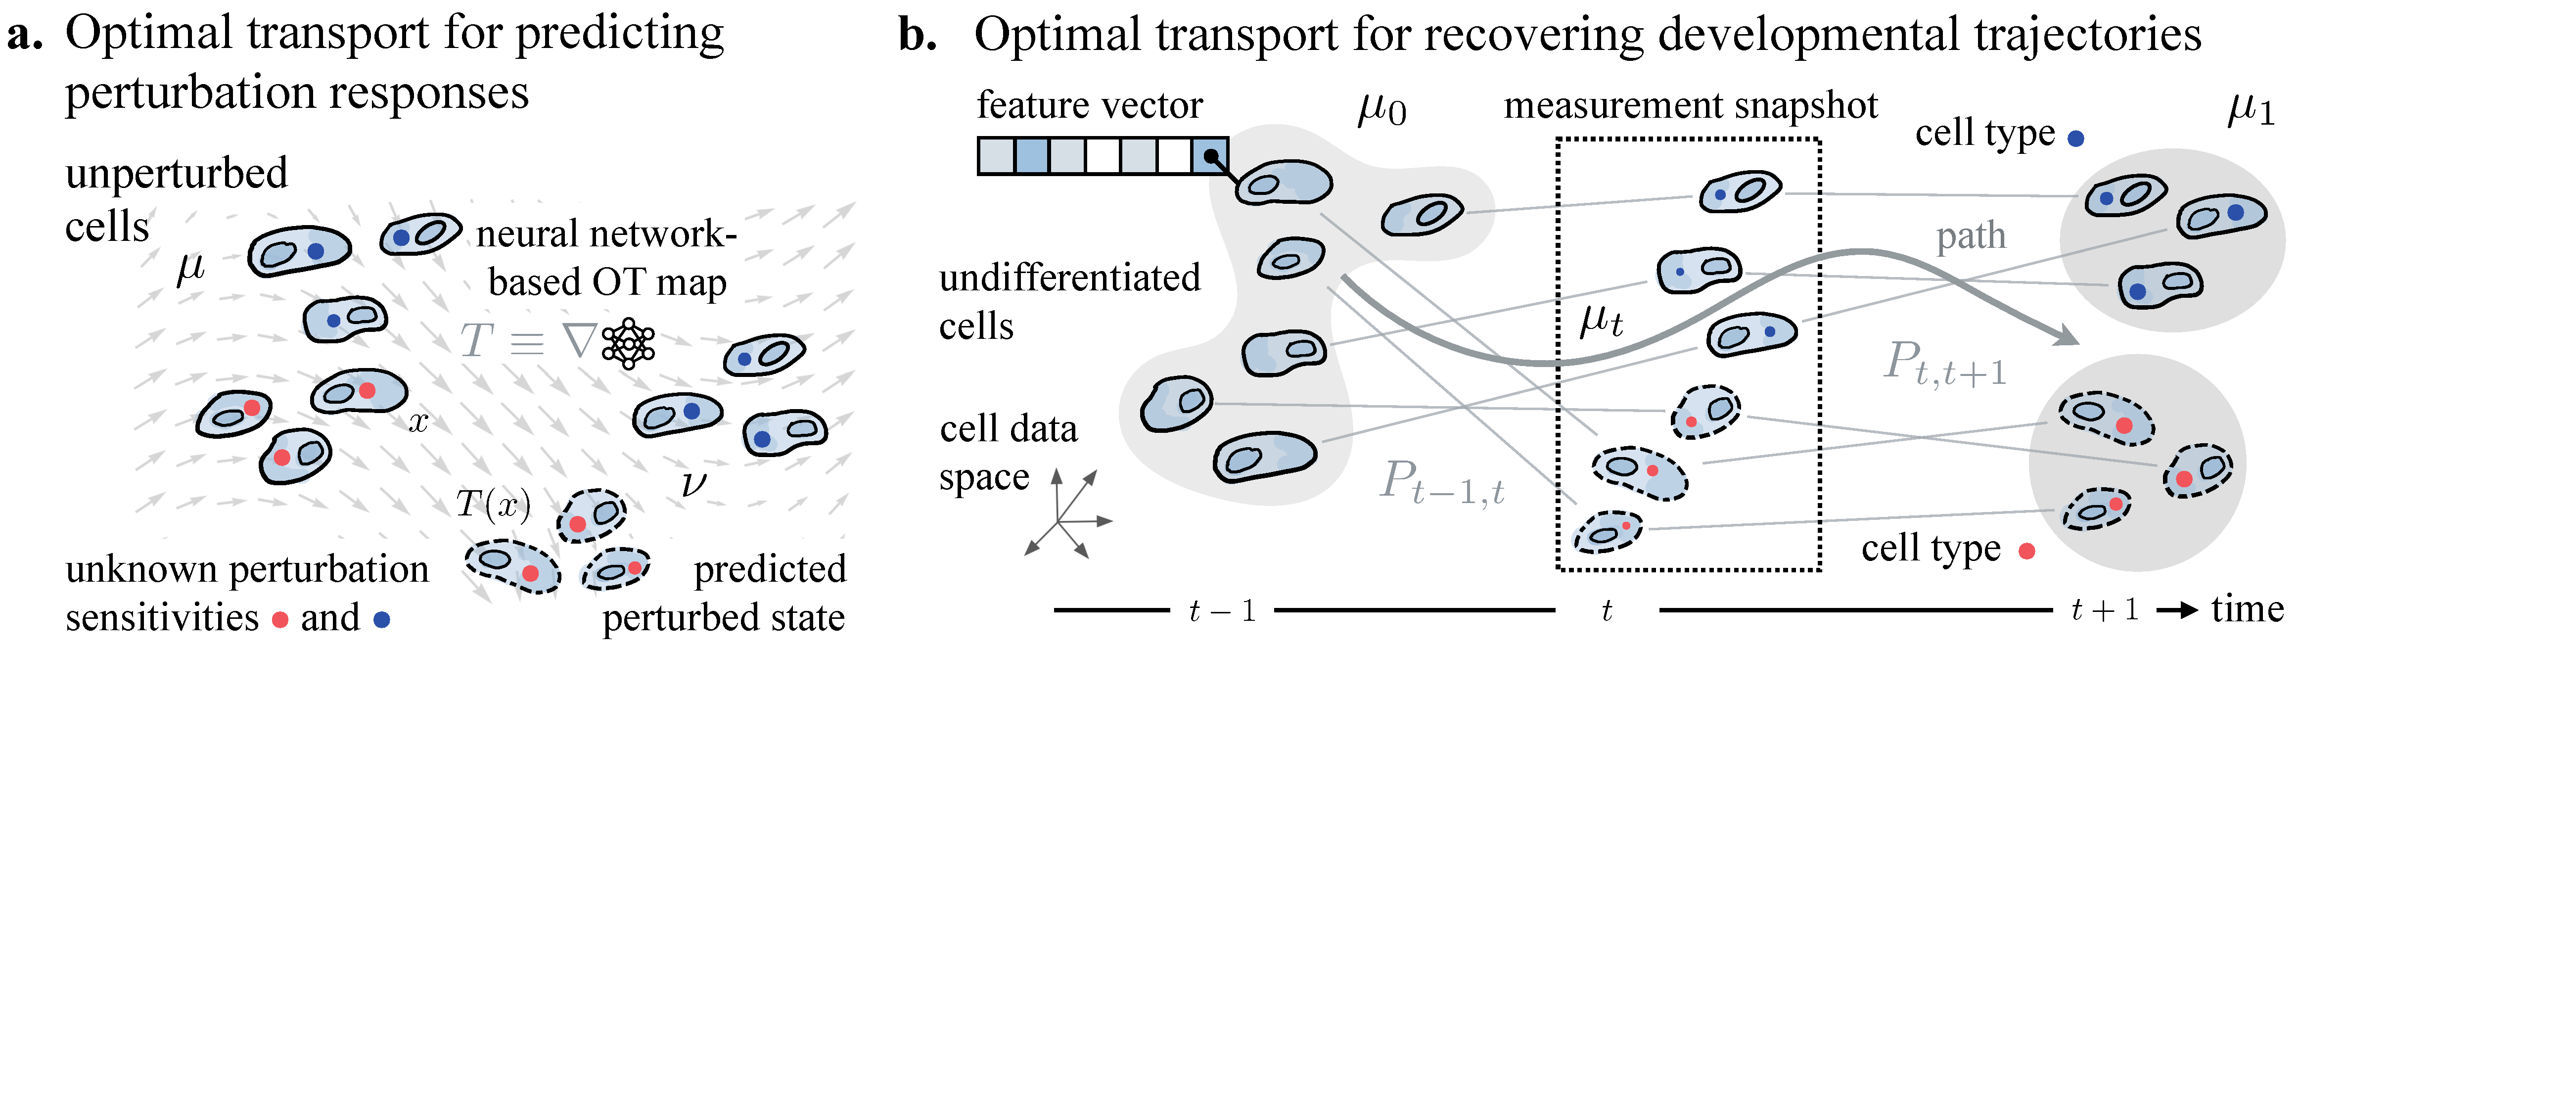
\includegraphics[width=\textwidth]{figures/fig_bio_problems.pdf}
  \caption{\textbf{Overview on different dynamical processes in biomedicine.} \textbf{a.} In order to understand and predict the response of an unperturbed cell population $\mu$ to a stimulus such as a therapeutic agent, we need to identify a map $T$ that explains its evolution into the perturbed population $\nu$. Then, the perturbed state of a cell $x$ is given by $T(x)$.  \textbf{b.} Developmental processes describe the evolution of a often homogeneous population of undifferentiated cells into various cell lineages. Reconstructing such processes from measurement snapshots can be achieved through sequential alignments $P_{t-1,t}$ that describe the evolution from $\mu_0$ to $\mu_1$, or by identifying the overall global path $\mu_t$ capturing the cell differentiation process.}
  \label{fig:bio_problems}
\end{figure}

\section{Cell Differentiation and Lineage Tracing in Developmental Biology}
\label{sec:cell_differentiation}

Complex cellular dynamics are not only initiated through external stimuli, but also at the core of developmental processes, tissue regeneration and formation.
The spectacular journey of a single zygote in the embryonic development, for example, metamorphosing into a complex, multicellular organism is largely governed by the mechanisms of cell differentiation, where pluripotent stem cells commit to specific lineages and mature into diverse cell types.

Understanding the molecular programs that guide such differentiation processes is a major challenge.
% Lineage tracing serves as a powerful tool to retrospectively track the genealogical origin of cells, helping to construct an in-depth chronicle of cellular development and differentiation. It unravels the developmental trajectory of cells, thereby facilitating the understanding of normal development as well as pathological conditions.
% However, capturing this process with accuracy poses profound challenges due to the stochastic nature of cell differentiation, technical complexities, and the vast temporal and spatial scales involved.
However, approaches relying on the bulk analysis of cell populations fall short in tackling these issues, as they fail to offer comprehensive solutions to two key obstacles: identifying various cell types within a population and tracking the development of each of these types.
By providing insights into the heterogeneity of cell populations, single-cell methods partially address the aforementioned challenges, but their destructive nature impedes the recording of the expression of the same cell and its direct descendants across time.
Hence, such differentiation processes can only be measured through distinct snapshots of single-cell populations that are \textit{not time-resolved} and \textit{unaligned}.

To understand differentiation ---the continuous emergence of different cell types and branching events--- we need to reconstruct such developmental processes from single-cell measurements that provide us with snapshots of the cell population evolving over time:
Given that a cell has a specific expression profile at a time point, where will its descendants likely be at a later time point and where are its likely ancestors at an earlier time point? 
\citet{schiebinger2019optimal} for example study reprogramming of fibroblasts to \acrfull{iPSC} \citep{takahashi2006induction}, by measuring \acrfull{MEF}. Cells at time point $t$ are connected to their ancestors at time $t-1$, by finding the corresponding transport plan $P_{t-1,t}$ between each pair of consecutive time steps (see \cref{fig:bio_problems}b).
To understand the overall dynamic process, however, this thesis aims at identifying the overall dynamic evolution of measure $\mu_t$ instead of resorting to the computation of distinct alignments between consecutive measurement snapshots \citep{lavenant2021towards}.


\section{Single-Cell High-Throughput Technologies}
\label{sec:tech_background}

Until recently, our understanding of cellular dynamics was limited to 'bulk' omics analyses, which yield average measurements for a cell population.
The advent of single-cell omics technologies has marked a significant shift from such average analyses, enabling a highly detailed examination of individual cells across various layers such as the genome, transcriptome, epigenome, and proteome.
This shift has revealed previously hidden complexities, such as rare cell types, transitional states, and cell-to-cell variability. Transformative techniques like single-cell RNA sequencing (\cref{sec:background_sequencing}) have allowed researchers to profile gene expression in thousands of cells simultaneously, shedding light on new cellular subpopulations and responses \citep{jia2022high}.
Additionally, modern imaging technologies have deepened our understanding of cell morphology and (the localization of) cellular signaling (\cref{sec:background_imaging}). 
The integration of these diverse omics layers provides a holistic view of cellular diversity, opening new avenues in the study of health, disease, and personalized medicine \citep{baysoy2023technological}.

Each point $x$ of such single-cell measurements then represents the recorded features of a single cell. Each feature (dimension) of that point tracks the expression level of each studied gene, or morphological and signaling feature strength in that cell, at measurement time. In this setting, a few thousand cells are sampled from a large population of cells, to obtain their features (high-throughput). This is done at distinct time points throughout cellular processes. Because of the destructive process of these measurements, each snapshot consists of several feature vectors, one for each different cell.
Two consecutive snapshots can be seen as two point clouds % that capture the heterogeneity of cells at each point in time. 
or, alternatively, as two tabular datasets $X = [x_1,\dots, x_n]$ and $Y=[y_1, \dots, y_m]$: Each of the $n$ or $m$ rows contains a cell and its $d$-dimensional feature representation, where each column denotes a particular feature, e.g., the activity of a gene.
In order to understand the temporal evolution of the cell population over time, we aim to provide an informed guess on an alignment or a map that relates the two cell populations $X$ and $Y$.
% In the following, we will discuss two different high-throughput technologies that allow us to record such features.

\subsection{Sequencing-Based Screening}
\label{sec:background_sequencing}

Sequence-based profiling methods have emerged as a transformative tool for understanding the complexity of biological systems at the resolution of individual cells. Methods such as single-cell \acrlong{RNA-seq} (scRNA-seq) or single-cell \acrlong{ATAC-seq} (scATAC-seq), enable us to characterize gene expression or chromatin accessibility within a single cell.
By mapping the transcriptomic or epigenomic landscapes of individual cells, sequence-based profiling methods have allowed for unprecedented insights into developmental biology, tissue homeostasis, disease pathology, and therapeutic responses.

RNA thereby serves a direct quantifier for gene activity: Genes in DNA are transcribed into \acrfull{mRNA}, which is then translated into proteins that carry out various functions within the cell.
By measuring the amounts and types of mRNA present in a cell at a given time, i.e., the transcriptome, we can understand which genes are being actively expressed. This information is valuable as changes in gene expression can signal various biological processes, such as cell development, responses to environmental stimuli, disease states, and much more. 
In order to record the gene expression in single cells, scRNA-seq requires isolating individual cells, often using techniques such as \acrfull{FACS} \citep{julius1972demonstration} or droplet-based technologies \citep{brouzes2009droplet, mazutis2013single, debs2012functional}. Each cell's mRNA is reverse transcribed into \acrfull{cDNA}, including a unique molecular identifier to correct for amplification bias.
This cDNA is then amplified and prepared for high-throughput sequencing and the resultant data provide insights into gene expression of individual cells.

Crucially, this process is destructive: Cells are destroyed, i.e., lysed, or broken open, in order to access the mRNA within and record their gene expression levels.
Once a cell is lysed, its structural integrity and function are lost, making it impossible to further manipulate or use that particular cell for subsequent experiments.
This is a fundamental limitation, as the process of obtaining the high-resolution molecular data comes at the expense of the cell's viability.

\subsection{Optical Phenotypic Screening}
\label{sec:background_imaging}

Optical phenotypic screening allows for the analysis of single cells based on their morphological and biochemical characteristics, with minimal perturbation to their natural state. 
Techniques such as fluorescence microscopy, time-lapse imaging, or flow cytometry typically involve labeling cells with fluorescent dyes or proteins that bind to or are expressed by specific cellular components of interest.
Such targets tagged with markers can be potential important components of signaling pathways or crucial regulators and indicators of core cellular functions. 
The cells are then imaged or passed through a laser, and the fluorescence emitted is captured and measured, providing information about the presence and quantity of the target molecules within each cell. 
The resulting images allow the extraction of morphological properties and the fluorescence intensity of each tag in different parts of each cell \citep{carpenter2006cellprofiler}.

However, it's important to note that while these methods are in general non-destructive in nature, some processes such as labeling or the use of certain dyes could potentially have some impact on cell viability or behavior. So while these techniques in general allow for dynamic tracking of cellular processes \citep{fischer2019inferring, hashimoto2016learning, tvarusko1999time, busch2015fundamental}, cells are usually fixed prior to staining to preserve cellular structures and allow for longer-term storage. Such procedures are lethal for cells, making longitudinal studies on the same cells impossible.

High-content imaging, particularly when augmented by multiplexing abilities, is ideally suited to study heterogeneous cell responses.
In this thesis, we study heterogeneous cell line responses to various cancer drugs based on a measurement technology known as \acrfull{4i} \citep{gut2018multiplexed}.
With 4i, fluorescently labeled antibodies are iteratively hybridized, imaged, and removed from a sample to measure the abundance and localization of proteins and their modifications. 
Thus, 4i quickly generates large, spatially resolved phenotypic datasets rich in molecular information from thousands of treated and untreated cells. Additionally to the multiplexed information generated by 4i, cellular and nuclear morphology are routinely extracted from microscopy images (without the need for 4i) by image analysis algorithms \citep{carpenter2006cellprofiler}.

% \section{Related Work on Studying Cell Dynamics}

% ...
% \citep{fischer2019inferring, busch2015fundamental, hashimoto2016learning, raue2015data2dynamics}

\section{Optimal Transport for Single-Cell Biology}
% TODO: Change labels if above section is written.
\label{sec:related_work_bio}
\label{sec:ot_for_biology}

Applied to the analysis and modeling of single-cell biology problems, OT has been used to infer the distributions of cells' ancestors and descendants along development \citep{schiebinger2019optimal}, perform trajectory inference \citep{bunne2022proximal, forrow2021lineageot, bunne2022recovering, lavenant2021towards, schiebinger2019optimal, tong2020trajectorynet, yang2020predicting, zhang2021optimal, chizat2022trajectory}, predict perturbation responses \citep{bunne2021learning, yang2018scalable, lubeck2022neural}, integrate multi-omics data of different modalities \citep{demetci2022scot}, infer cell-cell similarity \citep{huizing2022optimal}, and integrate across scales (e.g., morphology and molecular profiling) \citep{yang2021multi}. The increasing data complexity across multiple levels of biological organization, from molecular and cellular through spatial profiling \citep{moriel2021novosparc} of tissues, and imaging of organs, cement further the status of OT as an indispensable framework for high-throughput, multimodal, and multi-scale molecular, cell, tissue, and organ biology. The effectiveness of OT comes, however, with drawbacks: because the theory builds on extremely sophisticated mathematics that blends optimization \citep{cuturi2013sinkhorn, cuturi2022optimal}, stochasticity \citep{chizat2022trajectory, bunne2022recovering} and partial differential equations \citep{bunne2022proximal}, and, more recently, deep learning \citep{tong2020trajectorynet, bunne2021learning, bunne2022supervised, yang2018scalable, lubeck2022neural, yang2021multi}, its computations are challenging even by modern ML standards.


\cleardoublepage%
\chapter{Dynamical Processes in Biomedicine}
\label{cha:bio_background}

\dictum[Rosalind Franklin, \textit{Report} (1952)]{%
  The results suggest a helical structure (which must be very closely packed) containing probably 2, 3 or 4 coaxial nucleic acid chains per helical unit and having the phosphate groups near the outside.}%
\vskip 1em

...


\chapter{Optimal Transport for Dynamical Systems}
\label{cha:theory_background}

\dictum[Elinor Ostrom, \textit{Governing the Commons} (1990)]{%
  The power of a theory is exactly proportional to the diversity of situations it can explain.}%
\vskip 1em


Optimal transport theory~\citep{santambrogio2015optimal} is a core element of the machine learning toolbox and has become within a few years the go-to framework to analyze, model, and solve an ever-increasing variety of tasks involving probability measures. This is best exemplified by its increasing importance to fitting generative models, where the goal is to learn a map~\citep{arjovsky2017wasserstein, genevay2018learning, salimans2018improving}, or more generally a diffusion \citep{song2020score, de2021diffusion} to morph a simple measure (e.g., Gaussian) onto a data distribution of interest (e.g., images). This is also apparent in the many applications that use OT to align probability measures that have since arisen, e.g., to transfer label knowledge between datasets~\citep{flamary2016optimal, singh2020model}, to analyze sampling schemes~\citep{dalalyan2017theoretical}, or study population trajectories~\citep{schiebinger2019optimal, bunne2021learning}.

In this chapter, we primarily cast light on the static and dynamic formulation of optimal transport, and simultaneously establish their theoretical nexus by recalling its mathematical history from \citet{monge1781histoire} and \citet{kantorovich1942transfer} to modern Fields Medal winners \citet{villani2009optimal}, \citeauthor{figalli2010optimal}, and Abel Prize recipient \citet{caffarelli1990interior} in order to provide a solid foundation for the discussion ahead.


\section{Static Optimal Transport} \label{sec:background_ot_static}

\looseness -1 Optimal transport takes dual roles as it induces a mathematically well-characterized distance measure between distributions as well as provides a geometry-based approach to realize mappings between two probability distributions.
In this section, we introduce the mathematical foundations of the \textbf{static} OT problem. Further, we will provide an extended analysis of the \citeauthor{monge1781histoire} map, which provides an actionable way to flow from one probability distribution onto another.
We conclude with a complete proof of the celebrated \citeauthor{brenier1987decomposition} theorem. This quintessential result and its particularization to translation-invariant costs will lay the foundation of the flurry of neural approaches proposed in the literature. This includes modeling Monge maps as gradients of convex functions parameterized through convex neural networks \citep{amos2017input, huang2021convex, makkuva2020optimal, korotin2021neural, lubeck2022neural, bunne2022supervised}, i.e., approaches that are a direct consequence of the \citeauthor{brenier1987decomposition} theorem and subject of this thesis, regularizers \citep{uscidda2023monge}, amortized optimization \citep{amos2022amortizing, amos2022meta}, or entropic maps \citep{pooladian2021entropic, pooladian2023minimax, divol2022optimal, cuturi2023monge}.

\begin{figure}[t]
  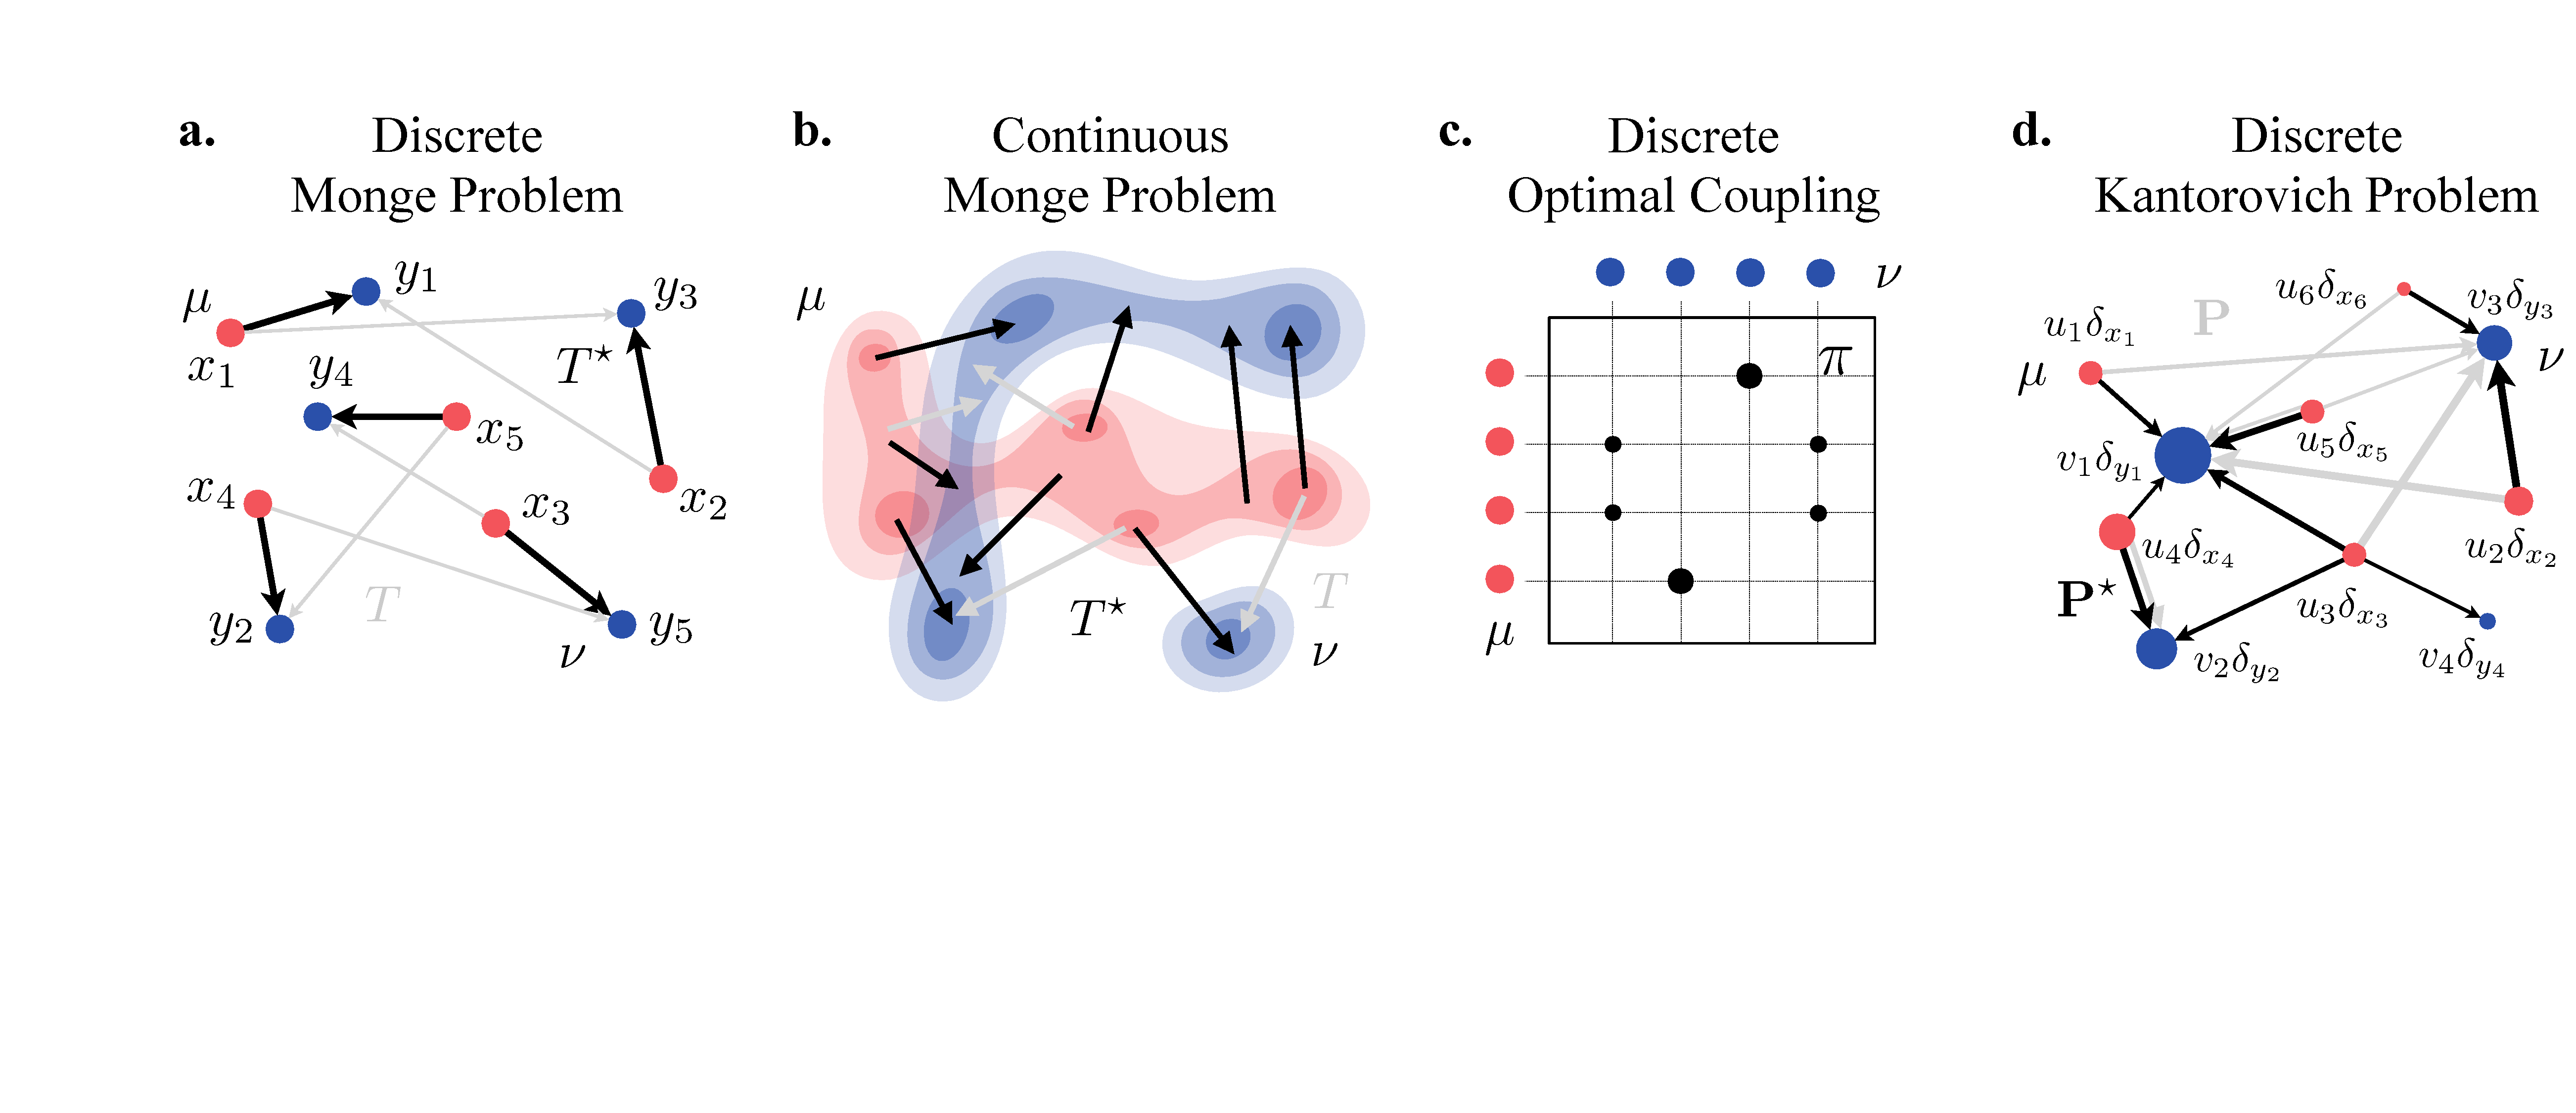
\includegraphics[width=\textwidth]{figures/fig_ot_background.pdf}
  \caption{\textbf{Overview on different formulations of the static OT problem for discrete and continuous measures.} Monge map for \textbf{a.} discrete and\textbf{b.} continuous measures $\mu, \nu$. The optimal map $T^\star$ minimizes \eqref{eq:monge}. \textbf{c.} Optimal coupling $\pi$ \eqref{eq:kantorovich} for discrete measures $\mu$ and $\nu$. \textbf{d.} Mass splitting principle of the Kantorovich relaxation for discrete measures $\mu$ and $\nu$ of the optimal transport plan $\bP^\star$ and a non-optimal plan $\bP$. Figure adapted from \citet{peyre2019computational}.}	
  \label{fig:ot_principles}
\end{figure}

\subsection{Monge Problem} \label{sec:background_monge}

In the 18th century "M{\'e}moire sur la th{\'e}orie des d{\'e}blais et des remblais", Gaspard Monge sets out to solve what is now known as the \citeauthor{monge1781histoire} problem, posing a seemingly simple, yet fundamentally complex question: Given two quantities of mass located at two different sites, what is the most efficient way into transport one to the other?
In more formal terms, provided with two measures $\mu, \nu\in \mathcal{P}(\mathbb{R}^d)$, here restricted to measures supported on $\mathbb{R}^d$, Monge's initial approach was to find a map $T$ that pushes one mass onto the other in a way that minimizes the total cost of transport.
Given a measurable const function $c: \mathcal{X} \times \mathcal{Y} \rightarrow \mathbb{R}$, the \citeauthor{monge1781histoire} problem then reads
\begin{equation}\label{eq:monge}
T^\star := \arg\inf_{T\sharp\mu=\nu}\int_{\mathbb{R}^d} c(x, T(x)) d\mu(x)\,.
\end{equation}
For two discrete measures $\mu=\sum_{i=1}^n u_i \delta_{x_{i}}, \nu=\sum_{j=1}^m v_j \delta_{y_{j}}$, it seeks a transport map $T: \mathcal{X} \rightarrow \mathcal{Y}$ associating each source point $x_i$ to a target point $x_j$ (see \cref{fig:ot_principles}a for the discrete and \cref{fig:ot_principles}b for the continuous setting).
...
The existence of $T^\star$ is guaranteed under fairly general conditions \citep[Theorem 1.22]{santambrogio2015optimal}, which require that $\mu$ and $\nu$ have finite $L_2$ norm, and that $\mu$ puts no mass on $(d-1)$ surfaces of class $\mathcal{C}_2$.


\subsection{Kantorovich Relaxation} \label{sec:background_kantorovich}

It was not until the 20th century, however, that the concept found a more tractable development. In \citeyear{kantorovich1942transfer}, Leonid \citeauthor{kantorovich1942transfer} provided a relaxation to this non-convex and difficult-to-solve problem.
Instead of the deterministic matching proposed by \citeauthor{monge1781histoire}, Kantorovich considered probabilistic correspondences that allow for transportation of mass from a single source point to various target points (mass splitting), resulting in
\begin{equation} \label{eq:kantorovich}
    W(\mu, \nu) = \inf_{\pi\in \Pi(\mu,\nu)}\iint c(x, y) \pi(dx, dy),
\end{equation}
where $\Pi(\mu, \nu) \defeq \left\{\pi \in \gP(\mathcal{X} \times \mathcal{Y}): P_{\gX \sharp} \pi=\mu \, \text { and } \, P_{\gY \sharp} \pi=\nu\right\}$ is the set of couplings on $\mathbb{R}^d\times\mathbb{R}^d$ with respective marginals $\mu, \nu$ (see \cref{fig:ot_principles}c).
For his work, \citeauthor{kantorovich1942transfer} received the Nobel Prize in economics. The connections of \acrshort{OT} to basic questions in economy becomes clear when interpreting $\mu$ as a density of resource units, and $\nu$ a density of factories, where the coupling $\pi$ denotes the optimal transportation plan of distributing resources to factories.

When instantiated on finite discrete measures, such as $\mu=\sum_{i=1}^n u_i\delta_{x_i}$ and $\nu=\sum_{j=1}^m v_j\delta_{y_j}$, this problem translates to a linear program, which can be regularized using an entropy term~\citep{cuturi2013sinkhorn,peyre2019computational}. For $\varepsilon\geq0$, set 
\begin{equation} \label{eq:reg-ot}
\We(\mu,\nu) \defeq \min_{\bP\in U(u, v)} \dotp{\bP}{[c(x_i, y_j)]_{ij}}  \,-\varepsilon H(\bP),
\end{equation}
where the discrete entropy is defined as $H(\bP) \defeq -\sum_{ij} \bP_{ij} (\log \bP_{ij} - 1)$ and the polytope $U(u, v)$ is the set of $n\times m$ matrices $\{\bP\in\mathbb{R}^{n \times m}_+, \bP\mathbf{1}_m =u, \bP^\top\mathbf{1}_n=v\}$. 
Notice that the definition above reduces to the usual Wasserstein distance when $\varepsilon=0$. Setting $\varepsilon>0$ yields a faster and differentiable proxy to approximate $W_{0}$, but introduces a bias, since $\We(\mu,\mu)\ne 0$ in general.
Thus, regularizing objective \eqref{eq:kantorovich} with an entropy term results in a significantly more efficient optimization \citep{cuturi2013sinkhorn} and differentiability w.r.t. its inputs. As a consequence, \eqref{eq:reg-ot} is commonly used as a loss function in machine learning applications, e.g., for structured prediction \citep{frogner2015learning,janati2020multi} or generative model fitting \citep{arjovsky2017wasserstein, salimans2018improving, genevay2018learning}.


\subsection{Kantorovich Duality} \label{sec:background_dual}

The Kantorovich formulation \eqref{eq:kantorovich} is a \emph{convex} problem on $\gP(\mathcal{X} \times \mathcal{Y})$ and thus admits a dual formulation by \citet{kantorovich1942transfer}, i.e., a constrained concave maximization problem defined as
\begin{equation} \label{eq:kantorovich-dual}
    W(\mu, \nu)=\sup _{(f, g) \in \Phi_{c}} \int f \mathrm{~d} \mu+\int g \mathrm{~d} v,
\end{equation}
\looseness -1 where the set of admissible potentials is $\Phi_c \defeq \{(f, g) \in L^{1}(\mu) \times L^{1}(\nu): f(x)+g(y) \leq c(x,y)$, $\forall(x, y) d\mu \otimes d\nu \text{ a.e.}\}$.
$(f, g)$ is thus a pair of continuous functions, often referred to as \emph{Kantorovich potentials}.
An informal interpretation of \eqref{eq:kantorovich-dual} was provided by \citet{caffarelli2003monge}, revisiting the connection of \acrshort{OT} to economics: 
A logistics company is concerned with transporting products from each resource unit $x$ to a factory $y$. The transportation company thereby charges $f(x)$ for loading resources at point $x$ and $g(y)$ of unloading it at destination $y$, but is constrained to charge $f(x)+g(y) \le c(x,y)$. In order to arrange prizes $f$ and $g$ that increase profit, they thus maximize objective \eqref{eq:kantorovich-dual}.

Beyond, using the notion of $c$-transforms, i.e.,
\begin{equation}
	\tag{$c$-transform}
	\forall y \in \mathcal{Y}, \quad f^c(y) \defeq \inf _{x \in \mathcal{X}} c(x, y)-f(x) \,,
\end{equation}
we can reduce \eqref{eq:kantorovich-dual} to a single potential: Assume we keep dual potential $f$ fixed, the potential $g$ needs to satisfy for all $x, y$
\begin{align*}
	f(x) + &g(y) \le c(x, y)\,,
	\forall y \in \mathcal{Y}, \quad  &g(t) \ge f^c(y) \defeq \inf _{x \in \mathcal{X}} c(x, y) - f(x)\,,
\end{align*}
resulting in the semi-dual
\begin{equation}\label{eq:semi-dual}
\arg\!\!\max_{f\, c\text{-concave}} \int f \textrm{d}\mu + \int f^c\textrm{d}\nu\,.
\end{equation}

\paragraph{Euclidean case.} For the cost $c(x, y) = \norm{x-y}^2$ in $\gX = \gY = \mathbb{R}^d$, one can replace the constraint of \eqref{eq:kantorovich-dual} using the Legendre-Fenchel transform
\begin{equation} \label{eq:legendre_fenchel}
	\tag{Legendre-Fenchel transform}
	\forall y, \quad g(y) \geq f^*(y) \defeq \sup _x\langle x, y\rangle-f(x)\,,
\end{equation}
where $f^*$ is the convex conjugate of $f$ and a convex function as a supremum of linear forms. Then, the semi-dual in the Euclidean setting reads
\begin{equation} \label{eq:dual-cvx}
	\arg\!\!\min_{f\, \text{convex}} \int f \textrm{d}\mu + \int f^*\textrm{d}\nu\,.
\end{equation}
Following further the double convexification trick as outlined in \citet[Lemma 2.10]{villani2021topics}, we see that applying the \ref{eq:legendre_fenchel} twice results in function pair $(f^{**},f^{*})$ and thus,  as each of them is defined as the supremum of a family of linear functions, an optimization problem over two convex lower semi-continuous functions.

\subsection{Brenier's Theorem} \label{sec:background_brenier}

Problem \eqref{eq:kantorovich-dual} allows us to characterize optimal transport plans that emerge as the solution to the Kantorovich optimal transportation problem \eqref{eq:kantorovich} and show sufficient conditions for the existence of optimal transport maps.
Although a large part of optimal transport theory can be developed in a general framework as above, for the rest of the section, we will resort to the case $c(x, y):=\|x-y\|^2$ on $\mathbb{R}^d \times \mathbb{R}^d$. Generalizations to other cost functions are possible but with an additional notational burden\footnote{For example it is possible to show the existence of optimal transport maps for strictly convex and superlinear cost functions, and characterize them in terms of $c$-superdifferentials of $c$-convex functions.}.
In the following, we will give a characterization of optimal transport plans \citep{knott1984optimal}:

\begin{theorem}[Knott-Smith Optimality Criterion]
	...
\end{theorem}
\begin{proof}
	For the complete proof, see \citet[Proof of Theorem 2.12]{villani2021topics}.
\end{proof}
In convex analysis this property is called cyclical monotonicity.

The next result specifically gives conditions sufficient for the existence of transport maps.
The celebrated \citeauthor{brenier1987decomposition} theorem \citeyearpar{brenier1987decomposition} establishes for the special case of the Euclidean distance the equivalence of the Monge \eqref{eq:monge} and Kantorovich formulation  \eqref{eq:kantorovich}, the uniqueness of the optimal coupling $\pi$, and states that there must exist a unique (up to the addition of a constant) potential $f^\star:\mathbb{R}^d\rightarrow \mathbb{R}$ such that $T^\star = \nabla f^\star$. 
This theorem has far-reaching implications: It is sufficient, when seeking optimal transport maps, to restrict the computational effort to seek a "good" convex potential, such that its gradient pushes $\mu$ towards $\nu$. 
More formally:

\begin{theorem}[Brenier's Theorem] \label{thm:brenier}
	In the setting where both $\mathcal{X}$ and $\mathcal{Y}$ are equal to $\mathbb{R}^d$, and the cost function $c(x, y) = |x-y|^2$ is employed, and at least one of the two input measures $\mu$ possesses a density $\rho_\mu$ in relation to the Lebesgue measure, then there exists a unique optimal solution $\pi$ in the Kantorovich formulation \eqref{eq:kantorovich}.
	This solution is exclusively supported on the graph $(x, T(x))$ of Monge map $T: \mathbb{R}^d \rightarrow \mathbb{R}^d$.
	In other terms, we can express $\pi$ as $(\operatorname{Id}, T)_{\sharp} \alpha$, meaning that for any function $h$ belonging to the set $\forall h \in \mathcal{C}(\mathcal{X} \times \mathcal{Y})$, the following equality holds
	$$
	\quad \int_{\mathcal{X} \times \mathcal{Y}} h(x, y) \mathrm{d} \pi(x, y)=\int_{\mathcal{X}} h(x, T(x)) \mathrm{d} \mu(x).
	$$
Moreover, this map $T$ is uniquely determined by the gradient of a convex function $\varphi$, denoted as $T(x)=\nabla \varphi(x)$. The function $\varphi$ is the unique convex function, up to an additional constant, for which $(\nabla \varphi)_{\sharp} \mu=\nu$. We can establish a relationship between this convex function $\varphi$ and the dual potential $f$ that solves \eqref{eq:kantorovich-dual} by expressing $\varphi(x)$ as $\frac{|x|^2}{2}-f(x)$.
\end{theorem}
\begin{proof}
	...
\end{proof}
...
\begin{corollary}
	Under the assumption of \cref{thm:brenier}, $\nabla \varphi$ is the unique solution to the Monge transportation problem \eqref{eq:monge}, i.e.,
	\begin{equation}
		\int_{\mathbb{R}^d} \norm{x-\nabla \varphi(x)}^2 \mathrm{d}\mu(x) = \inf_{T_\sharp \mu = \nu} \int_{\mathbb{R}^d}\norm{x - T(x)}^2 \mathrm{d}\mu(x).
	\end{equation}
\end{corollary}
This result has been exploited to propose neural OT solvers ~\citep{makkuva2020optimal, korotin2021wasserstein, bunne2022proximal, alvarez2021optimizing, mokrov2021large} and  will recurrently permeate this thesis, proving its essential nature in multiple instances and modern developments of optimal transport.
In particular, it presents an elegant way to solve the Monge problem in a geometric sense and has profound implications for the dynamic version of the problem, which we will study next.


\section{Dynamic Optimal Transport} \label{sec:background_ot_dynamic}

We have hitherto engaged with the \emph{static} \acrlong{OT} problem, establishing a solid foundation upon which to build more intricate dynamic formulations. In fact, the roots of these dynamic formulations are embedded within the static \acrshort{OT} framework: As posited by \citet{benamou2000computational}, the dynamic formulation "was already implicitly contained in the original problem addressed by Monge" \citep{monge1781histoire}, where "eliminating the time variable was just a clever way of reducing the dimension of the problem." When reintroducing time in the dynamic version, the optimal transport map becomes a time-dependent flow capable of describing the evolution of a measure over time.

In this section, we will cover several perspectives and frameworks of the \textbf{dynamic} \acrshort{OT} problem: Brenier's theorem thereby forms a critical bridge that connects the static and dynamic formulation, perpetuated in the Monge-Amp{\`e}re equation.
Further, \citet*{benamou2000computational} introduce how the dynamic point of view offers an alternate and intuitive interpretation of optimal transport with links to fluid dynamics. The resulting framework surprisingly leads to a convex optimization problem that can be parameterized through normalizing flows \citep{tong2020trajectorynet}.
We further highlight the connections of \acrshort{OT} to \acrshortpl{PDE} such as Fokker-Planck-like equations through the \citeauthor*{jordan1998variational} scheme.
Lastly, moving beyond PDEs and taking a stochastic control perspective, we will introduce the notion of the Schr\"odinger bridge problem


\subsection{Monge-Amp{\`e}re Equation} \label{sec:background_monge_ampere}

% Caffarelli's regularity theorems from the 1990s represented a major breakthrough in our understanding of the Monge-Amp{\`e}re equation, a highly nonlinear, quintessential partial differential equation, that for instance is used to construct surfaces of prescribed Gaussian curvature. Important existence results were established by Alexandrov, and earlier central properties had been shown by Caffarelli in collaboration with Nirenberg and Spruck, with further key contributions by Evans and Krylov. Caffarelli however closed the gap in our understanding of singularities by proving that the explicitly known examples of singular solutions are the only ones.

% Caffarelli has, together with collaborators, applied these results to the Monge-Kantorovich optimal mass transportation problem, based on previous work by Brenier. Caffarelli and Vasseur gave deep regularity results for the quasi-geostrophic equation in part by applying the exceptionally influential paper by Caffarelli and Silvestre on the fractional Laplacian.
As a direct consequence of \cref{thm:brenier}, if $T(x) = \nabla \varphi(x)$, $\varphi$ are smooth and strictly convex, and $\mu$ and $\nu$ absolutely continuous with densities $\rho_\mu$ and $\rho_\nu$, then we can express $T_\sharp \mu = \nu$ in a nonlinear \acrfull{PDE} form. More concretely, $\varphi$ is a solution of the Monge-Amp{\`e}re equation that reads
\begin{equation} \label{eq:monge_ampere}
	\operatorname{det}\left(\partial^2 \varphi(x)\right) \rho_\nu(\nabla \varphi(x))=\rho_\mu(x),
\end{equation}
where $\partial^2 \varphi(x) \in \mathbb{R}^{d \times d}$ is the Hessian of $\varphi$, describing the continuous evolution from $\mu$ to $\nu$.
The regularity of the solutions of \eqref{eq:monge_ampere}, with implications on regularity results of the optimal transport map $T$, has been subject of a series of works by \citeauthor{caffarelli1990interior} in the \citeyear{caffarelli1990interior}s, for which he was awarded the Abel Prize in 2023, as well as more recently by \citeauthor{figalli2017monge}, recognized with the Fields Medal in 2023.
...

\subsection{Benamou-Brenier Formulation} \label{sec:background_benamou_brenier}

Avoiding solving \eqref{eq:monge_ampere} directly, \citet{benamou2000computational} introduce an alternative numerical framework by connecting the optimal mass transfer problem to continuum mechanics frameworks.
Deviating from the previous notation of $(\mu, \nu)$, in the following sections we study the dynamic problem via the evolution from measure $\mu_0$ at time $t=0$ to $\mu_1$ at $t=1$. The solution of \eqref{eq:kantorovich} then coincides with finding the minimal path $(\mu_t)_{t=0}^1$, or more concretely, a curve in the space of measures minimizing a total length.  
Such path $\mu_t$ can be described by a vector field $v_t$ satisfying the continuity equation in fluid dynamics or conservation of mass formula
\begin{equation} \label{eq:continuity_equation}
	\frac{\partial \mu_t}{\partial t}+\nabla\left(\mu_t v_t\right)= 0, \qquad \mu_{t=0}=\mu_0, \mu_{t=1}=\mu_1\,,
\end{equation}
where the vector field $v_t$ denotes the speed and $J_t = \mu_t v_t$ corresponds to the momentum. 
Every curve $\mu_t$ describing the evolution of the measure over time can thereby be interpreted as the fluid flow along a family of vector fields. We are searching for the vector field $v_t$ that (i.) that satisfies the conservation of mass \eqref{eq:continuity_equation}, and (ii.) minimized the path length.
The infinitesimal length of such a vector field can be computed via 
\begin{equation*}
	\left\|v_t\right\|_{\ell^2\left(\mu_t\right)}=\left(\int_{\mathbb{R}^d}\left\|v_t(x)\right\|^2 \mathrm{~d} \mu_t(x)\right)^{1 / 2},
\end{equation*}
resulting, in the case of $\gX = \gY = \mathbb{R}^d$ and $c(x, y)=\|x-y\|^2$, in the minimal-path reformulation of \eqref{eq:kantorovich}
\begin{equation} \label{eq:benamou_brenier}
	\min _{\left(\mu_t, v_t\right) t \text { sat. \eqref{eq:continuity_equation}}} \int_0^1 \int_{\mathbb{R}^d}\left\|v_t(x)\right\|^2 \mathrm{~d} \mu_t(x) \mathrm{d} t\,.
\end{equation}
To further provide a physical interpretation, selecting a vector field $v_t$ that minimizes $\int_{\mathbb{R}^d}\left\|v_t(x)\right\|^2$ can thereby be seen as minimizing a kinetic energy.
Reciting \cref{thm:brenier}, with $T = \nabla \varphi$, $\mu_t$ is equal to \citeauthor{mccann1997convexity}'s interpolation between $\mu_0$ and $\mu_1$
\begin{equation} \label{eq:mccann_interpolation}
	\mu_t = [(1-t) I+t \nabla \varphi]_\sharp \mu_0 = [(1-t) I+t \nabla T]_\sharp \mu_0\,.
\end{equation}


\subsection{Jordan-Kinderlehrer-Otto Flows} \label{sec:background_jko}

$\{ \mu_t ; 0 \leq  t \leq  1\}$ may be seen as a constant-speed geodesic interpolating between population $\mu_0$ and $\mu_1$ in the space of measures \citep{otto2001geometry}.
The analysis of such curves, Wasserstein geodesics often referred to as displacement or \citeauthor{mccann1997convexity} interpolation, has led to a variety of applications:
In particular, following \citet{otto2001geometry} on the calculus of optimal transport (\citeauthor{otto2001geometry} calculus), a large class of PDEs may be viewed as gradient flows on the Wasserstein space \citet{jordan1998variational}.
A gradient flow is a curve following the direction of steepest descent of a function $F$.
Considering the evolution of a vector $x$ over time in the Euclidean space, with $F$ being smooth, this can be realized through the standard gradient descent (forward) scheme
\begin{equation*}
	x_{t+1} \defeq x_{t}-\tau \nabla F\left(x_{t}\right)\,,
\end{equation*}
where $\tau$ is the step size. For non-smooth functions, on can resort to a proximal (backward) scheme, i.e.,
\begin{equation*}
	x_{t+1} \defeq \operatorname{Prox}_{\tau F}^{\|\cdot\|}\left(x_{t}\right) \defeq \arg\!\min_x \frac{1}{2}\left\| x-x_t\right\|^2+\tau F(x)\,.
\end{equation*}
When studying the evolution of measure $\mu_t$ over time, we will resort to optimal transport metrics the $\ell_2$-norm $\norm{\cdot}$.
Considering a functionals $F$ taking a measure as input, a gradient flow of $\mu$ w.r.t. to $F$ 
\begin{equation}
	\mu_{t+1} \defeq \arg\!\min_\nu W(\mu, \mu_t)^2+\tau F(\mu)\,.
\end{equation}


In recent works \citep{bunne2022proximal, alvarez2021optimizing, mokrov2021large, benamou2016augmented} \acrshort{JKO} flows have found application in inferring the evolution of populations over time, crucial in many scientific disciplines when for instance, observing a population of cells in biology.

\subsection{Stochastic Control Perspective} \label{sec:background_control}

...

\subsection{Schr{\"o}dinger Bridges} \label{sec:background_sb}

...
In his work "{\"U}ber die Umkehrung der Naturgesetze" published in \citeyear{schrodinger1931umkehrung}, Erwin Schr{\"o}dinger studied the most likely random evolution between two given marginals for a cloud of diffusive particles.

It's connections to optimal transport might not be clear at first. ...

It represents a key connection that has recently fueled the development of \acrlongpl{DSB} \citep{de2021diffusion, chen2021stochastic, bunne2022recovering, liu2022deep}. Compared to classical diffusion-based generative models \citep{daniels2021score, song2020score}, these algorithms allow interpolation between complex distributions. Extended to the Riemannian geometry \citep{thornton2022riemannian, de2022riemannian}, it has found applications in molecular dynamics \citep{holdijk2022path, somnath2023aligned} and cell differentiation processes \citep{vargas2021solving, bunne2022recovering, tong2023conditional}.



\part{Static Neural Optimal Transport} \label{part:static_not}
\cleardoublepage%
\chapter{Neural Optimal Transport}
\label{cha:cellot}


\dictum[Gottfried Wilhelm Leibniz, \textit{Nouveaux essais sur l'entendement humain} (1765)]{%
  Tout va par degr\'e dans la nature, et rien par saut, et cette regle \`a l'\'egard des changements est une partie de ma loi de la continuit\'e.}%
\vskip 1em

\verpar{Contributions}{
Most of the material in this chapter has been already published in the following journal article:
\begin{itemize}
	\item[] Charlotte Bunne, Stefan G Stark, Gabriele Gut, Jacobo Sarabia del Castillo, Kjong-Van Lehmann, Lucas Pelkmans, Andreas Krause, and Gunnar R{\"a}tsch. Learning Single-Cell Perturbation Responses using Neural Optimal Transport. \textit{Nature Methods}, 2023.
	\vspace{-9pt}
\end{itemize}
}

\begin{figure}
    \centering
    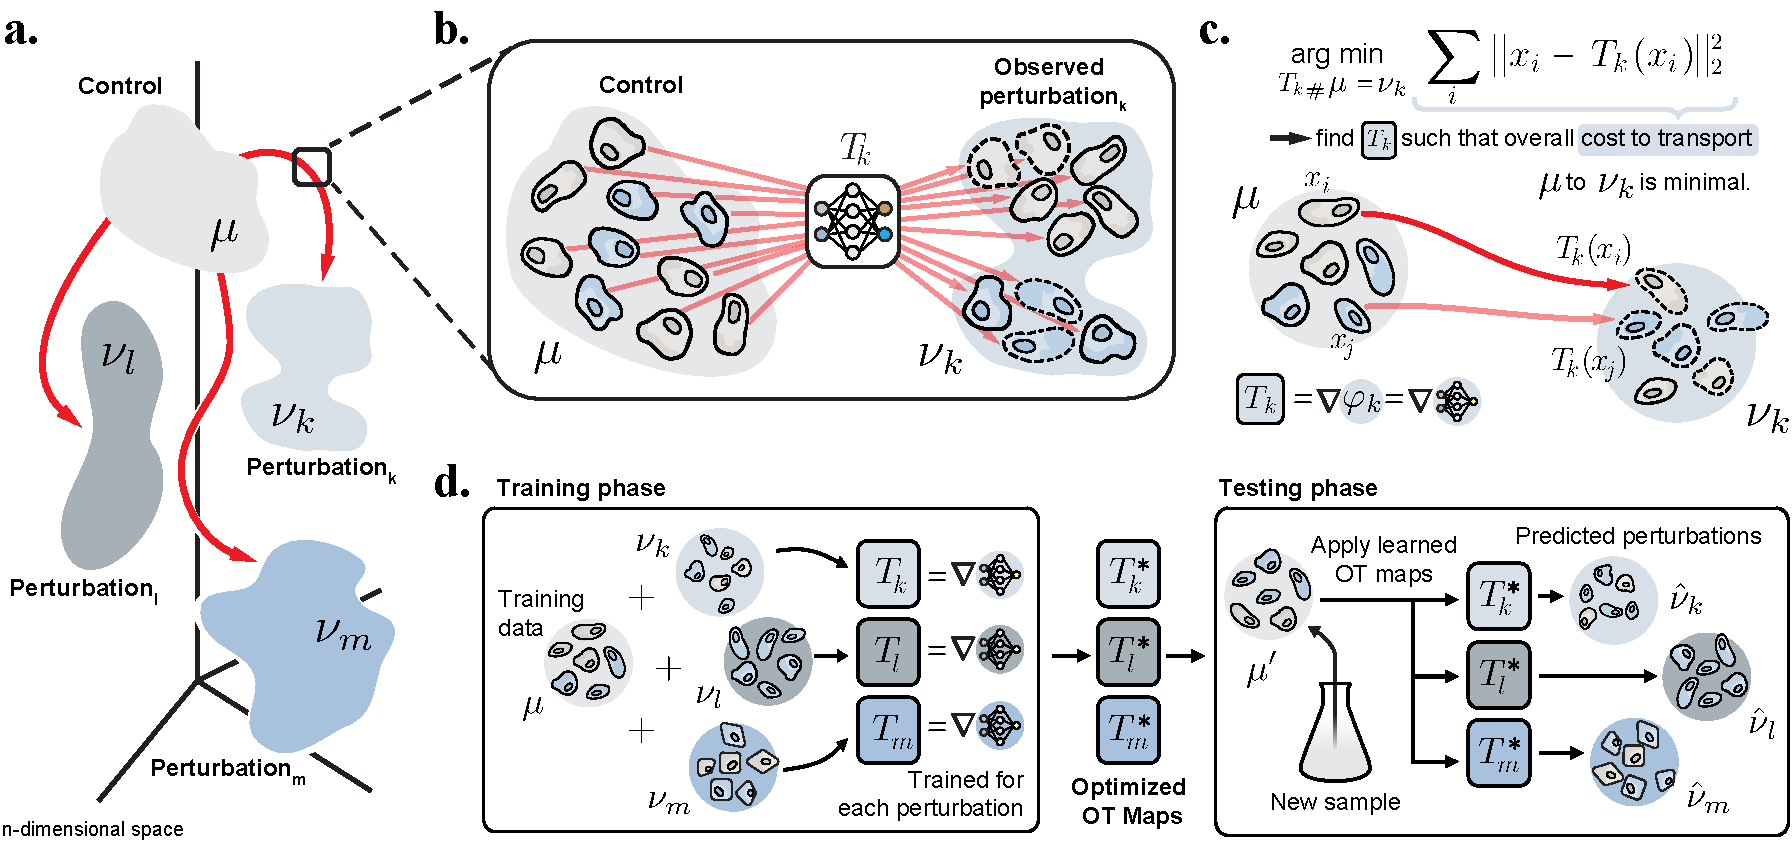
\includegraphics[width=\textwidth]{figures/fig_overview_cellot.pdf}
    \caption{\textbf{Overview of the \textsc{CellOT} Model.} \textbf{a.}~Distributions of single cells were measured in either an untreated control state ($\mu$) or in one of several perturbed states ($\nu_k, \nu_l, \nu_m,  \ldots$). These distributions lie in a high-dimensional space of profiled features. \textbf{b.}~For a perturbation $k$, we aim to model it with a function $T_k$ that maps untreated cells in $\mu$ to their treated counterparts in $\nu_k$. \textbf{c.}~Lacking paired measurements, we assume that the perturbation transforms $\mu$ into $\nu_k$ under a principle of minimal effort. In particular, we learn $T_k$ using optimal transport theory to directly estimate this distributional mapping as the gradient of the optimal transport dual potential $\nabla g_\theta$.
    \textbf{d.}~OT maps are learned for all perturbations independently. Because these maps are fully parameterized, \textsc{CellOT} can be trained, for example, on a set of initially provided samples to then make predictions on untreated cells originating from new, previously unseen samples.}
    \label{fig:overview_cellot}
\end{figure}


Characterizing and modeling perturbation responses at the single-cell level from non-time-resolved data remains one of biology's grand challenges. It finds applications in predicting cellular reactions to environmental stress or a patient's response to drug treatments. Accurate inference of perturbation responses at the single cell level allows us, for instance, to understand how and why individual tumor cells evade cancer therapies \citep{frangieh2021multimodal}. More generally, it deepens the mechanistic understanding of the molecular machinery that determines the respective responses to perturbations. Single-cell responses to genetic or chemical perturbations are  highly heterogeneous~\citep{liberali2014hierarchical} due to multiple factors, including pre-existing variability in the abundance and subcellular organization of mRNA and proteins~\citep{battich2013image, battich2015control, gut2018multiplexed, shaffer2017rare}, cellular states~\citep{kramer2019cellular}, and the cellular microenvironment~\citep{snijder2009population}. To effectively predict the drug response of each cell in a  population, whether derived from tissue culture or as primary cells from a patient biopsy, it is thus crucial to incorporate this heterogeneous multivariate subpopulation structure into the analysis.

\looseness -1 A fundamental difficulty in learning perturbation responses is that cells are usually fixed and stained or chemically destroyed to obtain these measurements. Hence, it is only possible to measure the same cells  before or after a perturbation is applied. 
Therefore, while we do not have access to a set of {\em paired} control/perturbed single-cell observations, we do have access to separate \emph{sets} of single-cell observations from control and perturbed cells, respectively. To subsequently match single cells between conditions and, at the same time, account for cellular heterogeneity is a highly complex pairing problem.

Here, we seek to learn a perturbation model that robustly describes the cellular dynamics upon intervention while still accounting for underlying variability across samples. Learning the responses on an existing patient cohort enables inference of treatment responses for new, i.e., previously unseen patients, assuming that we captured the heterogeneous drug reactions of patients during training.
It is crucial, however, to not simply model average perturbation responses of a patient cohort, but to capture the specificities of a single patient through personalized treatment effect predictions.
% Even though we seek a robust and coherent model, we must ensure that we propose personalized treatment effect predictions rather than average perturbation responses of a patient cohort possibly not capturing the specificities of a single patient.

\looseness -1 Previous methods to approximate single-cell perturbation responses fall short of solving this highly complex \emph{pairing} problem while, at the same time, accounting for cellular heterogeneity and the strong subpopulation structure of cell samples~\citep{wu2021single,gonzalez2020tumor,li2022single}. 
Current state-of-the-art methods~\citep{lopez2018scvi, lotfollahi2019scgen, yang2020predicting} predict perturbation responses via \emph{linear shifts} in a learned % low-dimensional
latent space.
While this can capture nonlinear cell-type-specific responses, the use of linear interpolations reduces the alignment problem to the possibly more challenging task of learning representations that are invariant to the corresponding perturbation. \\

\looseness -1 In this chapter, we introduce \textsc{CellOT}, a novel approach that predicts perturbation responses of single cells by \emph{directly} learning and uncovering maps between control and perturbed cell states, thus explicitly accounting for heterogeneous subpopulation structures in multiplexed molecular readouts.
Assuming perturbations incrementally alter molecular profiles of cells, such as gene expression or signaling activities, we learn these changes and alignments using a static \acrlong{OT} formulations (see \cref{sec:background_ot_static}). 
As described in \cref{sec:ot_for_biology}, it has found recent successes modeling cellular developmental processes~\citep{lavenant2021towards, schiebinger2019optimal}, albeit in a {\em non-parameterized} setting. Thus, such OT-based approaches are unable to make predictions on unseen cells, such as those from unseen samples, e.g., new patients. 
% One way to address the pairing problem is to assume that perturbed cellular states are coupled to their initial states under a principle of minimum action. That is, given unpaired observations of cells before and after perturbation, we would aim to pair cells to their treated states in such a way that the average distance between the pairs, in feature space, is minimal. This setting is ideally suited for acute cellular perturbations during which single cells do not redistribute entirely and randomly in multidimensional measurement space, but typically only in a few dimensions, maintaining the overall correlation structure.

\looseness -1 In the following, we propose a neural optimal transport-based approach for inferring single-cell perturbation responses. 
Our method, \textsc{CellOT}, learns an optimal transport map for each perturbation in a fully parameterized and highly scalable manner. Instead of directly learning a transport map~\citep{korotin2021wasserstein, yang2018scalable, prasad2020optimal}, \textsc{CellOT} parameterizes a pair of dual potentials \eqref{eq:dual-cvx} with convex neural networks \citep{amos2017input}. This choice induces an important theory-motivated inductive bias essential to model stability~\citep{makkuva2020optimal}. 

\looseness -1 We demonstrate \textsc{CellOT}'s effectiveness by (i.) learning single-cell marker responses to different cancer drugs in melanoma cell lines, (ii.) predicting single-cell transcriptome responses in biopsies of patients with systemic lupus erythematosus as well as Panobinostat treatment outcomes of glioblastoma patients, (iii.) inferring \acrfull{LPS} responses across different animal species, and (iv.) modeling the transcriptome evolution of cell fates in hematopoiesis. Moreover, we benchmark \textsc{CellOT} against current state-of-the-art methods on multiple tasks~\citep{lopez2018scvi, lotfollahi2019scgen, chen2020dissecting}.

\section{Neural Optimal Transport Solvers} \label{sec:neural_solvers}

To generalize optimal transport formulations to the out-of-sample setting, recent efforts have concentrated on developing parameterizations of neural optimal transport schemes.
While initial efforts concentrated on solving large-scale \acrshort{OT} problems \citep{seguy2018large}, the focus quickly moved to \acrfull{GAN} \citep{arjovsky2017wasserstein, genevay2018learning}.
The majority of existing methods thereby employ \acrshort{OT} as a loss function to compute the discrepancy between the model and the data (target) distribution. 
More recently, however, the focus has shifted to parameterizing the \acrshort{OT} map $T$ \eqref{eq:monge} \citep{yang2018scalable, rout2021generative, daniels2021score}. Such parameterized OT maps not only function as generative models but extend to tasks that involve interpolations between distributions. More concretely, neural network-based parameterizations of $T$ allow us to model the evolution from a measure $\mu$ into a measure $\nu$ \citep{tong2020trajectorynet}, i.e., the focus of this thesis.

Multiple strategies exist on how to parameterize the optimal transport problem.
In the following, we consider neural \acrshort{OT} solvers that make direct use of the \citeauthor{brenier1987decomposition} theorem (\cref{thm:brenier}) and are based on the semi-dual \eqref{eq:dual-cvx}. For a review of alternative approaches, see \cref{sec:other_neural_solvers}.
For convenience, let us restate the semi-dual formulation in \eqref{eq:dual-cvx}
\begin{equation*}
	\varphi^\star \leftarrow \arg\inf_{\varphi\, \text{convex}} \int \varphi \textrm{d}\mu + \int \varphi^*\textrm{d}\nu\,,
\end{equation*}
where the optimization problem is concerned with finding a convex function $\varphi$ and its convex conjugate \eqref{eq:legendre} $\varphi^*$ given by
\begin{equation} \label{eq:varphi_conjugate}
	\forall y, \quad \varphi^*(y) \defeq \sup _x \langle x, y\rangle-\varphi(y)\,.	
\end{equation}
As discussed in \cref{sec:background_brenier}, the optimal transport map $T^\star$ for cost $c(x,y) = \|x-y\|^2_2$ and $\gX = \gY = \mathbb{R}^d$ in~\eqref{eq:monge} can be recovered via $\nabla \varphi^\star$.

As the convex conjugate $\varphi^*$ is very hard to compute, \citet{makkuva2020optimal} propose to approximate it via another convex function $g$.
Thus, to learn the optimal transport map, the approach builds upon celebrated results by \citet{knott1984optimal} and \citet{brenier1991polar}, which relate the optimal solutions for the primal \eqref{eq:monge} and the dual form \eqref{eq:kantorovich-dual}, to derive a min-max formulation that approximates Monge map $T$ \citep[Theorem 3.3]{makkuva2020optimal}.
The resulting objective reads
\begin{equation} \label{eq:ot-minmax}
	\arg \max_{\varphi  \, \text{convex}} \min_{g \, \text{convex}}  -\int \varphi(x) \mathrm{d} \mu(x) -\int \langle y, \nabla g(y)\rangle - \varphi(\nabla g(y)) \,\mathrm{d} \nu(y)\,.
\end{equation}
The intuition behind the approach stems from the fact that
\begin{equation*}
	\int \varphi^*\textrm{d}\nu = \sup _{g \text{ convex}} \int \langle y, \nabla g(y)\rangle - \varphi(\nabla g(y))\,\mathrm{d} \nu(y)\,.
\end{equation*}
We observe that in $\langle y, \nabla g(y)\rangle - \varphi(\nabla g(y)) \leq \varphi^*(y)$ for all functions $g$ the equality is achieved with $g = \varphi^*$ \citep[Theorem 3.3]{makkuva2020optimal}. 

In order to solve the optimization problem stated in \eqref{eq:ot-minmax}, \citet{makkuva2020optimal} parameterize both potentials $\varphi$ and $g$ using \acrfull{ICNN} (\cref{sec:icnns}), i.e., neural networks that parameterize the class of convex functions \citep{amos2017input}, such that
\begin{align} \label{eq:cellot-optim}
	\nonumber \theta^\star, \phi^\star \leftarrow \arg \max_{\varphi_\theta  \, \text{convex}} \min_{g_\phi \, \text{convex}}  &-\int \varphi_\theta(x) \mathrm{d} \mu(x) -\int \langle y, \nabla g_\phi(y)\rangle \\
	&- \varphi_\theta(\nabla g_\phi(y)) \,\mathrm{d} \nu(y),
\end{align}
where $\theta$ and $\phi$ are the parameters of each \acrshort{ICNN}.
Thus, the potentials $\varphi$ and $g$ can be learned via an alternate min-max optimization problem with loss functions
% TODO: Double-check.
\begin{align} 
	\label{eq:makkuva_f_loss}
    \ell_\varphi(\mu, \nu; \theta) &= \mathbb{E}_{x \sim \mu}[\text{ICNN}_{\phi}(x)] - \mathbb{E}_{y \sim \nu}[\text{ICNN}_{\theta}(\nabla \text{ICNN}_{\phi}(y))],   \\
    \label{eq:makkuva_g_loss}
    \ell_g(\mu, \nu; \phi) &= -\mathbb{E}_{y \sim \nu}[\langle y, \nabla \text{ICNN}_{\phi}(y)\rangle-\text{ICNN}_{\theta}(\nabla \text{ICNN}_{\phi}(y))].
\end{align}
For more details, see \citet{makkuva2020optimal, korotin2021neural}.


\subsection{Convex Neural Architectures}
\label{sec:icnns}

Input convex neural networks are neural networks $\varphi_\theta(x)$ with specific constraints on the architecture and parameters $\theta$, such that their output is a convex function of some (or all) elements of the input $x$~\citep{amos2017input}. We consider  \acrshortpl{ICNN}, such that the output is a convex function of the entire input $x$. A typical \acrshort{ICNN} is a $L$-layer, fully connected network such that, for $l = 0, \dots, L-1$:
\begin{equation} \label{eq:icnn}
    z_{l+1} = a_l(W^x_lx + W^z_l z_l + b_l)  \text{ and } \varphi_\theta(x) = z_L,
\end{equation}
where by convention, $z_0$ and $W^z_0$ are $0$, $a_l$ are convex non-decreasing (non-linear) activation functions, $\theta=\{b_l, W^z_l, W^x_l\}_{l=0}^{L-1}$ are the weights and biases of the neural network, with weight matrices $W^z_l$ associated to latent representations $z$ that have non-negative entries. Since \citet{amos2017input}'s work, convex neural architectures have been further extended and shown to capture relevant models despite these constraints~\citep{amos2017input, makkuva2020optimal, huang2021convex}. In particular, \citet{chen2018optimal} provide a theoretical analysis that any convex function over a convex domain can be approximated in sup norm by an \acrshort{ICNN}.


\subsection{Alternative Approaches}
\label{sec:other_neural_solvers}

Learning optimal transport problems based on neural networks is at the core of many machine learning applications, including normalizing flows \citep{rezende2015variational,huang2021convex} and generative models \citep{arjovsky2017wasserstein, genevay2018learning}, albeit the transport map is not explicitly estimated.
% Here, the authors parameterize \textit{dual potentials} as Lipschitz neural networks, in the case $p=1$. In that case, the interplay between OT and estimation does not concern the map $T$ itself (which can be interpreted as a generator), but rather an auxiliary function (the discriminator). 
The formulation introduced in \cref{sec:neural_solvers} proposes a neural optimal transport scheme via the semi-dual formulation. In fact, a stream of foundational papers has proposed methods to approximate the dual potential with a neural network.
While a common strategies consists in parameterizing $\varphi$ through an \acrshort{ICNN} \citep{taghvaei20192, korotin2021wasserstein, makkuva2020optimal}, other works explore learning $\varphi$ using non-convex neural networks \citep{korotin2021neural, rout2021generative, nhan2019three}.
As the convex conjugate $\varphi^*$ is hard to compute, several strategies have been developed to solve the conjugation operation in \eqref{eq:varphi_conjugate}: \citet{taghvaei20192} thereby propose to exactly computing the conjugate, which, however, is computationally challenging. Besides approximations of the conjugate as considered in this thesis \citep{korotin2021wasserstein, makkuva2020optimal}, more recent approaches suggest (near-)exact conjugate computations through  amortized optimization \citep{amos2023amortizing}.

Beyond approaches that parameterize the dual potentials of optimal transport, several approaches consider parameterizing map $T$ directly. This is done either without any regularization \citep{yang2018scalable}, or by introducing regularizers that quantify how far a map $T_\theta$ deviates from the ideal properties we expect from a $c$-OT map.
More concretely, \citet{uscidda2023monge} introduce the Monge gap regularizer defined as
\begin{equation*}
	\int c(x, T_\theta(x)) \textrm{d} \mu(x) - W_c(\mu, T_\theta \sharp \mu)
\end{equation*}
that if 0 guarantees that $T_\theta$ is a $c$-OT map. For $c(x,y) = \|x-y\|^2_2$ and $\gX = \gY = \mathbb{R}^d$, for example, $T_\theta$ corresponds to a gradient of a convex function (\cref{thm:brenier}).


\section{Related Work}

\looseness -1 With increasing data availability, a diverse set of approaches has been proposed to model cellular perturbation responses, ranging from mechanistic to current deep learning-based approaches.
Mechanistic models \citep{yuan2021cellbox, frohlich2018efficient} define mathematical models of molecular interactions to model the effect of perturbation.
These methods, however, are restricted to simpler and well-understood systems as they do not capture highly nonlinear perturbation responses of a heterogeneous cell population. Further, these methods are limited in their applicability as they do not scale to genome-wide measurements \citep{snijder2012single, berchtold2018systems, green2016systems}.
Linear models \citep{dixit2016perturb, kamimoto2020celloracle}, on the other hand,  predict changes in cellular gene expression levels using regularized regression methods, where the model predicts a gene's expression level as a linear combination of effects of different perturbations, fitting the regulatory effect of each perturbation on each gene.
Due to assuming only linear relationships of individual genes in response to a perturbation, these methods are similarly  unable to capture complex and inhomogeneous population responses upon perturbation.
\citet{heydari2022iqcell}, on the other hand, predict perturbation responses by inferring the underlying gene regulatory network. Prediction of the perturbed states is achieved through a dynamic simulation of those logical gene networks. Thus, the predicted perturbed states are restricted to only the selected set of genes used to build the corresponding regulatory network.
Lastly, current state-of-the-art methods \citep{lopez2018scvi, lotfollahi2019scgen, yang2020predicting} aim to learn low-dimensional representations of inputs using autoencoders such that perturbation effects can be applied with simple linear interpolations in representation space. Thus, they predict perturbation responses via linear shifts in a learned low-dimensional latent space. These models are attractive because they are fully parameterized, enabling us to make predictions on unseen cells. By tackling the task of perturbation response predictions via the even more challenging task of learning a meaningful low-dimensional embedding, these methods can be expected to, at best, only perform moderately well. Therefore, we sought to learn a fully parameterized perturbation model that robustly describes the cellular dynamics upon intervention while accounting for underlying variability across samples.

\section{\textsc{CellOT}: Predicting Perturbation Responses via Neural Monge Maps}

In the following, we describe our approach, which uncovers single-cell perturbation responses by predicting couplings between control and perturbed cell states.
Hereby, let $\mathcal{X}$ denote the biological data space spanned by the measured cell features. We then treat a cell's response to perturbation $k$ as an evolution in a high-dimensional space of cell states $\mathcal{X} = \mathbb{R}^d$.

% we aim to learn the distribution of cells $\nu_k \in \mathcal{P}(\mathcal{X})$ upon some perturbation $k$, given a set of separate samples $\{ y_1^k, \dots, y_m^k \}, y_i^k \in \mathcal{X}$.
In formal terms, we denote the unperturbed control population by $\mu$ consisting of $n$ cells $x_i$ for $i = 1, \dots, n$, i.e., a dataset of $n$ observations $\{ x_1, \dots, x_n \}, x_i \in \mathcal{X}$ drawn from $\mu \in \mathcal{P}(\mathcal{X})$. Upon perturbation $k$, the multivariate state of each cell $x_i$ of the unperturbed population changes, which we observe as the perturbed population $\nu_k$ (\cref{fig:overview_cellot}a).
To understand the mode of action and effect of perturbations, we seek to learn the transition and alignment between populations $\mu$ and $\nu_k$ via parameterizing a map $T_k$ (see \cref{fig:overview_cellot}a-b), which explains the transition of each cell from the unperturbed cell population $\mu$ into their perturbed state $\nu_k$ upon treatment $k$.
Despite originating from  different observations, map $T_k$ determines for each cell $x_i$ the most likely corresponding cell $T_k(x_i)$ in the perturbed population (\cref{fig:overview_cellot}c).
Finding this map then not only allows us to model single-cell trajectories upon perturbation but also to predict the perturbed state of previously unseen control cells. As a result, we can forecast the outcome of a perturbation $k$  by applying the learned map $T_k$ to a new unperturbed population $\mu^\prime$ (\cref{fig:overview_cellot}d).

% Following \citet{makkuva2020optimal}, we learn the optimal map $T$ \eqref{eq:monge} between $\mu$ and $\nu_k$.
% Thus, instead of computing a coupling $\gamma$ individually for each pair of cell samples using existing solvers \citep{cuturi2013sinkhorn}, we learn a parameterized optimal transport map using neural networks. The parameterized OT map then serves as a robust predictor for cellular distribution shifts upon perturbations on unseen samples $\{x_i \}_{i=1}^{n^\prime} \sim \mu$, i.e., of another patient.

\looseness -1 The optimal map $T_k$ aligning the control and perturbed population, which we seek to find, should best describe the incremental changes in the multivariate profile of each cell after applying a perturbation $k$. Using optimal transportation theory \citep{villani2021topics, santambrogio2015optimal} to recover these maps and unveil single-cell reprogramming trajectories has been proposed as a strong modeling hypothesis in the domain of single-cell biology \citep{schiebinger2019optimal, cang2020inferring, demetci2022scot, huizing2022optimal, lavenant2021towards, zhang2021optimal}.
\begin{figure}
    \centering
    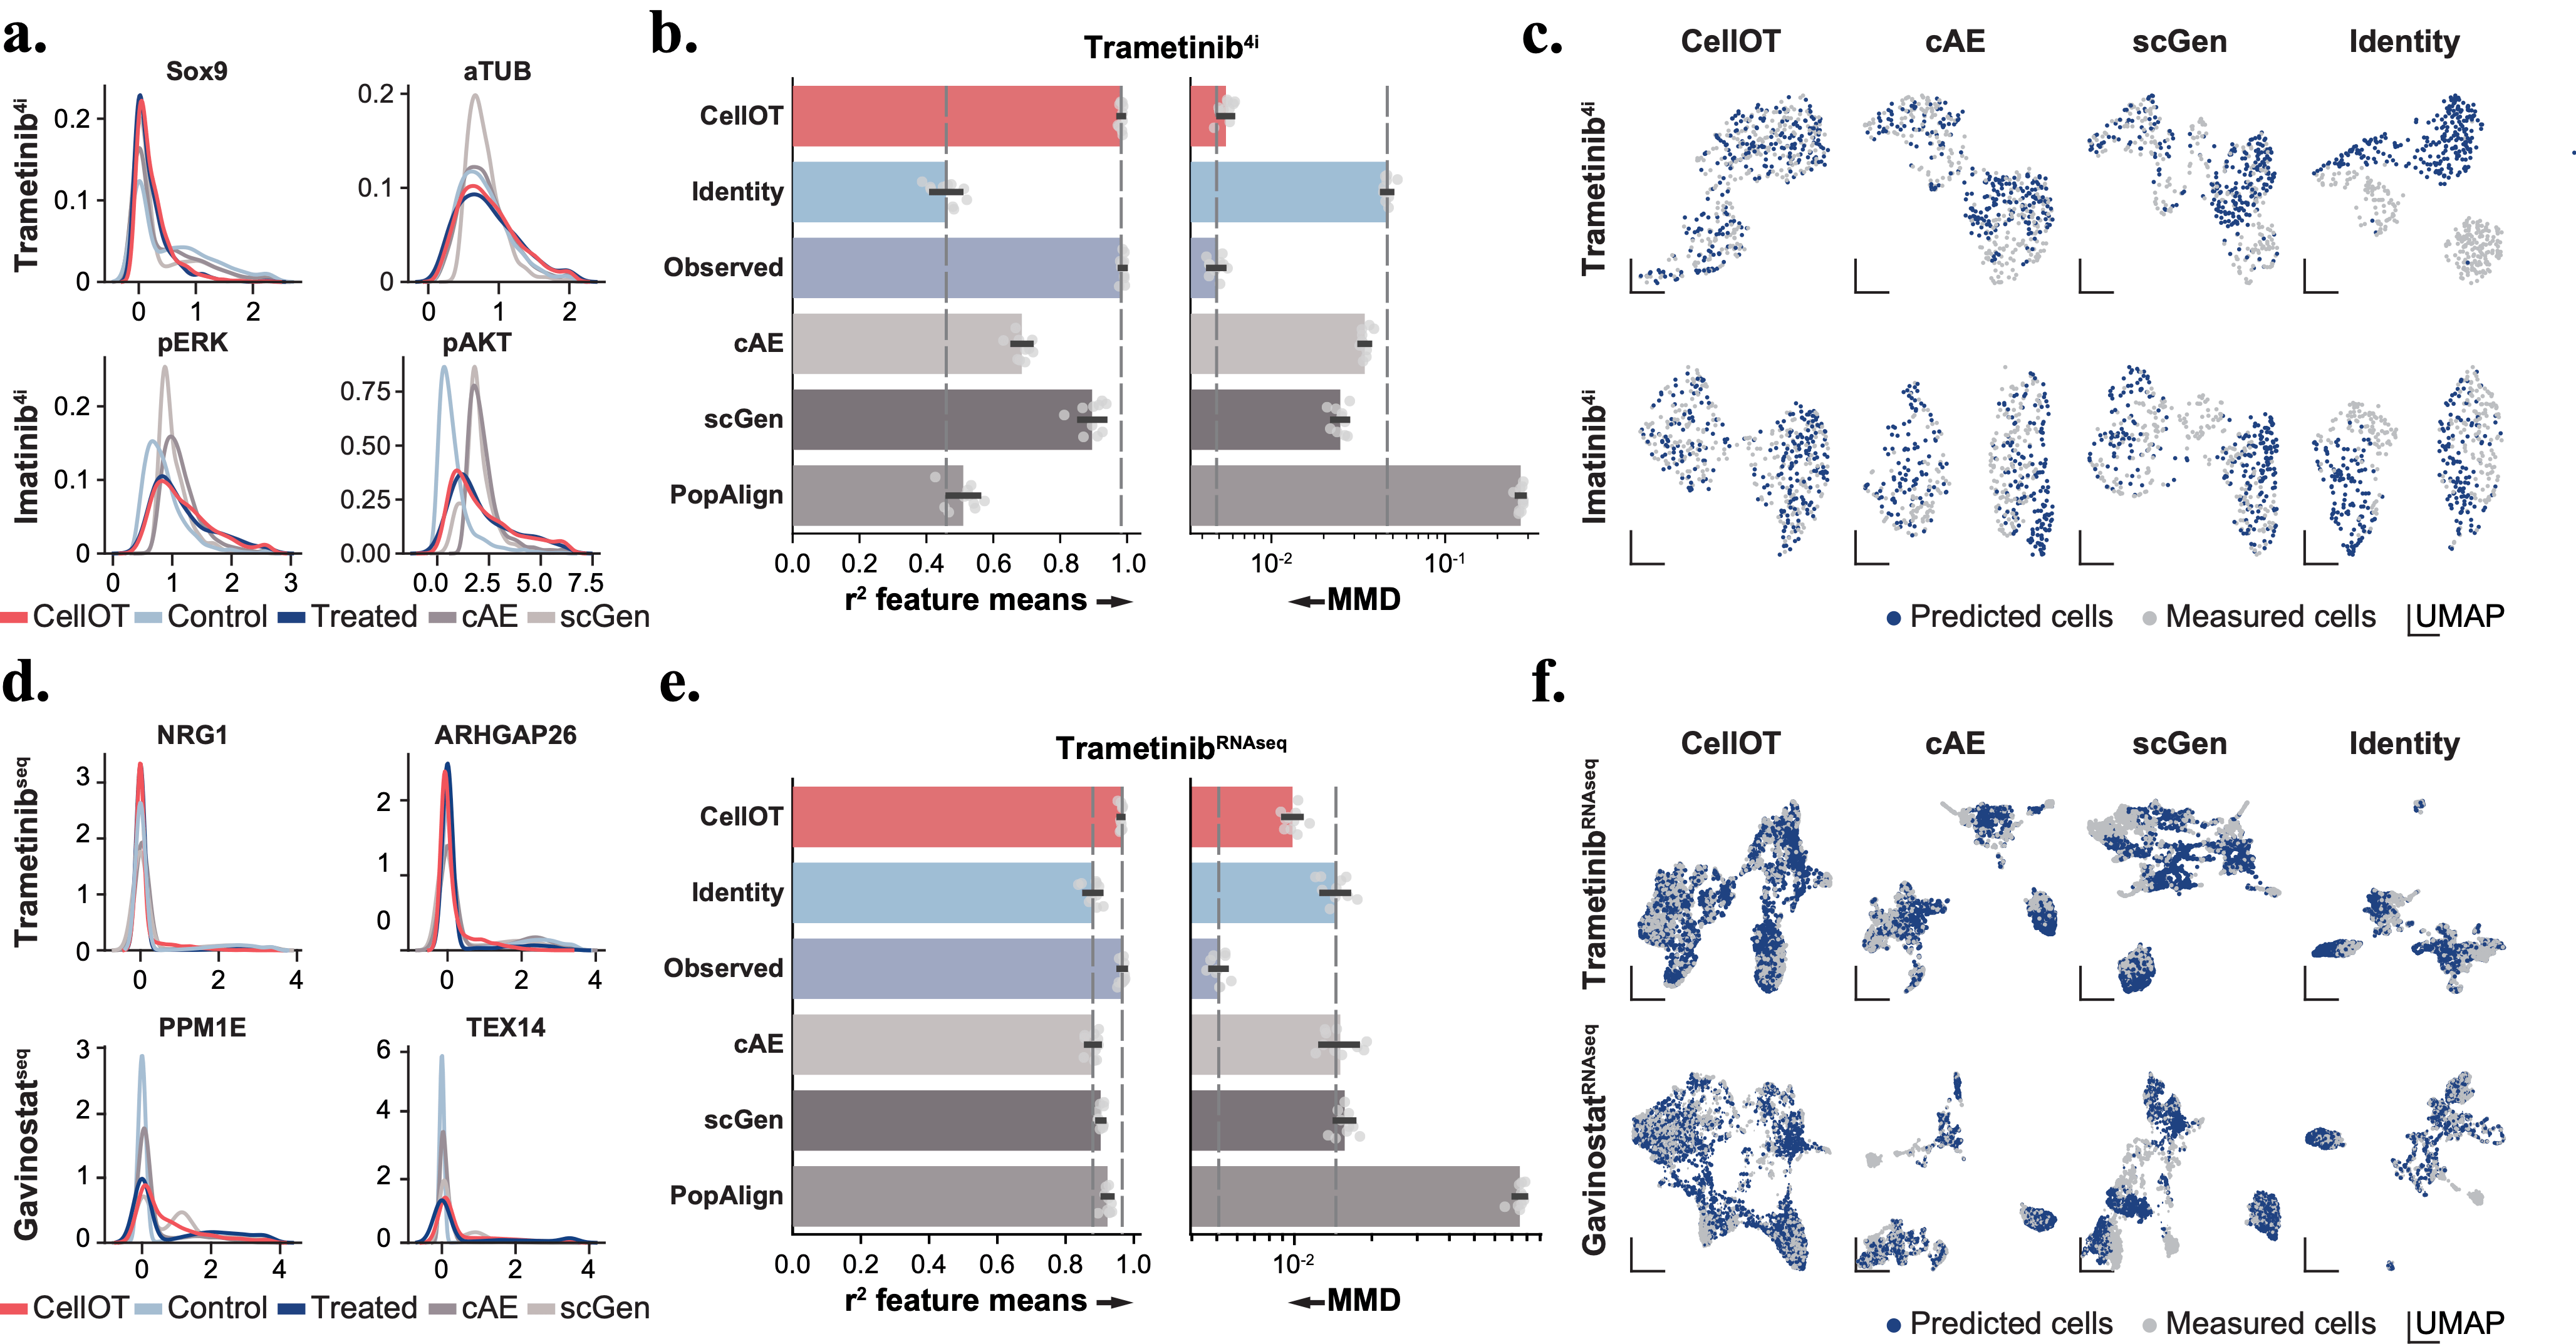
\includegraphics[width=\textwidth]{figures/fig_benchmark_cellot.pdf}
    \caption{\looseness -1 \textbf{\textsc{CellOT} outperforms current state-of-the-art methods on different data modalities.}  Marginal distribution of marker gene expression (x-axis) of cells profiled by \textbf{a.} 4i and \textbf{d.} scRNA. Observed control and treated states are shown in light and dark blue. \textsc{CellOT} predictions are shown in red and baseline predictions (scGen, cAE, PopAlign) are shown in gray. We compare models based on the distributional distance \acrshort{MMD} as well as average correlation coefficient $r^2$ between observed perturbed and predicted perturbed cells, for \textbf{b.} 4i and \textbf{e.} scRNA data. Error bars refer to the standard deviation over 10 bootstraps of the test set and the dashed lines correspond to the median of the identity and observed performances. Joint \acrshortpl{UMAP} of observed treated cells and cells predicted by each model for \textbf{c.} 4i and \textbf{f.} scRNA data. Projections are computed on a joint set of cells, down-sampled such that the number of observed perturbed (gray) and predicted perturbed cells (blue) are equal. An identity coupling compares treated cells to untreated cells. The analysis is conducted for the drugs Trametinib, Imatinib, and Gavinostat. 4i data was generated using cell lines M130219 and M130429.}
    \label{fig:benchmark_cellot}
\end{figure}
Optimal transport problems return the alignment between distributions $\mu$ and $\nu_k$ corresponding to the minimal overall cost between aligned molecular profiles, thus determining the most likely state of each cell upon perturbation (\cref{fig:overview_cellot}c).
$T_k$ is learned such that its image corresponds to $\nu_k$ and mass is moved from $\mu$ into $\nu_k$ according to a principle of minimal effort.
% Utilizing recent advancements in neural optimal transport theory, \textsc{CellOT} considers the dual form of the transport problem and parameterizes a pair of convex potentials with neural networks. $T_k$ is recovered as the gradient of one of these potentials.
As directly parameterizing the optimal transport map $T_k$ \citep{korotin2021wasserstein, yang2018scalable, prasad2020optimal} is unstable \citep[Table 1]{makkuva2020optimal}, we parameterize the convex potentials of the approximate semi-dual optimal transport problem $\varphi$ and $g$ \eqref{eq:ot-minmax}.
Given a set of perturbations $K$, and sample access to the control distribution $\mu$ as well as  distributions $\nu_k$ for each perturbation $k \in K$, \textsc{CellOT} learns the optimal pair of dual potentials $(\varphi_{\theta_k^\star}, g_{\phi_k^\star})$ by solving~\eqref{eq:cellot-optim}, each input convex neural networks \citep{amos2017input} is trained with loss functions \eqref{eq:makkuva_f_loss}-\eqref{eq:makkuva_f_loss}. We recover the optimal map $T_k$ using the gradient of a convex function $\varphi_k$, i.e., $\nabla \varphi_k$ \citep{makkuva2020optimal}.
% Using the learned convex potentials for each $k$, \textsc{CellOT} then predicts the transformation of a control cell $x_i$ upon perturbation $k$ via $\hat{y}_i^k = \nabla f_{\theta_k^\star}(x_i)$, i.e., samples following the predicted perturbed distribution $\hat{\nu_k} =(\nabla f_{\theta_k^\star})_{\sharp} \mu$. 

\section{Empirical Evaluation}

\subsection{Predicting Treatment Outcomes of Cancer Drugs}

\looseness -1 We apply \textsc{CellOT} to predict the responses of cell populations to cancer treatments using a proteomic dataset consisting of two melanoma cell lines (M130219 and M130429) \citep{raaijmakers2015new}, profiled by 4i~\citep{gut2018multiplexed}, and a scRNA-seq dataset~\citep{srivatsan2020massively}, which contain 34 and 9 different treatments, respectively.
% To put \textsc{CellOT}'s performance in perspective, we benchmark it against current state-of-the-art methods based on autoencoders \citep{lotfollahi2019scgen, lopez2018scvi}, which attempt to add perturbation effects through the manipulation of a learned latent representation.
We benchmarked \textsc{CellOT} against two autoencoder-based tools, \textsc{scGen}~\citep{lotfollahi2019scgen} and \textsc{cAE}~\citep{lopez2018scvi}, as well as \textsc{PopAlign}~\citep{chen2020dissecting}, a method based on aligning subpopulations of the control and treated space approximated through a mixture of Gaussian densities.
To further test the hypothesis of the optimal transport modeling prior, we compare the learned OT map $\nabla f_k$ for each perturbation $k$ with naive non-OT-based alignments.
Due to the high dimensional nature of scRNA-seq data, we apply $\textsc{CellOT}$ on latent representations learned by an autoencoder.
The marginal distributions for observed and predicted cell populations for two 4i treatments and two scRNA-seq treatments are shown in \cref{fig:benchmark_cellot}a, d. 
Two features are selected for each perturbation.
While the autoencoder baselines tend to capture the mean of the treated cell population, they are less successful in matching all heterogeneous states of the perturbed population, i.e., higher moments of the perturbed population.
% More precisely, these methods do not capture higher moments of the perturbed population, as for example the standard deviation of phosphorylated AKT (pAKT) levels of Imatinib-treated 4i cells. 
Thus, these models tend to learn over-simplified perturbation effects and are insufficient when aiming to understand heterogeneous rather than average cellular behaviors.
\textsc{CellOT}, on the other hand, is able to capture these higher moments, yielding accurate and nuanced predictions.

 \begin{figure}
     \centering
     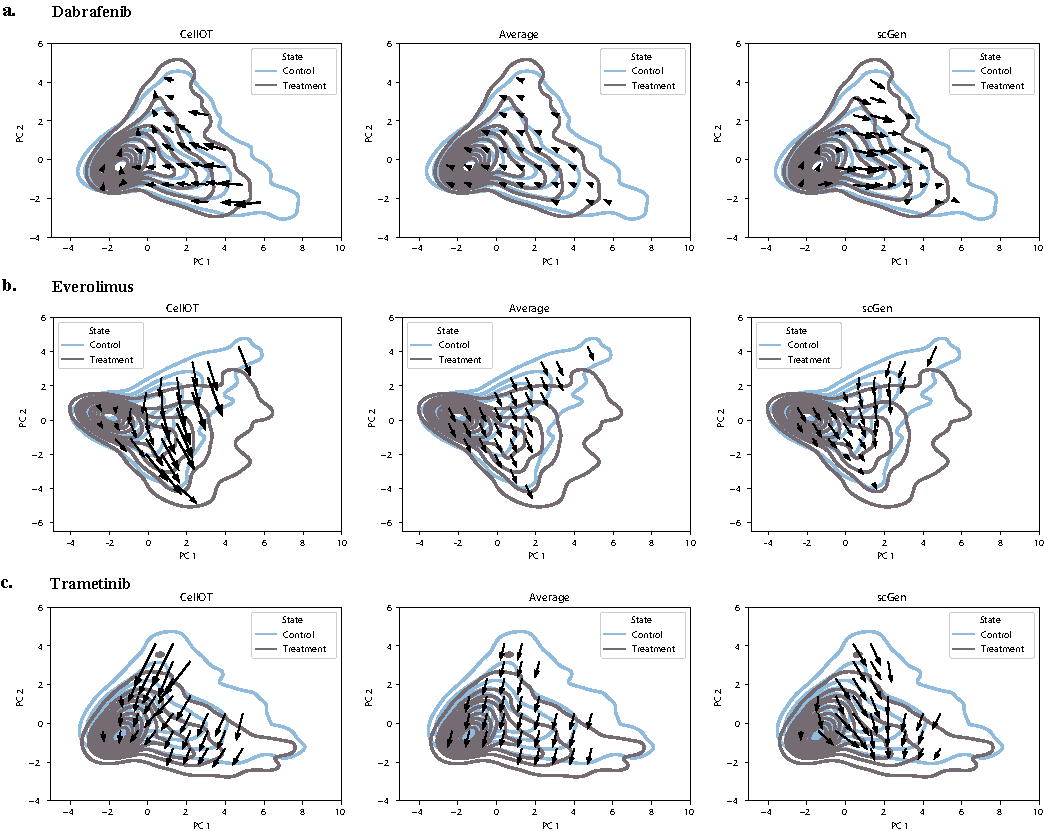
\includegraphics[width=\textwidth]{figures/fig_4i_vector_fields.pdf}
     \caption{Visualization of the learned vector field describing the perturbation response on the single-cell level for \textbf{a.} Dabrafenib, \textbf{b.} Everolimus, and \textbf{c.} Trametinib of the 4i dataset for \textsc{CellOT}, the average effect, and \textsc{scGen} on the first two principal components. Cellular responses are computed as the predicted treated state minus the observed control state for each individual cell. Arrow tails are placed in a grid within PC space and arrow heads correspond to the average response of cells within each neighborhood, projected into PC space.}
     \label{fig:4i_vector_fields}
 \end{figure}

\looseness -1 This can be further quantified % differences between the distributions of observed and predicted treated cell populations, we determine 
through distributional metrics such as the \acrfull{MMD} \citep{gretton2012kernel}.
Low values of \acrshort{MMD} imply that all moments of two distributions are matched, and thus the entire distribution of perturbed cells is captured in fine detail, beyond the population average.
The \acrshort{MMD}s between the predicted and observed populations for the selected perturbations are shown in \cref{fig:benchmark_cellot}b, e.
For scRNA-seq data, \acrshort{MMD} evaluations are computed using the top 50 marker genes.
In addition to the autoencoder baselines, we include the trivial \emph{identity} baseline that predicts treatment effects simply by returning the untreated states,
as well as a theoretical lower bound, \emph{observed}, comprising a different set of observed perturbed cells, thus only varying from the true predictions up to experimental noise.
We find that \textsc{CellOT} can approach the lower bound (\emph{observed} setting), while the baseline methods often do not improve much over the \emph{identity} setting.
Fig. \ref{fig:4i_vector_fields} visualizes the learned maps, % projected onto the first two principal components, 
further demonstrating \textsc{CellOT}'s ability to model fine-grained responses.


\looseness -1 Finally, we compute \acrfull{UMAP} projections~\citep{umap} on a joint set of predicted and observed perturbed cells utilizing the full feature space, shown in \cref{fig:benchmark_cellot}c, f.
We observe that the perturbed cell states inferred by \textsc{CellOT} are well integrated with the observed perturbed cells. Again, both baselines do not recover the perturbed distribution in its entirety % (via higher order moments)
and thus the perturbed state of different subpopulations is not captured consistently.
$\textsc{CellOT}$ outperforms the baselines in both metrics across all treatments, typically by one order of magnitude.
We attribute the strong performance of \textsc{CellOT} to its ability to learn a transport function that considers explicitly the data geometries of cell populations through the theory of optimal transport.

\subsection{Capturing Cell-to-Cell Variability in Drug Responses}
\looseness -1 Capturing distinct perturbation responses of different cell types within the same sample remains a challenging computational task. To reduce the task's complexity, prediction algorithms can be guided by predefined cell type labels both in the perturbed and unperturbed states \citep{chen2020dissecting} or set to approximate the mean drug response \citep{lotfollahi2019scgen}.  These simplifications come at a cost: the reliance on a priori knowledge about present and relevant cell types, the assumption that cell types are characterized by the same features before and after a perturbation, and that the drug response is uniform within a cell type.
In the worst case, these limitations risk masking true and important drug response heterogeneity  and thus hamper the discovery of novel cell types or cell state-specific perturbation responses.

\textsc{CellOT} is free of these limitations and enables scientists to query the predicted single-cell responses at the granularity best suited to answer their biological questions. As a proof of concept, we co-cultured the aforementioned patient-derived melanoma cell lines at equal ratios and performed a boutique drug screen, during which we exposed cells 8h to a panel of 34 drugs and measured the single-cell drug responses with the 4i technology. 
Using \textsc{CellOT}, 
% and cells from both cell lines, 
we predict the perturbed cell states of a shared set of control (DMSO-treated) cells (\cref{fig:biological_analysis}a) for each drug.
Previous work \citep{kramer2019cellular} shows that phosphorylation levels of signaling kinases upon drug treatments are tightly linked to the cellular state. 
To assess whether this relationship was retained in predicted compared to observed perturbed cells, we analyzed the phosphorylation levels of extracellular signal-regulated kinases (pERK) using the transport maps learned by \textsc{CellOT} on each drug.
Using 750 predicted and 750 observed perturbed cells, we computed \acrshort{UMAP} projections joint-wise from all features except pERK. \cref{fig:biological_analysis}b shows the predicted and observed population individually annotated with the respective pERK levels of each cell. We find the spatial organization of the two projections to look almost identical and that pERK levels had a highly comparable distribution across the cells of either class and all drug treatments (further analysis in \cref{fig:4i_analysis_extended}a, b).
% We furthermore supplemented this analysis by faithfully reconstructing unseen pERK levels of predicted cells from their local neighborhoods in multidimensional feature space

% Based on the 3 nearest neighbors computed using all features except pERK, we show that these features of importance are faithfully reconstructed by observed cells in the local neighborhood of each predicted cell, thus, retaining the crucial connection between kinase activity levels and cellular states.

% \subsection*{\textsc{CellOT} enables cell state-aware drug profiling and disentangles subpopulation-specific drug effects}
\subsection{Disentangles Subpopulation-Specific Drug Effects}
\textsc{CellOT} allows us to 
% profile the severity of drug perturbations on individual cellular states and understand how the cellular state of unperturbed cells determines drug response behavior. We can 
isolate the mode of action of each drug by computing the difference between predicted perturbed cells and untreated control cells. % , i.e., the \emph{cost} of the optimal transport.
A \acrshort{UMAP} embedding of all cells color-coded by the treatment distinctly separates different treatments (Figs.~\ref{fig:biological_analysis}c and \ref{fig:4i_analysis_extended}e), all of which \textsc{CellOT} is able to faithfully learn.
Such distinct treatment embeddings are not present when accounting only for an average perturbation effect (\cref{fig:4i_analysis_extended}d), indicating the importance of capturing the cellular heterogeneity of drug responses.

\looseness -1 Using Leiden clustering on the full feature set, we grouped unperturbed control cells in 12 cellular states (\cref{fig:biological_analysis}d, \cref{fig:4i_analysis_extended}g). Cellular states 1, 5, 6, 9, and 12 show high levels of MelA and no SOX9 and thus correspond to the melanocytic cell line M130429, whereas the SOX9\textsuperscript{+} and MelA\textsuperscript{-} states 2, 3, 4, 7, 8, 10, and 11 represent the mesenchymal cell line M130219. Overall, we find that M130429 cells have higher phosphorylation levels of the measured signaling kinases compared to M130219;
% The cluster structure derived from the control cells is further persistent in the perturbed states. 
a stereotypical spatial organization of cellular states is retained for the majority of the drugs,  and cell states belonging to the same cell line cluster together (\cref{fig:4i_analysis_extended}f). 

\begin{figure}
    \centering
    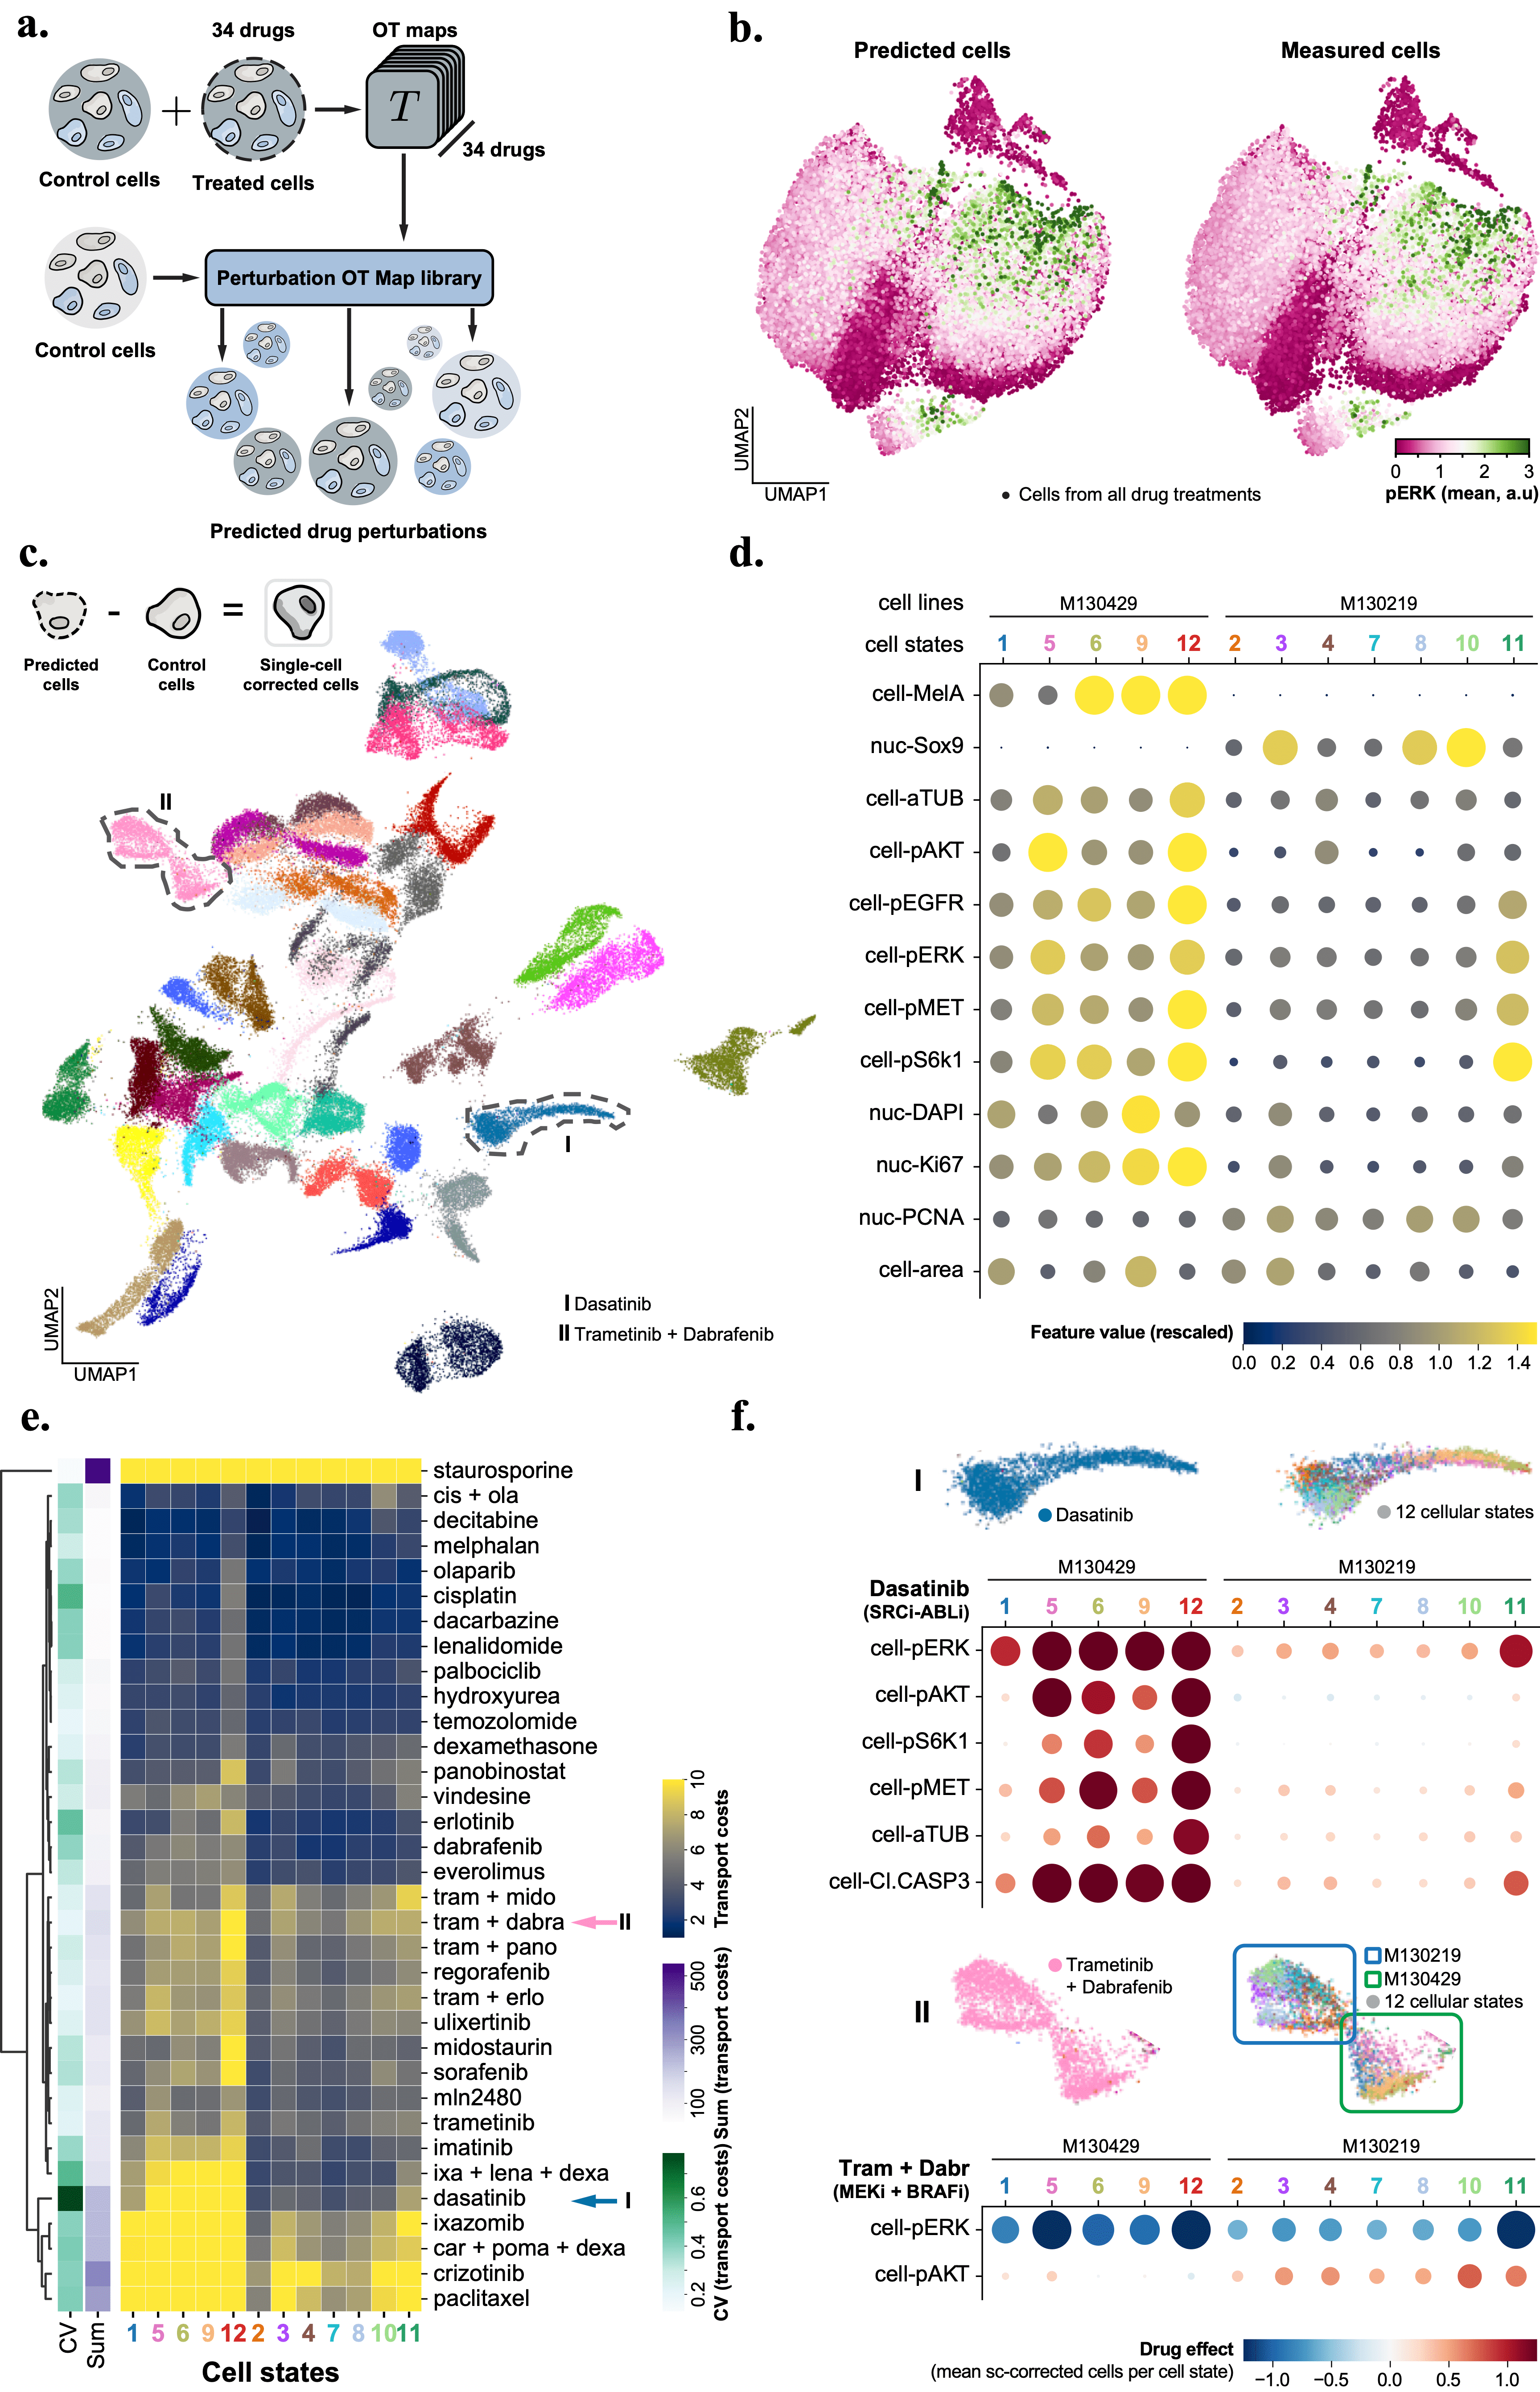
\includegraphics[width=\textwidth]{figures/fig_biological_analysis.pdf}
\end{figure}
\captionof{figure}{
\looseness -1 \textbf{CellOT facilitates the multiplexed single-cell characterization of cancer drugs.} 
    \textbf{a.} \textsc{CellOT} training and prediction setup. 34 \textsc{CellOT} models were trained, one for each drug perturbation. Subsequently, each model was used to predict perturbed cells from a common set of unseen control cells. \textbf{b.} \acrshort{UMAP} projection constructed with equal numbers of predicted and measured cells from 34 perturbations. Dots correspond to cells, color-coded for measured or predicted pERK intensity, \textbf{c.} \acrshort{UMAP} projection of single-cell perturbation effects using predicted cells. Dots correspond to cells, color-coded for drug treatment (see \cref{fig:4i_analysis_extended} for a full legend for single-cell perturbation effect calculation). \textbf{d.} Cell states identified in control cells. Each column represents a cell state. Horizontal axis, cell states are sorted based on their association with the cell lines M130219 and M130429.  Vertical axis, cellular features (see \cref{fig:4i_analysis_extended} for the full feature set). The size and hue of the circles are scaled on the feature values. \textbf{e.} Clustergram of transport cost (TC) of drug treatments for each cell state (main heatmap, blue-yellow color scheme), the sum of TCs (Sum) of all states per drug (first column left of the heatmap, purple), the coefficient of variation (CV) of TCs per drug (second column left of the heatmap, green) and the dendrogram based on the hierarchical clustering the drug's cell state TCs. Cell states are sorted as in \textbf{d}. \textbf{f.} Cell state-specific responses to drug treatments. Top panel (I) Dasatinib. Bottom panel (II) Trametinib + Dabrafenib. Panel organization: top-left, condition-focused enlargement of \acrshort{UMAP} projection from \textbf{c}. Top-right, same as top-left but color-coded for cell state assignment. Bottom, columns represent a cell state,  rows highlighted features. `cell-' stands for mean cell intensity. Circles are scaled based on drug effect size, the stronger the effect the larger the circles. Negative values are encoded in hues of blue, and positive values in red hues of the respective circles. \vspace{10pt}}
\label{fig:biological_analysis}
\looseness -1 Computing the difference between the control and treated state of each drug, i.e., the optimal
% what corresponds to the 
transport cost, allows us to further characterize a drug's severity. 
% High overall transport costs correspond to large feature value changes, i.e., a strong perturbation effect. 
Apoptosis inducers (e.g., Staurosporine), proteasome inhibitors (e.g., Ixazomig and Carfilzomib or the combination treatment Carfilzomib + Pomalidomide + Dexamethasone), microtubule-stabilizing agents (e.g., Paclitaxel), c-Met inhibitors (e.g., Crizotinib), and ATP competitors for multiple tyrosine kinases such as c-KIT, and Bcr-Abl (i.e., Dasatinib) show high transport costs and thus substantial feature changes in all cellular states (\cref{fig:biological_analysis}e). Other drugs demonstrate less severe effects in the observed 8h incubation period. 
% Nonetheless, we find that most  drugs affect multiple cellular states and that individual cellular states have varying sensitivities to drugs in the drug panel.
We find all perturbations to increase levels of cleaved Caspase 3, an apoptosis marker, in various cellular states and in both cell lines (\cref{fig:4i_analysis_extended}k), with the exception of Dasatinib, which specifically induced cell death in cellular states 5, 6, 9, and 19 associated to M130429 (\cref{fig:biological_analysis}f).


\looseness -1 Previous work by \citet{smith2016inhibiting} reports that M130429 cells reduce metabolic activity % (a proxy of cell viability)
upon treatment with inhibitors of MEK (MEKi) and RAF (RAFi), while M130219 cells are resistant to these inhibitors. When comparing the responses of the two cell lines to Trametinib (MEKi) and MLN2480 (panRAFi) in the MEK and PI3K pathway using pERK and pAKT as the respective readouts, we find that MEKi-sensitive M130429 cells down-regulate pAKT and pERK, whereas the MEKi-resistant M130219 cells only down-regulate pERK. Consistently, we also find that treatment with MLN2480 results in a similar differential drug response (\cref{fig:4i_analysis_extended}i). This suggests that \textit{decoupling} of the MEK and PI3K pathways may confer resistance to MEK and Raf inhibitors and constitute an adaptation to the escape of cancer therapy \citep{kun2021mek}. We find further supporting evidence of pathway crosstalk alteration when we analyze pAKT and pERK levels upon treatment with a cocktail of Trametinib (MEKi) and Dabrafenib (BRAFi). 

\looseness -1 In response to two drugs impinging on the MEK pathway, we observe pERK to be reduced in both cell lines but increased pAKT levels in the MEKi-resistant cell line M130219 (which resistance was acquired during pre-exposing a patient to MEKi) (\cref{fig:biological_analysis}f). This finding points towards a compensatory feedback mechanism acquired by M130219 during MEKi treatment by which inhibition of the MEK pathway (quantified as a reduction of pERK) would stimulate signaling through the PI3K pathway, possibly through activation of an upstream receptor kinase \citep{caunt2015mek1}. 
Our results on two co-cultured primary melanoma cell lines treated with various anti-cancer drugs show that \textsc{CellOT} can accurately capture phenotypic heterogeneity in unperturbed cell populations and predict diverse drug responses by incorporating the underlying cell-to-cell variability without predefined cell line labels. 
% Further, we find that \textsc{CellOT} reveals differential drug responses between the cellular states of the same cell lines, thus showcasing its ability to reveal unknown cell state-associated drug responses in an unsupervised fashion.
    
% \subsection*{\textsc{CellOT} accurately predicts single-cell responses for unseen patients}
\subsection{Inferring Cellular Responses in Unseen Patients}
The maps between molecular states before and after treatments learned by \textsc{CellOT} contribute to a better understanding of the differences between cells that respond to certain drugs and cells that do not respond. This is crucial for inferring an incoming patient's response to drugs and settings with high cell-to-cell variability.
To make predictions on unseen patients, however, we need to demonstrate that the learned maps $T$ model perturbation responses across different patients coherently and robustly, while still predicting personalized treatment outcomes for each patient instead of mere population averages.

% TODO: Check acronyms.
To test the generalization capacity of \textsc{CellOT} in such an \acrfull{oos} scenario, we use a \acrfull{PBMC} droplet scRNA-seq dataset. \citet{kang2018multiplexed} characterize the cell type specificity and inter-individual variability of the response of eight lupus patients to interferon beta (IFN-$\beta$), a potent cytokine that induces genome-scale changes in immune cell transcriptional profiles. 
% The dataset contains two pools, IFN-$\beta$-treated and control, prepared with the same number of cells from each individual, thus allowing us to investigate the cell fate differences between unperturbed and perturbed cells.
In the following, we compare the performance of \textsc{CellOT} and other baselines in an \acrfull{iid} setting, where models see cells from all patients, as well as in the out-of-sample setting, where models do not see cells from a specific holdout patient (see \cref{fig:generalization_cellot}a).
% A robust method should show little to no performance drop from the i.i.d. to the o.o.s. scenario.
    
As in the previous analysis, we evaluate how accurately \textsc{CellOT} captures the change in the overall expression of different marker genes from control to IFN-$\beta$-treated cells and thus how well the predicted gene expression marginals are aligned with the treated population (\cref{fig:generalization_cellot}b). Here, we consider the genes \textit{CXCL11}, \textit{CCL2}, and \textit{APOBEC3A},
since they are connected with autoimmune diseases, including systemic lupus erythematosus \citep{hedrich2011epigenetic, perez2021sustained}
and thus potential therapeutic targets
in the management of patients with lupus and, likely, other interferonopathies \citep{mathian2015targeting,rani1996characterization,hedrich2011epigenetic,mathian2015targeting,perez2021sustained,flier2001differential}.
% CXCL11 and CCL2 are both chemokines
These selected genes show a large change in expression from the control to the perturbed population, partially exhibiting a bimodal gene expression profile upon perturbation. In contrast to \textsc{CellOT}, the baselines do not accurately predict these large transcriptomic shifts of these genes.


\looseness -1 All models, including \textsc{CellOT}, show little performance drop when modeling the treatment outcome on a new patient using the generalized perturbation model $T_L$ trained on the patient cohort and using the control cells $\mu_z$ of the unseen patient as input.
This becomes evident when comparing the predicted population $\hat{\nu}_z$ with observations $\nu_z$ using the \acrshort{MMD} metric. \cref{fig:generalization_cellot}c displays summary results in which each individual patient was considered for the holdout set. \textsc{CellOT} outperforms previous baselines both in the i.i.d.~and in the o.o.s.~setting, while further showing a smaller performance drop when generalizing to the unseen patient.
These results suggest that the learned optimal transport maps correctly model the shift in the structures of the cellular subpopulation present in all patients, thus robustly performing out-of-sample.
We repeat the same evaluation for a glioblastoma cohort consisting of seven patients \citep{zhao2021deconvolution}. However, generalization within this setting proved to be difficult for \textsc{CellOT} and all baselines, due to the small size of the cohort and high degree of variance within the responses of each individual. 
% We have identified under which conditions generalization to unseen patients is feasible. 
For a complete analysis, see \cref{fig:gbm_patients_iid_ood}.

\begin{figure}
    \centering
    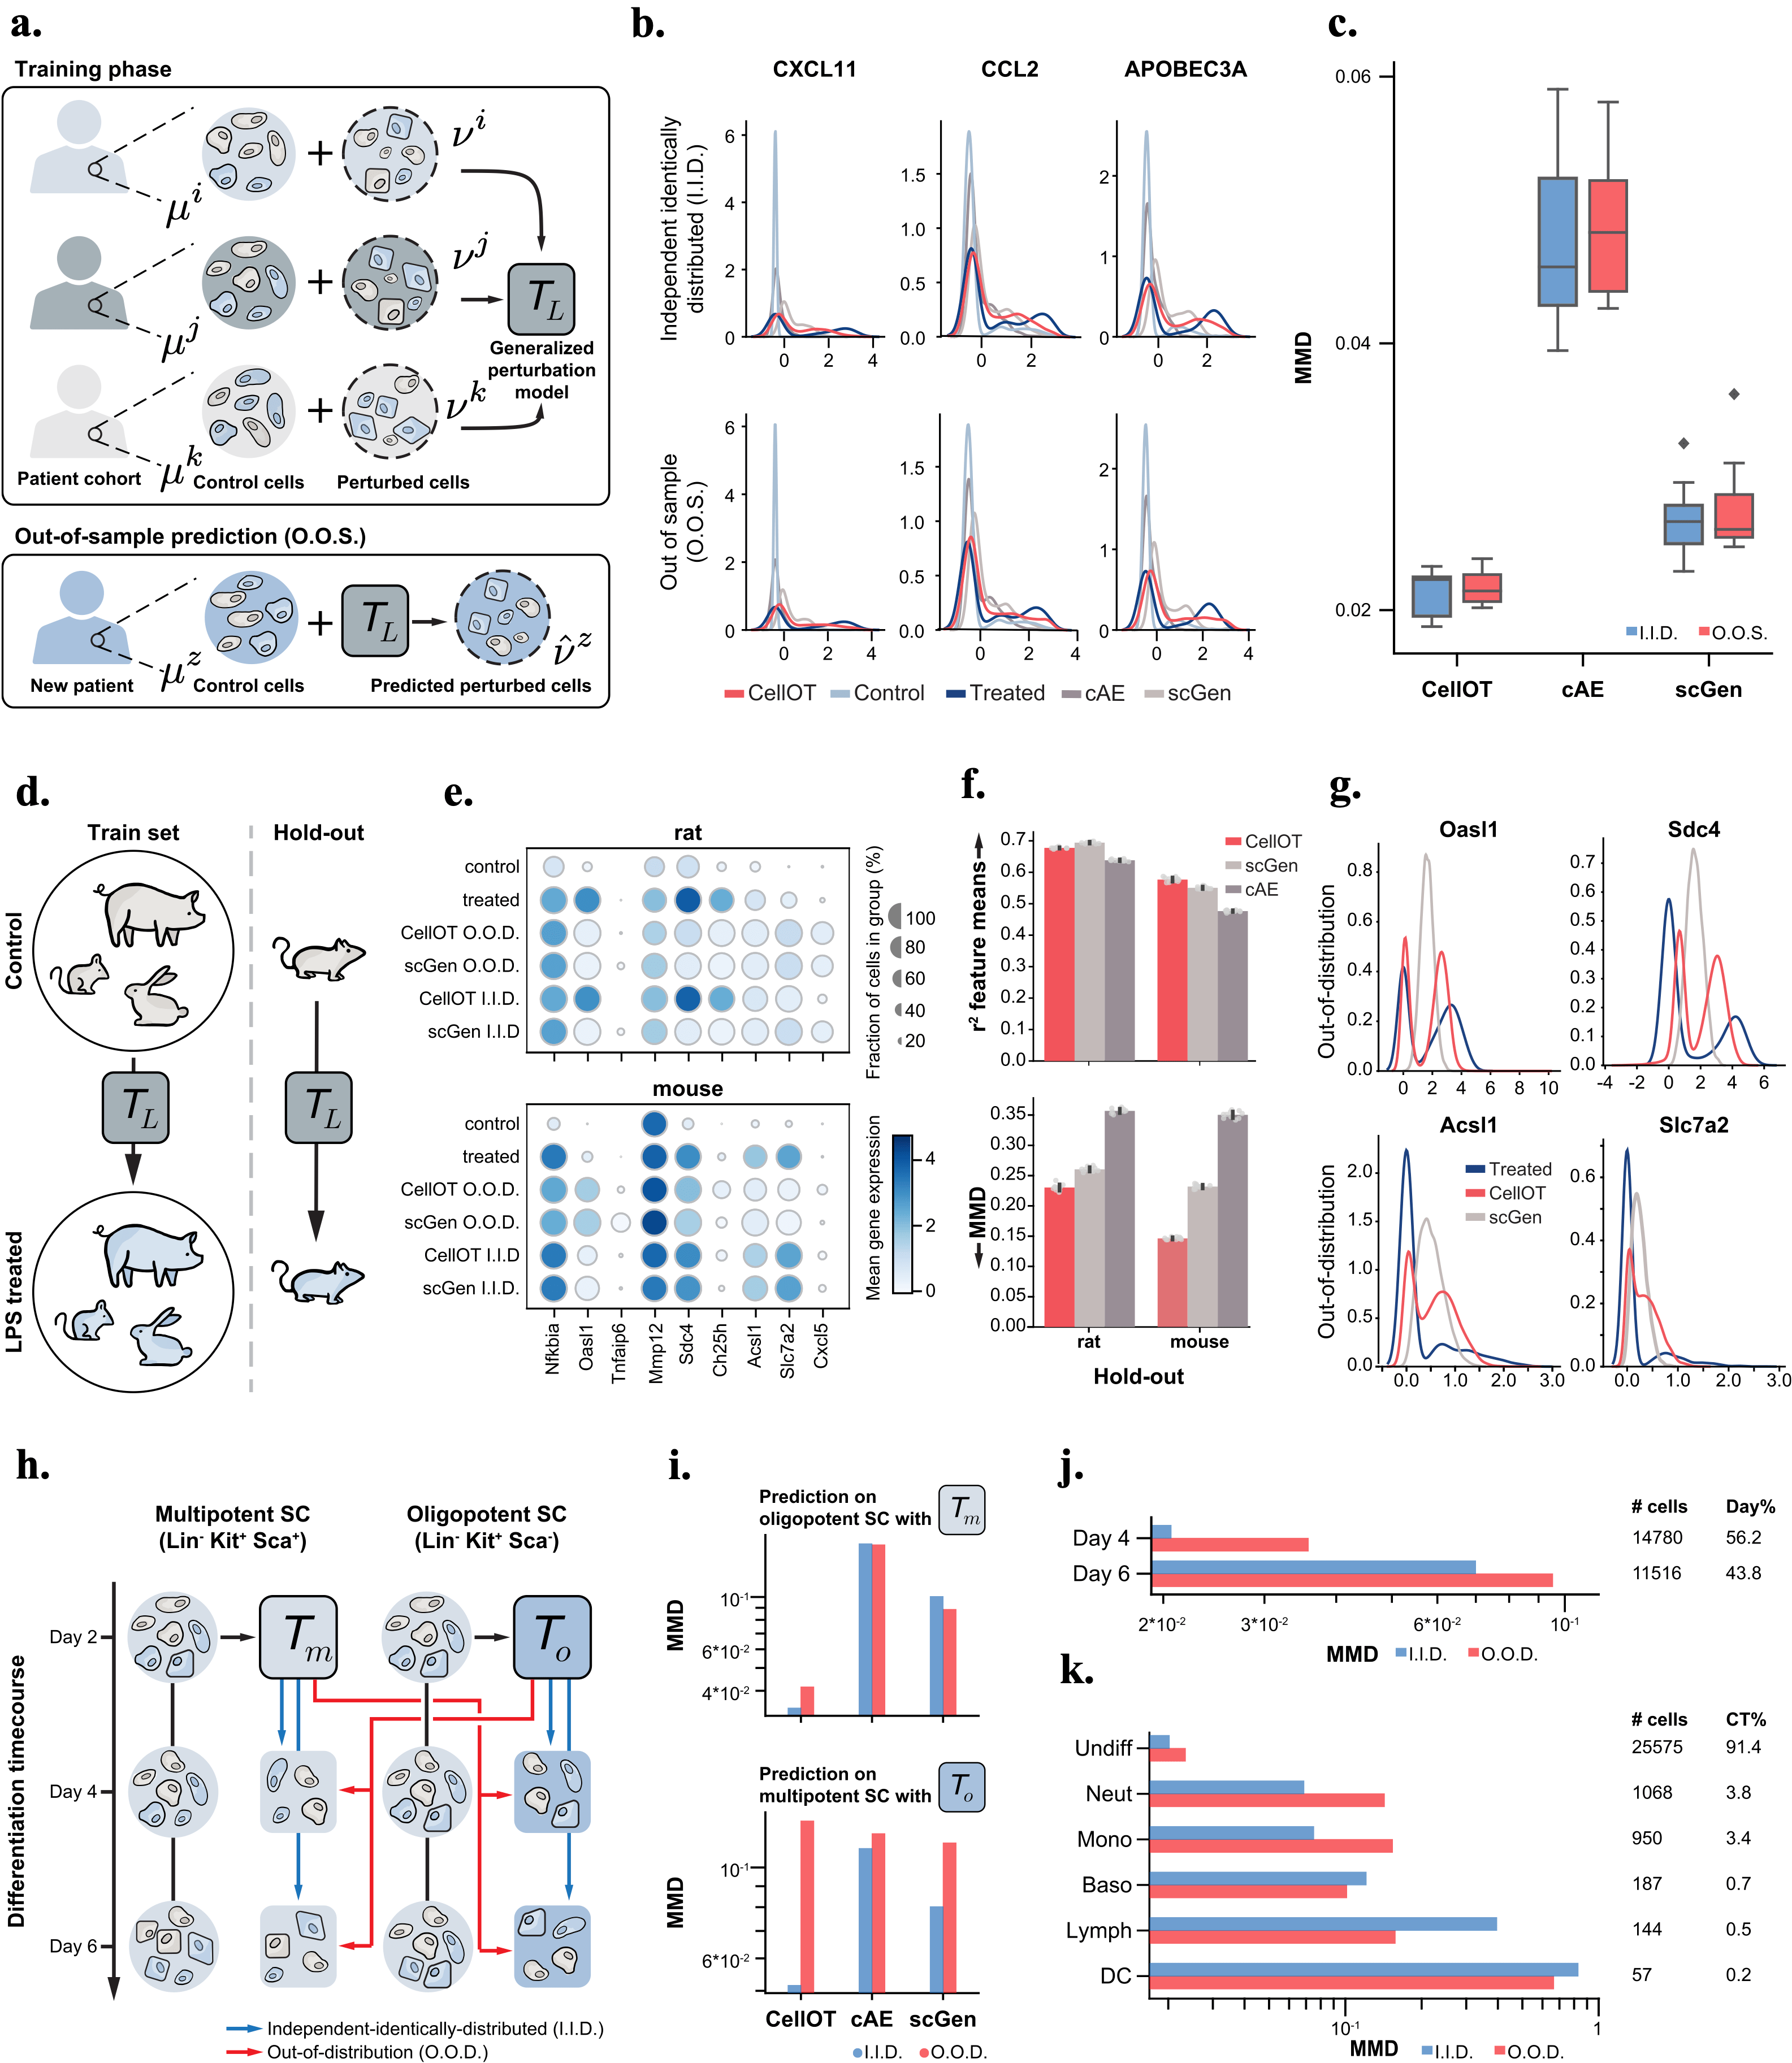
\includegraphics[width=1.05\textwidth]{figures/fig_generalization_cellot.pdf}
 \end{figure}
 \captionof{figure}{
    \textbf{\textsc{CellOT} generalizes to unseen patients and cell subpopulations.} Out-of-sample (o.o.s., \textbf{a-c}), and \acrlong{ood} (\acrshort{ood}, \textbf{d-k}) setting. \textbf{a.} Cells from eight lupus patients are measured in an untreated and IFN-$\beta$ treated state. 
%    For each sample, we train two models, an o.o.s.~model trained on cells from all other samples and an i.i.d.~model trained with additional access to half of the cells in the holdout sample (not shown). 
    \textbf{b.} Marginals of predicted cells from the holdout sample in the i.i.d.~(top) and o.o.s.~(bottom) setting. Predictions for both models are made on the same test set (not used for training the two models). \textbf{c.} \acrshort{MMD} scores between the predicted distribution and the observed treated distribution across all holdout samples in the i.i.d.~and o.o.s.~settings. Box plots indicate the median and quartiles.
    \textbf{d.} As an \acrshort{ood} task, we train \textsc{CellOT} and baselines to predict the response to LPS across different species, and test on rat (or mouse) as a holdout species. \textbf{e.} Mean gene expression for i.i.d. and \acrshort{ood} predictions for \textsc{CellOT} and \textsc{scGen} for selected marker genes.  \textbf{f.} Comparison of \acrshort{ood} performance for $r^2$ correlation feature means and \acrshort{MMD} of \textsc{CellOT} and baselines. Data are depicted as the mean +/- standard deviation across n=10 bootstraps of the test set. \textbf{g.} Marginals of the \acrshort{ood} predictions for marker genes showing bimodal expression profiles when using rat as a holdout.
    \textbf{h.} We apply \textsc{CellOT} to predict how cells from day 2 develop into the combined set of day 4 and 6 when trained on only multipotent cells ($T_m$) or oligopotent cells ($T_o$). We then apply $T_m$ to predict the \acrshort{ood}~oligopotent cells and $T_o$ to predict the \acrshort{ood}~multipotent cells. \textbf{i.} \acrshort{MMD} scores between the predicted and (observed) developed distributions for all models in both \acrshort{ood}~ and i.i.d.~prediction tasks (jointly for day 4 and 6). Performance of \textsc{CellOT}, when predicting \textbf{j.} day 4 states and day 6 states \textbf{k.} for different cell types in each setting using $T_m$. \vspace{10pt}}
    \label{fig:generalization_cellot}

\subsection{Reconstructing Innate Immune Responses across Different Species}
%\subsection{\textsc{CellOT} reconstructs innate immune responses across species}

The innate immune response is a cell-intrinsic defense program showing high levels of heterogeneity among responding cells and thus an ideal task for evaluating \textsc{CellOT}'s capabilities. We rely our analysis on the dataset collected by \citet{hagai2018gene}, which studies the evolution of innate immunity programs of mononuclear phagocytes within different species, including pigs, rabbits, mice, and rats. For this, these primary bone marrow-derived cells are stimulated using \acrshort{LPS}.
In the following, we test how well \textsc{CellOT} and the baselines reconstruct innate immune responses within species that are not encountered during training. We refer to the generalization task as \acrfull{ood}, since unlike the o.o.s.~setting, we expect different species to have very distinct responses (see \cref{fig:generalization_cellot}d).
The holdout set thereby consists of cells derived from either rat or mouse. See \cref{fig:crossspecies_ood_analysis}a,b for an analysis of cross-species similarity and the reasoning behind selecting the holdout set.

Indeed, \textsc{CellOT} accurately reconstructs the innate immune response in both mouse and rat in the i.i.d. and \acrshort{ood} setting. This not only becomes evident through capturing more precisely the mean expression level of marker genes that show high differential expression levels upon addition of \acrshort{LPS}, e.g., \textit{Nfkb1} (NF-$\kappa$B), \textit{Oasl1} (Oasl1), \textit{Mmp12}, and \textit{Cxcl5} (see Figs.~\ref{fig:generalization_cellot}e and \ref{fig:crossspecies_ood_analysis}c-d), but also through the average correlation coefficient $r^2$ computed between \acrshort{ood} predictions and holdout observations across all genes (see \cref{fig:generalization_cellot}f).
In particular, \textsc{CellOT} outperforms the baselines when analyzing how well each method captures the heterogeneity of innate immune responses in different species, as demonstrated by low levels of \acrshort{MMD} (see \cref{fig:generalization_cellot}f).
Most impressively, our method shows a strong alignment or gene expression marginals of aforementioned marker genes that show complicated bimodal expression profiles upon perturbation (see \cref{fig:generalization_cellot}g).

% \subsection*{\textsc{CellOT} generalizes perturbation responses \acrlong{ood} from multipotent populations to cells of lower potency}
\subsection{Generalizing Developmental Fate Decisions from Multipotent to Oligopotent Cell Populations}

\looseness -1 During developmental processes, stem and progenitor cells progress through a hierarchy of fate decisions, marked by a continuous differentiation of cells that refine their identity until reaching a functional end state.
% Modern high-throughput methods allow us to monitor these successive changes in gene expression profiles by observing multiple snapshots over time. To ultimately associate molecular differences among progenitor cells with their capacity to generate mature cell types and get a better understanding of biological differentiation or reprogramming mechanisms, we are required to learn the alignment of progenitor to mature cell states.
By tracking an initial cell population along the differentiation process, \textsc{CellOT} allows us to recover individual molecular cell fate decisions and developmental trajectories. 
% Here, the perturbation of the control population of progenitor cells is initiated by internal molecular factors driving developmental processes instead of some external factor. 

% \citet{weinreb2020lineage} use the mouse hematopoietic system as a model for a developmental process. To be able to clonally trace transcriptomes over time and capture not only each transcriptional cell state but also fate, each cell contains a genetic barcode that remains throughout cell division. This not only allows one to detect sister cells in the earliest stages of the developmental process but also links differentiated cells sampled at a later stage of the differentiation process to the original cell by reading out the barcode.

\citet{weinreb2020lineage} analyzed the fate potential of \acrfull{HSPC}, by tracking a broad class of oligopotent %(LIN$^{-}$KIT$^{+}$SCA$^{-}$) 
and multipotent %(LIN$^{-}$KIT$^{+}$SCA$^{+}$)
 progenitor cell subpopulations and observing samples on days 2, 4, and 6 (\cref{fig:generalization_cellot}h).
Here, we test how well \textsc{CellOT} and other baselines can learn the differentiation process of the cells observed on day 2 to the cells observed on days 4 and 6 (combined) and generalize from one subpopulation to another (\acrshort{ood} setting).
% Similar to the o.o.s. setting, we train two models per subpopulation.
We learn two maps, where map $T_o$ is trained exclusively on oligopotent cells, and $T_m$ on multipotent cells.
I.i.d.~versions of these maps are trained on both oligopotent and multipotent cells, such that each pair of i.i.d.~and \acrshort{ood}~maps is evaluated on the same test set.
Comparing the distributional distance between predicted and observed differentiated cell states using the \acrshort{MMD} metric, \textsc{CellOT} outperforms current state-of-the-art methods in this i.i.d.~setting for both the oligopotent and the multipotent subsets (see \cref{fig:generalization_cellot}i).
Furthermore, while baselines struggle to perform in either \acrshort{ood}~setting, \textsc{CellOT} is able to generalize its predictions in one direction, i.e., from multipotent cells to the oligopotent setting.
In contrast to oligopotent cells, multipotent cells have a higher potency and thus can potentially differentiate into more cell types, and so we would expect $T_m$ is more likely to generalize than $T_o$, trained on the less potent oligopotent cells.
When predicting developmental perturbations on multipotent cells using $T_o$, the differentiated cell fates cannot be recovered.
% For this task, the overall performance of other chosen baselines is low and equivalent to a random shift. Here, both cAE \citep{lopez2018scvi} and scGen \citep{lotfollahi2019scgen} simply predict a random shift without biological meaning.
% , at a level at which the \acrshort{MMD} metric is no longer sensitive.

\looseness -1 
% Depending on shared or individual receptors, signaling pathways, and regulatory networks, the response to perturbations and sensitivity to developmental factors or drugs might vary strongly between cell types or at different points in time.
% However, a robust perturbation model is required to capture the perturbation response across different cell types as well as at various levels of temporal resolutions.
We further compare the performance at different time points and across cell types.
% The transportation maps $T_o$ and $T_m$ were trained to learn the response from day 2 cells to day 4 and 6 together (\cref{fig:generalization_cellot}h). 
\cref{fig:generalization_cellot}j shows the accuracy of the modeled development of multipotent cells using map $T_m$ individually for day 4 and day 6 cells, respectively. It is evident that \textsc{CellOT} achieves better results when predicting developmental dynamics short-range instead of states further away in time.
This suggests a potential limitation for all of these methods, which might be unable to recover alignments over coarse time resolutions.
% In addition, we further decompose the analysis to capture \textsc{CellOT}'s consistency across different cell types. 
Beyond, while the vast majority of cells on days 4 and 6 are still undifferentiated (undiff), some cells have evolved into neutrophils (neut), monocytes (mono), basophils (baso), lymphoid precursors (lymph), or dendritic cells (DC).
As expected, the performance of \textsc{CellOT} drops in terms of the \acrshort{MMD} metric for those cell types that are only sparsely represented in the dataset (see \cref{fig:generalization_cellot}k).

\section{Discussion}

Single-cell expression profiling provides a detailed look into the molecular states of individual cells, but it is destructive and does thus not allow continuous measurements of molecular properties over time. There have been numerous proposals for methods to uncover the dynamics of individual cells from population data, but all of them face the same challenge: sequentially observed distribution of cell states can be produced by multiple dynamics and mechanisms of gene regulation. The ill-defined nature of the problem makes it necessary to pose certain assumptions on the underlying cellular dynamics.

The mathematical foundation of this work builds on the biological intuition that perturbations incrementally alter the molecular profiles of cells. This principle aligns with the theory of optimal transport and, following previous work \citep{schiebinger2019optimal}, serves naturally as the model foundation of \textsc{CellOT}.
If this principle is violated, however, and perturbations strongly disrupt the population to an unidentifiable level, the performance of \textsc{CellOT} as well as other methods drops (see Discussion).
In these instances, more complicated mathematical machinery would be needed.
Such tools, however, are currently unable to scale to settings with more than a few genes \citep{heydari2022iqcell}.
Thus, we rely on a fine granularity of the time course to recover large cell state changes between consecutive time points \citep{tritschler2019concepts}.

Furthermore, if a system exhibits rotations and oscillations within two consecutive snapshots not captured by measurements, models based on optimal transport and previous tools \citep{weinreb2018fundamental} will not be able to recover such complex dynamics. This is in part also due to the current choice of the cost function, which, due to theoretical constraints and practical performance, is set to the Euclidean distance. We leave it to future work, to investigate choices of alternative cost functions. 

Beyond, the current system is not able to recover effects (other than cell flux) that change the distribution of cells between time points, for example, proliferation and death \citep{tritschler2019concepts}. Recent works propose extensions to the classical neural optimal transport scheme that account for cell death and birth \citep{lubeck2022neural}.

Lastly, current developments in bioengineering aim at overcoming the technological limitation of destructive cell assays. \citet{chen2022live} propose a transcriptome profiling approach that preserves cell viability. \citet{weinreb2020lineage} capture cell differentiation processes while clonally connecting cells and their progenitors through barcodes. These methods thus offer (lower-throughput) insights that provide individual trajectories of cells over time, i.e., an alignment between distinct measurement snapshots.
\citet{somnath2023aligned} propose a novel algorithmic framework connected to optimal transport that is able to make use of such (partially) aligned datasets \citep{shi2023diffusion, tong2023conditional}. 

\chapter{Neural Optimal Transport with Context}
\label{cha:condot}

\dictum[Stefan Zweig, \textit{Verwirrung der Gef{\"u}hle} (1927)]{%
  Auch die Pause geh{\"o}rt zur Musik.}%
\vskip 1em

\verpar{Contributions}{
Most of the material in this chapter has been already published in the following conference proceedings:
\begin{itemize}
	\item[] Charlotte Bunne, Andreas Krause, and Marco Cuturi. Supervised Training of Conditional Monge Maps. In \textit{Advances in Neural Information Processing Systems (NeurIPS)}, 2022.
	\vspace{-9pt}
\end{itemize}
}

A key challenge in the treatment of cancer is to predict the effect of drugs, or a combination thereof, on the cells of a particular patient. To achieve that goal, single-cell sequencing can now provide measurements for individual cells, in treated and untreated conditions, but these are, however, not in correspondence.  Given such examples of untreated and treated cells under different drugs, can we predict the effect of new drug combinations?  We develop a general approach motivated by this and related problems, through the lens of optimal transport theory, and, in that process, develop tools that might be of interest to other application domains of OT. Given a collection of $N$ pairs of measures $(\mu_i,\nu_i)$ over $\R^d$ (cell measurements), tagged with a context $c_i$ (encoding the treatment), we seek to learn a context-dependent, parameterized transport map $\mathcal{T}_{\theta}$ such that, on training data, that map $\mathcal{T}_{\theta}(c_i):\mathbb{R}^d\rightarrow\mathbb{R}^d$ fits the dataset, in the sense that $\mathcal{T}_{\theta}(c_i) \sharp\mu_i \approx \nu_i$. Additionally, we expect that this parameterized map can generalize to unseen contexts and patients, to predict, given a patient's cells described in $\mu_{\text{new}}$, the effect of applying context $c_{\text{new}}$ on these cells as $\mathcal{T}_{\theta}(c_{\text{new}})\sharp\mu$. \\

In this chapter, we introduce a framework that can leverage \textit{labeled} pairs of measures $\{(\cont_i, (\mu_i, \nu_i))\}_i$ to infer a \textit{global} parameterized map $\mathcal{T}_{\theta}$. 
% For each observation one has that $\mu_i,\nu_i\in\mathcal{P}(\mathbb{R}^d)$ is a pair of probability measures, while 
Hereby, the context $\cont_i$ belongs to an arbitrary set $\mathcal{C}$. We construct $\mathcal{T}_{\theta}$ so that it should be able, given a possibly unseen context label $\cont\in\gC$, to output a map $\mathcal{T}_{\theta}(c):\mathbb{R}^d\rightarrow\mathbb{R}^d$, that is itself the gradient of a convex function. To that end, we propose to learn these parameterized Monge maps $\mathcal{T}_{\theta}$ as the gradients of \acrshortpl{PICNN}, which we borrow from the foundational work of \citet{amos2017input}. 

\looseness -1 \cref{cha:cellot} exploited an explicit connection between OT and neural networks derived from the celebrated \citeauthor{brenier1987decomposition} theorem \citeyearpar{brenier1987decomposition}.
In this chapter, we build on this line of work, but substantially generalize it, to learn a {\em parametric} family of context-aware transport maps, using a collection of labeled pairs of measures.
Our framework can be also interpreted as a hypernetwork \citep{ha2016hypernetworks}: The \acrshort{PICNN} architecture can be seen as an \acrshort{ICNN} whose weights and biases are \textit{modulated} by the context vector $\cont$, which parameterizes a \textit{family} of convex potentials in $\mathbb{R}^d$.
%
Because both \acrshortpl{ICNN} ---and to a greater extent \acrshortpl{PICNN}--- are notoriously difficult to train~\citep{richter2021input,korotin2021wasserstein,korotin2021neural}, we use closed-form solutions between Gaussian approximations to derive relevant parameter initializations for (P)ICNNs:
These choices ensure that \textit{upon initialization}, the gradient of the (P)ICNNs mimics the affine Monge map obtained in closed form between Gaussian approximations of measures $\mu_i,\nu_i$~\citep{gelbrich1990formula}.
%
Our framework is applied to three scenarios: Parameterization of transport through a real variable (time or drug dosage), through an auxiliary informative variable (cell covariates), and through action variables (genetic perturbations in combination) (see \cref{fig:overview_condot}). Our results demonstrate the ability of our architectures to better capture on out-of-sample observations the effects of these variables in various settings, even when considering never-seen, composite context labels. These results suggest potential applications of conditional OT to model personalized medicine outcomes, or to guide novel experiments, where OT could serve as a predictor for never tested context labels.


\begin{figure*}
    \centering
    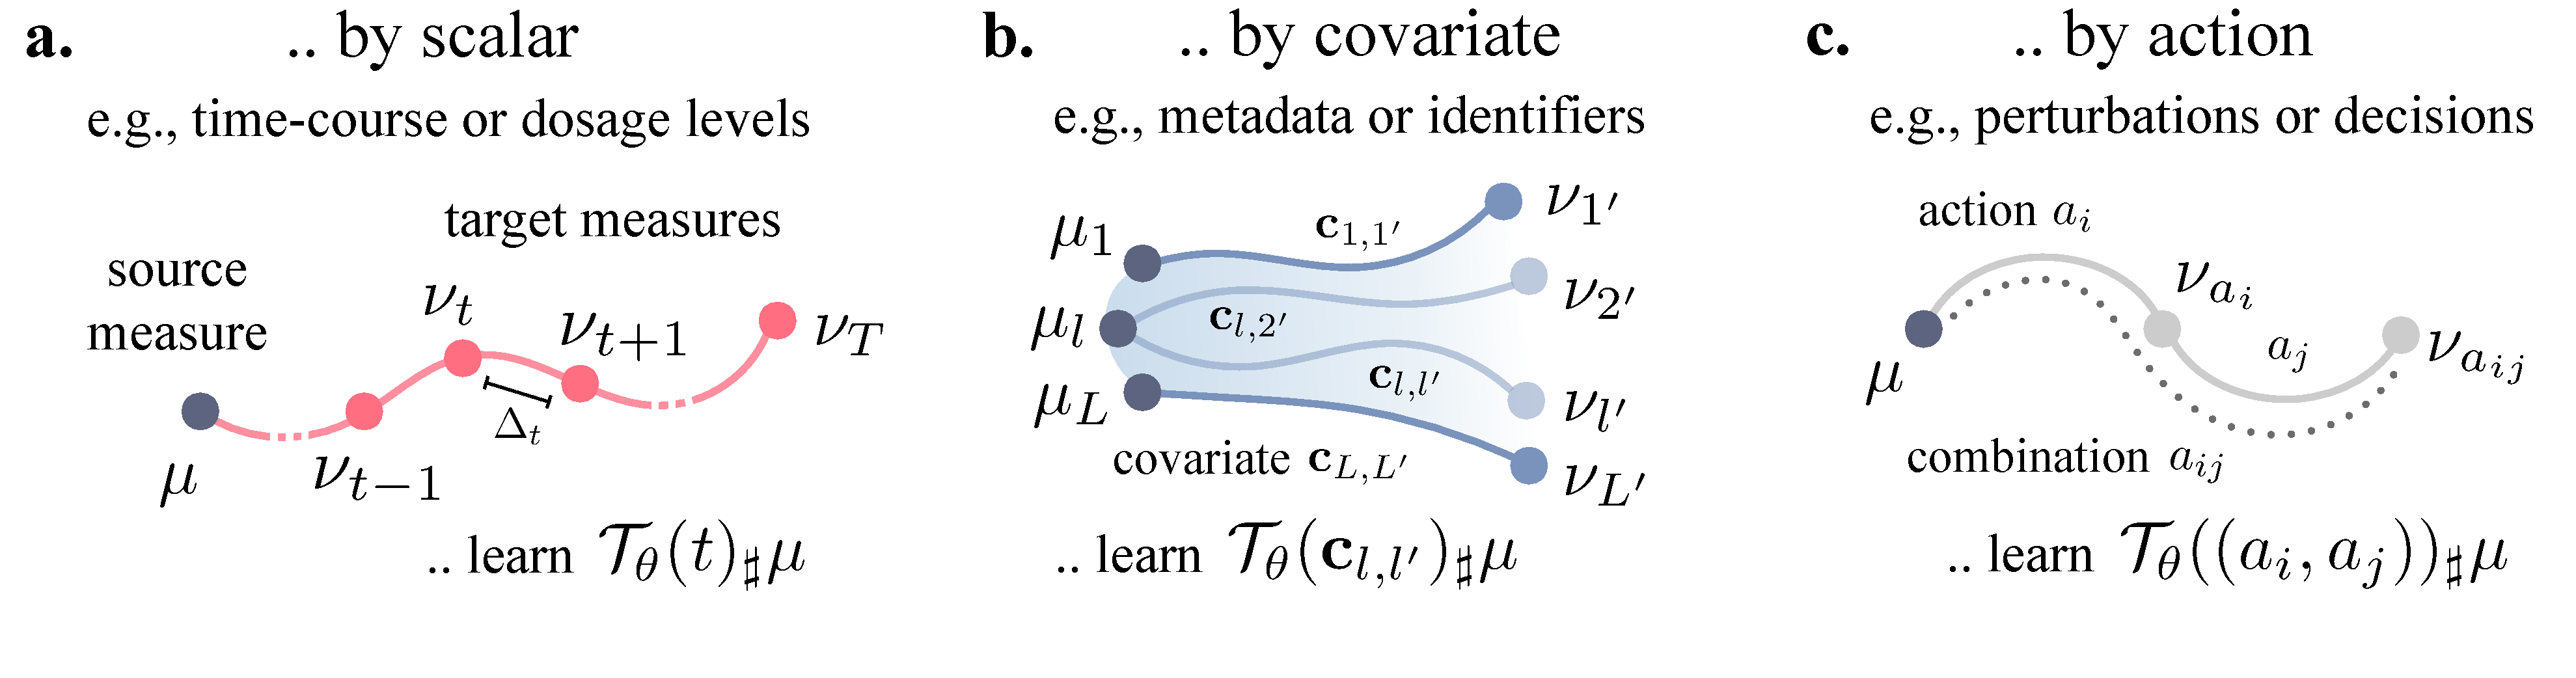
\includegraphics[width= \textwidth]{figures/fig_overview_condot.pdf}
    \caption{The evolution from a source $\mu$ to a target measure $\nu$ can depend on context variables $\cont$ of various nature. This comprises \textbf{a.} scalars such as time or dosage $t$ which determine the magnitude of the optimal transport, \textbf{b.} flow of measures into another one based on additional information (possibly different between $\mu$ and $\nu$) stored in vectors $\mathbf{c}_{l,l^\prime}$, or \textbf{c.} discrete and complex actions $a_i$, possibly in combination $a_{ij}$. We seek a unified framework to produce a map $\mathcal{T}_\theta(\cont)$ from any type of condition $\cont$. \vspace{-15pt}}
    \label{fig:overview_condot}
\end{figure*}


\section{\textsc{CondOT}: Supervised Training of Conditional Monge Maps} \label{sec:method}
We are given a dataset of $N$ pairs of measures, each endowed with a label, $(c_i,(\mu_i, \nu_i))\in\mathcal{C}\times \mathcal{P}(\RR^d)^2$. Our framework builds upon two pillars: (i.) we formulate the hypothesis that an optimal transport $T^\star_i$ (or, equivalently, the gradient of a convex potential $f^\star_i$) explains how measure $\mu_i$ was mapped to $\nu_i$, given context $c_i$; (ii.) we build on the multi-task hypothesis \citep{caruana1997multitask} that all of the $N$ maps $T^\star_i$ between $\mu_i$ and $\nu_i$ share a common set of parameters, that are \textit{modulated} by context information $c_i$. These ideas are summarized in an abstract regression model described below.

\subsection{A Regression Formulation for Conditional OT Estimation}
\looseness -1 $\theta\in\Theta\subset\mathbb{R}^r$, $\mathcal{T}_\theta$ describes a function that takes an input vector $c\in\mathcal{C}$, and outputs a \textit{function} $\mathcal{T}_\theta(c):\mathbb{R}^d\rightarrow\mathbb{R}^d$, as a hypernetwork would~\citep{ha2016hypernetworks}. Assume momentarily that we are given \textit{ground truth} maps $T_i$, that describe the effect of context $c_i$ on any measure, rather only pairs of measures $(\mu_i,\nu_i)$. This is of course a major leap of faith since even recovering an OT map $T^\star$ from two measures is in itself very challenging~\citep{hutter2021minimax,rigollet2022sample,pooladian2021entropic}. If such maps were available, a direct supervised approach to learn a unique $\theta$ could hypothetically involve minimizing a fit function composed of losses between maps
\begin{align}\label{eq:newobj1}
%\textstyle 
\min_\theta \sum_{i=1}^N \int_{\mathbb{R}^d} \|\mathcal{T}_{\theta}(c_i)(x) - T_i(x)\|^2\, \mathrm{d}\mu_i(x)\,.
\end{align}
Unfortunately, such maps $T_i$ are not given, since we are only provided unpaired samples before $\mu_i$ and after $\nu_i$ that map's application.
By \citeauthor{brenier1987decomposition}'s theorem, we know, however, that such an OT map $T^\star_i$ exists, and that it would be necessarily the gradient of a convex potential function that maximizes \eqref{eq:dual-cvx}. As a result, we propose to modify \eqref{eq:newobj1} to (i.) parameterize, for any $c$, the map $\mathcal{T}_\theta(c)$ as the gradient w.r.t. $x$ of a function $f_\theta(x,c):\mathbb{R}^d\times \mathcal{C}\rightarrow \mathbb{R}$ that is convex w.r.t. $x$, namely $\mathcal{T}_\theta(\cont) := x \mapsto \nabla_1 f_\theta(x,\cont)$; (ii.) estimate $\theta$ by maximizing \textit{jointly} the dual objectives~\eqref{eq:dual-cvx} simultaneously for all $N$ pairs of measures, in order to ensure that the maps are close to optimal, to form the aggregate problem
\begin{align}\label{eq:supdual} 
\textstyle \max_\theta \sum_{i=1}^N \mathcal{E}_{\mu_i,\nu_i}(f_{\theta}(\,\cdot\,, c_i)).
\end{align}
We detail in \cref{sec:neural_solvers} how the Legendre transforms that appear in the energy terms $\mathcal{E}_{\mu_i,\nu_i}$ are handled with an auxiliary function.

\subsection{Integrating Context in Convex Architectures}
We propose to incorporate context variables, in order to modulate a family of convex functions $f_{\theta}(x, c)$
using \acrlongpl{PICNN}. \acrshortpl{PICNN} are neural networks that can be evaluated over a pair of inputs $(x,\cont)$, but which are only required to be convex w.r.t.~$x$. Given an input vector $x$ and context vector $\cont$, a ${L}$-layer PICNN is defined as $\varphi_\theta(x, c) = z_{L},$ where, recursively for $0 \leq {l} \leq {L}-1$ one has
\begin{equation} \label{eq:picnn}
\begin{aligned} 
u_{{l}+1} =&\, a^\prime_{l}\left(V_{l} u_{l}+v_{l}\right), \\
z_{{l}+1} =&\, a_{l}\left(W_{l}^{z}\left(z_{l} \circ\left[W_{l}^{z u} u_{l}+b_{l}^{z}\right]_+\right)+\right.
\left.W_{l}^{x}\left(x \circ(W_{l}^{x u} u_{l}+b_{l}^{x})\right)+W_{l}^{u} u_{l}+b_{l}^u\right), \\
\end{aligned}
\end{equation}
where the PICNN is initialized as $u_{0}=\cont, z_0 = \mathbf{0}$, $\circ$ denotes the Hadamard element-wise product, and $a^\prime_{l}$ is any activation function. The parameters of the PICNN are then given by
$$\theta = \{ V_{l}, W_{l}^{z}, W_{l}^{z u}, W_{l}^{x}, W_{l}^{x u} , W_{l}^{u}, v_{l}, b_{l}^{z}, b_{l}^{x}, b_{l}^u \}.$$ 
Similar to ICNNs, the convexity w.r.t. input variable $x$ is guaranteed as long as activation functions $a_i$ are convex and non-decreasing, and the weight matrices $W_{l}^{z}$ have non-negative entries. We parameterize this by storing them as element-wise applications of softplus operations on precursor matrices of the same size, or, alternatively, by regularizing their negative part. Finally, much like ICNNs, all matrices at the ${L}-1$ layer are line vectors, and their biases scalars.

Such networks were proposed by \citet[Eq. 3]{amos2017input} to address a problem that is somewhat symmetric to ours: Their inputs were labeled as $(y, x)$, where $y$ is a label vector, typically much smaller than that of vector $x$. Their PICNN is convex w.r.t.~$y$, in order to easily recover, given a datapoint $x$ (e.g., an image) the best label $y$ that corresponds to $x$ using gradient descent as a subroutine, i.e. $y^\star(x) = \arg\min_y \text{PICNN}_\theta(x,y)$. PICNNs were therefore originally proposed to learn a parameterized, implicit classification layer, amortized over samples, whose motivation rests on the property that it is convex w.r.t. label variable $y$. By contrast, we use PICNNs that are convex w.r.t. data points $x$. In addition to that swap, we do not use the convexity of the PICNN to define an implicit layer (or to carry out gradient descent). Indeed, it does not make sense in our setting to minimize $\varphi_\theta(x,\cont)$ as a function of $x$, since $x$ is an observation. Instead, our proposal rests on the property that $\nabla_1 \varphi_\theta(x,\cont)$ describes a parameterized family of OT maps. We note that PICNNs were considered within the context of OT in \cite[Appendix B]{fan2021scalable}. In that work, PICNNs provide an elegant reformulation for neural Wasserstein barycenters. \citet{fan2021scalable} considered a context vector $c$ that was restricted to be a small vector of probabilities.


\subsection{Conditional Monge Map Architecture}\label{subsec:combin}
Using PICNNs as a base module, the \textsc{CondOT} architecture integrates operations on the contexts $\gC$. As seen in Figure~\ref{fig:overview_condot}, context values $\cont$ may take various forms:
\begin{enumerate}[noitemsep,leftmargin=.35cm,topsep=0pt,parsep=0pt,partopsep=0pt]
\item A scalar $t$ denotes a strength or a temporal effect. For instance, \citeauthor{mccann1997convexity}'s interpolation \eqref{eq:mccann_interpolation} and its time parameterization, $\alpha_{t}=((1-t) \operatorname{Id}+t T)_{\sharp} \alpha_{0}$ \citep{mccann1997convexity} can be interpreted as a trivial conditional OT model that creates, from an OT map $\varphi_\theta$, a set of maps parameterized by $t$, $\mathcal{T}_\theta(t):=x\mapsto\nabla_x \left((1-t)\|x\|^2/2 +t \varphi_\theta(x)\right)$.
% \textsc{CondOT} can describe consecutive optimal displacements $\alpha_t$ from $t=0$ to any time $t$, but which are not  Wasserstein geodesic.
\item A covariate vector influencing the nature of the effect that led $\mu_i$ to $\nu_i$, (capturing, e.g., patient feature vectors).
\item One or multiple actions, possibly discrete, representing decisions or perturbations applied onto $\mu_i$. \\
\end{enumerate}

To provide a flexible architecture capable of modeling different types of conditions as well as conditions appearing in combinations, the more general \textsc{CondOT} architecture consists of the hypernetwork $\mathcal{T}_\theta$ that is fed a context vector through embedding and combinator modules. This generic architecture provides a one-size fits all approach to integrate all types of contexts $\cont$.

\subsubsection{Embedding Module $\mathcal{E}$}
\looseness -1 To give greater flexibility when setting the context variable $c$, \textsc{CondOT} contains an embedding module $\mathcal{E}$ that translates arbitrary contexts into real-valued vectors. Besides simple scalars $t$ (\cref{fig:overview_condot}a) for which no embedding is required, discrete contexts can be handled with an embedding module $\mathcal{E}_\phi$.

\paragraph{One-hot encoding $\mathcal{E}_\text{ohe}$.}
When the set $\gC$ is small, this can be done effectively using a \acrfull{OHE} $\mathcal{E}_\text{ohe}$.
Thus, covariates, such as subpopulations or patient identifiers, can be simply embedded via one-hot encodings. These embeddings, however, are not able to capture unknown covariates after training.

For more complicated actions $a$ such as treatments, there is no simple way to vectorize a context $c$. Similarly to action embeddings in reinforcement learning \citep{chandak2019learning, tennenholtz2019natural}, we can learn embeddings for discrete actions into a learned continuous representation.
This often requires domain knowledge of the context values. For molecular drugs, for example, we can learn molecular representations $\mathcal{E}_\text{mol}$ such as chemical, motif-based~\citep{rogers2010extended} or neural fingerprints~\citep{rong2020grover, schwaller2022machine, rogers2010extended}.
However, often this domain knowledge is not available. 
% In the case of genetic perturbations, for example, no straightforward embedding is available.
% We might, however, have some sparse sample-access to an action $a$'s target effects (i.e., when modeling the effect of actions in combination, we often have sample access to an action applied in isolation).

\begin{wrapfigure}{r}{0.4\textwidth}
    \centering
    %\vskip-0.1cm
    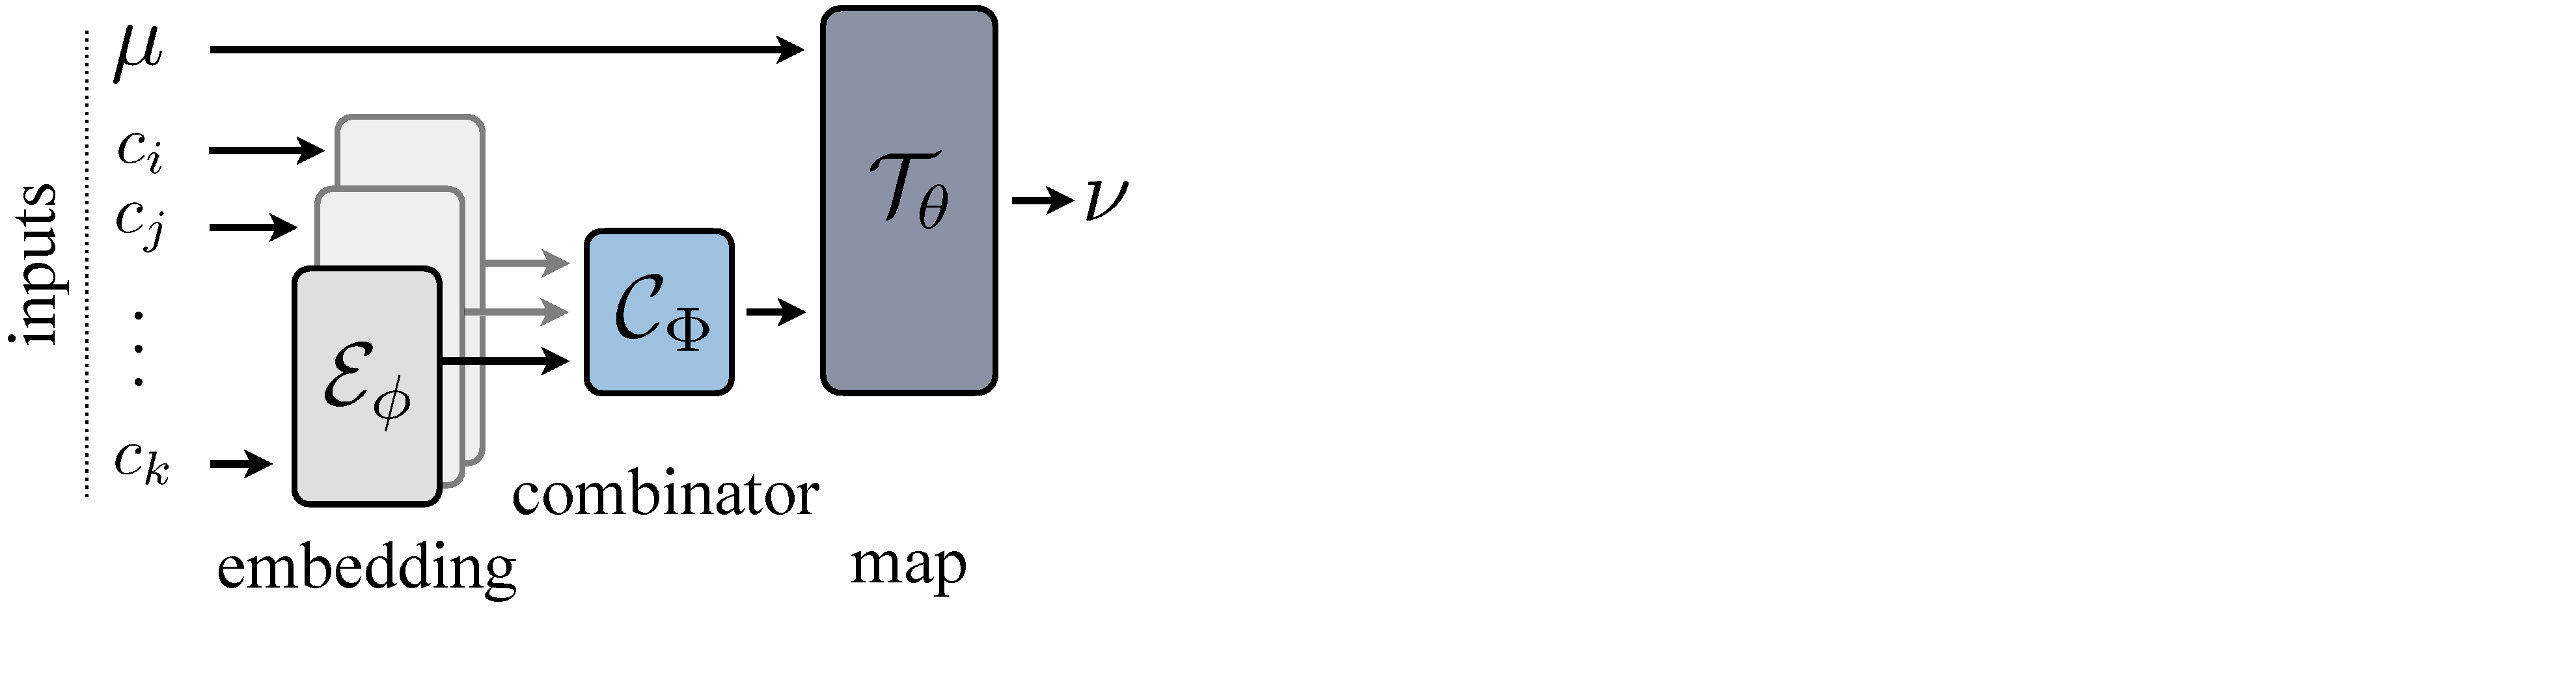
\includegraphics[width=0.4\textwidth]{figures/fig_architecture.pdf}
    \caption{\textbf{\textsc{CondOT} Architecture and Modules}. The embedding module $\mathcal{E}_\phi$ embeds arbitrary conditions $c$, which are then combined via module $\mathcal{C}_\Phi$. Using the processed contexts $c$, the map $\mathcal{T}_\theta(c)$ acts on $\mu$ to predict the target measure $\nu$. \vspace{-10pt}}
    \label{fig:architecture}
\end{wrapfigure}

\paragraph{Mode of action embedding $\mathcal{E}_\text{moa}$.}
In \textsc{CondOT}, we thus construct so-called \acrfull{MOA} embeddings, by computing an embedding $\mathcal{E}_\text{moa}$ that encourages actions $a$ with a similar effect on target population $\nu$ to have a similar representation.
Such mode-of-action embeddings map actions into a latent space based on their mechanism of action and effect on the target population.
In the fashion of word embeddings \citep{mikolov2013efficient, mikolov2013distributed, mikolov2013linguistic}, we require actions with similar effects to be closely embedded in the learned representation.
This means, however, that we require some sample access of target population particles, i.e., perturbed cells by individual compounds (not in combination).
While several metric embeddings are possible \citep{chopra2005learning}, we here test a simple multi-dimensional scaling-based embedding \citep{mead1992review}.
For this, we compute the pairwise Wasserstein distance matrix between all target populations of different individual perturbations. We then compute a 10-dimensional MDS embedding based on the stress minimization using a majorization algorithm (\texttt{smacof}) \citep{de2009multidimensional} of \texttt{sklearn} \citep{pedregosa2011scikit}, which serves as a descriptor for each individual perturbation.
In \cref{sec:evaluation_condot}, we analyze several embedding types for different use cases.

\subsubsection{Combinator Module $\mathcal{C}$}
\looseness -1 While we often have access to contexts $c$ in isolation, it is crucial to infer the effect of contexts applied in combination. A prominent example is cancer combination therapies, in which multiple treatment modalities are administered in combination to enhance treatment efficacy \citep{kummar2010utilizing}.
In these settings, the mode of operation between individual contexts $c$ is often not known, and can thus not be directly modeled via simple arithmetic operations such as 
\texttt{min, max, sum, mean}.
While we test as a baseline the case, applicable to one-hot-embeddings, where simple additions are used to model these combinations, we propose to augment the \textsc{CondOT} architecture with a parameterized combinator module $\mathcal{C}_\Phi$. We consider the following combinator modules:

\paragraph{Multi-hot combinator $\mathcal{C}^\text{ohe}_+$.}
A na\"ive way of constructing the combinator is to combine different actions via multi-hot encodings. If all single perturbations are observed during training, each individual action can be represented via a one-hot encoding. The potential combination of different actions is then encoded by adding the respective one-hot encodings, resulting in a multi-hot encoding for each combination.
A limitation of this embedding, however, is that it cannot generalize to unknown actions after training.

\paragraph{Deep set combinator $\mathcal{C}^\text{moa}_\Phi$.}
When not considering one-hot-based embeddings and when aiming to generalize to unseen perturbations, we need a combinator module that learns how to associate different individual embeddings with each other to receive a joint embedding.
As we, for now, do not make an assumption on the order of the perturbation, we consider a permutation-invariance network architecture such as deep sets \citep{zaheer2017deep} with parameters $\Phi$. Taking a set of arbitrary size $k$ containing individual context embeddings $\{\mathcal{E}_\text{moa}(c^1), \mathcal{E}_\text{moa}(c^2), \dots, \mathcal{E}_\text{moa}(c^k)\}$, it returns a learned combination embedding $\hat{c}_i = \mathcal{C}_\Phi(\mathcal{E}_\text{moa}(c^1), \mathcal{E}_\text{moa}(c^2), \dots, \mathcal{E}_\text{moa}(c^k))$.
% If interactions between the context variables exist, $\mathcal{C}_\Phi$ can be represented via classical message-passing network architectures~\citep{gilmer2020message,kipf2018neural}.
Receiving a flexible number of inputs from the embedding module $\mathcal{E}_\phi$, \textsc{CondOT} allows for joint training of the PICNN parameters $\theta$, embedding parameters $\phi$, and combinator parameters $\Phi$ in a single, end-to-end differentiable architecture.


\subsubsection{Training Procedure}

\looseness -1 Given a dataset $\mathcal{D}=\{c_i, (\mu_i, \nu_i) \}_{i=0}^N$ of $N$ pairs of populations before $\mu_i$ and after transport $\nu_i$ connected to a context $c_i$, we follow a similar strategy as introduced in \cref{sec:neural_solvers} to learn map $\mathcal{T}_\theta(c_i)$. 
The training loss aims at making sure the map $\mathcal{T}_\theta(c_i)$ is an OT map from $\mu_i$ to $\nu_i$, where $c_i$ may either be the original label itself or its embedded/combined formulation in more advanced tasks. To handle the Legendre transform in \eqref{eq:dual-cvx}, we use the proxy dual objective defined in \eqref{eq:ot-minmax} \citep{makkuva2020optimal} in place of \eqref{eq:dual-cvx} to minimize our overall loss~\eqref{eq:supdual}.

We then parameterize the potentials $\varphi$ and $g$ using two PICNNs, i.e., $\text{PICNN}_{\theta}$ and $\text{PICNN}_{\phi}$, that already integrate an embedding and/or combinator module. The regularization in \eqref{eq:ot-minmax} thereby promotes that for any $c$, $\text{PICNN}_{\phi}(\cdot,c)$ resembles the Legendre transform of the other network, i.e., $\text{PICNN}_{\theta^\star}(\cdot,c)$.
Parameters of all three modules are trained jointly through the alternate min-max optimization introduced in \eqref{eq:cellot-optim}, replacing the \acrshort{ICNN} architecture in loss functions \eqref{eq:makkuva_f_loss}-\eqref{eq:makkuva_g_loss} with \acrshortpl{PICNN}, i.e.,
\begin{align*} 
    \ell_\varphi(\mu, \nu, c; \theta) &= \mathbb{E}_{x \sim \mu}[\text{PICNN}_{\phi}(x, c)] - \mathbb{E}_{y \sim \nu}[\text{PICNN}_{\theta}(\nabla \text{PICNN}_{\phi}(y, c), c)], \\
    \ell_g(\mu, \nu, c; \phi) &= -\mathbb{E}_{y \sim \nu}[\langle y, \nabla \text{PICNN}_{\phi}(y, c)\rangle-\text{PICNN}_{\theta}(\nabla \text{PICNN}_{\phi}(y, c), c)].
\end{align*}
For more details, see \cref{sec:neural_solvers}.

\begin{table*}[t]
    \caption{Evaluation of drug effect predictions from control cells to cells treated with drug Givinostat when conditioning on various covariates influencing cellular responses such as drug dosage and cell type. Results are reported based on MMD and the $\ell_2$ distance between perturbation signatures of marker genes in the 1000-dimensional gene expression space.}
    \label{tab:exp_scalar_covariate_sciplex}
    \centering
\adjustbox{max width=\linewidth}{%
    \begin{tabular}{lccccc}
    \toprule
         \textbf{Method} & \multicolumn{5}{c}{\textbf{Conditioned on Drug Dosage}} \\
         & \multicolumn{2}{c}{In-Sample} && \multicolumn{2}{c}{Out-of-Sample}\\
         \cmidrule{2-3} \cmidrule{5-6}
         & MMD & $\ell_2(\text{PS})$ && MMD & $\ell_2(\text{PS})$ \\
    \midrule
        \textsc{CPA} \citep{lotfollahi2021compositional} & 0.1502 $\pm$ 0.0769 & 2.47 $\pm$ 2.89 && 0.1568 $\pm$ 0.0729 & 2.65 $\pm$ 2.75 \\
        \textsc{ICNN OT} \citep{makkuva2020optimal} & 0.0365 $\pm$ 0.0473 & 2.37 $\pm$ 2.15 && 0.0466 $\pm$ 0.0479 & 2.24 $\pm$ 2.39 \\
        \textsc{CondOT} (Identity initialization) & 0.0111 $\pm$ 0.0055 & 0.63 $\pm$ 0.09 && 0.0374 $\pm$ 0.0052 & 2.02 $\pm$ 0.10 \\
        \textsc{CondOT} (Gaussian initialization) & 0.0128 $\pm$ 0.0081 & 0.60 $\pm$ 0.11 && 0.0325 $\pm$ 0.0062 & 1.84 $\pm$ 0.14 \\
    \bottomrule  \\
    \end{tabular}
}
	\raggedright
\adjustbox{max width=.66\linewidth}{%
	\begin{tabular}{lcccccccc}
    \toprule
         \textbf{Method} & \multicolumn{2}{c}{\textbf{Conditioned on Cell Line}} \\
         & \multicolumn{2}{c}{In-Sample} \\
         \cmidrule{2-3}
         & MMD & $\ell_2(\text{PS})$ \\
    \midrule
        \textsc{CPA} \citep{lotfollahi2021compositional} & 0.2551 $\pm$ 0.006 & 2.71 $\pm$ 1.51 \\
        \textsc{ICNN OT} \citep{makkuva2020optimal} & 0.0206 $\pm$ 0.0109 & 1.16 $\pm$ 0.75 \\
        \textsc{CondOT} (Identity initialization) & 0.0148 $\pm$ 0.0078 & 0.39 $\pm$ 0.06 \\
        \textsc{CondOT} (Gaussian initialization) & 0.0146 $\pm$ 0.0074 & 0.41 $\pm$ 0.07 \\
    \bottomrule
    \end{tabular}
}
\end{table*}

\begin{figure*}
    \centering
    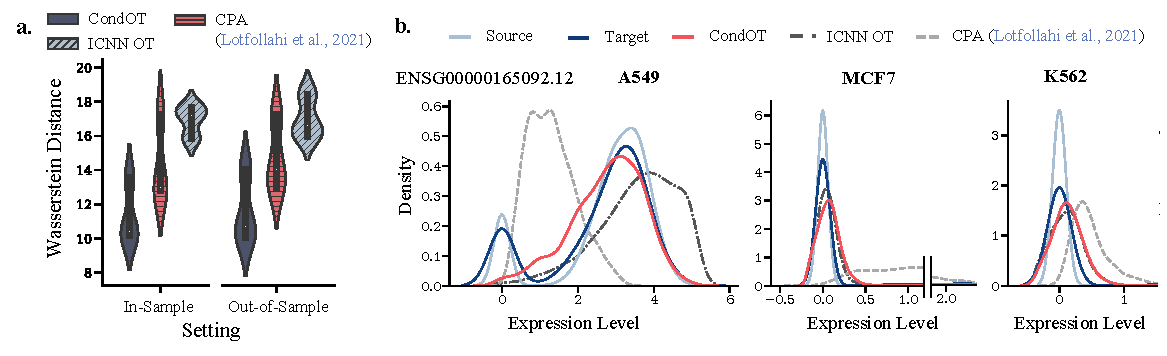
\includegraphics[width=\textwidth]{figures/fig_sciplex_main_results.pdf}
    \caption{\textbf{a.} \looseness -1 Predictive performance of \textsc{CondOT} and baselines w.r.t. the entropy-regularized Wasserstein distance on drug dosages \emph{in-sample}, i.e., seen during training, and \emph{out-of-sample}, i.e., unseen during training. \textbf{b.} Marginal distributions of observed source and target distributions, as well as predictions on perturbed distributions by \textsc{CondOT} and baselines of an exemplary gene across different cell lines. The predicted marginals of each method should match the marginal of the target population.}
    \label{fig:exp_scalar_sciplex}
\end{figure*}

\section{Empirical Evaluation} \label{sec:evaluation_condot}

\looseness -1 Biological cells undergo changes in their molecular profiles upon chemical, genetic, or mechanical perturbations. These changes can be measured using recent technological advancements in high-resolution multivariate single-cell biology. Measuring single cells in their unperturbed or perturbed state requires, however, destroying them, resulting in populations $\mu$ and $\nu$ that are unpaired. The relevance of OT to that comes from its ability to resolve such ambiguities through OT maps, 
% which can provide more general functions that can predict molecular responses, 
holding promises of a better understanding of health and disease. 
We consider various high-dimensional problems arising from this scenario to evaluate the performance of \textsc{CondOT} versus other baselines.
% Here we assume that  capture that cells at any time are drawn from a probability distribution in gene-expression space.

\subsection{Modeling Dosage-Sensitive Treatment Responses to Cancer Drugs} \label{sec:eval_scalar}

% The evolution of single-cell populations during a developmental process can be monitored by sampling, every now and then, representative cells of the system, and measuring their gene expression features in order to trace the differentiation across multiple snapshots.
% Inferring a matching of ancestor to descendant fates is a crucial step toward a better understanding of the molecular programs that guide cell differentiation of these evolutionary processes.

% In the following, we apply \textsc{CondOT} to embryoid body single-cell RNA sequencing (scRNA-seq) data \citep{moon2019}, describing the differentiation of human embryonic stem cells grown as embryoid bodies into diverse cell lineages over a period of 27 days.
% We aim at infering the transport map $T_\theta(\delta t)$ which predicts the development of a cell population at time $t_i$ into cell states at time $t_{i+1}$, i.e., $T_\theta(\delta t)_\sharp \mu_{i} = \mu_{i+1}$, where $\delta t = t_{i+1} - t_{i}$.
% We learn $T_\theta$ by utilizing \citeauthor{brenier1987decomposition}'s theorem and parameterizing $T_\theta = \nabla \text{PICNN}_\theta$ taking as input the measure at the previous time point $\mu_{i}$ as well as the time interval $\delta t$ during which the cells are expected to evolve (see \cref{sec:neural_primal} for more details).
% We compare our method to classical forward Euler schemes, previously proposed to learn time-varying single-cell dynamics \citep{hashimoto2016learning, bunne2022proximal}.

% Small molecular drugs can have profound effects on the cellular phenotype by altering signaling cascades and other molecular programs.
\looseness -1 Upon application of a molecular drug, the state of each cell $x_i$ of the unperturbed population is altered, and observed in population $\nu$.
Molecular drugs are often applied at different dosage levels $t$, and the magnitude of changes in the gene expression profiles of single cells highly correlates with that dosage. 
We seek to learn a global, parameterized transport map $\mathcal{T}_\theta$ sensitive to that dosage.% and accurately describe perturbed cellular states at different dosage levels.
We evaluate our method on the task of inferring single-cell perturbation responses to the cancer drug Givinostat, a histone deacetylase inhibitor with potential anti-inflammatory, anti-angiogenic, and antineoplastic activities \citep{srivatsan2020massively}, applied at different dosage levels, i.e., $t \in \{10\,$nM, $100\,$nM, $1,000\,$nM, $10,000\,$nM$\}$. The dataset contains $3,541$ cells described with the gene expression levels of $1,000$ highly-variable genes.
In a first experiment, we measure how well \textsc{CondOT} captures the drug effects at different dosage levels via distributional distances such as MMD~\citep{gretton2012kernel} and the $\ell_2$-norm between the corresponding \acrfull{PS}, as well as the entropy-regularized Wasserstein distance~\citep{cuturi2013sinkhorn}. We compute the metrics on 50 marker genes, i.e., genes mostly affected upon perturbation.
To put \textsc{CondOT}'s performance into perspective, we compare it to current state-of-the-art baselines~\citep{lotfollahi2021compositional} as well as parameterized Monge maps without context variables \citep[\textsc{ICNN OT}]{bunne2021learning, makkuva2020optimal}.
As visible in Table~\ref{tab:exp_scalar_covariate_sciplex} and \cref{fig:exp_scalar_sciplex}a, \textsc{CondOT} achieves consistently more accurate predictions of the target cell populations at different dosage levels than OT approaches that cannot utilize context information, demonstrated through a lower average loss and a smaller variance.
This becomes even more evident when moving to the setting where the population has been trained only on a subset of dosages and we test \textsc{CondOT} on \emph{out-of-sample} dosages. Table~\ref{tab:exp_scalar_covariate_sciplex} and \cref{fig:exp_scalar_sciplex}a demonstrate that \textsc{CondOT} is able to generalize to previously \emph{unknown} dosages, thus learning to interpolate the perturbation effects from dosages seen during training.
% We further provide an additional comparison of \textsc{CondOT}, operating in the multi-task setting, to the single-task performance of optimal transport-based methods \cref{app:add_baseline}. While the single-task setting of course fails to generalize to new contexts and requires all contexts to be distinctly known, it provides us with a \textit{pseudo} lower bound, which \textsc{CondOT} is able to reach (see Table~\ref{tab:lower_bound}).
% For dosages, we build a dosage encoder module $\mathcal{E}_\text{dosage}$ which can integrate known dosage-response curves (e.g., linear, sigmoid, or more complex relationships). ...

\begin{figure*}[t]
    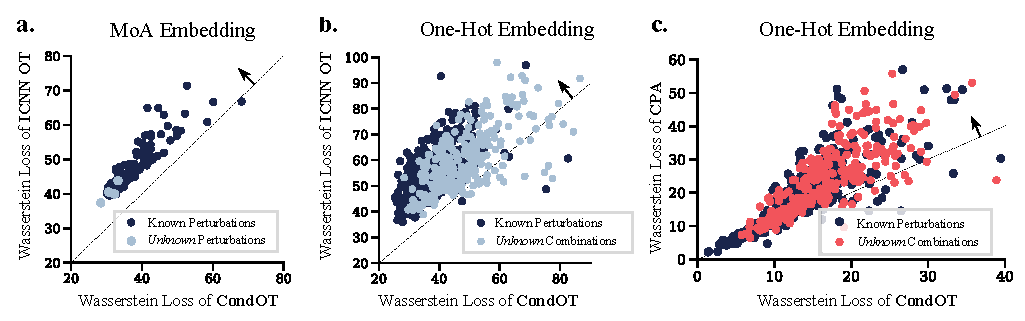
\includegraphics[width=\textwidth]{figures/fig_action_comb_comparison_scatter.pdf}
    \caption{Comparison between \textbf{a.} \textsc{CondOT} and \textsc{ICNN OT}~\citep{makkuva2020optimal} based on embedding $\mathcal{E}_\text{moa}$ \textbf{b.} as well as $\mathcal{E}_\text{ohe}$, and \textbf{c.} \textsc{CondOT} and \textsc{CPA}~\citep{lotfollahi2021compositional} based on embedding $\mathcal{E}_\text{ohe}$ on \emph{known} and \emph{unknown} perturbations or combinations. Results above the diagonal suggest the higher predictive performance of \textsc{CondOT}.}
    \label{fig:exp_action_norman_scatter}
\end{figure*}


\subsection{Predicting Cell Type-Specific Treatment Responses to Cancer Drugs} \label{sec:eval_covariate}

\looseness -1 Molecular processes are often highly dependent on additional covariates that steer experimental conditions, and which are not present in the features measures in population $\mu$ or $\nu$.
This can be, for instance, factors such as different cell types clustered within the populations.
When the model can only be conditioned w.r.t. a small and \textit{fixed} set of metadata information, such as cell types, it is sufficient to encode these contexts using a one-hot encoding module $\mathcal{E}_\text{ohe}$.
To illustrate this problem, we consider cell populations comprising three different cell lines (A549, MCF7, and K562). As visible in Table~\ref{tab:exp_scalar_covariate_sciplex}, \textsc{CondOT} outperforms current baselines which equally condition on covariate information such as \textsc{CPA}~\citep{lotfollahi2021compositional}, assessed through various evaluation metrics.
Figure~\ref{fig:exp_scalar_sciplex}b displays a gene showing highly various responses towards the drug Givinostat dependent on the cell line. \textsc{CondOT} captures the distribution shift from control to target populations consistently across different cell lines.

\subsection{Inferring Genetic Perturbation Responses}

\looseness -1 To recommend personalized medical procedures for patients, or to improve our understanding of genetic circuits, it is key to be able to predict the outcomes of novel perturbations, arising from combinations of drugs or genetic perturbations. 
Rather than learning individual maps $T_\theta^a$ predicting the effect of individual treatments, we aim at learning a global map  $\mathcal{T}_\theta$ which, given as input the unperturbed population $\mu$ as well as the action $a$ of interest, predicts the cell state perturbed by $a$.
Thanks to its modularity, \textsc{CondOT} can not only learn a map $T_\theta$ for all actions \emph{known} during training but also generalize to \emph{unknown} actions, as well as potential \emph{combinations} of actions. We will discuss all three scenarios below.

\subsubsection{\textit{Known} Actions}
\label{sec:eval_action_known}

\looseness -1 In the following, we analyze \textsc{CondOT}'s ability to accurately predict phenotypes of genetic perturbations based on single-cell RNA-sequencing pooled \acrfull{CRISPR} screens \citep{norman2019exploring, dixit2016perturb}, comprising $98,419$ single-cell gene expression profiles with $92$ different genetic perturbations, each cell measured via a $1,500$ highly-variable gene expression vector.
As, in the first step, we do not aim at generalizing beyond perturbations encountered during training, we utilize again a one-hot encoding $\mathcal{E}_\text{ohe}$ to condition $\mathcal{T}_\theta$ on each perturbation $a$.
We compare our method to other baselines capable of modeling effects of a large set of perturbations such as \textsc{CPA} \citep{lotfollahi2021compositional}.
Often, the effect of genetic perturbations is subtle in the high-dimensional gene expression profile of single cells. Using ICNN-parameterized OT maps without context information, we can thus assess the gain in accuracy of predicting the perturbed target population by incorporating context awareness over simply predicting an average perturbation effect. 
Figure~\ref{fig:exp_action_norman_scatter}a and b demonstrate that compared to OT ablation studies, \cref{fig:exp_action_norman_scatter}c and \cref{fig:exp_action_norman_line}a for the current state-of-the-art method \textsc{CPA}~\citep{lotfollahi2021compositional}. Compared to both, \textsc{CondOT} captures the perturbation responses more accurately w.r.t. the Wasserstein distance.

\begin{figure*}[t]
    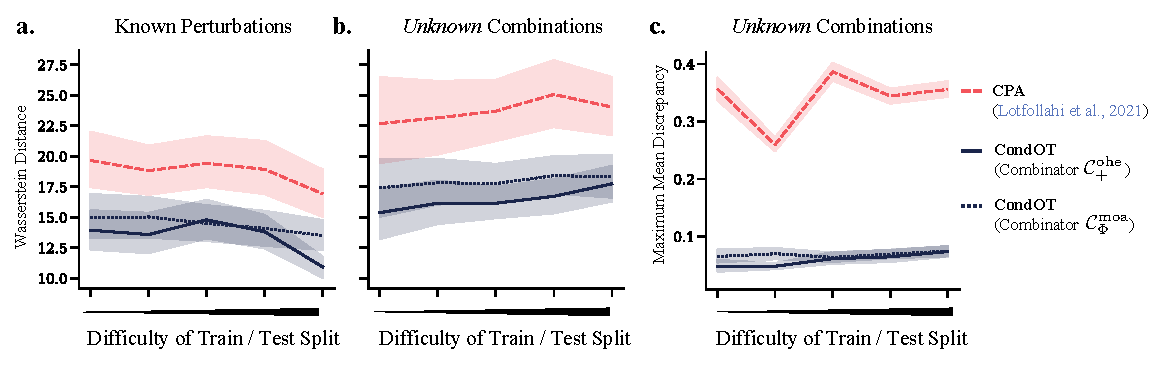
\includegraphics[width=1.1\textwidth]{figures/fig_action_comb_comparison_metrics.pdf}
    \caption{Predictive performance for \textbf{a.} known perturbations, \textbf{b.} unknown perturbations in combination w.r.t. regularized Wasserstein distance and \textbf{c.} MMD over different train/test splits of increasing difficulty for baseline \textsc{CPA} as well as \textsc{CondOT} with different combinators $\mathcal{C}^\text{ohe}_+$ and $\mathcal{C}^\text{moa}_\Phi$.}
    \label{fig:exp_action_norman_line}
\end{figure*}


\subsubsection{\textit{Unknown} Actions}
\label{sec:eval_action_unknown}

\looseness -1 With the emergence of new perturbations or drugs, we aim at inferring cellular responses to settings not explored during training.
One-hot encodings, however, do not allow us to model \emph{unknown} perturbations. 
This requires us to use an embedding $\mathcal{E}$, which can provide us with a representation of an unknown action $a^\prime$.
As genetic perturbations further have no meaningful embeddings as, for example, molecular fingerprints for drugs, we resort to mode-of-action embeddings introduced in \cref{subsec:combin}. Assuming marginal sample access to all individual perturbations, we compute a \acrfull{MDS}-based embedding from pairwise Wasserstein distances between individual target populations, such that perturbations with similar effects are closely represented. 
As current state-of-the-art methods are restricted to modeling perturbations via one-hot encodings, we compare our method to \textsc{ICNN OT} only. As displayed in \cref{fig:exp_action_norman_scatter}a, \textsc{CondOT} accurately captures the response of \emph{unknown} actions (BAK1, FOXF1, MAP2K6, MAP4K3), which were not seen during training, at a similar Wasserstein loss as perturbation effects seen during training.
 
 \begin{figure*}
    \centering
    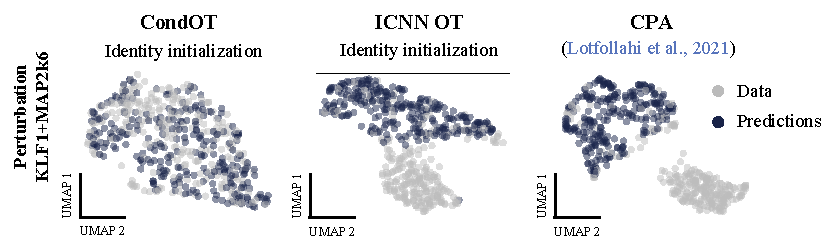
\includegraphics[width=0.9\textwidth]{figures/fig_action_comb_comparison_umap.pdf}
    \caption{\looseness -1 \acrshort{UMAP} embeddings of cells perturbed by the combination KLF1+MAP2K6 (gray) and predictions of \textsc{CondOT} (ours), \textsc{ICNN OT}~\citep{makkuva2020optimal}, and \textsc{CPA} (blue). While \textsc{CondOT} aligns well with observed perturbed cells, the baselines fail to capture subpopulations.}
    \label{fig:action_comb_comparison_umap}
\end{figure*}
 

\subsubsection{Actions in Combination}
\label{sec:eval_action_comb}

\looseness -1 While experimental studies can often measure perturbation effects in biological systems in isolation, the combinatorial space of perturbations in composition is too large to capture experimentally. Often, however, combination therapies are cornerstones of cancer therapy \citep{mokhtari2017combination}.
In the following, we test different combinator architectures to predict genetic perturbations in combination with single targets.
Similarly to \citet{lotfollahi2021compositional}, we can embed combinations by adding individual one-hot encodings of single perturbations (i.e., $\mathcal{C}^\text{ohe}_+$). In addition, we parameterize a combinator via a permutation-invariant deep set, as introduced in \cref{subsec:combin}, based on mode-of-action embeddings of individual perturbations (i.e., $\mathcal{C}^\text{moa}_\Phi$). 
We split the dataset into train/test splits of increasing difficulty: Initially containing all individual perturbations as well as some combinations, the number of perturbations seen in combination during training decreases over each split.
We compare different combinators to \textsc{ICNN OT} (\cref{fig:exp_action_norman_scatter}b) and \textsc{CPA}~\citep{lotfollahi2021compositional} (\cref{fig:exp_action_norman_scatter}c, \cref{fig:exp_action_norman_line}b, c). While the performance drops compared to inference on \emph{known} perturbations (\cref{fig:exp_action_norman_line}a) and decreases with increasing difficulty of the train/test split, \textsc{CondOT} outperforms all baselines.
When embedding these high-dimensional populations in a low-dimensional \acrshort{UMAP} space~\citep{umap}, one can see that \textsc{CondOT} captures the entire perturbed population, while \textsc{ICNN OT} and \textsc{CPA} fail in capturing certain subpopulations in the perturbed state (see \cref{fig:action_comb_comparison_umap}).


\section{Discussion}
We have developed the \textsc{CondOT} framework that is able to infer OT maps from not only one pair of measures but many pairs that come labeled with a context value. To ensure that \textsc{CondOT} encodes optimal transports, we parameterize it as a PICNN, an input-convex NN that modulates the values of its weights matrices according to a sequence of feature representations of that context vector. We showcased the generalization abilities of \textsc{CondOT} in the extremely challenging task of predicting outcomes for unseen combinations of treatments. These abilities and PICNN more generally hold several promises, both as an augmentation of the \texttt{OTT} toolbox~\citep{cuturi2022optimal} and for future applications of OT to single-cell genomics.


\part{Dynamic Neural Optimal Transport} \label{part:dynamic_not}
\cleardoublepage%
\chapter[Learning Dynamical Systems via OT and Gradient Flows]{Learning Dynamical Systems via Optimal Transport and Gradient Flows}
\label{cha:neural_pde}

\dictum[Andrey Kolmogorov, \textit{\"Uber die analytischen Methoden in der Wahrscheinlichkeitsrechnung} (1931)]{%
  Ein solches mathematisch-definierbares System ist \"uberhaupt nicht die Wirklichkeit selbst, sondern nur ein Schema, welches zur Beschreibung der Wirklichkeit dienen kann.} % This mathematically defined system is not a reality itself, but a scheme that can be used to describe reality. From: On Analytical Methods in the Theory of Probability
\vskip 1em

\verpar{Contributions}{
Most of the material in this chapter has been already published in the following conference proceedings:
\begin{itemize}
	\item[] Charlotte Bunne, Laetitia Meng-Papaxanthos, Andreas Krause, and Marco Cuturi. Proximal Optimal Transport Modeling of Population Dynamics. In \textit{International Conference on Artificial Intelligence and Statistics (AISTATS)}, volume 25, 2022.
	\vspace{-9pt}
\end{itemize}
}

In \cref{part:static_not} we introduced \emph{static} neural optimal transport schemes to model how a distribution $\mu$ morphs into distribution $\nu$.
Motivated by the task of predicting cellular responses to perturbation such as cancer drugs, \cref{cha:cellot} and \cref{cha:condot} aimed at parameterizing the \acrshort{OT} map $T$ (conditioned on a context $c$) to enable inferring treatment outcomes to \emph{unseen} cells, e.g., such as from a new patient.
Perturbation responses of cells, however, are \emph{dynamic}: After applying perturbation $k$, cell states evolve over time.
Capturing and modeling such processes continuously in time is crucial, to understand fine-grained mechanisms of cells.
And while \cref{part:static_not} assumed that we only have access to the distributions of cell states before $\mu$ and after injecting perturbation $k$ $\nu_k$, many experimental techniques allow us to capture multiple snapshots of an evolving cell population $\mu_t$ over time $t$.

Despite the growing availability of live imaging, most measurement technologies such as \acrshort{sc}\acrshort{RNA-seq} are destructive in nature (see \cref{sec:tech_background}).
So while provided with multiple measurements $\{ \mu_0, \mu_1, \dots, \mu_T \}$, we are still dealing with \emph{unaligned} snapshots.
\cref{part:dynamic_not} will thus concentrate on developing \textbf{dynamic neural optimal transport scheme} that allow us to infer cellular dynamics from a sequence of snapshots and subsequently follow continuous-time trajectories of cells evolving in time.
\cref{cha:neural_pde} will thereby concentrate on methods modeling cellular dynamics through connections of \acrlong{OT} to \acrlongpl{PDE} and gradient flows, while \cref{cha:neural_sde} takes a stochastic control perspective and elaborates on the link between static entropic OT \eqref{eq:ot-entropy} and \acrlongpl{SDE}.


\section{Population Dynamics as Gradient Flows}

Partial differential equations are a fundamental tool in the mathematical description of continuous phenomena, providing a way to capture how systems change over space and time \citep{risken1996fokker}. 
Specifically, the evolution of populations can be modeled by a drift-diffusion PDE, which represents a gradient flow in the space of probability measures.
These PDEs encapsulate the rate of change in the population due to both local effects (diffusion) and global effects (drift), reflecting the driving forces in the biological landscape \citep{teschendorff2021statistical, weinreb2018fundamental}.
In the single-cell context, this translates into modeling how cell states evolve due to internal genetic factors and external environmental influences. Thus, the connection to PDEs and their links to gradient flow models offer a robust mathematical description for understanding the dynamics of populations at different scales, which we will explore next.

\looseness -1 As the exact form of a PDE to model cellular dynamics is usually unknown, we propose in this chapter to model dynamics without necessarily having in mind PDE solutions in mind.
Following in the footsteps of more general applications of the \acrlong{JKO} scheme~\citep[\S4.8]{santambrogio2017euclidean} introduced in \cref{sec:background_jko}, we instead interpret instead the \acrshort{JKO} step as a more general parametric type of dynamic for probability measures, exclusively parameterized by the energy $J$ itself.
In developmental biology, for example, $J$ might represent an epigenetic landscape: Drawing from the metaphor of \citeauthor{waddington1957strategy}'s landscape, developmental biology commonly visualize cellular developmental pathways as marbles rolling down a complex landscape $J$ \citep{waddington1957strategy}, e.g., transforming cells from pluripotent states (capable of becoming any cell type) to highly specialized ones \citep{schiebinger2021reconstructing}. 
% Each valley within this landscape represents a specific fate a cell might take, with the depth of the valley signifying the stability of the differentiated state.
% Paths on the developmental manifold then describe the evolution of a time-varying probability distribution on a high-dimensional expression space, representing the continuous changes in cellular differentiation profiles over time.

In order to learn such energy $J$ using only snapshots, we propose \textsc{JKOnet}, a neural architecture that computes (in end-to-end differentiable fashion) the JKO flow given a parametric energy and initial configuration of points.


\paragraph{Related work.}

When the observer only seeks to reconstruct particles' paths given starting and ending point cloud configurations, the machinery of optimal transport (OT)~\citep{schiebinger2019optimal,yang2020predicting,yang2018scalable} or likelihood-based normalizing flows (NF)~\citep{rezende2015variational,grathwohl2018ffjord} can be used, either separately, or even combined: \citet{tong2020trajectorynet} use OT to motivate a regularizer (squared norm of displacements) in their NF estimation pipeline; ~\citet{huang2021convex} restrict their attention to flows expressed as gradients of convex functions. This choice is motivated by OT because it agrees with the \citet{brenier1987decomposition} principle that displacements arising from convex potentials give rise to optimal flows.
When the observer seeks instead a \textit{causal model}, namely one that is able to explain/predict future configurations of the point cloud (and not only interpolate between configurations), the parameters of that model can also be fitted with OT, as proposed by \citet{hashimoto2016learning}. Their model assumes a Langevin dynamic for the particles, driven by the gradient flow of a (neural) energy function; They fit the parameters of that network by minimizing regularized OT distances~\citep{cuturi2013sinkhorn} between their model's predictions and the corresponding ground truth snapshots. \\
% Conceptually, the approach of \citet{hashimoto2016learning} can do more than just interpolation, to instead provide a model that can be used to extrapolate/predict future configurations from initial configurations.
% Both methods restrict themselves to interpolations and require access to the start and end points of the underlying dynamics.

In the following, we draw inspiration from both approaches above---the intuition from the recent \acrlong{NF} literature that flows should mimic an \acrlong{OT} (\acrshort{OT} as prior), and be able, through training, to predict future configurations (\acrshort{OT} as a loss)---to propose a causal model for population dynamics. Our approach relies on a powerful hammer: the \acrlong{JKO} flow~\citep{jordan1998variational}, widely regarded as one of the most influential mathematical breakthroughs in recent history. While the \acrshort{JKO} flow was initially introduced as an alternative method to solve the Fokker-Planck \acrshort{PDE}, its flexibility can be showcased to handle more complex PDEs \citep[\S4.7]{santambrogio2017euclidean}, or even describe the gradient flows of non-differentiable energies that have no PDE representation.
On a purely mechanical level, a \acrshort{JKO} step is to measures what the proximal step~\citep{combettes2011proximal} is to vectors: In a \acrshort{JKO} step, particles move to decrease collectively an {\em energy} (a real-valued function defined on measures), yet remain close (in Wasserstein sense) to the previous configuration. Our goal in this chapter is to treat \acrshort{JKO} steps as parameterized modules, and fit their parameter (the energy function) so that its outputs agree repeatedly over time with observed data. 
This approach presents several challenges: While numerical approaches to solve \acrshort{JKO} steps have been proposed in low dimensional settings~\citep{burger2010a, carrillo2021primal, peyre2015entropic,benamou2016augmented}, scaling it to higher dimensions is an open problem. Moreover, minimizing a loss involving a \acrshort{JKO} step w.r.t. energy requires not only solving the \acrshort{JKO} problem but also computing the (transpose) Jacobian of its output w.r.t. energy parameters. \\

% We wish to reconstruct that energy potential from observations, assuming each observation follows iteratively a \acrshort{JKO} flow.

The contributions of this Chapter are two-fold. First, we propose a method, given an input configuration and an energy function, to compute \acrshort{JKO} steps using input convex neural networks \acrlong{ICNN}~\citep{amos2017input,makkuva2020optimal} (see also concurrent works that have proposed similar approaches~\citep{alvarez2021optimizing, mokrov2021large}). Second, we view the \acrshort{JKO} step as an inner layer, a \textsc{JKOnet} module parameterized by an energy function, which is tasked with moving the particles of an input configuration along an OT flow (the gradient of an optimal ICNN), trading off lower energy with proximity to the previous configuration.
% This module, \textsc{JKOnet}, can be therefore seen as a parameterized \emph{mover} of particles that is constrained by design to produce locally (OT) optimal displacements. 
We propose to estimate the parameters of the energy by minimizing a fitting loss % (as a function of the energy itself) 
computed between the outputs of the \textsc{JKOnet} module (the prediction) and the ground truth displacements, as illustrated in Figure~\ref{fig:overview_jkonet}.
We demonstrate \textsc{JKOnet}'s range of applications by applying it to synthetic potential- and trajectory-based population dynamics, as well as developmental trajectories of human embryonic stem cells based on single-cell genomics data.

\begin{figure}[t]
    \centering
    %\vskip-0.1cm
    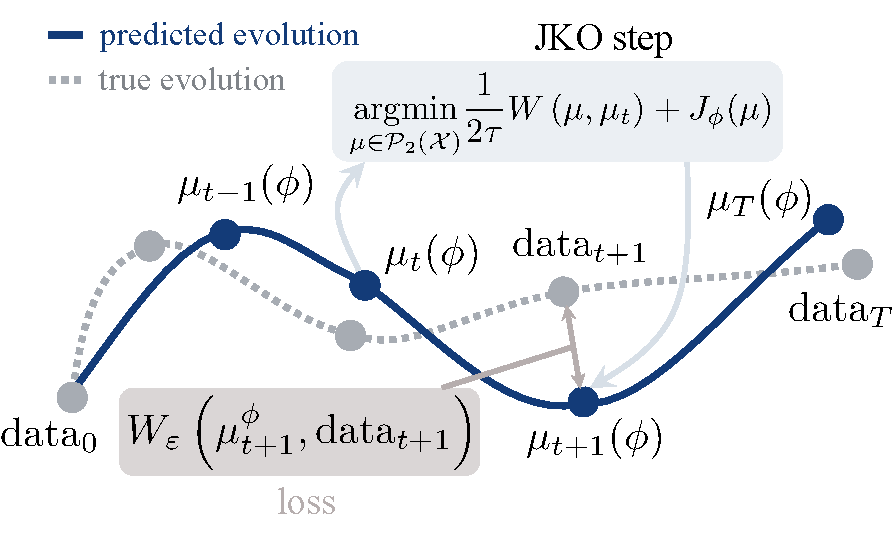
\includegraphics[width=0.6\textwidth]{figures/fig_overview_jkonet.pdf}
    \caption{Given an observed trajectory $(\mathrm{data}_0,\dots,\mathrm{data}_T)$ of point clouds (gray), we seek parameters $\xi$ for the energy $J_\xi$ such that the predictions $\mu_1, \dots, \mu_T$ (blue) following a \acrshort{JKO} flow from $\mu_0=\mu_0$ are close the observed trajectory (gray), by minimizing (as a function of $\xi$) the sum of Wasserstein distances between $\mu_{t+1}$, the \acrshort{JKO} step from $\mu_{t-1}$ using $J_\xi$, and data $\mu_{t+1}$.}
    \label{fig:overview_jkonet}
\end{figure}


\section{\textsc{JKOnet}: A Proximal Optimal Transport Model} 

Given $T$ discrete measures $\mathrm{data}_0, \dots, \mathrm{data}_T$ describing the time evolution of a population, we posit that such an evolution follows a \acrshort{JKO} flow for the free energy functional $J$, and assume that energy does not change throughout the dynamic. We parameterize the energy $J$ as a neural network with parameters $\xi$ and fit $\xi$ so that the \acrshort{JKO} flow model matches the observed data. 

Fitting parameter $\xi$ with a reconstruction loss requires, using the chain rule, being able to differentiate the \acrshort{JKO} step's output w.r.t. $\xi$ (see \cref{fig:overview_jkonet}), and more precisely provide a way to apply that transpose Jacobian to an arbitrary vector when using reverse-mode differentiation. To achieve this, we introduce a novel approach to numerically solve \acrshort{JKO} flows using \acrshortpl{ICNN} (\cref{sec:jko_icnn}), resulting in a bilevel optimization problem targeting the energy $J_\xi$ (\cref{sec:learn_energy}).

\subsection{Reformulation of JKO Flows via ICNNs} \label{sec:jko_icnn}
Given a starting condition $\mu_t$ and energy functional $J_\xi$, the \acrshort{JKO} step consists in producing a new measure $\mu_{t+1}$ implicitly defined as the minimizer of~\eqref{eq:jko}. Solving directly~\eqref{eq:jko} on the space of measures involves substantial computational costs. Different numerical schemes have been developed, e.g., based notably on Eulerian discretization of measures \citep{carrillo2021primal, benamou2016discretization}, and/or entropy-regularized optimal transport \citep{peyre2015entropic}. However, these methods are limited to small dimensions since the cost of discretizing such spaces grows exponentially. Except for the Eulerian approach proposed in \citep{peyre2015entropic}, obtained as the fixed point of a Sinkhorn-type iteration, the differentiation would also prove extremely challenging as a function of the energy parameter $\xi$.

\looseness=-1 To reach scalability and differentiability, we build upon the approach outlined in \citet{benamou2016discretization} to reformulate the \acrshort{JKO} scheme as a problem solved over convex functions, rather than on measures $\mu$. Effectively, this is equivalent to making a change of variables in~\eqref{eq:jko}: Introduce a (variable) convex function $\varphi$, and replace the variable $\mu$ by the variable $\nabla \varphi_{\sharp}\mu_t$. Writing
\begin{equation}\label{eq:en}
\begin{split}
\mathcal{E}_J(\mu, \nu) := J(\mu) +\frac{1}{2 \tau}W_2^2(\mu, \nu),\\
\end{split}
\end{equation}
this identity states that, assuming $\mu$ and $\nu$ being absolutely continuous w.r.t. Lebesgue measure that
$$\min_{\mu}\mathcal{E}_J(\mu,\nu) = \min_{\varphi \text{ convex}} \mathcal{F}_J(\varphi, \nu):= \mathcal{E}_J(\nabla \varphi_{\sharp}\nu, \nu)\,,$$
simplifying the Wasserstein term in \eqref{eq:en}, using the assumption that $\varphi$ is convex and \citeauthor{brenier1987decomposition}'s theorem \cref{thm:brenier}:
\begin{equation}\mathcal{F}_J(\varphi, \nu) = J(\nabla \varphi_{\sharp}\nu) +\frac{1}{2 \tau} \!\! \int\!\! \| x - \nabla \varphi(x) \|^2 d \nu(x)\label{eq:jko_psi}
\end{equation}

\begin{algorithm}[t]
\caption{\textsc{JKOnet}}
\label{algo:jkonet}
\begin{algorithmic}

   \STATE {\bfseries Input:} Dataset $\mathcal{D}=\{\{\mathrm{data}_t^0 \}_{t=0}^T, \ldots, \{\mathrm{data}_t^N \}_{t=0}^T\}$ of $N$ population trajectories, $\xi^0$ energy parameter initialization, $\theta^0$ ICNN parameter initialization, learning rates $\text{lr}_\theta$ and $\text{lr}_\xi$, step $\tau$, regularizer $\varepsilon$, tolerance $\alpha$, {\texttt{TeacherForcing}} flag
   \STATE {\bfseries Output:} Free energy $J_{\xi}$ explaining underlying population dynamics of snapshot data
   \smallskip
   
   \STATE $\xi\leftarrow \xi^0$
   \FOR{$\{\mathrm{data}_t\}_{t=0}^T \in \mathcal{D}$} 
   \FOR{$t \gets 0$ \textbf{to} $T-1$}

   \STATE $\theta\leftarrow \theta^0$

   \IF{\texttt{TeacherForcing} \textbf{or} $t=0$}
    \STATE $\nu \leftarrow \mathrm{data}_t$
   \ELSE
   \STATE $\nu \leftarrow \mu_t(\xi)$
   \ENDIF
   \WHILE{$\frac{\sum_i \norm{\nabla_{\theta_i}\mathcal{F}_{J_\xi}(\theta)}_2}{\sum_i \text{count}(\theta_i)} \ge \alpha$}
    
   \STATE $\theta \leftarrow \theta - \text{lr}_\theta \times \nabla_\theta \mathcal{F}_{J_\xi,\nu}(\theta)$
   \ENDWHILE
   \STATE $\mu_{t+1}(\xi) \leftarrow \nabla \varphi_{\theta \sharp} \nu$

   \STATE $\xi \leftarrow \xi - \text{lr}_\xi \times \nabla_\xi W_\varepsilon(\mu_{t+1}(\xi), \mathrm{data}_{t+1})$
   \ENDFOR
   \ENDFOR
	
\end{algorithmic}
\end{algorithm}

We pick an ICNN architecture to optimize over a restricted family of convex functions, $\{\varphi_{\theta}\}$, and define, starting from $\mu_0(\xi):=\mathrm{data}_0$, the recursive sequence for $t\geq 0$,
\begin{equation} \label{eq:next_pop}
\mu_{t+1}(\xi) := \nabla \varphi_{\theta^\star\!(\xi, \mu_t(\xi))\, \sharp}\, \mu_{t}(\xi)\,,
\end{equation}
with $\theta^\star(\xi, \mu_t)$ defined implicitly using $\xi$ and any $\nu$ as 
\begin{align} \label{eq:thetastar}
    \theta^\star(\xi, \nu):=\arg \min_{\theta} \mathcal{F}_J(\varphi_{\theta},\nu)
\end{align}

\paragraph{Strong convexity of $\varphi_\theta$.} The strong convexity and smoothness of a potential $\varphi$ impacts the regularity of the corresponding OT map $\nabla\varphi$ ~\citep{caffarelli2000monotonicity,figalli2010optimal}, since one can show that for a $\ell$-strongly convex, $L$-smooth $\varphi$ one has~\citep{paty2020regularity} that
$$
\ell \|x - y\| \leq \|\nabla\varphi(x) -\nabla\varphi(y)\|  \leq L\|x - y\|.
$$
While it is more difficult to enforce the $L$-smoothness of a neural network, and more generally its Lipschitz constants \citep{scaman2018lipschitz} it is easy to enforce its strong convexity, by simply adding a term $\ell \|x\|^2/2$ to the corresponding potential, or a residual rescaled term $\ell x$ to the output $\nabla\varphi(x)$. This approach can be used to enforce that the push-forward of the gradient of an ICNN does not collapse to a single point, maintaining spatial diversity.

\subsection{Learning the Free Energy Functional}  \label{sec:learn_energy}
The energy function $J_\xi : \mathcal{P}(\mathbb{R}^d) \rightarrow \mathbb{R}$ can be any parameterized function taking a measure as input. 
Since our model assumes that the observed dynamic is parameterized entirely by that energy (and the initial observation $\mu_0$), the more complex this dynamic, the more complex one would expect the energy $J_\xi$ to be. We focus in this first attempt on linear functions in the space of measures, that is expectations over $\mu$ of a vector-input neural network $E_\xi$
\begin{equation} \label{eq:energy}
    J_\xi(\mu) := \int E_\xi(x) d\mu(x),
\end{equation}
where $E_\xi:\mathbb{R}^d \rightarrow \mathbb{R}$ is a multi-layer perceptron (MLP).


Inferring nonlinear energies accounting for population growth and decline, as well as interactions between points, using the formalism of \citep{de2019stochastic}, transformers~\citep{vaswani2017attention} or set pooling methods \citep{edwards2016towards, zaheer2017deep}, is an exciting direction for future work.

To address slow convergence and instabilities for dynamics with many snapshots, we use teacher forcing \citep{williams1989learning} to learn $J_\xi$ through time. In those settings, during training, $J_\xi$ uses the ground truth as input instead of predictions from the previous time step. At test time, we do not use teacher forcing.

\subsection{Bilevel Formulation of \textsc{JKOnet}}
Learning the free energy functional $J_\xi$ while solving each \acrshort{JKO} step via an ICNN results in a challenging bilevel optimization problem.
At each time step, the predicted dynamics are compared to the ground truth trajectory $(\mathrm{data}_0, \mathrm{data}_1, \dots, \mathrm{data}_T)$ with the entropy-regularized OT loss (see \ref{eq:ot-reg}),
\begin{align} \label{eq:fittingloss}
\begin{split}
    \min_\xi & \sum_{t=0}^{T-1} W_\varepsilon(\mu_{t+1}(\xi), \mathrm{data}_{t+1}), \\
    \text{s.t. } & \mu_{0}(\xi) := \mathrm{data}_0, \\
      & \mu_{t+1}(\xi) := \nabla \varphi_{\theta^\star\, \sharp}\, \mu_{t}(\xi)\,, \\
      & \theta^\star:=\arg \min_{\theta} \mathcal{F}_{J_{\xi}}(\varphi_{\theta},\mu_t(\xi))
\end{split}
\end{align}
The dependence of the Sinkhorn divergence losses in \eqref{eq:fittingloss} on $\xi$ only appears in the fact that the predictions $\mu_{t+1}(\xi)$ are themselves implicitly defined as solving a \acrshort{JKO} step parameterized with the energy $J_\xi$. 

\begin{figure}[t]
    \centering
    %\vskip-0.1cm
    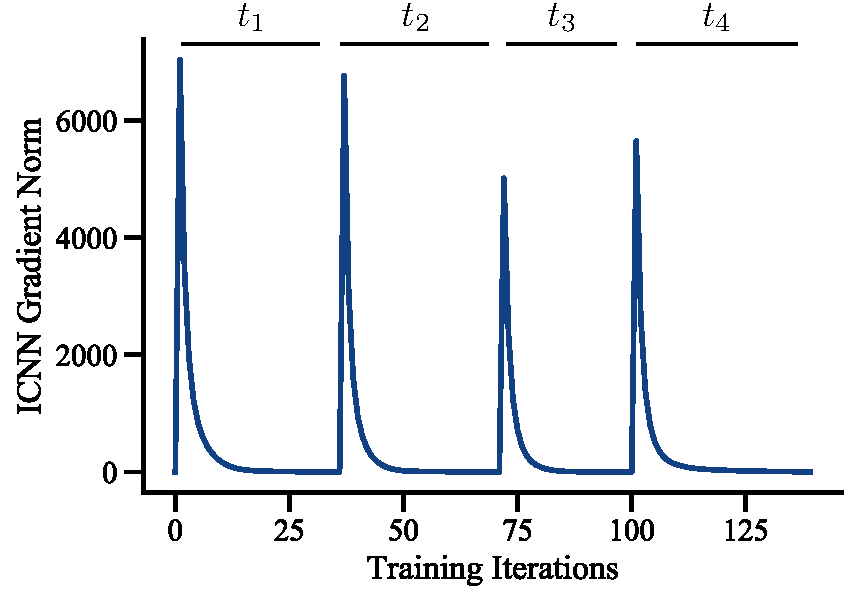
\includegraphics[width=.6\textwidth]{figures/fig_optimization_icnn.pdf}
    \caption{Optimization of the ICNN used in \acrshort{JKO} steps. The bumps correspond to a change in the outer iteration, and the smooth decrease in between corresponds to a single minimization~\eqref{eq:thetastar} of a time step $t_i$.}
    \label{fig:training_icnn}
\end{figure}

Learning  $J_\xi$ through the exclusive supervision of data observations requires therefore to differentiate the arg-minimum of a \acrshort{JKO} problem, down therefore through to the lower-level optimization of the ICNN. We achieve this by implementing a differentiable double loop in \texttt{JAX}, differentiating first the Sinkhorn divergence using the \texttt{OTT} package \citep{cuturi2022optimal}, and then backpropagating through the ICNN optimization by unrolling Adam steps \citep{kingma2014adam, metz2016unrolled, lorraine2020optimizing}.

\begin{figure*}[t]
\centering
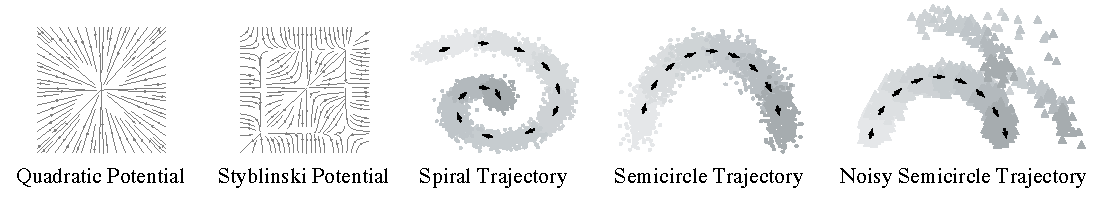
\includegraphics[width=1.0\textwidth]{figures/fig_task_overview_noise.pdf}
\caption{Overview on different tasks including trajectory- and potential-based dynamics.}
\label{fig:task_overview}
\end{figure*}

\paragraph{Inner loop termination.} A question that arises when defining $\mu_{t+1}(\xi)$ lies in the budget of gradient steps needed or allowed to optimize the parameters $\theta$ of the ICNN, before taking a new gradient step on $\xi$ in the outer loss. A straightforward approach in \texttt{JAX} \citep{jax2018github} would be to use a preset number of iterations with a \texttt{for} loop (\texttt{jax.lax.scan}). 
We do observe, however, that the number of iterations needed to converge in relevant scenarios can vary significantly with the ICNN architecture and/or the hardness of the underlying task.
We propose to use instead a differentiable fixed-point loop to solve each \acrshort{JKO} step up to a desired convergence threshold.
We measure convergence of the optimization of the ICNN via the average norm of the gradient of the \acrshort{JKO} objective w.r.t. the ICNN parameters $\theta$, i.e., $\sum_i \norm{\nabla_{\theta_i}\mathcal{F}_{J_\xi}(\theta_i, \xi)}_2/\sum_i \text{count}(\theta_i)$.
We observe that this approach is robust across datasets and architectures of the ICNN. An exemplary training curve for the \acrshortpl{ICNN} updated successively along a time sequence is shown in Figure~\ref{fig:training_icnn}.

\paragraph{Reverse-mode differentiation.} The Jacobian $\partial \mu_{t+1} / \partial\xi$ arising when computing the gradient $\nabla_\xi W_\varepsilon(\mu_{t+1}(\xi), \mathrm{data}_{t+1})$ is obtained by unrolling the while loop above. The gradient term of the Sinkhorn divergence w.r.t the first argument is given by the Danskin envelope theorem \citep{danskin2012theory}.

% The Jacobian $\partial \mu^\xi_{t+1} / \partial\xi$ that appears when computing $\nabla_\xi W_\varepsilon(\text{data}_{t+1}, \mu_{t+1}(\xi))$ is computed by unrolling the iterations of the while loop above.

\paragraph{Setting $\tau$ in \eqref{eq:jko_psi}.} 
In usual \acrshort{JKO} applications, $\tau$ needs to be tuned manually. Here, the energy $J_\xi$ is not fixed, but trained to fit data. Since we put no constraints on the scaling of $J_\xi$, $\tau$ can be set to $1$ without loss of generality, as the parameter $\xi$ will automatically adjust so that the scale of $J_\xi$ induces steps of a relevant length to fit data. This only holds (as with a usual \acrshort{JKO} step) if the trajectories are sampled regularly. For irregularly spaced time series, $\tau$ can be adapted at train and test time to the spacing of timestamps (shorter steps requiring larger $\tau$).


\begin{figure}[t]
     \centering
     \begin{subfigure}[t]{0.21\textwidth}
         \centering
         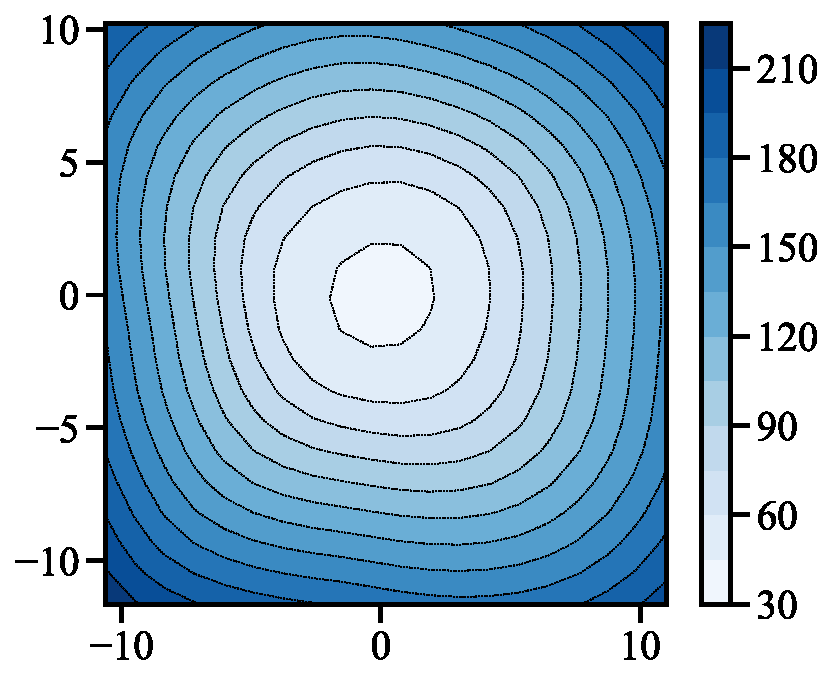
\includegraphics[width=\textwidth]{figures/fig_energy_implicit_quadratic.pdf}
         \caption{Quadratic \protect\newline Potential.}
     \end{subfigure}
     \hfill
     \begin{subfigure}[t]{0.21\textwidth}
         \centering
         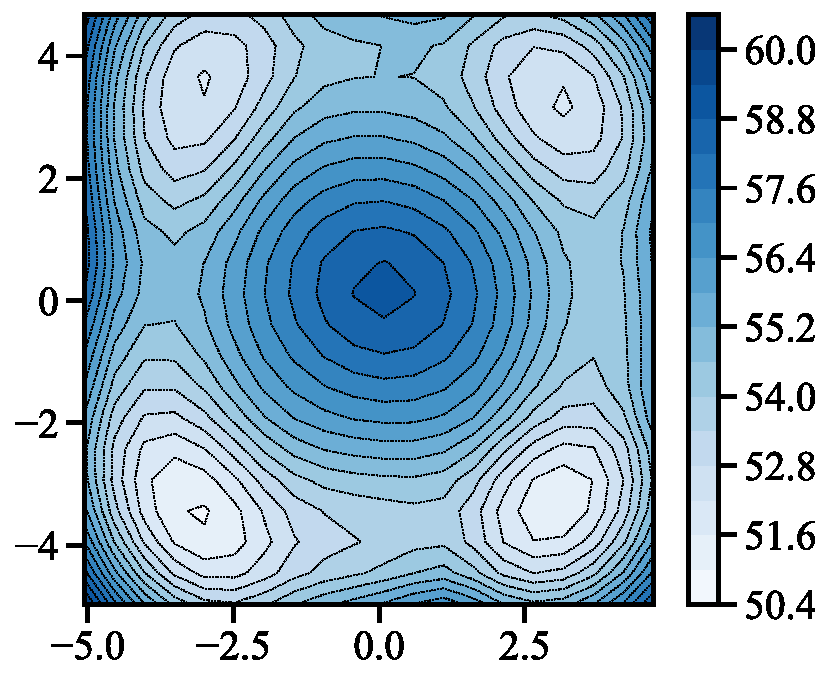
\includegraphics[width=\textwidth]{figures/fig_energy_implicit_styblinski.pdf}
         \caption{Styblinski \protect\newline Potential.}
     \end{subfigure}
     \hfill
     \begin{subfigure}[t]{0.22\textwidth}
         \centering
         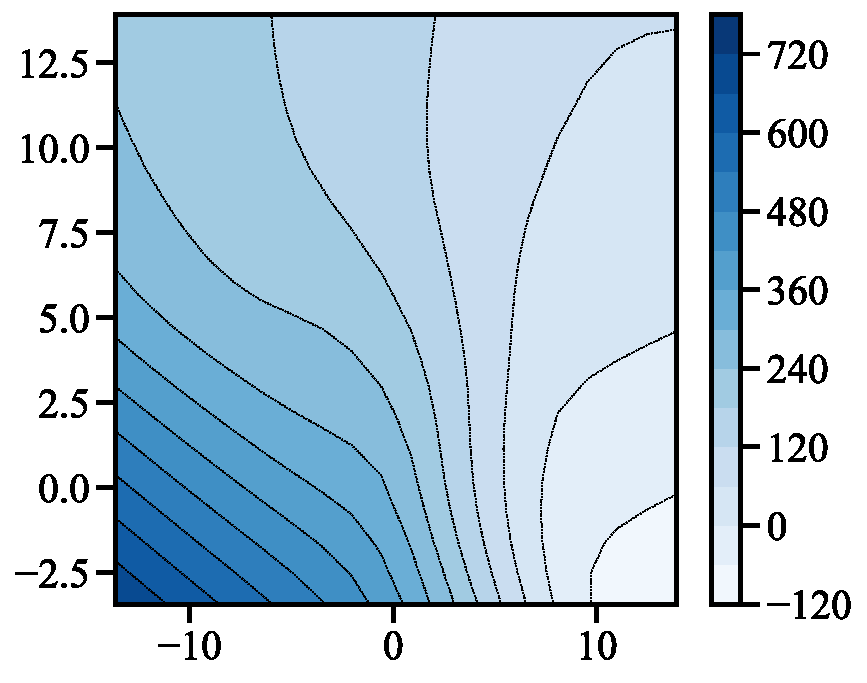
\includegraphics[width=\textwidth]{figures/fig_energy_implicit_semicircle_tf.pdf}
         \caption{Semicircle \protect\newline Trajectory.}
     \end{subfigure}
     \hfill
     \begin{subfigure}[t]{0.33\textwidth}
         \centering
         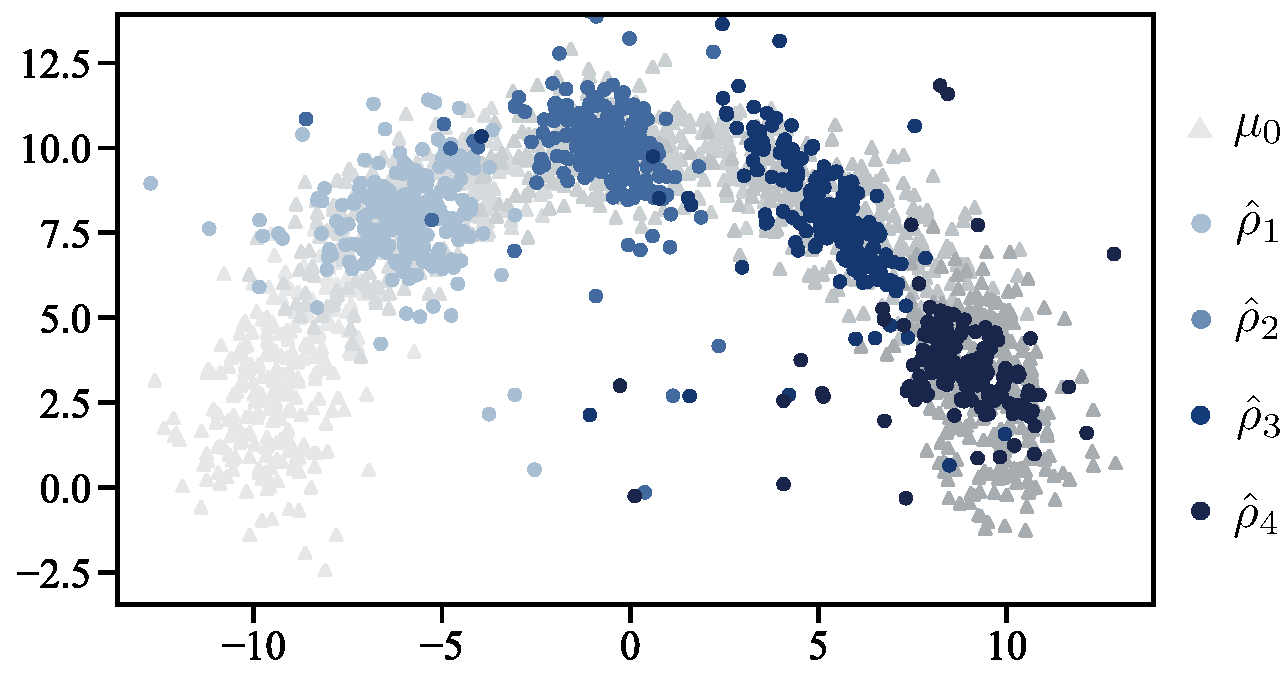
\includegraphics[width=\textwidth]{figures/fig_prediction_implicit_semicircle_tf.pdf}
         \caption{Predicted Evolution \protect\newline on Semicircle Trajectory.}
     \end{subfigure}
	 \caption{\textbf{Results of \textsc{JKOnet} on potential- and trajectory-based dynamics.} (a)-(c) Contour plots of the energy functionals $J_\xi$ of \textsc{JKOnet} on potential- and trajectory-based population dynamics, color gradients depict the magnitude of $J_\xi$. (d) Predicted population snapshots ($\mu_1, \dots, \mu_4$) (blue) and data trajectory ($\mathrm{d}_0, \dots, \mathrm{d}_4)$ (gray).}
	 \label{fig:exp_jkonet_pot_traj}
\end{figure}
\begin{figure}[t]
     \centering
     \begin{subfigure}[t]{0.24\textwidth}
         \centering
         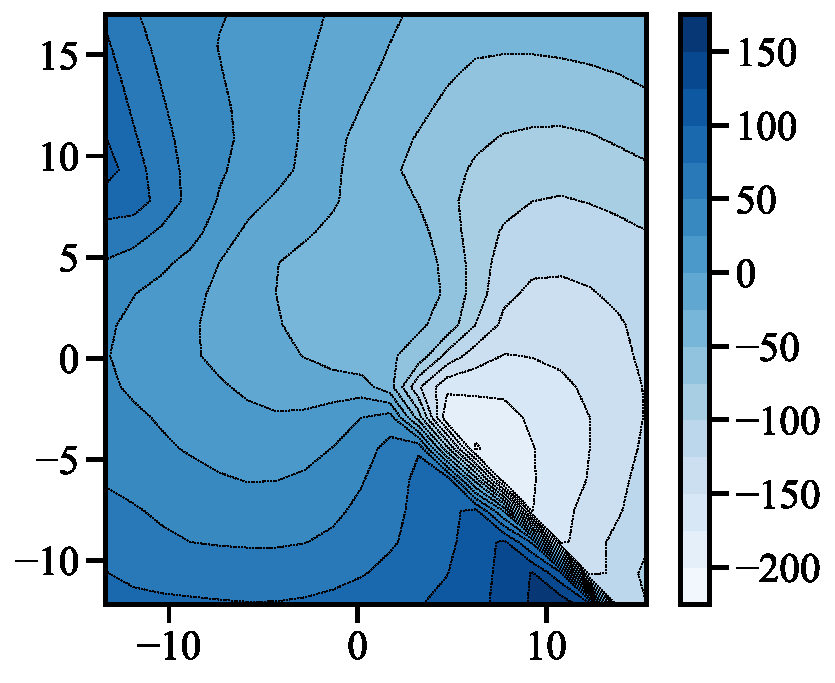
\includegraphics[width=\textwidth]{figures/fig_energy_explicit_spiral_tf.pdf}
         \caption{Forward method, \protect\newline teacher forcing.}
     \end{subfigure}
     \hfill
     \begin{subfigure}[t]{0.24\textwidth}
         \centering
         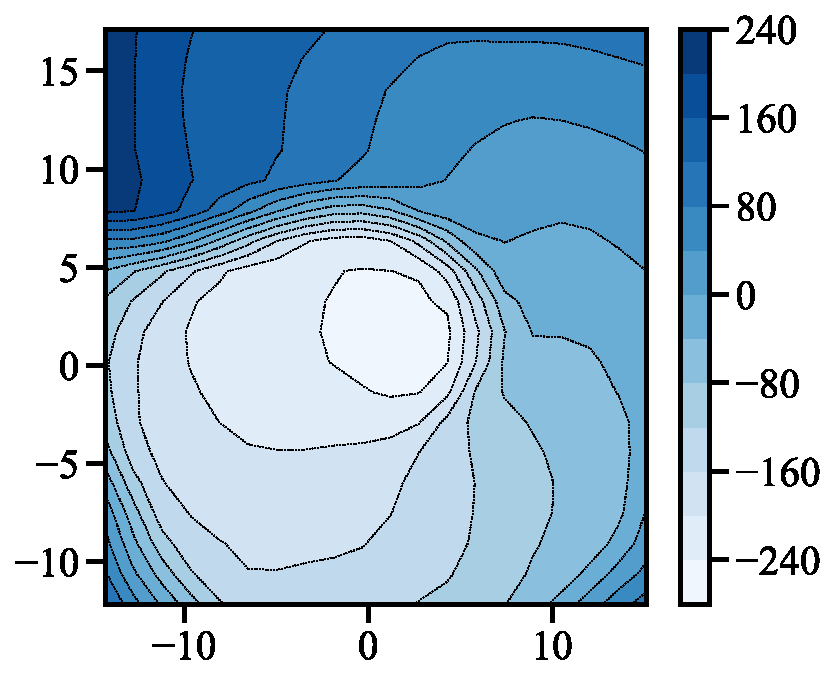
\includegraphics[width=\textwidth]{figures/fig_energy_explicit_spiral.pdf}
         \caption{Forward method, \protect\newline \emph{no} teacher forcing.}
     \end{subfigure}
     \hfill
     \begin{subfigure}[t]{0.24\textwidth}
         \centering
         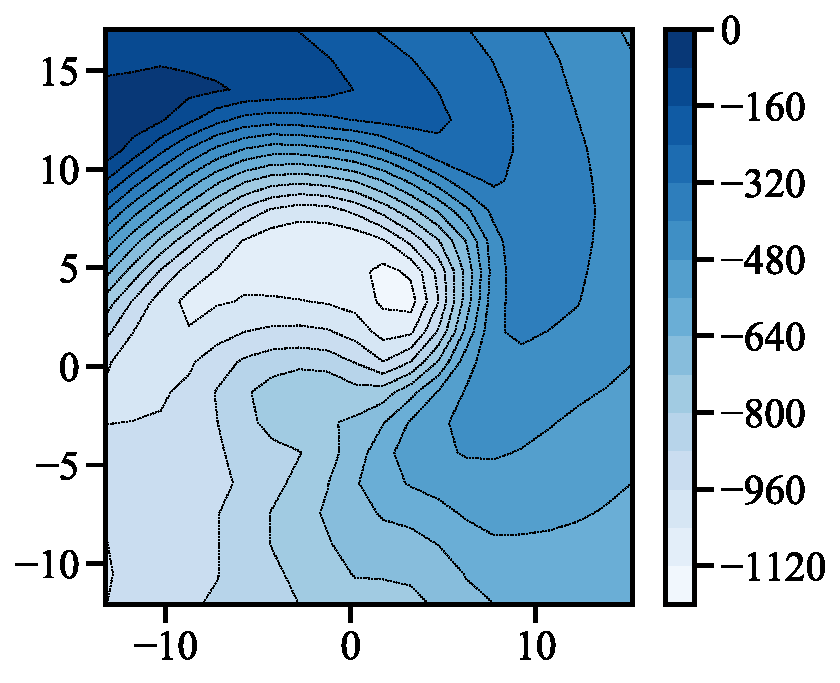
\includegraphics[width=\textwidth]{figures/fig_energy_implicit_spiral_tf.pdf}
         \caption{\textsc{JKOnet}, \protect\newline teacher forcing.}
     \end{subfigure}
     \hfill
     \begin{subfigure}[t]{0.24\textwidth}
         \centering
         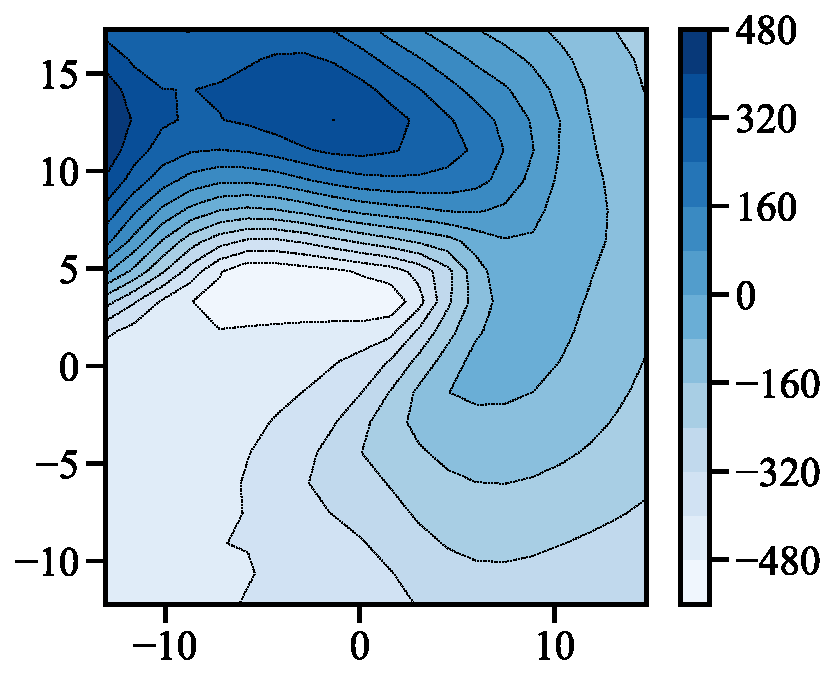
\includegraphics[width=\textwidth]{figures/fig_energy_implicit_spiral.pdf}
         \caption{\textsc{JKOnet}, \protect\newline \emph{no} teacher forcing.}
     \end{subfigure}
	 \caption{Comparison between energy functionals $J_\xi$ of the spiral trajectory task (see \ref{fig:task_overview}) between the forward method and \textsc{JKOnet}, trained with or without teacher forcing \cref{sec:learn_energy}). When using teacher forcing, the forward method overfits a gap in the lower-right corner of the spiral, outputting a highly irregular energy. When taking into account the entire trajectory recursively, the Forward method does better overall but is unable to recover an energy as precise as that returned by \textsc{JKOnet}.}
	 \label{fig:exp_comp_spiral}
\end{figure}

\begin{figure}[t]
     \centering
     \begin{subfigure}[b]{0.49\textwidth}
         \centering
         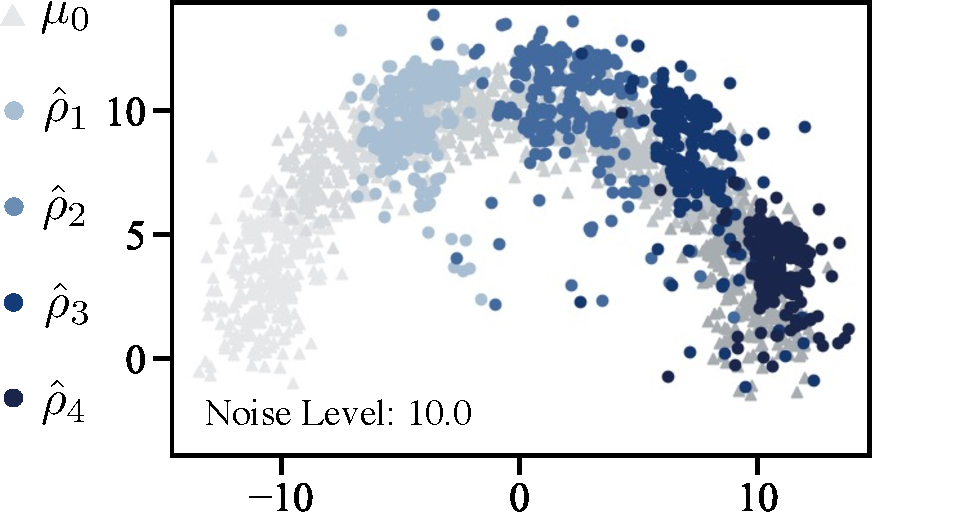
\includegraphics[width=\textwidth]{figures/fig_predictions_jko_noise.pdf}
         \caption{\textsc{JKOnet} (30\% corrupted data).}
     \end{subfigure}
     \hfill
     \begin{subfigure}[b]{0.47\textwidth}
         \centering
         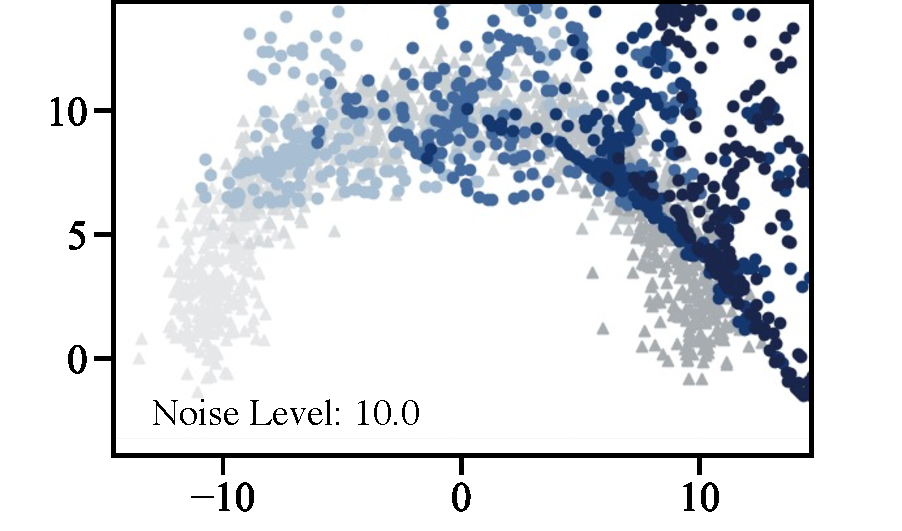
\includegraphics[width=\textwidth]{figures/fig_predictions_forward_noise.pdf}
         \caption{Forward method (30\% corrupted data).}
     \end{subfigure}
     
     \begin{subfigure}[t]{0.485\textwidth}
         \centering
         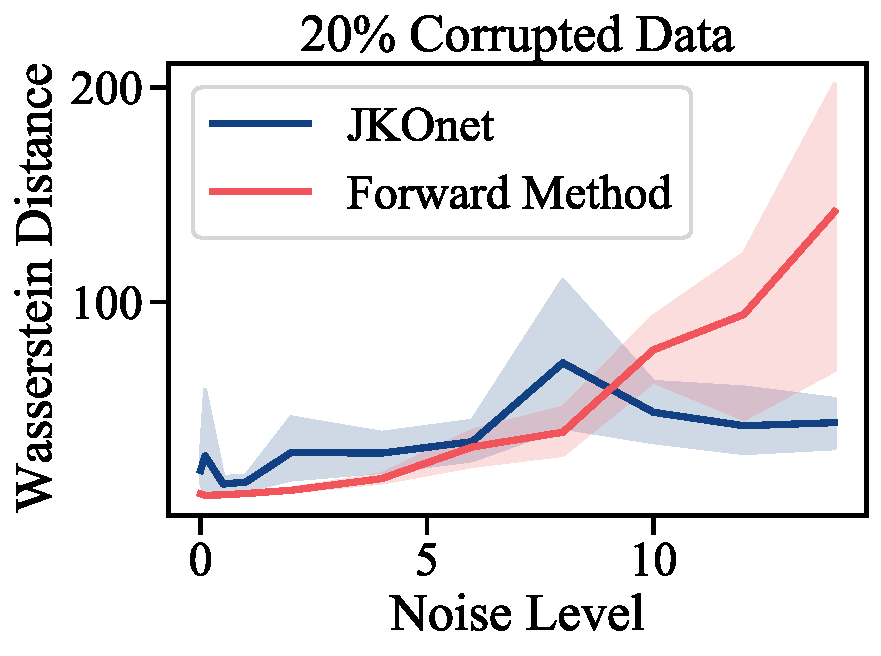
\includegraphics[width=\textwidth]{figures/fig_fb_comp_noise_20.pdf}
         \caption{$W_\epsilon$ vs. noise level (20\% corrupted data).}
     \end{subfigure}
     \hfill
     \begin{subfigure}[t]{0.46\textwidth}
         \centering
         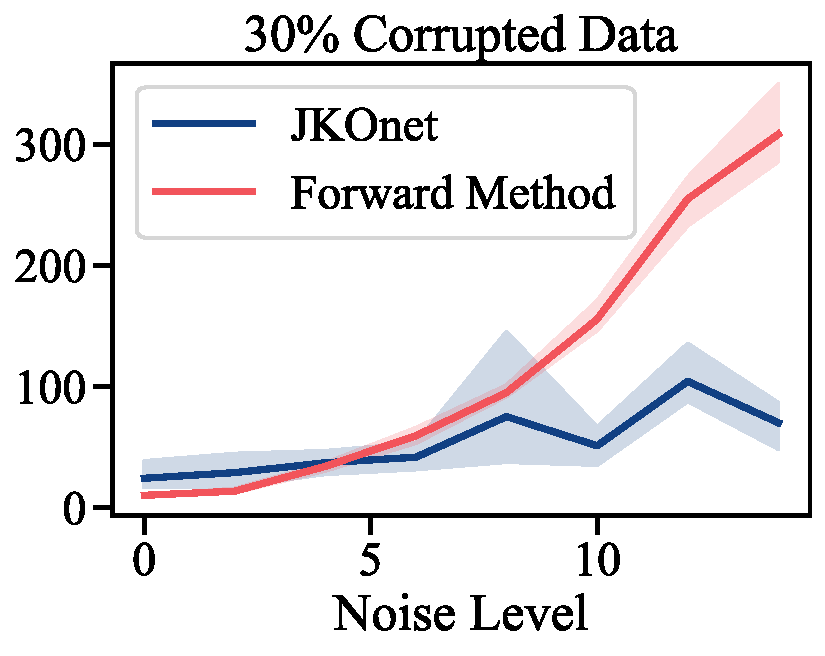
\includegraphics[width=\textwidth]{figures/fig_fb_comp_noise_30.pdf}
         \caption{$W_\varepsilon$ vs. noise level (30\% corrupted data).}
     \end{subfigure}
     \caption{Comparison between \textsc{JKOnet} and the forward method in settings of increasing noise on corrupted data on the semicircle trajectory task.}
     \label{fig:exp_comp_noise}
\end{figure}

\section{Empirical Evaluation} \label{sec:jkonet_evaluation}
In the following, we evaluate our method empirically on a variety of tasks. This includes recovering synthetic potential- and trajectory-based population dynamics (see \cref{fig:task_overview}), as well as the evolution of high-dimensional single-cell populations during a developmental process. 

\subsection{Synthetic Dynamics}
\label{sec:jkonet_synthetic}

\paragraph{Energy-driven trajectories.} The first task involves the evolution of partial differential equations with known potential. We hereby consider both convex (e.g., the quadratic function $J(x) = \|x\|^2_2$) and nonconvex potentials (e.g., Styblinski function) (see \cref{fig:task_overview}). These two-dimensional synthetic flows are generated using the Euler-Maruyama method~\citep{kloeden1992stochastic}. 
To recover the true potential via \textsc{JKOnet}, we parameterize both energy $J_\xi$ and ICNN $\varphi_\theta$ with linear layers ($\varepsilon = 1.0$, $\tau = 1.0$.
Figure~\ref{fig:exp_jkonet_pot_traj}a-b demonstrate \textsc{JKOnet}'s ability to recover convex and nonconvex potentials via energy $J_\xi$.

\paragraph{Arbitrary trajectories.}
As a sanity check, we evaluate if \textsc{JKOnet} can recover an energy functional $J_\xi$ from trajectories that are not necessarily arising from the gradient of an energy. Here, a 2-dimensional Gaussian moves along a predefined trajectory with nonconstant speed. 
We consider a line, a spiral, and movement along a semicircle (\cref{fig:task_overview}). As visible in Figure~\ref{fig:exp_jkonet_pot_traj}c (5 snapshots)], and Figure~\ref{fig:exp_comp_spiral}c-d (10 snapshots), \textsc{JKOnet} learns energy functionals $J_\xi$ that can then model the ground truth trajectories.
These trajectory-based dynamics are learned using the strong convexity regularizer ($\ell=0.8$, see \cref{sec:jko_icnn}).


\begin{table*}[t]
    \caption{Evaluation of predictive performance w.r.t. the entropy-regularized Wasserstein distance $W_\varepsilon$ \eqref{eq:ot-reg} of \textsc{JKOnet} and the forward method on the embryoid body scRNA-seq data per time step (using 3 runs).}
    \label{tab:exp_jkonet_cell_pred}
    \centering
\adjustbox{max width=.85\linewidth}{%
    \begin{tabular}{lcccc}
    \toprule
         \textbf{Method} & \multicolumn{4}{c}{\textbf{Prediction Loss ($W_\varepsilon$})} \\
         \cmidrule{2-5}
         & Day 6 to 9 & Day 12 to 15 & Day 18 to 21 & Day 24 to 27 \\
    \midrule
    \textbf{One Step Ahead} \\
        \tabindent Forward Method & $0.187 \pm 0.001$ & $0.162 \pm 0.010$ & $0.185 \pm 0.020$ & $0.203 \pm 0.004$ \\
        \tabindent \textsc{JKOnet} & $\mathbf{0.133 \pm 0.020}$ & $\mathbf{0.133 \pm 0.008}$ & $\mathbf{0.172 \pm 0.0130}$ & $\mathbf{0.169 \pm 0.004}$ \\
    \textbf{All Steps Ahead} \\
        \tabindent Forward Method & $0.225 \pm 0.023$ & $0.160 \pm 0.001$ & $0.171 \pm 0.016$ & $0.183 \pm 0.007$ \\
        \tabindent \textsc{JKOnet} & $\mathbf{0.148 \pm 0.015}$ & $\mathbf{0.144 \pm 0.013}$ & $\mathbf{0.154 \pm 0.024}$ & $\mathbf{0.138 \pm 0.034}$ \\
    \bottomrule
    \end{tabular}
}
\end{table*}

\paragraph{Comparison to forward methods.} \label{sec:eval_comp_fb}
Instead of parameterizing the next iteration $\mu_{t+1}(\xi)$ as we do in the \textsc{JKOnet} formulation~\eqref{eq:jko}, the \emph{forward} scheme states that the prediction at time $t+1$, $\eta_{t+1}$, can be obtained as $(\nabla F_\xi)_{\sharp} \eta_t(\xi)$, where $F_\xi$ is any arbitrary neural network, as considered in \citet{hashimoto2016learning}, namely $\eta_0:=\mu_0$ and subsequently $\eta_{t+1}(\xi):=(\nabla F_\xi)_{\sharp} \eta_t(\xi)$. Although OT still plays an important role in that paper, since the potential $F$ is estimated by minimizing a Sinkhorn loss $W_\varepsilon(\eta_{t+1},\mathrm{data}_{t+1})$, as we do in \eqref{eq:fittingloss}, the forward displacement operator $(\nabla F_\xi)_{\sharp}$ has no spatial regularity. Because of that, we observe that the forward method can get more easily trapped in local minima, and, in particular, overfits the training data as shown by a substantial decrease in performance in the presence of noise.
We demonstrate this by comparing the robustness of both \textsc{JKOnet} and the forward method to noise. For this, we corrupt $20\%$ or $30\%$ of the training data on the example of the semicircle trajectory with different levels of noise (see \cref{fig:task_overview}). We insist that noise is only added at training time, as random shifts on both feature dimensions, while we test on the original semicircle trajectory.
In low noise regimes, where train and test data are similar, the forward method overfits and performs marginally better than \textsc{JKOnet} (see \cref{fig:exp_comp_noise}c,d). As noise increases, the performance of the forward method deteriorates (\cref{fig:exp_comp_noise}b), while \textsc{JKOnet}, constrained to move points with OT maps, is robust (\cref{fig:exp_comp_noise}a).% This shows that the forward method is able to learn a network such that, on average, the ensemble of particles $(\nabla F_\xi)_{\sharp} \mu_t$ fits $\mu_{t+1}$, without, however

%In a second experiment, we evaluate the capacity of \textsc{JKOnet} and the forward method to extrapolate and generalize the learned trajectories, e.g., when vertically translating a line during test time (\cref{fig:task_overfitting}).
%Due to the less constrained energy, the \emph{forward} method perfectly resembles the seen trajectory during training but fails to extrapolate to shifted test data.

Second, we compare the resulting energy functionals $F_\xi$ and $J_\xi$ of the forward method and \textsc{JKOnet}, respectively, on the spiral trajectory (see \cref{fig:exp_comp_spiral}).
When learning long and complex population dynamics, teacher forcing improves training (see \cref{fig:exp_jkonet_pot_traj}c-d).
While facilitating the training of the forward method in some settings, it likewise results in wrong energy functionals $F_\xi$ (\cref{fig:exp_comp_spiral}a).
\textsc{JKOnet}, on the other hand, is able to globally learn the energy functional $J_\xi$, despite being only exposed to a one-step history of snapshots during training with teacher forcing (see \cref{fig:exp_comp_spiral}c).

\subsection{Single-Cell Dynamics}
\label{sec:jkonet_cell}

\begin{figure}[t]
     \centering
     \begin{subfigure}[t]{0.45\textwidth}
         \centering
         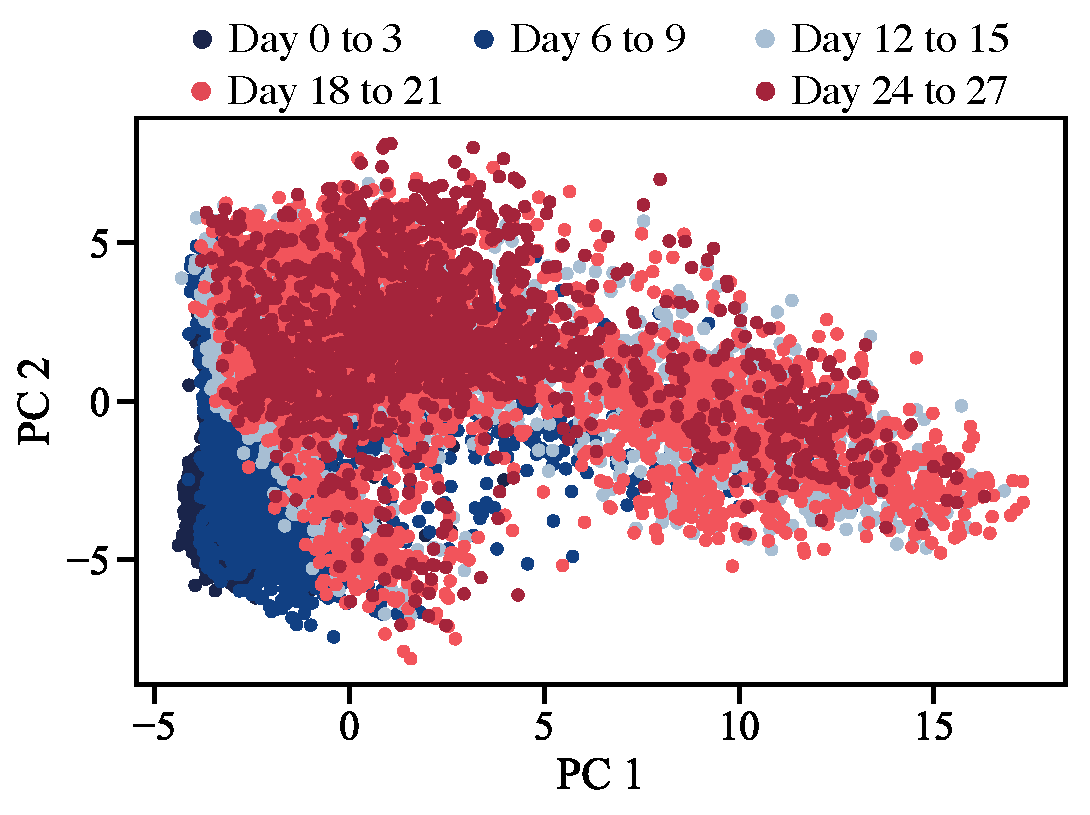
\includegraphics[width=\textwidth]{figures/fig_data_moon_days_full.pdf}
         \caption{\acrshort{PCA} embedding of the embryoid body scRNA-seq data colored by the snapshot time.}
     \end{subfigure}
     \hfill
     \begin{subfigure}[t]{0.45\textwidth}
         \centering
         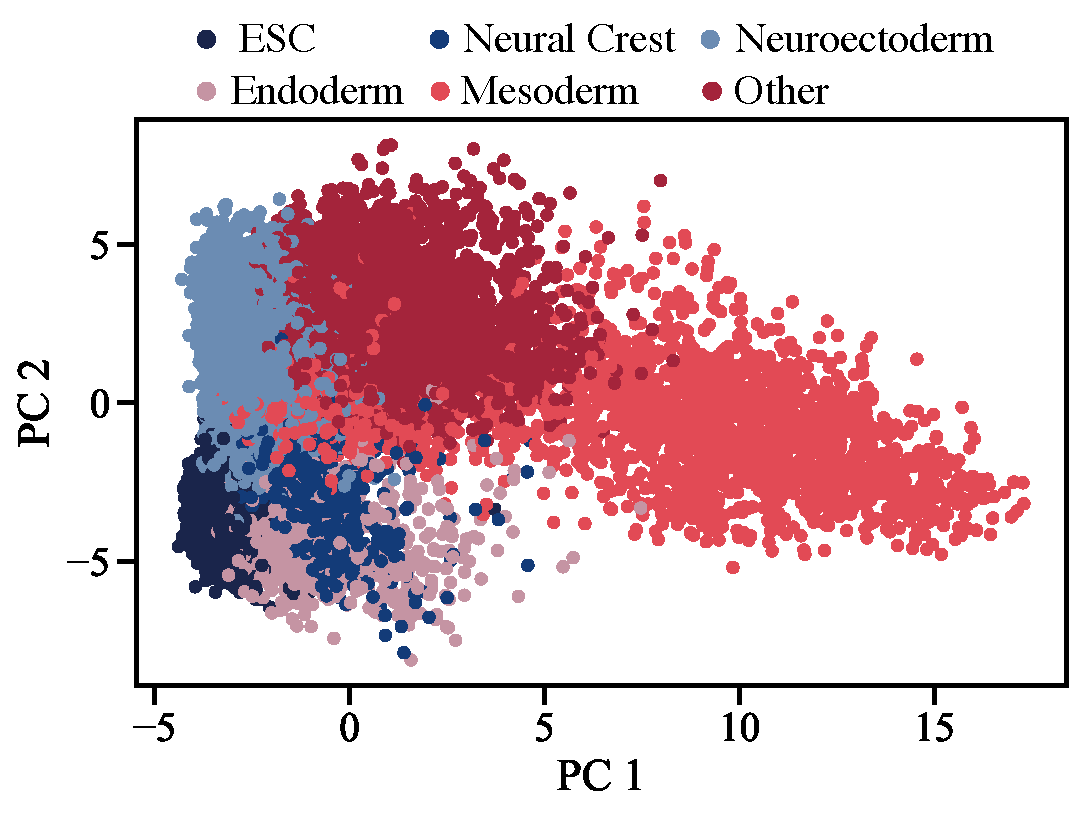
\includegraphics[width=\textwidth]{figures/fig_data_moon_Branches_full.pdf}
         \caption{\acrshort{PCA} embedding of the embryoid body scRNA-seq data colored by the lineage branch class.}
     \end{subfigure}

     \begin{subfigure}[t]{0.45\textwidth}
         \centering
         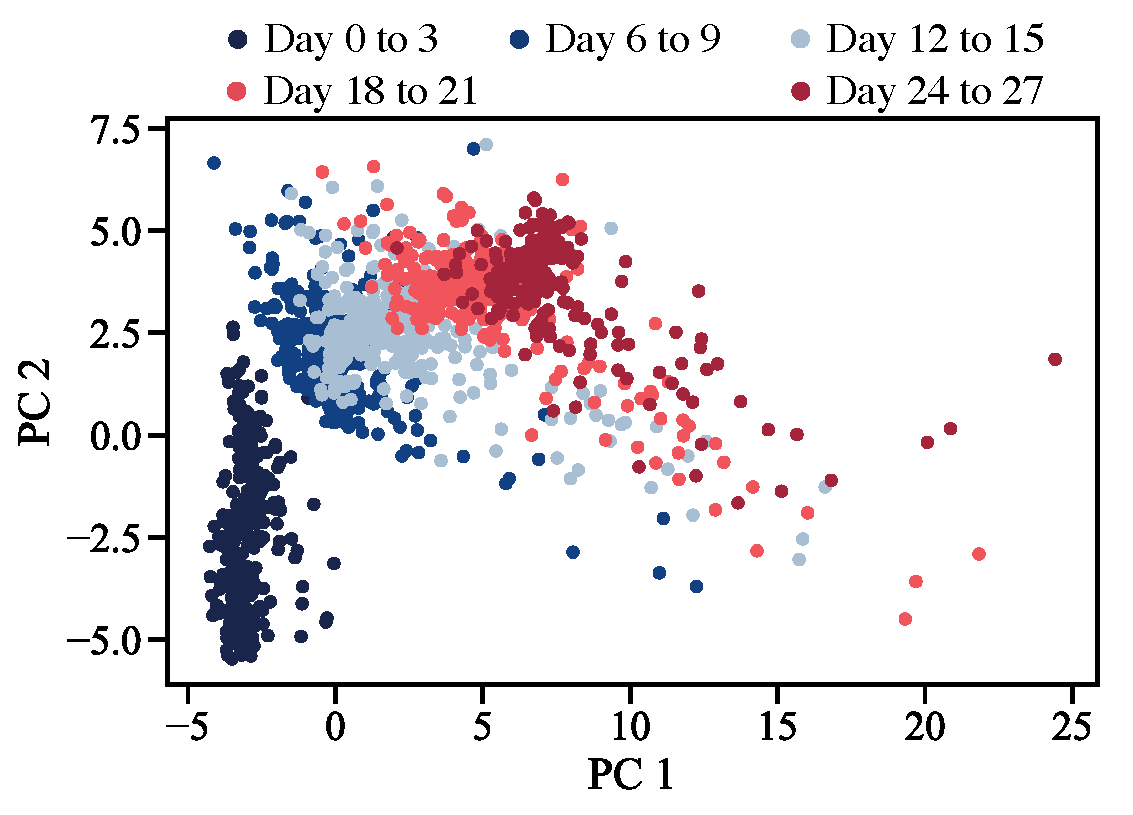
\includegraphics[width=\textwidth]{figures/fig_implicit_moon_pred_days.pdf}
         \caption{\acrshort{PCA} embedding of \textsc{JKOnet} predictions colored by the snapshot time.}
     \end{subfigure}
     \hfill
     \begin{subfigure}[t]{0.45\textwidth}
         \centering
         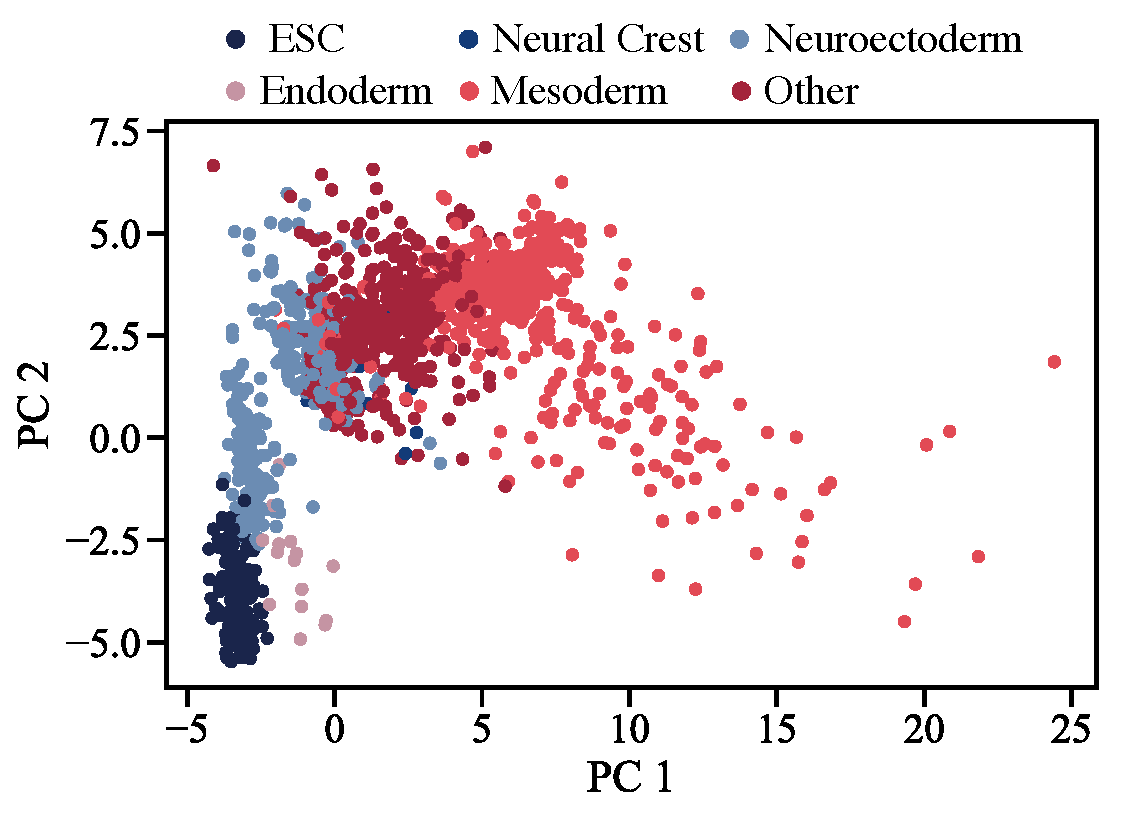
\includegraphics[width=\textwidth]{figures/fig_implicit_moon_pred_Branches.pdf}
         \caption{\acrshort{PCA} embedding of \textsc{JKOnet} predictions colored by the lineage branch class.}
     \end{subfigure}
	 \caption{Analysis of population dynamics predictions of \textsc{JKOnet} on the embryoid body scRNA-seq data.}
	 \label{fig:exp_jkonet_cell}
\end{figure}

\begin{figure}[t]
    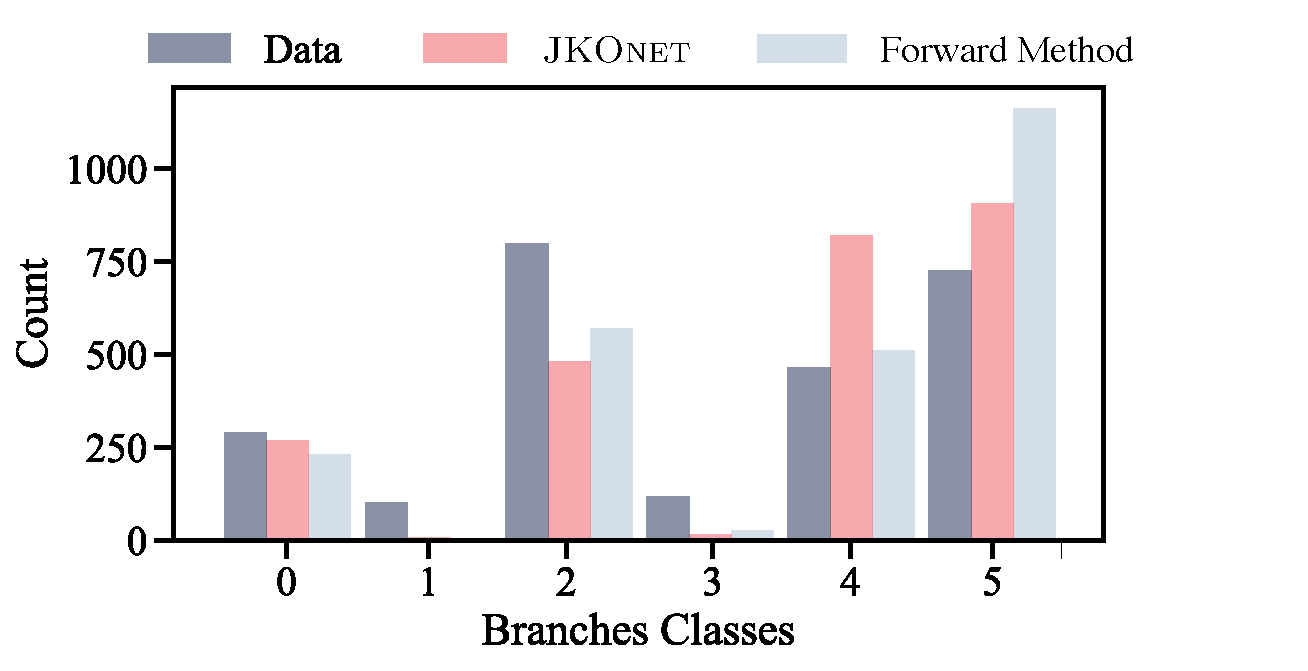
\includegraphics[width=.47\linewidth]{figures/fig_distribution_cell_types_Branches.pdf}
%    \captionof{figure}{Distribution of cell lineage branch classes in the data or  predicted by \textsc{JKOnet} or the forward method.}
	\qquad
	\resizebox{.45\linewidth}{!}{%
    \begin{tabular}[b]{lcc}
    \toprule
         \textbf{Method} & \multicolumn{2}{c}{\textbf{Cell Lineage Classification}} \\
         & $\ell_1$ & $H^2$ \\
    \midrule
    \textbf{One-Step Ahead} \\
        \tabindent Forward Method & $132.27 \pm 5.00$ & $0.026 \pm 0.002$ \\
        \tabindent \textsc{JKOnet} & $\mathbf{88.80 \pm 0.57}$ & $\mathbf{0.016 \pm 0.001}$ \\
    \textbf{All-Steps Ahead} \\
        \tabindent Forward Method & $\mathbf{185.47 \pm 12.18}$ & $0.033 \pm 0.002$ \\
        \tabindent \textsc{JKOnet} & $215.60 \pm 12.53$ & $0.034 \pm 0.004$ \\
    \bottomrule
    \end{tabular}
    }
\caption{Evaluation of cell lineage branch classification performance of \textsc{JKOnet} and the forward method on the embryoid body scRNA-seq data based on the $\ell_1$-distance of the histograms and the Hellinger distance $H^2$ \eqref{eq:hellinger} of the predicted branch class distributions (using 3 runs). \vspace{10pt}}
\label{tab:exp_jkonet_cell_class}
\end{figure}

We investigate the ability of \textsc{JKOnet} to predict the evolution of cellular and molecular processes through time.
The advent of single-cell profiling technologies has enabled the generation of high-resolution single-cell data, making it possible to profile individual cells at different stages in their development. 
A key difficulty in learning the evolution of cell populations is that a cell is (usually)  destroyed during a measurement. Thus, although one is able to collect features at the level of individual cells, the same cell cannot be measured twice. Instead, we collect independent samples at each snapshot, resulting in \emph{unaligned} distributions across snapshots, without access to ground-truth single-cell trajectories. 
The goal of learning individual dynamics is to identify ancestor and descendant cells and get a better understanding of biological differentiation or reprogramming mechanisms. 

We apply \textsc{JKOnet} to embryoid body single-cell RNA sequencing (scRNA-seq) data \citep{moon2019visualizing}, describing the differentiation of human embryonic stem cells grown as embryoid bodies into diverse cell lineages over a period of 27 days. During this time, cells are collected at 5 different snapshots (day 1 to 3, day 6 to 9, day 12 to 15, day 18 to 21, day 24 to 27) and measured via scRNA-seq (resulting in $15,150$ cells).
We run \textsc{JKOnet} as well as the baseline on the first 20 components of a \acrfull{PCA} of the $4,000$ highly differentiable genes.
We split the dataset into train and test data ($\sim 15 \%$) and parameterize both energy $J_\xi$ and ICNN $\varphi_\theta$ with linear layers ($\varepsilon = 1.0$, $\tau = 1.0$).

\paragraph{Capturing spatio-temporal dynamics.}
Given the samples from the cell population at day 1 to 3 (i.e., $\mathrm{data}_0$), \textsc{JKOnet} learns the underlying spatiotemporal dynamics giving rise to the developmental evolution of embryonic stem cells. 
As no ground truth trajectories are available in the data, we use distributional distances, i.e., the entropy-regularized Wasserstein distance $W_\varepsilon$ \eqref{eq:ot-reg} \citep{flamary2021pot}, to measure the correctness of the predictions at each time step.
We hereby measure the $W_\varepsilon$ discrepancy between data and predictions for one step ahead as well as inference of the entire evolution (all steps ahead) for each time step $t_i$, see results in Table~\ref{tab:exp_jkonet_cell_pred}. \textsc{JKOnet} outperforms the forward method in terms of $W_\varepsilon$ \eqref{eq:ot-reg} distance for both one-step ahead and all-steps ahead predictions for all time steps. 
The performance of both methods is relatively stable even until days 24 to 27, i.e., the $W_\varepsilon$ distance does not significantly grow for future snapshots.
We further visualize the first two principal components of the entire dataset (\cref{fig:exp_jkonet_cell}a) and of \textsc{JKOnet}'s predictions on the test dataset ($\sim 500$ cells per snapshot, \cref{fig:exp_jkonet_cell}d). 

\paragraph{Capturing biological heterogeneity.}
Besides measuring the ability of \textsc{JKOnet} to model and predict the spatiotemporal dynamics of embryonic stem cells, we would like to guarantee, at a more macroscopic level, that \textsc{JKOnet} is also able to learn the cell's differentiation into various cell lineages.
Embryoid body differentiation covers key aspects of early embryogenesis and thus captures the development of \acrlongpl{ESC} into the mesoderm, endoderm, neuroectoderm, neural crest, and others.

Following \citet[Fig. 6, Suppl. Note 4]{moon2019visualizing}, we compute lineage branch classes (\cref{fig:exp_jkonet_cell}b) for all cells based on an initial $k$-means clustering ($k=30$) in a 10-dimensional embedding space using PHATE, a non-linear dimensionality reduction method capturing a denoised representation of both local and global structure of a dataset.
We then train a $k$-nearest neighbor ($k$-NN) classifier ($k=5$) to infer the lineage branch class based on a 20-dimensional \acrshort{PCA} embedding of a cell (classes: ESC: 0, neural crest: 1, neuroectoderm: 2, endoderm: 3, mesoderm: 4, other: 5).

We analyze the captured lineage branch heterogeneity of the population predicted by \textsc{JKOnet} and the forward method by estimating the lineage branch class of each cell using the trained $k$-NN classifier. The predicted populations colored by the estimated lineage branch as well as the data with the true lineage branch labels are visualized in Figure~\ref{fig:exp_jkonet_cell}e and Figure~\ref{fig:exp_jkonet_cell}b, respectively.
The corresponding predicted and true distributions of lineage branch classes are shown in Figure~\ref{fig:exp_jkonet_cell}c.
To quantify how well \textsc{JKOnet} and the forward method capture  different cell lineage branches, we compute the $\ell_1$ distance between the  predicted and true histograms as well as the Hellinger distance 
\begin{equation} \label{eq:hellinger}
    H^2(a, b)=\frac{1}{2} \sum_{i=1}^{k}\left(\sqrt{a_{i}/\|a\|_1}-\sqrt{b_{i}/\|b\|_1}\right)^{2}
\end{equation}
between both true and predicted class discrete distributions $a$ and $b$.
Figure~\ref{fig:exp_jkonet_cell}c and Table~\ref{tab:exp_jkonet_cell_class} demonstrate that both, \textsc{JKOnet} and the forward method, capture most lineage branches during the differentiation of embryonic stem cells. Both methods, however, have difficulties recovering cells of the neural crest (class 1) and the endoderm (class 3), lineage branches that are scarcely represented in the original data. 
The analysis further suggests that both methods reduce in performance w.r.t. biological heterogeneity when predicting the entire trajectory (all steps ahead), instead of inferring the next snapshot only (one step ahead).


\section{Discussion}
We proposed \textsc{JKOnet}, a model to infer and predict the evolution of population dynamics using a proximal optimal transport scheme, the \acrshort{JKO} flow.
\textsc{JKOnet} solves local \acrshort{JKO} steps using \acrshortpl{ICNN} and learns the energy that parameterizes these steps by fitting \acrshort{JKO} flow predictions to observed trajectories using a fully differentiable bilevel optimization problem.
We validate its effectiveness through experiments on synthetic potential- and trajectory-based population dynamics and observe that it is far more robust to noise than a more direct Forward approach. We use \textsc{JKOnet} to infer the developmental trajectories of human embryonic stem cells captured via high-dimensional and time-resolved single-cell RNA-seq. 
Our analysis also shows that \textsc{JKOnet} captures diverse cell fates during the incremental differentiation of embryonic cells into multiple lineage branches.
Using proximal optimal transport to model real complex population dynamics thus makes for an exciting avenue of future work. Extensions could include modeling higher-order interactions among population particles in the energy function, e.g., cell-cell communication.

\chapter[Learning Dynamical Systems via OT and Stochastic Control]{Learning Dynamical Systems via Optimal Transport and Stochastic Control}
\label{cha:neural_sde}

\dictum[Erwin Schr{\"o}dinger, \textit{What is Life?} (1944)]{%
  Living matter evades the decay to equilibrium.}%
\vskip 2em

\verpar{Contributions}{
Most of the material in this chapter has been already published in the following conference proceedings:
\begin{itemize}
	\item[] Charlotte Bunne, Ya-Ping Hsieh, Marco Cuturi, and Andreas Krause. The Schr{\"o}dinger Bridge between Gaussian Measures has a Closed Form. In \textit{International Conference on Artificial Intelligence and Statistics (AISTATS)}, 2023.
	\item[] Vignesh Ram Somnath, Matteo Pariset, Ya-Ping Hsieh, Maria Rodriguez Martinez, Andreas Krause, and Charlotte Bunne. Aligned Diffusion Schr{\"o}dinger Bridges. In \textit{Conference on Uncertainty in Artificial Intelligence (UAI)}, 2023.
	\vspace{-9pt}
\end{itemize}
}

One of the main challenges in continuously modeling cellular dynamics concerns the innate randomness and fluctuations that exist in biological systems.
These random events, such as the timing of a gene being transcribed, or the inherent noise in protein production, make cellular dynamics inherently stochastic.
Stochastic processes provide an apt mathematical framework to encapsulate these random phenomena.
They enable us to model not just a smoothed behavior, but also the variance and distribution of outcomes, and thus allow us to capture rare but biologically significant events.
Therefore, modeling cellular dynamics as stochastic processes is essential to capture the full spectrum of biological behaviors and understand the underlying mechanisms driving these intricate processes. 

Consequently, the following chapter deals with the question of learning and identifying a stochastic process $\mathbb{P}_t$ that describes the evolution of a population $\mu_0$ at time point $t=0$ into a population $\mu_T$ at time $t=T$.
To draw parallels to \cref{cha:bio_background}, $\mu_0$ and $\mu_T$ potentially represent gene expression samples of cells at time $0$ and $T=\horizon$. In this context, recovering the dynamics from $\mathbb{P}_0 = \distinit$ to $\mathbb{P}_1 = \distend$ might provide us with an understanding of how and why tumor cells evade cancer therapies \citep{frangieh2021multimodal} or to reconstruct developmental trajectories \citep{schiebinger2019optimal}.

More concretely, the following chapter concerns \acrlongpl{SB}, a framework that combines the theory of \acrlong{OT} with stochastic optimal control formulations (see \cref{sec:background_sb}) and identifies a stochastic process $\mathbb{P}_t$ that represents the evolution of a thermodynamic system at almost equilibrium.

The chapter is divided into two parts: 
\cref{sec:gsbflow} builds on the realization that estimating such bridges is notoriously difficult. Here, we hypothesize that Gaussian approximations of the data can be used to construct a data-driven reference stochastic process needed to estimate \acrshort{SB}. To that end, we solve the \acrshort{SB} problem with Gaussian marginals, for which we provide, as a central contribution, a closed-form solution and \acrshort{SDE} representation. We use these formulas to define the reference process used to estimate more complex \acrshortpl{SB} and show that this does indeed help with its numerical solution.

\cref{sec:sbalign} similarly proposes a new training objective for learning and parameterizing \acrshortpl{SB} by utilizing the structure of \emph{aligned} data, which naturally arises in many biological phenomena.
While most \acrlong{sc} measurement technologies are destructive (see \cref{sec:tech_background}), recent developments in molecular biology aim at overcoming this technological limitation. For example, \citet{chen2022live} propose a transcriptome profiling approach that preserves cell viability. \citet{weinreb2020lineage} clonal tracing evolving cells, allowing us to connect them to their progenitors.
Here we propose a novel algorithmic framework that, for the first time, learns \acrshortpl{SB} while respecting the data alignment hinging on a combination of two decades-old ideas: The classical \acrlong{SB} theory and Doob's \emph{$h$-transform}.

\section{Diffusion Schr{\"o}dinger Bridges}
\label{sec:background_dsb}

As described above, in order to learn the evolution of a population from $\mu_0$ to $\mu_1$, we will invoke the framework of \acrshortpl{SB}.
Given two marginals $\distinit$ and $\distend$, we select a reference process $\refpro$ based on prior knowledge, for instance, simple \acrlong{BM}. As discussed in \cref{sec:background_sb}, it turns out that  the solution to the general \acrshort{SB} problem \eqref{eq:schrodinger_bridge} is itself given by two coupled \acrshortpl{SDE} \eqref{eq:sb_forward}-\eqref{eq:sb_backward} \citep{leonard2013survey}, which we restate here for convenience
\begin{eqnarray}
\label{eq:SB-sde-forward}
\dsde &= \parens*{\tdriftbase +  \volatbase \SBfbase_\ctime} \dt + \volatbase \dWiener[\ctime],\quad \sde[0] \sim \distinit, \\ % \; & \sde[0] \sim \Pinit, \\
\label{eq:SB-sde-backward}
\dsde &= \parens{\tdriftbase -  \volatbase \SBbbase_\ctime} \dt + \volatbase \dWiener[\ctime],\quad \sde[\horizon] \sim \distend\,, % \; & \sde[\horizon] \sim \Pend.
\end{eqnarray}
where we replaced $\nabla \log \Phi\left(t, X_t\right)$ in \eqref{eq:sb_forward} and $\nabla \log \widehat{\Phi}\left(t, X_t\right)$ in \eqref{eq:sb_backward} with $\SBfbase_\ctime, \SBbbase_\ctime \from \R^\vdim \to \R^\vdim$, i.e., two time-indexed smooth \emph{vector fields} called the optimal forward and backward drift, respectively. Note that \eqref{eq:SB-sde-backward} runs backward in time, i.e., from $\horizon \to 0$ \citep{anderson1982reverse}. % and satisfies many interesting properties \citep{nelson1967dynamical, leonard2013survey, chen2021stochastic}.
Choosing $f$ and $g$ depending on the considered \acrshort{SDE} class, the forward and backward policies $\SBfbase_\ctime, \SBbbase_\ctime$ are generally \emph{unknown}.
Similar as in \acrlongpl{SGM} \citep{song2020score, hyvarinen2005estimation} which parameterize the score function, in order to \emph{estimate} the resulting \acrshort{SB} from data, we learn the forward and backward drift through \acrlongpl{NN} with parameters $\paramf, \paramb$, i.e., $\SBf$ and $\SBb$. For a visualization of the resulting parameterization, see \cref{fig:principle_dsb}. \\

\begin{figure}[t]
	\centering
	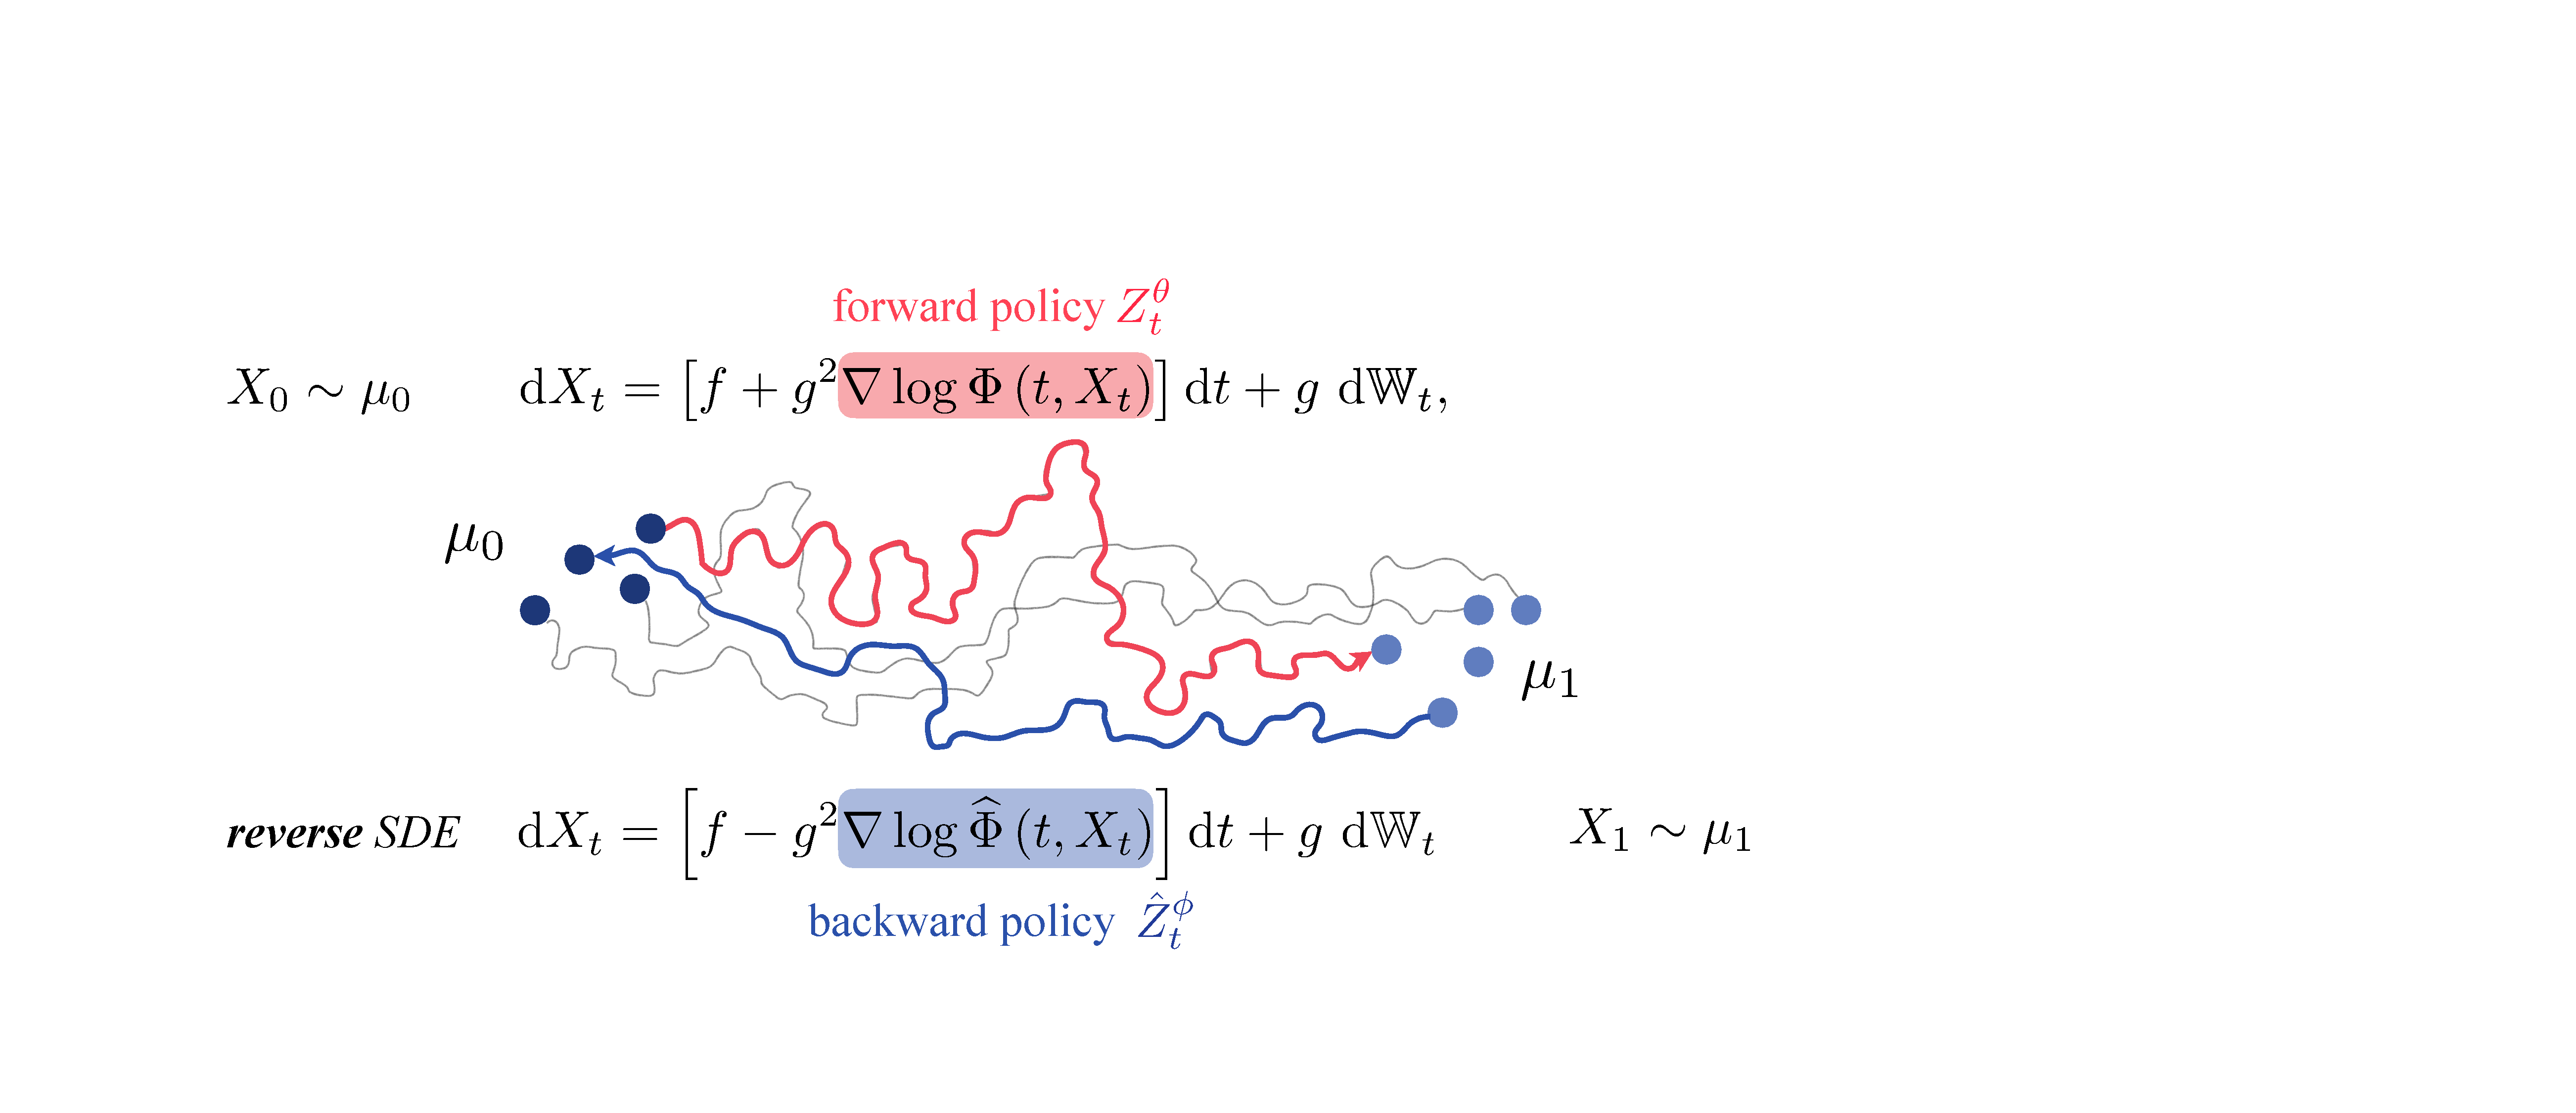
\includegraphics[width=0.8\textwidth]{figures/fig_principle_dsb.pdf}
	\caption{\textbf{Parameterization of \acrlongpl{DSB}.} The forward \acrshort{SDE} with forward policy {\color{pink} $\SBfbase_\ctime$} steers particles $X_0 \sim \mu_0$ from $t=0$ to $\mu_1$ at $t=1$. The reverse \acrshort{SDE} runs backward in time. Here, backward policy {\color{blue} $\SBbbase_\ctime$} determines the evolution of particles $X_1 \sim \mu_1$ at $t=1$ to $\mu_0$ at $t=0$.} 
	\label{fig:principle_dsb}
\end{figure}

Several estimators and training procedures for the so-called \acrlongpl{DSB}, i.e., for learning $\SBfbase_\ctime$ and $\SBbbase_\ctime$, have been proposed based on either Gaussian processes \citep{vargas2021solving}, dual potentials \citep{finlay2020learning}, or \acrlongpl{NN} \citep{de2021diffusion, chen2021likelihood}.
In this thesis, we consider the likelihood training framework by \citet{chen2021likelihood} grounded on \acrfull{FBSDE} theory \citep{ma1999forward, exarchos2018stochastic}. Crucially, these \acrshortpl{FBSDE} can be used to construct the likelihood objectives for \acrshortpl{SB} that, surprisingly, generalize the ones for \acrshortpl{SGM} as special cases. 

The negative likelihood functions for $\paramf$ and $\paramb$ are then given by
\begin{subequations}
\begin{align}
\lossb =  \int_0^\horizon \mathbb{E}_{\eqref{eq:SB-sde-forward}}\Big[ \frac{1}{2}\norm{\SBbbase^{\paramb}_\ctime}^2 &+\volatbase \Div \SBbbase^{\paramb}_\ctime+ \inner{\SBfbase^{\paramf}_\ctime}{\SBbbase^{\paramb}_\ctime} \dt \Big\vert \sde[0] = \point_0 \Big] ,  \\
\lossf =  \int_0^\horizon \mathbb{E}_{\eqref{eq:SB-sde-backward}}\Big[ \frac{1}{2}\norm{\SBfbase^{\paramf}_\ctime}^2 &+\volatbase \Div \SBfbase^{\paramf}_\ctime + \inner{\SBbbase^{\paramb}_\ctime}{\SBfbase^{\paramf}_\ctime} \dt \Big\vert \sde[\horizon] = \point_{\horizon} \Big].
\end{align}
\end{subequations}
and serve as loss functions for likelihood-based training of \acrshortpl{DSB}. Here, $\Div$ denotes the divergence operator w.r.t. the $\point$ variable: For any $v\from \R^\vdim \to \R^\vdim$, $\Div v(\point) \defeq \sum_{\coord=1}^{\vdim} \ddc v_\coord(\point)$.

Unfortunately, such frameworks necessitate a forward-backward learning process known as the \acrfull{IPF} procedure \citep{fortet1940resolution, kullback1968probability}.
As both policies $\SBfbase_\ctime, \SBbbase_\ctime$ are initially unknown and randomly parameterized, training \acrshortpl{DSB} often results in numerical and scalability issues.

Further, none of these approaches is capable of incorporating \emph{alignment} of the data. This can be seen by inspecting the objective \eqref{eq:schrodinger_bridge}, in which the coupling information $(\x_0^i,\x_1^i)$ is completely lost as only its individual marginals $\distinit,\distend$ play a role therein.  

In this chapter, we tackle both of these limitations: First, in \cref{sec:gsbflow} we derive a data-driven reference process that provides a more robust initialization of \acrshortpl{DSB}. Second, in \cref{sec:sbalign}, we devise the first algorithmic framework that solves \eqref{eq:SB-sde-forward}-\eqref{eq:SB-sde-backward} in settings where sparse trajectories, or partially aligned data, are available \emph{without} resorting to \acrshort{IPF}.

\section{Data-Driven Priors for Diffusion Schr{\"o}dinger Bridges} \label{sec:gsbflow}

The \acrlong{SB} \citep{leonard2013survey, chen2021stochastic}, alternatively known as the \emph{dynamic} entropy-regularized \acrlong{OT}, has recently received significant attention from the machine learning community. In contrast to the classical \emph{static} \acrshort{OT} where one seeks a coupling between measures that minimizes the average cost \citep{villani2009optimal,peyre2019computational}, the goal of \acrshortpl{SB} is to find the optimal \emph{stochastic processes} that evolve a given measure into another. As such, \acrshortpl{SB} are particularly suitable for learning complex continuous-time systems and have been successfully applied to a wide range of applications such as sampling \citep{bernton2019schr, huang2021schrodinger}, generative modeling \citep{chen2021likelihood,de2021diffusion,wang2021deep}, molecular biology \citep{holdijk2022path}, and mean-field games \citep{liu2022deep}. 

% The \emph{static} \acrlong{OT} (OT) problems seek to find the optimal mapping which transforms a given probability measure into another while minimizing the 

% Comparing between probability measures is ubiquitous in machine learning, for which 
% \Acrlong{OT} and entropy-regularized \acrshort{OT} problems play a pivotal role in machine learning \citep{villani2009optimal, peyre2019computational}, where one seeks a \emph{mapping} that transports between measures while minimizing the average cost. In recent years, there is a rapid growth of interest in solving the \emph{dynamical} extensions of these \acrshort{OT} problems, i.e., finding the optimal \emph{trajectories} that transport measures, with applications ranging from sampling and generative modeling to molecular dynamics and mean-field games. In the literature, these dynamical \acrshort{OT} problems are known as the \acrlong{SB} \citep{leonard2013survey, chen2021stochastic} due to an equivalent formulation that dates back to \citep{schrodinger1931umkehrung, schrodinger1932theorie}.

% the dynamic extensions of these \acrshort{OT} problems, i.e., finding the optimal \emph{trajectories} that transport measures have witnessed a sudden surge of interest. A particularly prominent instance of these extensions is the \acrlong{SB} \citep{schrodinger1931umkehrung, schrodinger1932theorie}, for comparing constrained \emph{stochastic processes} has attracted significant attention. Creative applications of \acrshort{SB} have already yielded success in sampling and generative modeling tasks, while also witnessing a surging interest in fields like molecular dynamics and mean-field games. 

Despite these impressive achievements, a common limitation of the existing works is that the \acrshortpl{SB} are typically solved in a purely {numerical} fashion. In sharp contrast, it is well-known that many important \acrshort{OT} problems for \emph{Gaussian} measures admit \emph{closed-form} solutions, and the advantages of such solutions are numerous: they have inspired new learning methods \citep{rabin2011wasserstein, vayer2019sliced, bonneel2015sliced}, they can serve as the ground truth for evaluating numerical schemes \citep{janati2020entropic}, and they have lead to the discovery of a new geometry that is both rich in theory and application \citep{takatsu2010wasserstein}. 

\begin{figure}[t]
    \centering
    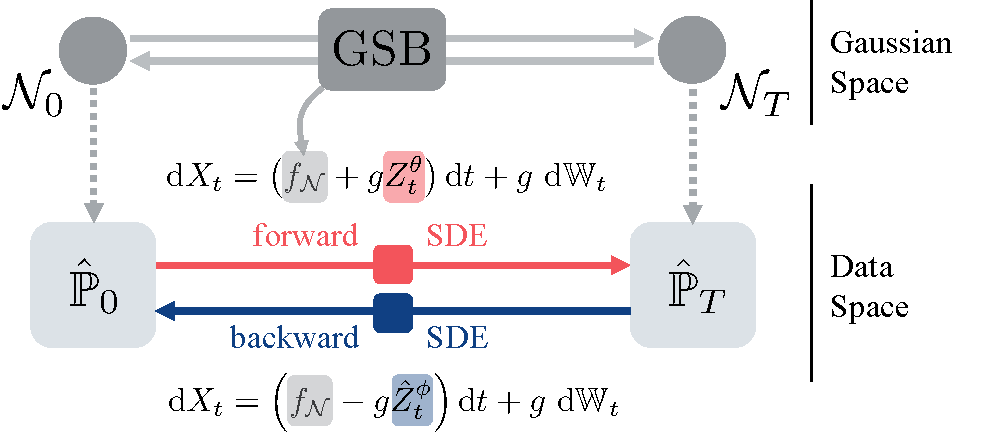
\includegraphics[width=0.7\textwidth]{figures/fig_overview_gsb.pdf}
    \caption{Solving the \acrshort{SB} problem between $\distinit$ and $\distend$ is notoriously difficult because it requires learning the time-dependent drifts of two SDEs that respect the desired marginals, and a random initialization for these drifts is usually extremely far from satisfying that constraint. We propose a data-dependent procedure that relies first on Gaussian approximations of the data measures, which provide a closed-form drift $f_{\mathcal{N}}$ in \eqref{eq:GSB-forward} (the \acrshort{GSB}). We show that this facilitates the training of forward/backward drifts $\hat{Z}^\theta_t, \hat{Z}^\phi_t$.}
    \label{fig:overview_gsbflow}
\end{figure}

The goal of this section is to continue this pursuit of closed-form solutions and extend these advantages to \acrshort{SB}-based learning methods. For an overview of the method, see \cref{fig:overview_gsbflow}. To this end, we make the following contributions: \\

%As a central contribution, we derive a set of new expressions for \acrfullp{GSB}, i.e.,\acrshortpl{SB} between Gaussian measures, that covers a wide range of applications. Furthermore, our analysis reveals a
\begin{enumerate}[leftmargin=.4cm,itemsep=.0cm,topsep=.0cm]
\item As our central result, we derive the closed-form expressions for \acrfullpl{GSB}, i.e., \acrshortpl{SB} between Gaussian measures. This is a challenging task for which all existing techniques fail, and thus we need to resort to a number of new ideas from entropic \acrshort{OT}, Riemannian geometry, and generator theory; see \cref{sec:overview_gsbflow}.
% These formulas constitute the first non-trivial closed forms for \emph{dynamic} entropy-regularized \acrshort{OT}. %The proof combines a number of ideas from entropic \acrlong{OT}, Riemannian geometry, Gaussian analysis, and generator theory, which might be of independent interest.

\item We extend the deep connection between geometry and Gaussian \acrshort{OT} to \acrlongpl{GSB}. In particular, our results can be seen as a vast generalization of the classical Bures-Wasserstein geodesics between Gaussian measures \citep{takatsu2010wasserstein, bhatia2019bures}, which is the foundation of many computational methods \citep{chewi2020gradient, altschuler2021averaging, han2021riemannian}.

\item Via a simple Gaussian approximation on real \emph{\acrlong{sc} genomics} data, we numerically demonstrate that many benefits of the closed-form expressions in static \acrshort{OT} immediately carry over to \acrshort{SB}-based learning methods: We report improved numerical stability and tuning insensitivity when trained on benchmark datasets, which ultimately lead to overall better performance.
\end{enumerate}

\subsection{Preliminaries on Gaussian Optimal Transport}
\label{sec:prelim_gsbflow}

Throughout this chapter, let $\xi \sim \Ncal(\mu, \Sigma)$ and $\xi' \sim \Ncal(\mu', \Sigma')$ denote two given Gaussian random variables. By abusing the notation, we will continue to denote the measures of these Gaussians by $\xi$ and $\xi'$, respectively. We will also denote by $\Pi(\xi,\xi')$ the set of all their couplings. 

\subsubsection{Static Gaussian Optimal Transport}
\label{sec:staticGOT}

The \emph{static} entropy-regularized \acrshort{OT} between Gaussians refers to the following minimization problem \citep{peyre2019computational}:
% An important class of problems which generalizes \eqref{eq:W2Gaussian}, is the static entropy-regularized \acrshort{OT} between Gaussians:
\begin{equation}
\label{eq:RegW2Gaussian}
%\tag{OT$_\sigma$}
\min_{\coupling \in \Coupling(\xi, \xi')} \int  \norm{\point-\pointalt}^2  \drm \coupling(\point, \pointalt) + 2\sigma^2 \KL(\pi \| \xi \otimes \xi'),
\end{equation}where $\xi\otimes\xi'$ denotes the product measure of $\xi$ and $\xi'$, and $\sigma \geq 0$ is a regularization parameter. When $\sigma = 0$, \eqref{eq:RegW2Gaussian} reduces to the classical 2-Wasserstein distance between $\xi$ and $\xi'$ \citep{villani2009optimal}, whose closed-form solution is classical \citep{dowson1982frechet, olkin1982distance}. The case for general $\sigma$ is more involved, and an analytical expression was only recently found \citep{bojilov2016matching, del2020statistical, janati2020entropic, mallasto2021entropy}: Setting% the specific form is quite convoluted, and thus we defer it to \cref{app:gaussian_sb}.
\begin{equation}
\label{eq:Cstar}
D_\sigma \defeq \parens{ 4\Sigma^{\frac{1}{2}} \Sigma' \Sigma^{\frac{1}{2}} + \sigma^4\eye  }^{\frac{1}{2}},\quad C_\sigma \defeq \frac{1}{2}\parens{\Sigma^{\frac{1}{2}} D_\sigma \Sigma^{-\frac{1}{2}} - \sigma^2\eye},
\end{equation}
then the solution $\pi^\star$ to \eqref{eq:RegW2Gaussian} is itself a Gaussian:
\begin{align}
\label{eq:StaticGaussianSB-sol}
\pi^\star \sim \Ncal \parens*{  \begin{bmatrix}
\mu \\
\mu'
\end{bmatrix},  \begin{bmatrix}
\Sigma&C_\sigma\\
C_\sigma^T &\Sigma'
\end{bmatrix}}.
\end{align}

\subsubsection{Dynamic Gaussian Optimal Transport}
\label{sec:dynamicGOT-BB}

% TODO: Homogenize v_t notation to Background chapter.
In the literature, \eqref{eq:RegW2Gaussian} is commonly referred to as the \emph{static} \acrshort{OT} formulation since it merely asks \emph{where} the mass should be transported to (i.e., $\pi(\point,\pointalt)$ dictates how much mass at $\point$ should be transported to $\pointalt$). In contrast, the more general problem of \emph{dynamic} Gaussian \acrshort{OT} seeks to answer \emph{how} the mass the should be transported:
\begin{align}
\label{eq:BBGaussian}
\min_{\ssstyle\substack{{\measure[0] = \xi,\ \measure[\horizon] = \xi'}}} \exof*{\int_{0}^\horizon  \frac{1}{2} \norm{\vect}^2 + \frac{\sigma^4}{8} \norm*{\nabla\log\measure}^2 \dt}.
\end{align}Here, the minimization is taken over all pairs $(\measure, \vect)$ where $\measure$ is an absolutely continuous curve of measures \citep{ambrosio2006gradient}, and $\vect:\R^\vdim\to\R^\vdim$ is such that the continuity equation holds:
\begin{equation}
\label{eq:Coneq}
\pt\measure = - \Div(\measure \vect),
\end{equation}
where $\left(\Div \vect\right)(\point) \coloneqq \sum_{i=1}^d \frac{\partial}{\partial \point_i}v^{i}(\point)$ denotes the divergence operator with respect to the $\point$ variable. It can be shown that if $\measure^\star$ is the optimal curve for \eqref{eq:BBGaussian}, then the joint distribution of the end marginals $(\measurebase^\star_0, \measurebase_1^\star)$ coincides with \eqref{eq:StaticGaussianSB-sol}, hence the interpretation of $\measure^\star$ as the optimal \emph{trajectory} in the space of measures  \citep{chen2016relation, gentil2017analogy, chen2021stochastic, gentil2020dynamical}.

To our knowledge, the only work that has partially addressed the closed-form solution of \eqref{eq:BBGaussian} is \citet{mallasto2021entropy}, whose results are nonetheless insufficient to cover important applications such as generative modeling. In \cref{sec:results_gsbflow}, we will derive a vast generalization of the results in \citet{mallasto2021entropy} and provide a detailed comparison in \crefrange{sec:overview_gsbflow}{sec:mechanics_gsbflow}.


\subsection{The Gaussian Schr{\"o}dinger Bridge Problem}
\label{sec:overview_gsbflow}


The purpose of this section is to introduce the core objectives of this part of the thesis, i.e., the \acrlongpl{GSB}, and establish their connection to the Gaussian \acrshort{OT} problems in \cref{sec:prelim_gsbflow}. To help the reader navigate our somewhat technical proofs in \crefrange{sec:mechanics_gsbflow}{sec:results_gsbflow},  we illustrate in \cref{sec:tere} the high-level challenges as well as our new techniques for solving \acrlongpl{GSB}.

\subsubsection{Schr{\"o}dinger Bridges as Dynamic Entropy-Regularized Optimal Transport}


Let $\nu, \nu'$ be two given measures, and let $\refpro$ be an arbitrary stochastic process. In its most generic form, the \acrlong{SB} refers to a constrained KL-minimization problem overall stochastic processes $\Pmargin$ \eqref{eq:schrodinger_bridge} \citep{leonard2013survey, chen2021stochastic}, which we extensively discussed in \cref{sec:background_sb} and restate here for convenience:
\begin{equation}
\label{eq:SB}
\tag{SB}
\min_{ \substack{ \Pinit = \nu, \; \Pend = \nu'} } \KL(\Pmargin \|\refpro).% \quad \sigma >0 \textup{ and \Wiener
\end{equation}
In practice, $\nu$ and $\nu'$ typically arise as the (empirical) \emph{marginal} distributions of complicated continuous-time dynamics observed at the starting and end times, and $\refpro$ is a ``prior process'' representing our belief of the dynamics before observing any data. The solution $\Pstar$ to \eqref{eq:SB} is thus interpreted as the best dynamics that conforms to the prior belief $\refpro$ while respecting the data marginals ($\Pstar[0] = \nu, \Pstar[\horizon] = \nu'$). 

We will consider a general class of $\refpro$'s that includes most existing processes in the machine learning applications of \acrshortpl{SB}. Specifically, with some initial condition $\refsde[0]$, we will take $\refpro$ to be the measure of the linear \acrlong{SDE}:
% To facilitate the numerical solutions of \eqref{eq:SB}, $\refpro$ is typically chosen so that conditional distributions given initial points admit a simple expression. To this end, we will consider the following general class of \acrlongpl{SDE} which incorporates, to our knowledge, all the existing processes in the literature: With some initial condition $\refsde[0]$, take $\refpro$ to be the measure of
\begin{equation}
\label{eq:linearsde}
\drefsde = \parens*{\drift \refsde  + \shift }\dd t + \volat \dWiener[\ctime] \defeq \driftf\dt + \volat \dWiener[\ctime].
\end{equation}
Here, $\drift: \R^+ \to \R$, $\shift : \R^+ \to \R^\vdim$, and $\volat: \R^+ \to \R^+$ are smooth functions. In this case, \acrshortpl{SB} can be seen as generalized dynamical \acrshort{OT} between two (not necessarily Gaussian) measures:
%it is well-known that \eqref{eq:SB} can be seen as a generalized Benamou-Brenier \acrshort{OT} for two arbitrary (not necessarily Gaussian) measures \citep{chen2016relation, gentil2017analogy}:
\begin{theorem}
\label{thm:gsbtobb}
Consider the \acrlong{SB} problem with $\refsde$ as the reference process: 
\begin{equation}
\label{eq:YtSB}
%\tag{$\refsde$-SB}
\min_{ \substack{ \Pinit = \nu, \; \Pend = \nu'} } \KL(\Pmargin \|\refsde).% \quad \sigma >0 \textup{ and \Wiener
\end{equation}
Then \eqref{eq:YtSB} is equivalent to
\begin{align}
\label{eq:dynamicGSB}
&\inf_{(\measure,\vect)} \mathbb{E}\Bigg[\int_0^\horizon  \frac{\norm{\vect}^2}{2\volatsq[\ctime]} + \frac{\volatsq[\ctime]}{8} \norm{\nabla \log \measure}^2  - \frac{1}{2} \inner{\driftf}{\nabla \log\measure} \dt\Bigg]
\end{align}where the infimum is taken all pairs $(\measure,\vect)$ such that $\measure[0] = \nu, \measure[\horizon] = \nu'$, $\measure$ absolutely continuous, and
\begin{align}
\label{eq:Coneq2}
\partial_t \measure = -\Div \parens*{  \measure\parens*{ \driftf + \vect}  }.
\end{align}
\end{theorem}
The proof of \cref{thm:gsbtobb}, which we defer to \cref{app:gsbtobb}, is a straightforward extension of the argument in \citep{leonard2013survey, chen2016relation, gentil2017analogy} which establishes the equivalence when $\refsde$ is a reversible \acrlong{BM}, i.e., $\driftf \equiv0, \volat[\ctime] \equiv \sigma,$ and $\refsde[0]$ follows the Lebesgue measure.\footnote{The reversible \acrlong{BM} is a technical construct to simplify the computations. For our purpose, one can think of $\refsde[0]\sim \xi$ instead of the Lebesgue measure, and our results still hold verbatim.}  


\subsubsection{The Gaussian Schr{\"o}dinger Bridge Problem}
\label{sec:tere}

The central goal of this section is to derive the closed-form solution of \acrshortpl{SB} when the marginal constraints are Gaussians $\xi \sim \Ncal(\mu, \Sigma),\ \xi' \sim \Ncal(\mu', \Sigma')$. Namely, we are interested in the following class of the \acrshortpl{SB}, termed \acrlongpl{GSB}:% refers to the KL-minimization problem:
\begin{equation}
\label{eq:GSB}
\tag{GSB}
\min_{ \substack{ \Pinit = \xi, \; \Pend = \xi'} } \KL( \Pmargin \| \refsde).% \quad \sigma >0 \textup{ and \Wiener
\end{equation}
To emphasize the dependence on the reference \acrshort{SDE}, we will sometimes call \eqref{eq:GSB} the $\refsde$-\acrshort{GSB}. 


%In view of \cref{thm:gsbtobb}, $\refsde$-\acrshortpl{GSB} are 
%When $\refsde = \variance \Wiener$, 
% $\mathbb{P}^\star_{0,1} = \pi^\star$ 
%
%General reference processes

%\subsubsection{Technical Challenges and Related Work} 
%\label{sec:tere}

\paragraph{Technical challenges and related work.} In order to analyze \eqref{eq:GSB}, we first notice that the objective in \eqref{eq:dynamicGSB} becomes $\sigma^{-2}\exof*{\int_{0}^\horizon  \frac{1}{2} \norm{\vect}^2 + \frac{\sigma^4}{8} \norm*{\nabla\log\measure}^2 \dt}$ for $\sigma\Wiener$-\acrshortpl{GSB}. Up to a constant factor, this is simply \eqref{eq:BBGaussian}, so \cref{thm:gsbtobb} reduces to the well-known fact that $\sigma\Wiener$-\acrshortpl{GSB} are a reformulation of the dynamic Gaussian \acrshort{OT} \citep{leonard2013survey, chen2016relation, gentil2017analogy}. 

At first sight, this might suggest that one can extend existing tools in Gaussian \acrshort{OT} to analyze \acrshortpl{GSB}.%\eqref{eq:BBGaussian} to \eqref{eq:dynamicGSB}.
~Unfortunately, the major difficulty of tackling \acrshortpl{GSB} is that these existing tools are fundamentally insufficient for the generalized objective \eqref{eq:dynamicGSB}. 
~To be more precise, there exist three prominent frameworks for studying Gaussian \acrshort{OT} problems: % \eqref{eq:BBGaussian}:
\begin{itemize}[leftmargin=.4cm,itemsep=.0cm,topsep=.0cm]
\item \textbf{Convex analysis:} An extremely fruitful observation in the field is that many Gaussian \acrshort{OT} instances can be reduced to a \emph{convex} program, for which one can import various convex techniques such as \acrfull{KKT} or fixed-point arguments. This is the case for static Gaussian \acrshort{OT} \eqref{eq:RegW2Gaussian}, both when $\sigma = 0$ \citep{dowson1982frechet, olkin1982distance, bhatia2019bures} and $\sigma>0$ \citep{janati2020entropic}. Furthermore, in the case of $\sigma=0$, the solution to the dynamic formulation \eqref{eq:BBGaussian} can be recovered from the static one via a simple linear interpolation \citep{mccann1997convexity}.

\item \textbf{Ad hoc computations:} When $\sigma>0$ in \eqref{eq:BBGaussian}, the problem is no longer reducible to a convex program \citep{leonard2013survey, chen2021stochastic}. In this case, the only technique we are aware of is the ad hoc approach of \citep{mallasto2021entropy}, which manages to find a closed form for \eqref{eq:BBGaussian} (and thus $\sigma\Wiener$-\acrshortpl{GSB}) through a series of brute-force computations.

\item \textbf{Control theory:} On a related note, in a series of papers, \citet{chen2015optimal,chen2016relation,chen2018optimal} exploit the deep connection between $\sigma\Wiener$-\acrshortpl{GSB} and control theory to study the \emph{existence} and \emph{uniqueness} of the solutions. Although a variety of new optimality conditions are derived in these works, they are all expressed in terms of differential equations with coupled initial conditions, and it is unclear whether solving these differential equations is an easier task than \eqref{eq:GSB} itself. In particular, no closed-form, even for $\sigma\Wiener$-\acrshortpl{GSB}, can be found therein. \\
\end{itemize}

By \cref{thm:gsbtobb}, \acrshortpl{GSB} are more general than \eqref{eq:BBGaussian} and thus irreducible to convex programs, so there is no hope for the convex route. As for ad hoc computations, the time-dependent $\driftf$ and $\volat[\ctime]$ terms in \eqref{eq:dynamicGSB} present a serious obstruction for generalizing the approach of \citet{mallasto2021entropy} to $\refsde$-\acrshortpl{GSB} when $\driftf \neq 0$ or $\volat[\ctime]$ is not constant; this is exemplified by the convoluted expressions in our \cref{thm:gaussian_sb}, which hopefully will convince the reader that they are beyond any ad hoc guess. Finally, the control-theoretic view has so far fallen short of producing closed-form solutions even for $\sigma\Wiener$-\acrshortpl{GSB}, so it is essentially irrelevant for our purpose. 

To conclude, in order to find an analytic expression for general \acrshortpl{GSB}, we will need drastically different techniques.

\paragraph{Our approach.}

To overcome the aforementioned challenges, in \cref{sec:mechanics_gsbflow}, we will first develop a principled framework for analyzing the closed-form expressions of $\sigma\Wiener$-\acrshortpl{GSB}, i.e., \eqref{eq:BBGaussian}. Unlike the ad hoc approach of \citet{mallasto2021entropy} which is very specific to \acrlong{BM}, our analysis reveals the general role played by the \emph{Lyapunov operator} (see \eqref{eq:lya}) on covariance matrices, thus essentially reducing the solutions of \acrshortpl{GSB} to solving a matrix equation. This route is enabled via yet another equivalent formulation of \eqref{eq:BBGaussian}, namely the action minimization problem on the \emph{Bures-Wasserstein geometry}, which has recently emerged as a rich source for inspiring new computational methods \citep{chewi2020gradient, altschuler2021averaging, han2021riemannian}. In \cref{sec:results_gsbflow}, we show how the insight gained from our geometric framework in \cref{sec:mechanics_gsbflow} can be easily adapted to \acrshortpl{GSB} with general reference processes, which ultimately leads to the full resolution of \eqref{eq:GSB}.

\subsection{The Bures-Wasserstein Geometry of $\sigma\Wiener$-Gaussian Schr{\"o}dinger Bridges}
\label{sec:mechanics_gsbflow}

This section illustrates the simple geometric intuition that underlies the somewhat technical proof of our main result (cf. \cref{thm:gaussian_sb}). After briefly reviewing the action minimization problems on Euclidean spaces in \cref{sec:actionRd}, we present the main observation in \cref{sec:actionBW}: $\sigma\Wiener$-\acrshortpl{GSB} are but action minimization problems on the Bures-Wasserstein manifolds, which can be tackled by following a standard routine in physics. 

\subsubsection{A Brief Review on Action Minimization Problems} % in Euclidean and Riemannian Settings}
\label{sec:actionRd}

Following the connections established in \cref{sec:background_control}, let us consider the following \emph{action minimization} problem with fixed endpoints $\point, \point' \in \R^\vdim$:
\begin{align}
\label{eq:Euclid_Lag}
\min_{x(0) = \point, x(\horizon) = \point\prime} \int_0^\horizon {\frac{1}{2} \norm{\dot{x}(t)}^2 - U(x(t)) } \dt,
\end{align}
where the minimum is taken over all piecewise smooth curves. 
%It is common to interpret the term $\frac{1}{2}\norm{\dot{x}(t)}^2$ as the \emph{kinetic} energy of $x(t)$, and $U(x(t))$ the \emph{potential} energy. 
A celebrated result in physics asserts that the optimal curve for \eqref{eq:Euclid_Lag} satisfies the \emph{Euler-Lagrange} equation:
\begin{equation}
\label{eq:EL}
\ddot{x}(t) = -\nabla U(x(t)), \quad x(0) = x,\quad x(\horizon) = x'.
\end{equation}
In particular, when $U \equiv0$, \eqref{eq:EL} reduces to $\ddot{x} \equiv 0$, i.e., $x(t)$ is a straight line connecting $\point$ and $\point'$.

More generally, one can consider \eqref{eq:Euclid_Lag} on any \emph{Riemannian manifold}, provided that the Euclidean norm $\norm{\cdot}_2$ in \eqref{eq:Euclid_Lag} is replaced by the corresponding Riemannian norm. In this case, the Euler-Lagrange equation \eqref{eq:EL} still holds, with $\ddot{x}$ and $\nabla U$ replaced with their Riemannian counterparts \citep{villani2009optimal}.

\subsubsection{$\sigma\Wiener$-\acrshortpl{GSB} as Action Minimization Problems}

\label{sec:actionBW}

% The Benamou-Brenier \acrshort{OT} problem \eqref{eq:BBGaussian} can be posed for any pair of measures and is thus not restricted to Gaussians. However, since Gaussians are uniquely determined by their means and covariances, specializing the Benamou-Brenier \acrshort{OT} to Gaussians 

\looseness -1 We begin with the following simple observation. Based on the seminal work by \citet{otto2001geometry}, \citet{gentil2020dynamical} show that \acrshortpl{SB} between two arbitrary measures can be formally understood as an action minimization problem of the form \eqref{eq:Euclid_Lag} on an \emph{infinite}-dimensional manifold. Since we have restricted the measures in \eqref{eq:GSB} to be Gaussian, and since Gaussian measures are uniquely determined by their means and covariances, \citet{gentil2020dynamical} strongly suggests a \emph{finite}-dimensional geometric interpretation of $\sigma\Wiener$-\acrshortpl{GSB}. The main result in this section, \cref{thm:mechanics} below, makes this link precise.

The proper geometry we need is the \emph{Bures-Wasserstein manifold} \citep{takatsu2010wasserstein, bhatia2019bures} defined as follows. Consider the space of covariance matrices (i.e., symmetric positive definite matrices) of dimension $\vdim$, which we denote by $\SPD$, and consider its natural {tangent space} as the space of symmetric matrices:
\begin{equation}
\mathcal{T}_{\ssstyle \Sigma} \SPD \defeq \setdef{U \in \R^{\vdim\times\vdim}}{ U^T  = U}.
\end{equation}
A notion that will play a pivotal role is the so-called \emph{Lyapunov operator}: For any $\Sigma \in \SPD$ and $U\in\mathcal{T}_{\ssstyle \Sigma}\SPD$, we define $\lyap[\Sigma][U]$ to be the symmetric solution to the equation
\begin{align}
\label{eq:lya}
%\tag{Lya}
A: \quad \Sigma A  + A \Sigma = U.
\end{align}
It is shown in \citet{takatsu2010wasserstein} that the Lyapunov operator defines a geometry on $\SPD$, known as the \emph{Bures-Wasserstein geometry}: For any two tangent vectors $U, V\in \tspace$, the operation
\begin{align}
\label{eq:BW-tensorMain}
\innerBW[U][V][\Sigma] \defeq %\tr\lyap[\Sigma][U]\Sigma\lyap[\Sigma][V] = 
\frac{1}{2}\tr \lyap[\Sigma][U]V%,  \quad \normBWsq[U][\Sigma] \coloneqq \innerBW[U][U][\Sigma]
\end{align}satisfies all the axioms of the Riemannian metric; additional background on the Bures-Wasserstein geometry can be found in \cref{app:reviewBW}. 

We are now ready to state the main result of the section. Let $\normBW[\cdot][\Sigma]$ be the induced norm of $\innerBW[\cdot][\cdot][\Sigma]$. Fix $\sigma >0$ and let $\Wiener$ be a {reversible} \acrlong{BM}. Consider the following special case of \eqref{eq:GSB}:% where $\refsde \subs \sigma \Wiener$:
\begin{equation}
\label{eq:GaussianSBWiener}
%\tag{$\Wiener$-SB$_{\ssstyle\Ncal}$}
\min_{ \Pinit = \Ncal(0, \Sigma),\; \Pend = \Ncal(0, \Sigma') } \KL(\Pmargin \| \sigma\Wiener).
\end{equation}
% For the purpose of illustration, we assume that $\mu = \mu' = 0$.% the mean of both initial and final distributions to be zero.
Then we have:
\begin{restatable}{theorem}{mechanics}
\label{thm:mechanics}
The minimizer of \eqref{eq:GaussianSBWiener} (and hence \eqref{eq:BBGaussian}) coincides with the solution of the action minimization problem:
\begin{align}
\label{eq:LagBW}
%\tag{L}
\min_{\Sigcurve[0] = \Sigma, \Sigma_\horizon = \Sigma'} \int_{0}^\horizon \LagBW \dt
\end{align}
where $\penergyBW \defeq - \frac{\sigma^4}{8} \tr \Sigcurveinv$ and the minimum is taken over all piecewise smooth curves in $\SPD$. In particular, the minimizer of \eqref{eq:GaussianSBWiener} solves the Euler-Lagrange equation in the Bures-Wasserstein geometry:
\begin{equation}
\label{eq:el-bw}
\nabla_{\ssstyle\dSigcurve}\dSigcurve = -  \gradBW \penergyBW, \quad \Sigcurve[0] = \Sigma,\quad \Sigcurve[\horizon] = \Sigma',
\end{equation}
where $\nabla_{\ssstyle\dSigcurve}\dSigcurve$ denotes the Riemannian acceleration and $\gradBW$ the Riemannian gradient in the Bures-Wasserstein sense.
\end{restatable}

\paragraph{An important implication.}
As alluded to in \cref{sec:overview_gsbflow}, the solution curve to \eqref{eq:BBGaussian} or \eqref{eq:GaussianSBWiener} is not new; it is derived in \citet{mallasto2021entropy} via a strenuous and rather unenlightening calculation:
\begin{equation}
\label{eq:solMain}
\Sigmasol \defeq \ctimebar^2 \Sigma + \ctime^2 \Sigma' + \ctime\cdot\ctimebar\parens*{\C+\C^T + \sigma^2 \eye}.
\end{equation}
Here, $\ctimebar \defeq 1-\ctime$ and $\C$ is defined in \eqref{eq:Cstar}. However, the interpretation of \eqref{eq:solMain} as the minimizer of \eqref{eq:LagBW} is new and suggests a principled avenue towards the closed-form solution of $\sigma\Wiener$-\acrshortpl{GSB}: solve the Euler-Lagrange equation \eqref{eq:el-bw}.
Inspecting the formulas for $\nabla_{\ssstyle\dSigcurve}\dSigcurve$ and $\gradBW \penergyBW$ (see \eqref{eq:gradBW-lyapinv} and \eqref{eq:coderBW}), one can further reduce \eqref{eq:el-bw} to computing the Lyapunov operator $\lyap$, which presents the bottleneck in the proof of \cref{thm:mechanics} as there is, in general, no closed form for the matrix equation \eqref{eq:lya}. To this end, our main contribution is the following technical Lemma:
\begin{lemma}\label{lem:lyapMain}
Define the matrix $\tilde{\St}$ to be:
\begin{equation}
\label{eq:HtMain}
\Ht \defeq \ctime\Sigma' + \ctimebar \C - \ctimebar\Sigma - \ctime\C^T  + \frac{\sigma^2}{2}(\ctimebar-\ctime)\eye.
\end{equation}Then $\Ht^T \Sigmasolinv$ is symmetric.
\end{lemma}
Armed with \cref{lem:lyapMain}, it is straightforward to verify that $\lyap = \Ht^T \Sigmasolinv$, i.e., $\Ht^T  \Sigmasolinv$ is symmetric and satisfies:
\begin{align}
   \Ht^T \Sigmasolinv \cdot \Sigmasolinv + \Sigmasolinv \cdot\Sigmasolinv \Ht &= \Ht^T  +  \Ht= \dSigmasol
\end{align}which is more or less equivalent to the original Euler-Lagrange equation \eqref{eq:el-bw}; we defer the details to \cref{app:proofmechanics}.

To conclude, in contrast to the purely technical approach of \citet{mallasto2021entropy}, our \cref{thm:mechanics} provides a geometric and conceptually clean solution for $\sigma\Wiener$-\acrshortpl{GSB}: Compute the Lyapunov operator $\lyap$ via verifying the symmetry of the matrix in \cref{lem:lyapMain}. \emph{It turns out that this technique can be readily extended to general \acrshortpl{GSB}}, and therefore serves as the foundation for the proof of our main result; see \cref{sec:results_gsbflow}.

\paragraph{Remark.}
It is interesting to note that the matrix $\Ht$ in \eqref{eq:HtMain} is itself \emph{not} symmetric. Other consequences of \cref{thm:mechanics} that might be of independent interest can be found in \cref{sec:interesting}. We also note that when $\sigma = 0$, the solution to \eqref{eq:LagBW} is simply the Wasserstein geodesic between Gaussian measures, whose formula is well-known \citep{dowson1982frechet, takatsu2010wasserstein}. However, as explained in \cref{sec:overview_gsbflow}, the case of $\sigma > 0$ requires a completely different analysis since, unlike when $\sigma = 0$, it is not reducible to a convex program. This leads to the significantly more involved proofs of \cref{thm:mechanics} and of \eqref{eq:solMain} in \citet{mallasto2021entropy}.

\subsection{Closed-Form Solutions of General Gaussian Schr{\"o}dinger Bridges}
\label{sec:results_gsbflow}

We now present the closed-form solutions of general \acrshortpl{GSB}.

%----------------------------------------------------------------------
%%% LINEAR SDES
%----------------------------------------------------------------------
\subsubsection{Linear Stochastic Differential Equations}
\label{sec:linearsdes}

We need the following background knowledge on the linear \acrshort{SDE} $\refsde$. Let $\aggtime \defeq \exp\parens*{  \int_0^\ctime \drift[\ctimealt] \dd \ctimealt}$. Then the solution to \eqref{eq:linearsde} is \citep{platen2010numerical}:
\begin{align}
\label{eq:linearsdesol}
\refsde = \aggtime  \parens*{\refsde[0] +  \int_0^\ctime  \aggtimeinv[\ctimealt]\shift[\ctimealt]  \dd \ctimealt + \int_0^\ctime {\aggtimeinv[\ctimealt]}{ \volat[\ctimealt] } \dWiener }.
\end{align}
% where $\aggtime \defeq \exp\parens*{  \int_0^\ctime \drift[\ctimealt] \dd \ctimealt}$.

Another crucial fact in our analysis is that $\refsde$ is a \emph{Gaussian process given $\refsde[0]$}, and is thus characterized by the first two moments. Using the independent increments of $\Wiener$ and It\^o's isometry \citep{protter2005stochastic}, we compute:
\begin{align}
\label{eq:mYdef}
\exof*{  \refsde \given \refsde[0]  } &= \aggtime  \parens*{\refsde[0] +  \int_0^\ctime {\aggtimeinv[\ctimealt]}{ \shift[\ctimealt] } \dd \ctimealt  } \eqdef \mYcinit  
\end{align}and, for any $\ctime' \geq \ctime$, 
\begin{align}
\label{eq:covYdef}
&\exof*{  \parens*{ \refsde - \mYcinit  } \parens*{ \refsde[\ctime']- \mYcinit[\ctime']   }^T  \given \refsde[0] } \\
&\hspace{20mm}= \parens*{\aggtime \aggtime[\ctime'] \intdasq} \eye \eqdef \kernel \eye.
\nn
\end{align}


%----------------------------------------------------------------------
%%% CLOSED-FORM OF GAUSSIAN SB
%----------------------------------------------------------------------
\subsubsection{Main Result}
\label{sec:GaussianSB-main}

We now present the main result of this section. With the important application of diffusion-based models in mind, we will not only derive solution curves as in \eqref{eq:solMain} but also their \acrshort{SDE} representations.

Let $\xi= \Ncal(\m,\covar)$ and $\xi' = \Ncal(\malt,\covaralt)$ be two arbitrary Gaussian distributions in \eqref{eq:GSB}, and let $\D, \Cstar$ be as defined in \eqref{eq:Cstar}.
% Set $D_\sigma \defeq \parens{ 4\covar^{\frac{1}{2}} \covaralt \covar^{\frac{1}{2}} +  \sigma^4\eye  }^{\frac{1}{2}}$ and $C_\sigma \defeq \frac{1}{2}\parens{\covar^{\frac{1}{2}} D_\sigma \covar^{-\frac{1}{2}} - \sigma^2\eye}$.
% We will adopt the following notation from \citep{janati2020entropic}:
% \begin{align}
% \nn
% D_\sigma \defeq \parens*{ 4\covar^{\frac{1}{2}} \covaralt \covar^{\frac{1}{2}} +  \sigma^4\eye  }^{\frac{1}{2}}, \quad
% C_\sigma \defeq \frac{1}{2}\parens*{\covar^{\frac{1}{2}} D_\sigma \covar^{-\frac{1}{2}} - \sigma^2\eye},
% \end{align}
% where $\sigma>0$ is to be determined later.
% Let $ \ratio \defeq {\frac{t}{T}}, \ratioc \defeq 1-\ratio$, and define $P_\ctime \defeq \ratio \covaralt + \ratioc C$, $Q_t \defeq \ratioc\covar + \ratio C$. Let $\xi_t \sim \Ncal\parens{\mu_t,\Sigma_t}$ where
% \begin{align}
% \label{eq:Psolmean}
% \mu_t &= \ratioc\m + \ratio\malt, \\
% \label{eq:Psolcov}
% \Sigma_t &= \ratioc^2 \covar + \ratio^2 \covaralt + \ratio\ratioc\parens*{C + C^T  + \horizon\eye }.
% \end{align}
% Our main result in this section is:
\begin{restatable}{theorem}{GaussianSB}
\label{thm:gaussian_sb}
Denote by $\Psol$ the solution to \acrlongpl{GSB} \eqref{eq:GSB}. Set 
\begin{align}
\nn
&\ratio \defeq \frac{\kernel[\ctime][\horizon]  }{ \kernel[\horizon][\horizon]},\quad \ratioc \defeq \aggtime - \ratio \aggtime[\horizon],\quad \sigma_\star \defeq \sqrt{ \aggtimeinv[\horizon]\kernel[\horizon][\horizon]}, \\ 
\nn
&\tshift \defeq \aggtime\int_0^\ctime \aggtimeinv\shift[\ctimealt]\dd \ctimealt, \efftr \defeq \frac{\intdasq}{\intdasqT}, \\
\nn
&P_\ctime \defeq \dratio\parens*{\ratio \covaralt + \ratioc C_{\sigma_\star}}, \quad Q_\ctime \defeq -\dratioc\parens*{\ratioc\covar + \ratio C_{\sigma_\star}}, 
%\label{eq:PtQtSt}
\\ 
&S_\ctime \defeq P_\ctime -  Q_\ctime^T  + \bracks*{ \drift \kernel[\ctime][\ctime] \parens*{ 1- \efftr }  -  \volatsq[\ctime] \efftr  }\eye.
\label{eq:functions}
\end{align} 

Then the following holds:
\begin{enumerate}[leftmargin=.5cm,itemsep=.01cm,topsep=0cm]
\item The solution $\Psol$ is a Markov Gaussian process whose marginal variable $\Xsol \sim\Ncal\parens*{\meansol,\Sigmasol}$, where
\begin{align}
\label{eq:meansol}
\meansol &\defeq \ratioc \m + \ratio \malt + \tshift - \ratio \tshift[\horizon], \\
\label{eq:covsol}
\Sigmasol&\defeq \ratioc^2\covar + \ratio^2 \covaralt + \ratio\ratioc \parens*{ C_{\sigma_\star} + C_{\sigma_\star}^T  } +  \kernel[\ctime][\ctime]  \parens*{ 1- \efftr } \eye.
\end{align} % Then the marginal variable $\Xsol \sim \Psol$ follows $\Ncal\parens*{\meansol,\Sigmasol}$.
\item $\Xsol$ admits a closed-form representation as the \acrshort{SDE}:
\begin{align}
\label{eq:GSB-forward-sol}
\dXsol = \GSBf[\ctime][\Xsol] \dd \ctime + \volat\dWiener[\ctime]
\end{align}where 
\begin{align}
\label{eq:GSB-forward}
\GSBf &\defeq \St^T \Sigmasolinv\parens*{\point - \meansol} + \dmeansol.
\end{align}Moreover, the matrix $S_\ctime^T \Sigmasolinv$ is symmetric.
\end{enumerate}
\end{restatable}

As in \cref{thm:mechanics}, the key step in the proof of \cref{thm:gaussian_sb} is to recognize the symmetry of the matrix $\St^T  \Sigmasolinv$ where $\St$, defined in \eqref{eq:functions}, simply becomes the $\Ht$ in \cref{lem:lyapMain} (up to an additive factor of $\frac{\sigma^2\bar{t}}{2}\eye$) for $\sigma\Wiener$-\acrshortpl{GSB}. Although this can be directly verified via generalizing \cref{lem:lyapMain}, the computation becomes quite tedious, so our proof of \cref{thm:gaussian_sb} will follow a slightly different route. In any case, given the symmetry of $\St^T  \Sigmasolinv$, the proof simply boils down to a series of straightforward calculations; see \cref{app:gaussian_sb}.

\paragraph{Closed forms for conditional distributions.}
In many practical applications such as generative modeling, a requirement to employ the \acrshort{SDE} representation of \acrshortpl{GSB} in \eqref{eq:GSB-forward-sol} is that its \emph{conditional distributions} given the initial points can be computed efficiently. As an immediate corollary of \cref{thm:gaussian_sb}, we obtain the following closed-form expressions for these conditional distributions.
% Importantly, this will allow us to perform a \emph{pretraining} procedure, described in detail in \cref{sec:methods}, for \emph{both} the forward and the backward drifts in the likelihood objectives \eqref{eq:SB-sde-forward}-\eqref{eq:SB-sde-backward}.%, which will prove extremely valuable in practice.

\newpage
\begin{landscape}
\begin{table}[h]
\caption{Examples of reference \acrshortpl{SDE} and the corresponding solutions of \acrshortpl{GSB}. All relevant functions in the Table are either introduced in \cref{sec:linearsdes} or \eqref{eq:functions}.}
\label[table]{tab:examples}

\begin{small}
\begin{tabular}{ccccccccccr}
\toprule
\makecell{\acrshort{SDE} with\\$\shift\equiv 0$} & Setting  & $\kernel$ & $\sigma^2_\star$  & $\ratio$ & $\ratioc$ & $\efftr$ & $\tshift$ \\
\midrule
\acrshort{BM}    & \makecell{$\scriptstyle\drift  \equiv 0$\\ $\scriptstyle\volat \equiv \vconst \in \R^+$}  & $\vconst^2\ctime$ & $\vconst^2$ & ${\ctime}$ & $1- {\ctime}$ & ${\ctime}$ & $0$  \\
\acrshort{VESDE} & \makecell{$\scriptstyle\drift  \equiv 0$\\ $\scriptstyle\volat = \sqrt{\dqv}$}  & $\qv$ & $\qv[\horizon]$ & $\frac{\qv}{\qve}$ & $1- \frac{\qv}{\qve}$ & $\frac{\qv}{\qve}$ & $0$  \\
\acrshort{VPSDE}    & \makecell{$\scriptstyle-2\drift = \volatsq[\ctime]$}  & $\scriptstyle\aggtime[\ctime']\parens*{\aggtimeinv[\ctime]-\aggtime} $ & $\scriptstyle\aggtimeinv[\horizon]-\aggtime[\horizon]$ & $\scriptstyle\frac{\aggtimeinv[\ctime]-\aggtime }{\aggtimeinv[\horizon]-\aggtime[\horizon]}$ & $\scriptstyle \aggtime[\horizon]\parens*{ \frac{\aggtime}{\aggtime[\horizon]} - \frac{\aggtimeinv[\ctime]-\aggtime }{\aggtimeinv[\horizon]-\aggtime[\horizon]} }$ & $\scriptstyle\frac{\aggtimeinv[\ctime]\parens*{\aggtimeinv[\ctime]-\aggtime }}{\aggtimeinv[\horizon]\parens*{\aggtimeinv[\horizon]-\aggtime[\horizon]}}$ & $0$  \\
sub\textendash\acrshort{VPSDE}    & \makecell{$\scriptstyle\frac{\volatsq[\ctime]}{-2\drift} = { 1- \aggtimeqr} $}  & $\scriptstyle \aggtime\aggtime[\ctime']\parens*{ \aggtimeinv[\ctime]-\aggtime}^2  $ & $\scriptstyle\aggtime[\horizon]\parens*{ \aggtimeinv[\horizon]-\aggtime[\horizon]}^2$ & $\scriptstyle \frac{\aggtime}{\aggtime[\horizon]}\cdot\parens*{\frac{ \aggtimeinv[\ctime]-\aggtime}{ \aggtimeinv[\horizon]-\aggtime[\horizon]}}^2$ & $\scriptstyle\aggtime\parens*{1- \parens*{\frac{ \aggtimeinv[\ctime]-\aggtime}{ \aggtimeinv[\horizon]-\aggtime[\horizon]}}^2}$ & $\scriptstyle\parens*{\frac{\aggtimeinv[\ctime]-\aggtime}{\aggtimeinv[\horizon] - \aggtime[\horizon]}}^2$ & $0$  \\
\midrule
\makecell{\acrshort{SDE} with\\$\shift\not\equiv 0$} & Setting  & $\kernel$ & $\sigma^2_\star$  & $\ratio$ & $\ratioc$ & $\efftr$ & $\tshift$ \\
\midrule
\acrshort{OU}/Vasicek   & \makecell{$\scriptstyle\drift \equiv -\dconst\in\R$\\$\scriptstyle\shift \equiv \sconst\in\R^{\vdim}$\\$\scriptstyle\volat \equiv \vconst \in \R^+$}  & $\scriptstyle\frac{\vconst^2e^{-\dconst \ctime'} \sinh \dconst\ctime}{\dconst} $ & $\scriptstyle\frac{\vconst^2\sinh\dconst}{\dconst}$ & $\scriptstyle\frac{\sinh\dconst\ctime}{\sinh\dconst}$ & \makecell{$\scriptstyle\sinh\dconst\ctime\coth\dconst\ctime$\\$-\scriptstyle\sinh\dconst\ctime\coth\dconst$} & \makecell{$\scriptstyle e^{-\dconst(\horizon-\ctime)}$\\$\scriptstyle\cdot\frac{\sinh\dconst\ctime}{\sinh\dconst}$} & $\scriptstyle\frac{\sconst}{\dconst}\parens*{1-e^{-\dconst\ctime}} $  \\
$\shift$-\acrshort{BDT}   & \makecell{$\scriptstyle\drift \equiv 0$\\$\scriptstyle\volat \equiv \vconst \in \R^+$}  & $\vconst^2\ctime$ & $\vconst^2\horizon$ & ${\ctime}$ & $1- {\ctime}$ & ${\ctime}$ & $\scriptstyle\int_0^\ctime \shift[\ctimealt]\dd \ctimealt$  \\
\bottomrule
\end{tabular}
\end{small}
\end{table}
\end{landscape}
\newpage

\begin{restatable}{corollary}{GSBMargins}
\label{cor:GSB-Margins}
Let $\Xsol \sim \Psol$ be the solution to \eqref{eq:GSB}. Then the conditional distribution of $\Xsol$ given endpoints has a simple solution: $\Xsol \vert \Xsol[0] = x_0 \sim \Ncal\parens*{  \cmeansol{\ctime}{0}, \cSigmasol{\ctime}{0} }$, where
\begin{align}
% \nn
\cmeansol{\ctime}{0} 
&= \ratioc x_0 + \ratio \parens*{   \malt + C_{\sigma_\star}^T  \covar^{-1}(x_0 - \m) } + \tshift - \ratio \tshift[\horizon], %\\
\label{eq:cmean-marginal-0}
% &= \ratioc x_0 + \ratio \cmeansol{\horizon}{0} + \tshift - \ratio \tshift[\horizon], \\
\\
% \nn
\cSigmasol{\ctime}{0} &= \ratio^2 \parens*{ \covaralt - \Cstar^T  \covar^{-1}\Cstar } + \kernel[\ctime][\ctime]  \parens*{ 1- \efftr } \eye. %\\
\label{eq:csigma-marginal-0}
% &= \ratio^2 \cSigmasol{\horizon}{0} +  \kernel[\ctime][\ctime]  \parens*{ 1- \efftr } \eye.
\end{align}
Similarly, $\Xsol \vert \Xsol[\horizon] = x_{\horizon} \sim \Ncal\parens*{  \cmeansol{\ctime}{\horizon}, \cSigmasol{\ctime}{\horizon} }$, where
\begin{align}
% \nn
\cmeansol{\ctime}{\horizon} 
&= \ratio x_{\horizon} + \ratioc \parens*{   \m + C_{\sigma_\star} \covaralt^{-1}(x_{\horizon} - \malt) } + \tshift - \ratio \tshift[\horizon], %\\
\label{eq:cmean-marginal-T} \\
% &= \ratio x_{\horizon} + \ratioc \cmeansol{0}{\horizon} + \tshift - \ratio \tshift[\horizon], \\
%\nn
\cSigmasol{\ctime}{\horizon} &= \ratioc^2 \parens*{ \covar - \Cstar \covaralt^{-1}\Cstar^{T } } + \kernel[\ctime][\ctime]  \parens*{ 1- \efftr } \eye. %\\
\label{eq:csigma-marginal-T}
% &= \ratioc^2 \cSigmasol{0}{\horizon} +  \kernel[\ctime][\ctime]  \parens*{ 1- \efftr } \eye.
\end{align}
\end{restatable}
% The proof is a straightforward combination of \eqref{eq:Xsol}, \cref{lem:Cond-Gaussians}, and \eqref{eq:meansol}\textendash\eqref{eq:covsol}.

\textbf{Examples of \acrshortpl{GSB}.}
Our framework captures the most popular reference \acrshortpl{SDE} in the machine learning literature as well as other mathematical models in financial engineering; see \cref{tab:examples}. % where one can simply plug in the corresponding entry into \eqref{eq:GSB-forward} to yield the desirable \acrshort{GSB}. 
A non-exhaustive list includes:
\begin{itemize}[leftmargin=.5cm,itemsep=.01cm,topsep=0cm]
\item The basic \acrlong{BM} and the \acrfull{OU} processes, both widely adopted as the reference process for \acrshort{SB}-based models \citep{de2021simulating, de2021diffusion, lavenant2021towards, vargas2021solving, wang2021deep}. We also remark that even though \eqref{eq:covsol} is known for \acrshort{BM} \citep{mallasto2021entropy}, what is crucial in these applications is the \acrshort{SDE} presentation \eqref{eq:GSB-forward-sol}, which is new even for \acrshort{BM}.
\item The \acrfullpl{VESDE}, which underlies the training of \acrfull{SMLD} for diffusion-based generative modeling \citep{huang2021variational, song2019generative, song2020score}.
\item The \acrfullpl{VPSDE}, which can be seen as the continuous limit of \acrfull{DDPM} \citep{ho2020denoising, sohl2015deep, song2020score}, another important class of algorithms for diffusion-based generative modeling.
\item The \emph{sub-\acrshortpl{VPSDE}} proposed by \citep{song2020score}, which are motivated by reducing the variance of \acrshortpl{VPSDE}.
\item Several important \acrshortpl{SDE} in financial engineering, such as the \emph{Vasicek model} (which generalizes \acrshort{OU} processes) and the \emph{constant volatility $\shift$-\acrfull{BDT} model} \citep{platen2010numerical}. 
\end{itemize}

\subsection{\textsc{GSBflow}: Recovering Stochastic Dynamics via Gaussian Schr{\"o}dinger Bridges}

Building on the closed-form solutions in \cref{sec:results_gsbflow}, we present an end-to-end learning paradigm that takes two marginal distributions $\distinit$, $\distend$ to output the reconstruction of the underlying stochastic dynamics $\Pmargin$. Because our framework relies on \acrshortpl{GSB}, we call our algorithm the \textsc{GSBflow}. \\

\textbf{Step 1: Moment estimates and \acrshort{GSB} initialization.} We first compute the means $\mu_0, \mu_\horizon$ and covariances $\Sigma_0, \Sigma_\horizon$ of the input distributions, and plug them into \eqref{eq:GSB-forward} and \eqref{eq:cmean-marginal-0}-\eqref{eq:csigma-marginal-T}. Note that these computations are done only \emph{once} for every dataset, and can be reused for all subsequent training. \\

\textbf{Step 2: Forward and backward pretraining.} Denoting by $\mathbb{Q}_t^\star$ the measure of $\GSBfbase \dt + \volatbase_t \dWiener[\ctime]$ in \eqref{eq:GSB-forward}, we propose to minimize the objective
\begin{equation}
\label{eq:GSBflow}
% \tag{\acroalg}
\min_{ \Pinit = \distinit,\; \Pend = \distend } \KL(\Pmargin \| \mathbb{Q}_t^\star).
\end{equation}
Following the framework of \citet{chen2021likelihood}, we see that the optimal solution to \eqref{eq:GSBflow} is given by two \acrshortpl{SDE} of the form:
% Following \eqref{eq:SB-sde-forward}-\eqref{eq:SB-sde-backward}, we see that the optimal solution to \eqref{eq:GSBflow} is given by two \acp{SDE} of the form:
\begin{subequations}
\begin{eqnarray}
\label{eq:GSB-sde-forward}
\dsde &= \parens*{\GSBfbase +  \volatbase_t \SBfbase_\ctime} \dt + \volatbase_t \dWiener[\ctime],\; & \sde[0] \sim \distinit, \\
\label{eq:GSB-sde-backward}
\dsde &= \parens*{\GSBfbase -  \volatbase_t \SBbbase_\ctime} \dt + \volatbase_t \dWiener[\ctime],\; & \sde[\horizon] \sim \distend,
\end{eqnarray}
\end{subequations}
where \eqref{eq:GSB-sde-backward} runs backward in time. After parameterizing $\SBfbase_\ctime$ and  $\SBbbase_\ctime$ by two \acrlongpl{NN} $\SBf,\SBb$ with parameters $\paramf,\paramb$, the corresponding negative likelihood becomes

\begingroup
\allowdisplaybreaks
\begin{subequations}
\begin{align}
% \label{eq:SB-loss-forward}
\label{eq:loss-backward}
\lossb =  \int_0^\horizon \mathbb{E}_{\eqref{eq:GSB-sde-forward}}\Big[ \frac{1}{2}\norm{\SBbbase^{\paramb}_\ctime}^2 &+\volatbase \Div \SBbbase^{\paramb}_\ctime + \inner{\SBfbase^{\paramf}_\ctime}{\SBbbase^{\paramb}_\ctime} \dt \Big\vert \sde[0] = \point_0 \Big] ,  \\
\label{eq:loss-forward}
\lossf =  \int_0^\horizon \mathbb{E}_{\eqref{eq:GSB-sde-backward}}\Big[ \frac{1}{2}\norm{\SBfbase^{\paramf}_\ctime}^2 &+\volatbase \Div \SBfbase^{\paramf}_\ctime + \inner{\SBbbase^{\paramb}_\ctime}{\SBfbase^{\paramf}_\ctime} \dt \Big\vert \sde[\horizon] = \point_{\horizon} \Big],
\end{align}
\end{subequations}
\endgroup
i.e., the scheme introduced in \cref{sec:background_dsb} but based on an underlying \acrshort{GSB}.

Following existing work on training \acrshort{SB}-based objectives \citep{chen2021likelihood,de2021diffusion, vargas2021solving}, we propose to initialize $\tilde{\paramf}_{0}, \tilde{\paramb}_{0}$ such that $\SBf[\ctime][\point][\tilde{\paramf}_{0}], \SBb[\ctime][\point][\tilde{\paramb}_{0}] \equiv 0$, which can be easily achieved by zeroing out the last layer of the corresponding \acrlongpl{NN}. In this case, estimating the conditional expectations in both \eqref{eq:loss-backward}-\eqref{eq:loss-forward} reduces to simulating \eqref{eq:GSB-forward} \emph{conditioned} on the given start or end data points. Thanks to our closed-form expressions, this can be easily achieved by drawing Gaussian variables with mean and covariance prescribed in  \eqref{eq:GSB-sde-forward}-\eqref{eq:GSB-sde-backward}. The pretraining procedure is summarized in \cref{alg:pretraining}. \\

\textbf{Step 3: Alternating minimization.} After the pretraining phase, we switch to minimizing \eqref{eq:loss-backward}-\eqref{eq:loss-forward} with general drifts in \eqref{eq:GSB-sde-forward}-\eqref{eq:GSB-sde-backward}. We carry out this step in an alternating fashion: Since the bottleneck of our framework is to simulate the trajectories of \acrshortpl{SDE}, we perform several gradient updates for one parameter before drawing another batch of samples. See \cref{alg:GSBflow} for a summary, and \cref{fig:overview_gsbflow} for an illustration.

\begin{algorithm}[t]
   \caption{Forward and Backward Pretraining}
   \label{alg:pretraining}
\begin{algorithmic}
   \STATE {\bfseries Input:} Marginal distributions $\distinit, \distend$, initial parameters $\tilde{\paramf}_{0}, \tilde{\paramb}_{0}$ such that $\SBf[\ctime][\cdot\ ][\tilde{\paramf}_0] = \SBb[\ctime][\cdot\ ][\tilde{\paramb}_0] \equiv 0$, iteration counts $\pretriterf, \pretriterb$, learning rates $\lrf,\lrb$ %\dots  data $x_i$, size $m$
   \STATE {\bfseries Output:} Pretrained parameters $\paramf_0,\paramb_0$
%   \STATE {\bfseries Construct \eqref{eq:GaussianSB}:} Compute the means and covariances of $\distinit, \distend$.
%   \REPEAT
   \STATE Initialize $\paramf_0 \subs \tilde{\paramf}_0$, $\paramb_0 \subs \tilde{\paramb}_0$
   \FOR{$k=1$ {\bfseries to} $\pretriterb$}   
   \STATE Sample $\sde$ from \eqref{eq:cmean-marginal-0}-\eqref{eq:csigma-marginal-0} with $\point_0 \sim \distinit$
   \STATE Compute $\lossb$ via \eqref{eq:loss-backward}
   \STATE Update $\paramb_0 \subs \paramb_0 - \lrb\nabla \lossb[\point_0][\paramb_0]$
   \ENDFOR
   \FOR{$k=1$ {\bfseries to} $\pretriterf$}   
   \STATE Sample $\sde$ from \eqref{eq:cmean-marginal-T}-\eqref{eq:csigma-marginal-T} with $\point_\horizon \sim \distend$
   \STATE Compute $\lossf$ via \eqref{eq:loss-forward}
   \STATE Update $\paramf_0 \subs \paramf_0 -\lrf \nabla \lossf[\point_\horizon][\paramf_0]$
   \ENDFOR
%   \UNTIL{$noChange$ is $true$}
\end{algorithmic}
\end{algorithm}

\begin{algorithm}[t]
   \caption{\textsc{GSBflow}}
   \label{alg:GSBflow}
\begin{algorithmic}
   \STATE {\bfseries Input:} Marginal distributions $\distinit, \distend$, pretrained parameters $\paramf_{0}, \paramb_{0}$, caching frequency $\caching$, iteration counts $\inneriter, \outeriter$, learning rates $\lrf,\lrb$ %\dots  data $x_i$, size $m$
   \STATE {\bfseries Output:} Optimal forward and backward drifts $\SBfbase_\ctime(\cdot), \SBbbase_\ctime(\cdot)$ for \eqref{eq:GSBflow}
%   \STATE {\bfseries Construct \eqref{eq:GaussianSB}:} Compute the means and covariances of $\distinit, \distend$.
%   \REPEAT
\smallskip
   \STATE Initialize $\paramf \subs \paramf_0$, $\paramb \subs \paramb_0$.
   \FOR{$k=1$ {\bfseries to} $\outeriter$} 
   \FOR{$j=1$ {\bfseries to} $\inneriter$}   
   \IF{$j \mod \caching = 0$}
   \STATE Simulate \eqref{eq:GSB-sde-forward} with $\point_0 \sim \distinit$
   \ENDIF
   \STATE Compute $\lossb$ via \eqref{eq:loss-backward}
   \STATE Update $\paramb \subs \paramb - \lrb\nabla \lossb$
   \ENDFOR
   \FOR{$j=1$ {\bfseries to} $\inneriter$}   
   \IF{$j \mod \caching = 0$}
   \STATE Simulate \eqref{eq:GSB-sde-backward} with $\point_\horizon \sim \distend$
   \ENDIF
   \STATE Compute $\lossf$ via \eqref{eq:loss-forward}
   \STATE Update $\paramf \subs \paramf - \lrf\nabla \lossf$
   \ENDFOR
   \ENDFOR
%   \UNTIL{$noChange$ is $true$}
\end{algorithmic}
\end{algorithm}

\subsection{Empirical Evaluation}
\label{sec:experiments}

The purpose of our experiments is to demonstrate that, by leveraging moment information, \textsc{GSBflow} is significantly more stable compared to other \acrshort{SB}-based objectives, especially when moving beyond the \emph{generative} setting where $\distinit$ is a simple Gaussian. Indeed, while performing competitively in the {generative} setting ($\Ncal_0 \rightarrow \distend$), our method \textit{outperforms} when modeling the evolution of two complex distributions ($\distinit \rightarrow \distend$), i.e., the most general and ambitious setting to estimate a bridge. 
More concretely, our goal is two-fold: 
\begin{enumerate}[itemsep=.0cm,topsep=0cm]
\item To solve the \textbf{generative modeling} problem, i.e., to generate $\distinit$ or $\distend$ from a standard Gaussian noise, and
\item to \textbf{evolve} $\Pinit\to\Pend$ or $\Pend\to\Pinit$, i.e., to recover a stochastic process $\Pmargin$ satisfying $\Pinit = \distinit, \Pend = \distend$ (interpolation).
\end{enumerate}

Although there are numerous algorithms for generative modeling, to our knowledge, the only framework that can simultaneously solve both tasks is the \acrshort{SB}-based scheme recently proposed in \citep{chen2021likelihood}. In order to apply this framework, one has to choose a prior process $\refsde$, which is taken by the authors to be the high-performing \acrshort{VESDE} and sub-\acrshort{VPSDE}. These \acrshort{SB}-based methods, as well as several standard generative modeling algorithms \citep{ho2020denoising, sohl2015deep, song2020score, huang2021variational, song2019generative, song2020score} for the first task, constitute strong baselines for our experiments.

This is demonstrated on synthetic data as well as a task from molecular biology concerned with modeling the dynamics of cellular systems, i.e., \acrlong{sc} genomics \citep{macosko2015highly, frangieh2021multimodal, kulkarni2019beyond}.

\begin{figure}[ht]
	\centering
	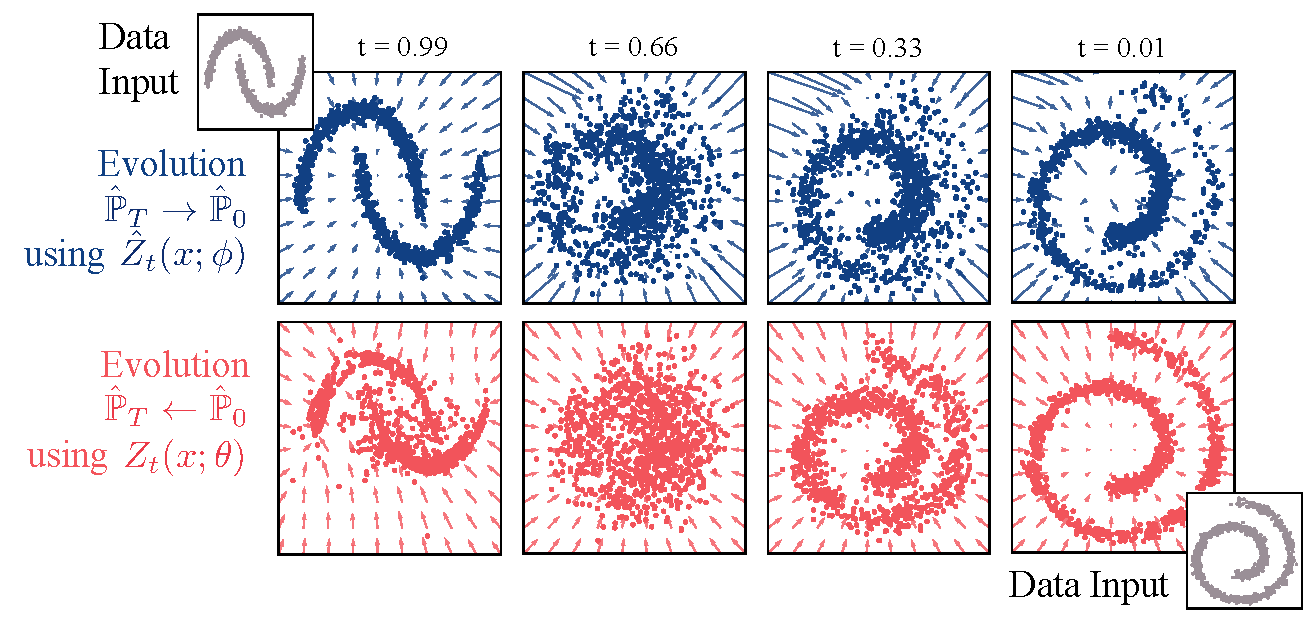
\includegraphics[width=0.8\linewidth]{figures/fig_pred_gsbve_toy_spiral_moon.pdf}
	\caption{Illustration of the time-dependent drifts learned by \textsc{GSBflow} with VE SDE for two toy marginal distributions. \emph{Top.} Evolution of $\distend$ (moons) $\rightarrow \distinit$ (spiral) via backward policy {\color{blue} $\SBb$}. \emph{Bottom.} Evolution of $\distinit$ (spiral) $\rightarrow \distend$ (moons) via forward policy {\color{pink} $\SBf$}.}
	\label{fig:res_synthetic}
\end{figure}

\begin{table}[ht]
    \caption{Evaluation of predictive performance w.r.t. the entropy-regularized Wasserstein distance $W_\varepsilon$ \citep{cuturi2013sinkhorn} of \textsc{GSBflow} and baselines on generating different \acrlong{sc} datasets (using 3 runs).}
    \label{tab:exp_wasserstein_cells}
    \centering
\adjustbox{max width=.7\linewidth}{%
    \begin{tabular}{lcc}
    \toprule
         \textbf{Method} & \multicolumn{2}{c}{\textbf{Tasks}} \\
         & \multicolumn{2}{c}{\makecell{Wasserstein Loss $W_\varepsilon \downarrow$}} \\
         \cmidrule{2-3}
         & \makecell{\citet{moon2019visualizing}} & \makecell{\citet{schiebinger2019optimal}}  \\
    \midrule
      \citet{song2020score} \\
        \tabindent \acrshort{VESDE} & $20.83 \pm 0.18$ & $40.81 \pm 0.42$ \\
        \tabindent sub-\acrshort{VPSDE} & $\mathbf{19.96 \pm 0.58}$ & $48.15 \pm 3.38$ \\
      \textsc{GSBflow} (\emph{ours}) \\
         \tabindent \acrshort{VESDE} & $25.18 \pm 0.10 $ & $\mathbf{27.85 \pm 0.68}$ \\
    \bottomrule
    \end{tabular}
}
\end{table}

\subsubsection{Synthetic Dynamics} 
\label{sec:gsbflow_synthetic}

Before conducting the \acrlong{sc} genomics experiments, we first test \textsc{GSBflow} on a synthetic setting. 
Our first task involves recovering the stochastic evolution of two-dimensional synthetic data containing two interleaving half circles ($\distend$) into a spiral ($\distinit$). 
\cref{fig:res_synthetic} shows the trajectories learned by \textsc{GSBflow} based on the \acrshort{VESDE} (see \cref{tab:examples}). 

While it is sufficient to parameterize only a single policy ({\color{blue} $\SBb$}) in generative modeling, the task of learning to evolve $\distinit$ into $\distend$ requires one to recover \emph{both} vector fields {\color{blue} $\SBb$} and {\color{pink} $\SBf$}.
As demonstrated in \cref{fig:res_synthetic}, \textsc{GSBflow} is able to successfully learn both policies {\color{pink} $\SBf$} and {\color{blue} $\SBb$} and reliably recovers the corresponding targets of the forward and backward evolution. While initializing the reference process through the closed-form \acrshort{SB} between the Gaussian approximations of both synthetic datasets provides good results, the power of \textsc{GSBflow} becomes evident in more complex applications which we tackle next.

\begin{figure}[t]
     \centering
	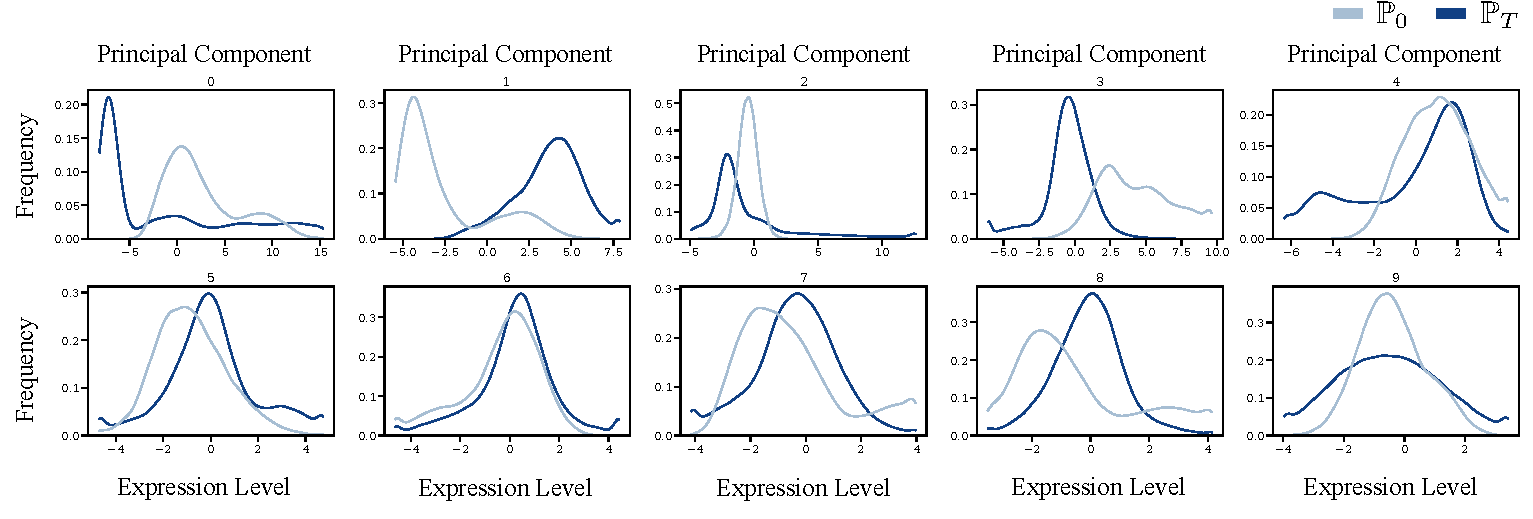
\includegraphics[width=\textwidth]{figures/fig_marginals_schiebinger_pcs_cropped.pdf}
 	\caption{The expression levels of the first 10 principal components from the dataset by \citet{schiebinger2019optimal}.}
	\label{fig:gaussianMain}
\end{figure}

\subsubsection{Single-Cell Dynamics}
\label{sec:gsbflow_cell}

% \looseness -1 Modern \acrlong{sc} profiling technologies are able to provide rich feature representations (e.g., gene expression) of \textit{individual} cells at any development stage. A crucial issue that arises with such profiling methods is their destructive nature: Measuring a cell requires destroying it and thus a cell cannot be measured twice. As a result, independent samples are collected at each snapshot, with no access to ground-truth \acrlong{sc} trajectories throughout time, resulting in challenging, \emph{unaligned}, datasets.
% Recovering cellular dynamics from such unaligned snapshots, i.e., $\distinit$ to $\distend$, has, however, extremely important scientific and biomedical relevance \citep{kulkarni2019beyond}. For example, it determines our understanding of how and why tumor cells evade cancer therapies \citep{frangieh2021multimodal} or unveils mechanisms of cell differentiation and development \citep{schiebinger2019optimal}. Following related work, in particular previous methods based on \acrlong{OT} \citep{schiebinger2019optimal, bunne2021learning, bunne2022supervised, tong2020trajectorynet}, the task is thus to learn the stochastic process that described the evolution of single cells from $\distinit$ to $\distend$.

Let us consider the evolution of \acrlong{sc} populations, for which we can collect the empirical distributions $\distinit,\distend$ of its expression levels at the times $t=0,1$ \citep{schiebinger2019optimal,moon2019visualizing}. 

\subsubsection*{Our choice of $\refsde$; the \textsc{GSBflow}.}

Instead of directly diving into the numerical solution of \acrshortpl{SB}, we first empirically verify that the distributions $\distinit,\distend$ in \acrlong{sc} genomics are typically close to \emph{non-standard} Gaussian distributions (see \cref{fig:gaussianMain} for the canonical dataset by \citet{schiebinger2019optimal}). 

Since the solutions of \acrshortpl{SB} are Lipschitz in terms of $\distinit,\distend$ \citep{carlier2022lipschitz}, a reasonable approximation to the original \acrshort{SB} objective is to replace $\distinit,\distend$ by Gaussians with matching moments. This results in a \acrshort{GSB} problem which can be solved in closed form by our \cref{thm:gaussian_sb}. Intuitively, if we denote an existing prior process by $\refsde$ and the solution of its corresponding \acrshort{GSB} by $\Xsol$, then $\Xsol$ presents a more appealing prior process than $\refsde$ since it carries the moment information of $\distinit$ and $\distend$, whereas $\refsde$ is completely data-oblivious.

Motivated by these observations, we propose a simple modification of the framework in \citet{chen2021likelihood}: Replace the prior process $\refsde$ by its \acrshort{GSB} approximation and keep everything else the same. The resulting scheme, which we term the \textsc{GSBflow}, learns a pair of forward {\color{pink} $\SBf$} and backward parametrized drifts {\color{blue} $\SBb$} that progressively transport samples from $\distinit \rightarrow \distend$ and $\distend \rightarrow \distinit$, respectively. The full algorithm is presented in \cref{alg:GSBflow} for completeness.

\subsubsection*{Single-cell genomics via \acrshortpl{GSB}.}

\begin{figure}[ht]
     \centering
     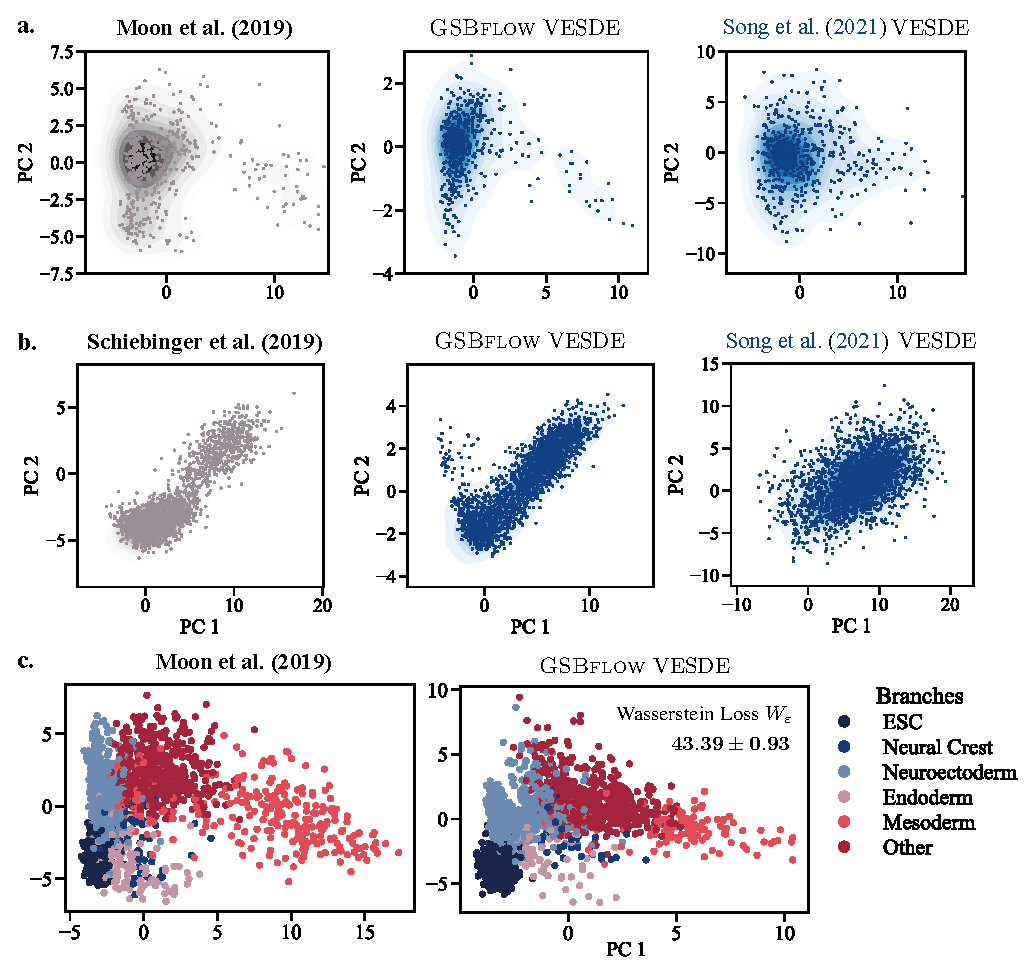
\includegraphics[width=\textwidth]{figures/fig_all_predictions.pdf}
    \caption{\textbf{a.}-\textbf{b.} Visual evaluation of the ability of our method to model the \textbf{generation} of data from \textbf{a.} \citet{moon2019visualizing} and \textbf{b.} \citet{schiebinger2019optimal}. Density plots are visualized in 2D \acrshort{PCA} space and show generated data points using either \textsc{GSBflow} (our method) or the procedure in \citet{song2020score}. \textbf{c.} Evaluation of \textsc{GSBflow}'s ability to model the entire \textbf{evolution} of a developmental process of \citet{moon2019visualizing}, visualized by the data and \textsc{GSBflow} predictions colored by the lineage branch class.}
    \label{fig:all_results}
\end{figure}

\paragraph{Generative modeling setting.}
\looseness -1 We investigate the ability of \textsc{GSBflow} to generate cell populations $\distend$ from noise $\Ncal_0$ ($\Ncal_0 \rightarrow \distend$, \cref{fig:all_results}a, b) on the canonical datasets \citep{moon2019visualizing, schiebinger2019optimal}; as well as to predict the dynamics of \acrlong{sc} genomics ($\distinit \rightarrow \distend$, \cref{fig:all_results}c) \citep{moon2019visualizing}, i.e., the inference of cell populations $\distend$ resulting from the developmental process of an initial cell population $\distinit$, with the goal of learning individual dynamics, identify ancestor and descendant cells. 
% In addition, in order to test our hypothesis that the moment information carried by \textsc{GSBflow} leads to better overall performance, we scale the datasets \citep{moon2019visualizing, schiebinger2019optimal} by 20 and repeat each training procedure.
% We consider the development of human \acrshortpl{ESC} grown as \acrlongpl{EB} into diverse cell lineages monitored by \acrshort{sc}\acrshort{RNAseq} methods \citep{moon2019visualizing} as well as reprogramming \acrshortpl{MEF} into \acrshortpl{iPSC} \citep{schiebinger2019optimal}.
The evaluation is conducted on the first 20 or 30 components of the \acrshort{PCA} space of the >~1500 highly differentiable genes.

\looseness -1 We evaluate the quality of the generated cellular states through the entropy-regularized Wasserstein distance $W_\varepsilon$
(see \cref{tab:exp_wasserstein_cells}) and by visualizing the first two principal components (PC), see \cref{fig:all_results}a,~b.
\textsc{GSBflow} performs competitively on reconstructing \acrshort{EB} differentiation landscapes \citep{moon2019visualizing}, and outperforms \acrlongpl{SGM} baselines on the \acrlong{iPSC} reprogramming task \citep{schiebinger2019optimal} as quantified by $W_\varepsilon$ between data and predictions.
For more details on datasets and evaluation metrics, see \cref{app:datasets} and \cref{app:evaluation_metrics}, respectively.

\paragraph{Interpolation setting.}
Further, we analyze \textsc{GSBflow}'s ability to predict the temporal evolution of \acrshort{EB} differentiation \citep{moon2019visualizing}, where cells measured at day 1 to 3 serve as samples of $\distinit$, while $\distend$ is constructed from samples between day 12 to 27. As no ground truth trajectories are available in the data, we compare the predicted evolution to the data and compare how well the heterogeneity of lineage (\cref{fig:all_results}c, upper panel) is captured.
\cref{fig:all_results}c (lower panel) closely resembles the data (see $W_\varepsilon$ in \cref{fig:all_results}c) and thus demonstrate \textsc{GSBflow}'s ability to learn cell differentiation into various lineages and to capture biological heterogeneity on a more macroscopic level.

\subsection{Discussion}
\looseness -1 We derive closed-form solutions of \acrshortpl{GSB}, an important class of dynamic \acrshort{OT} problems. Our technique originates from a deep connection between Gaussian \acrshort{OT} and the Bures-Wasserstein geometry, which we generalize to the case of general \acrshort{SB} problems. Numerically, we demonstrate that our new closed forms inspire a simple modification of existing \acrshort{SB}-based numerical schemes, which can however lead to significantly improved performance.

\paragraph{Limitations of our framework.}
\looseness -1 In a broader context, we hope our results can serve as the inspiration for more learning algorithms, much like how existing closed-form solutions of Gaussian \acrshort{OT} problems have contributed to the machine learning community. We thus acknowledge a severe limitation of our closed-form solutions: These formulas require matrix inversions, which might face scalability issues for high-dimensional data. In addition, existing matrix inversion algorithms are typically extremely sensitive to the condition number, and thus our formulas are not as useful for ill-conditioned data. Lifting these constraints to facilitate further applications, such as to image datasets, is an important future work.

\newpage
\section{Diffusion Schr{\"o}dinger Bridges from Sparse Trajectories}
\label{sec:sbalign}

\begin{figure}[H]
    \centering
    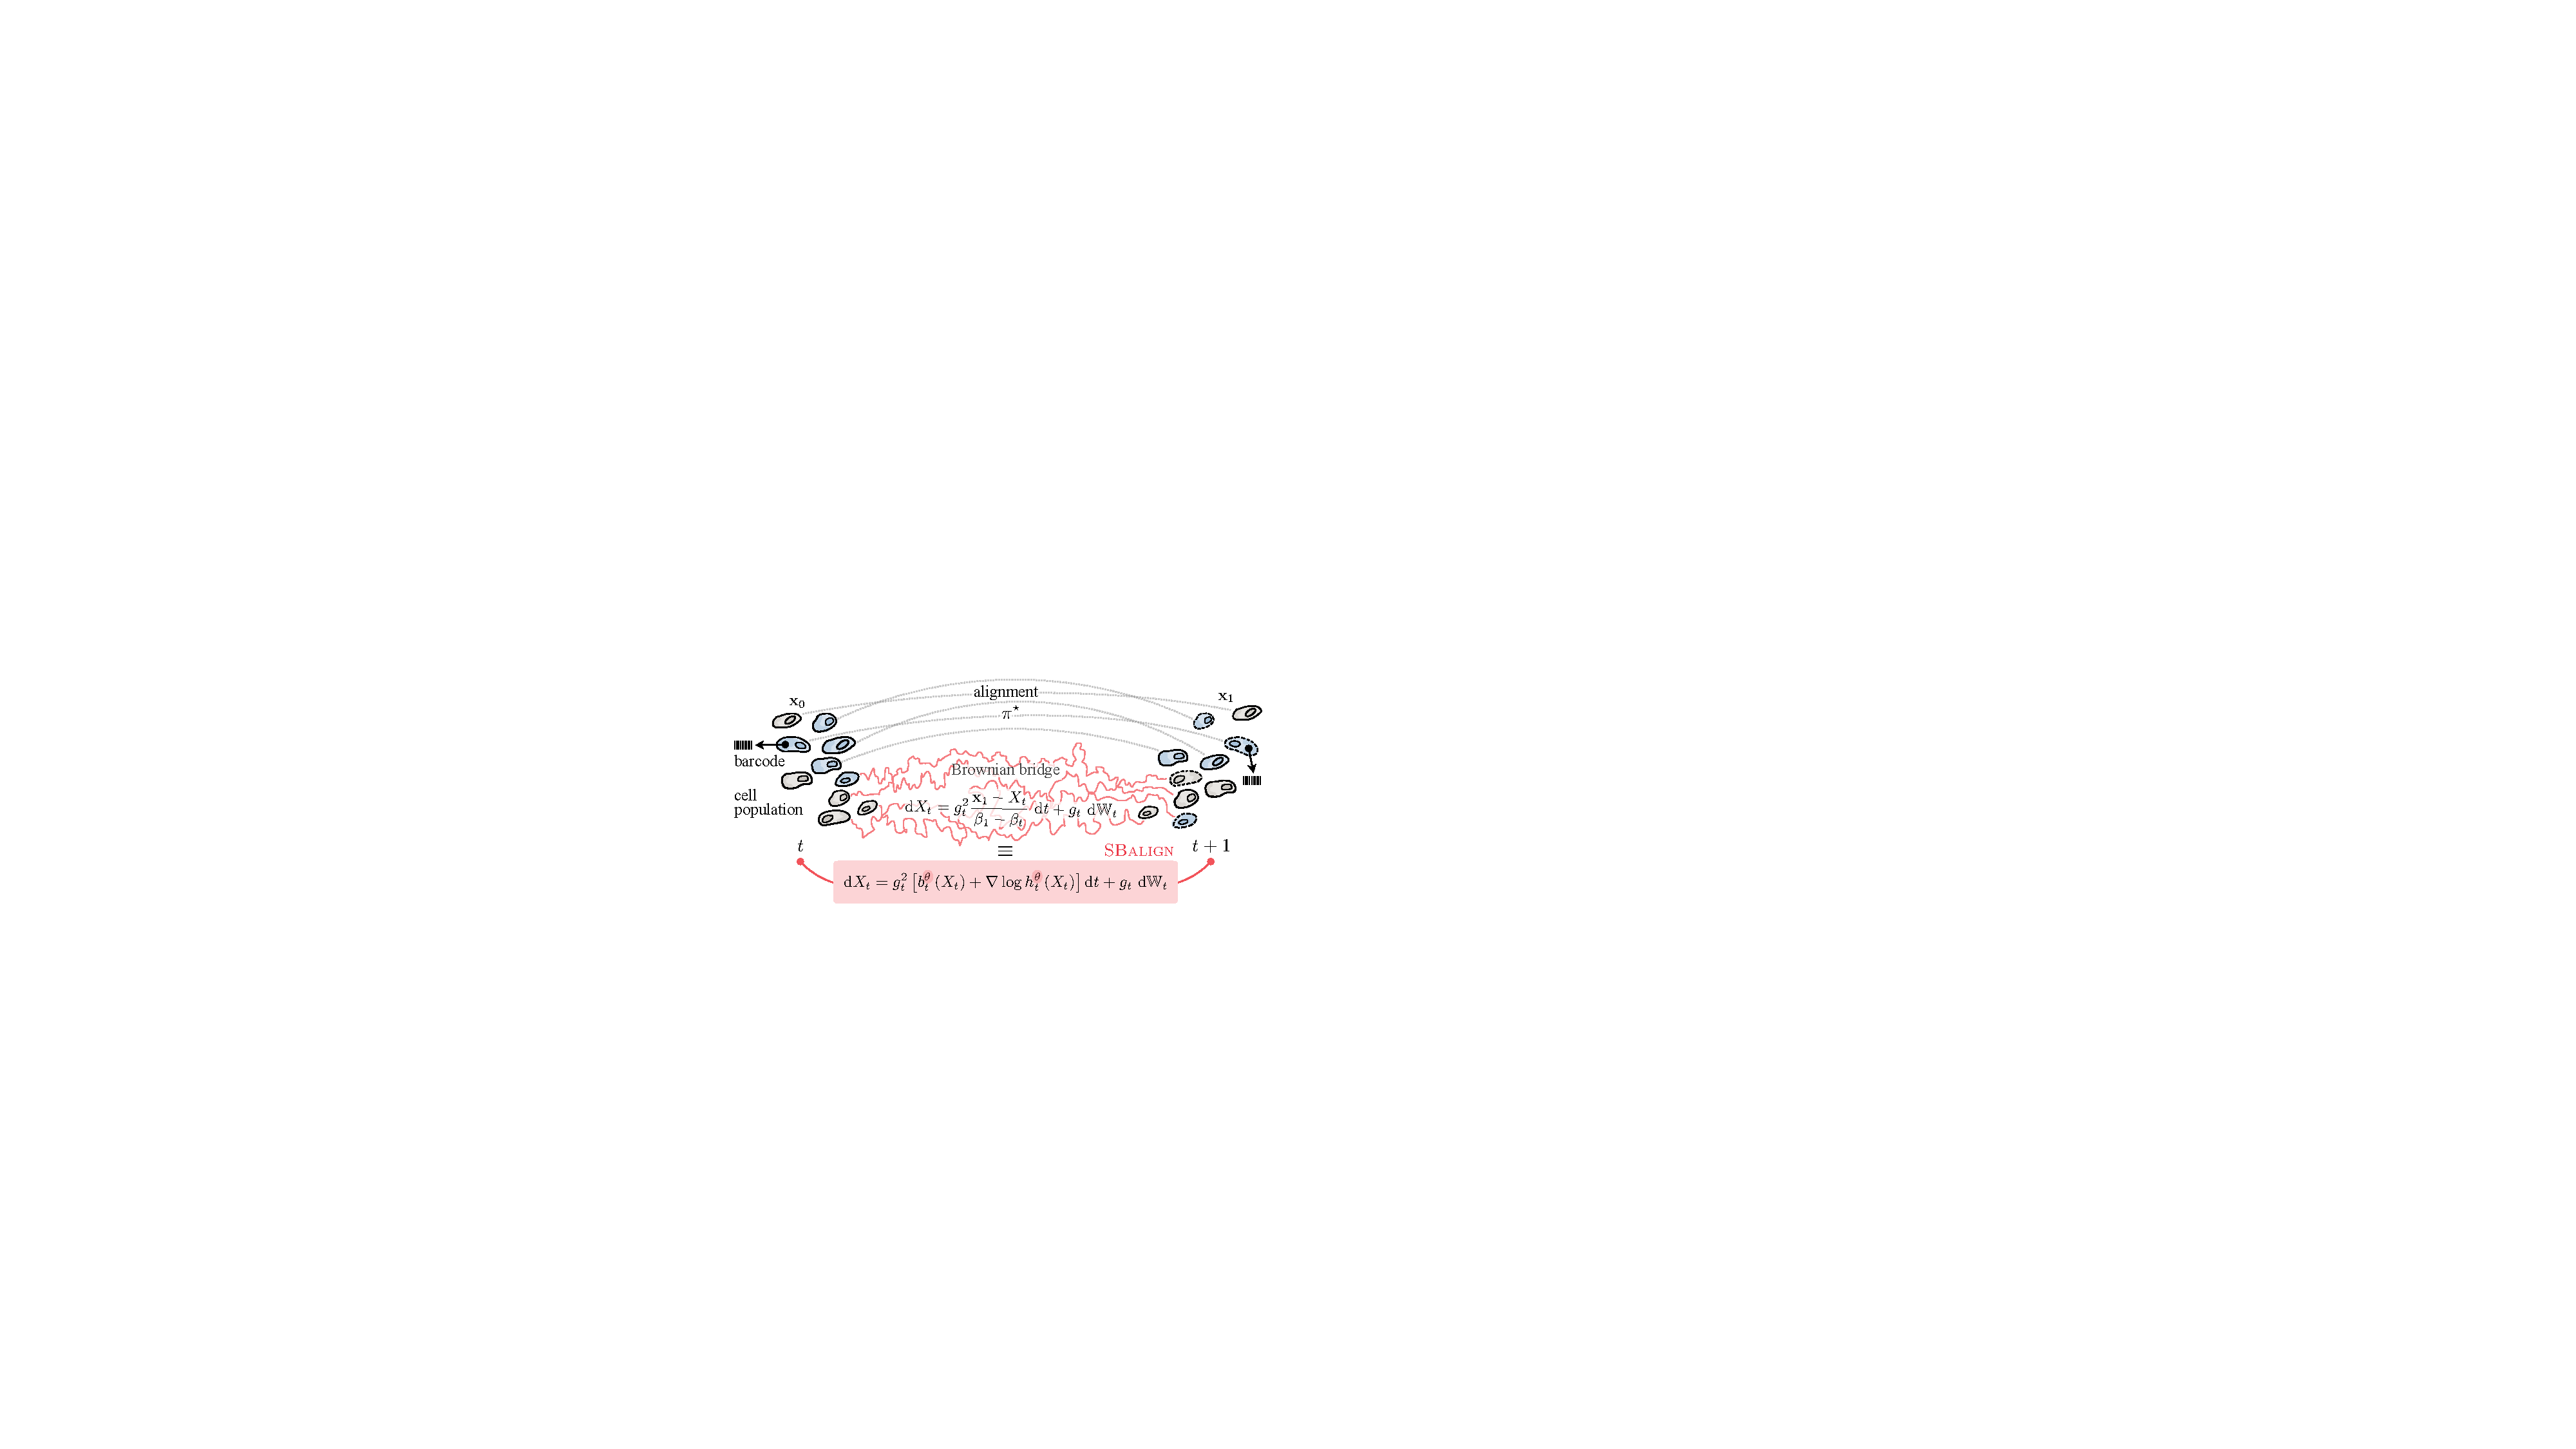
\includegraphics[width=.8\linewidth]{figures/fig_overview_sbalign.pdf}
    \caption{\textbf{Overview of \textsc{SBalign}.} In the setting of cell differentiation we aim at learning the evolutionary process that morphs a population from its stat at $t$ to $t+1$. Through genetic tagging (i.e., barcodes) we are able to trace progenitor cells at time point $t$ into their descendants $t+1$. This provides us with an alignment between populations at consecutive time steps. Our goal is then to recover a stochastic trajectory from $\x_0$ to $\x_1$. To achieve this, we connect the characterization of an SDE conditioned on $\x_0$ and $\x_1$ (utilizing the Doob's \emph{$h$-transform}) with that of a Brownian bridge between $\x_0$ and $\x_1$ (classical Schr{\"o}dinger bridge theory), leading to a simpler training procedure with lower variance and strong empirical results.}
    \label{fig:overview_sbalign}
\end{figure}

As introduced in the previous chapter, \acrlongpl{DSB} \citep{de2021diffusion,chen2021likelihood,vargas2021solving,liu2022deep} have recently emerged as a powerful paradigm due to their ability to generalize prior deep diffusion-based models, notably \acrlong{SMLD}
\citep{song2019generative,song2020score} and \acrlongpl{DDPM} \citep{ho2020denoising}, which have achieved the state-of-the-art on many generative modeling problems.
Despite the wide success, a significant limitation of existing frameworks for solving \acrshortpl{DSB} is that they fail to capture the \emph{alignment} of data: If $\distinit, \distend$ are two (empirical) distributions between which we wish to interpolate, then a tacit assumption in the literature is that the dependence of $\distinit$ and $\distend$ is unknown and somehow has to be recovered. Such an assumption, however, ignores important scenarios where the data is \emph{aligned}, meaning that the samples from $\distinit$ and $\distend$ naturally come in pairs $(\x^i_0,\x^i_1)_i^{N}$, which is common in many biological phenomena. 
% Proteins, for instance, undergo conformational changes upon interactions with other biomolecules (protein docking). The goal is to model conformational changes by recovering a (stochastic) trajectory $\x_t$ based on the positions observed at two-time points $\left(\x_0, \x_1\right)$. Failing to incorporate this alignment would mean that we completely ignore information on the correspondence between the initial and final points of the molecules, resulting in a much harder problem than necessary.
Cells change their molecular profile throughout developmental processes \citep{schiebinger2019optimal,bunne2022proximal} or in response to perturbations such as cancer drugs \citep{lotfollahi2019scgen,bunne2021learning}. As most measurement technologies are destructive assays, i.e., the same cell cannot be observed twice nor fully profiled over time, these methods aim at reconstructing cell dynamics from \emph{unpaired} snapshots.
Recent developments in molecular biology, however, aim at overcoming this technological limitation. For example, \citet{chen2022live} propose a transcriptome profiling approach that preserves cell viability. \citet{weinreb2020lineage} capture cell differentiation processes by clonally connecting cells and their progenitors through barcodes (see \cref{fig:overview_sbalign}).

Motivated by these observations, the goal of this section is to propose a novel algorithmic framework for solving \acrshortpl{DSB} with (partially) \emph{aligned} data. Our approach is in stark contrast to existing works which, due to the lack of data alignment, all rely on some variants of \acrshort{IPF} \citep{fortet1940resolution, kullback1968probability} and are thus prone to numerical instability. On the other hand, via a combination of the original theory of Schr{\"o}dinger bridges \citep{schrodinger1931umkehrung,leonard2013survey} and the key notion of Doob's \emph{$h$-transform} \citep{doob1984classical, rogers2000diffusions}, we design a novel loss function that completely bypasses the \acrshort{IPF} procedure and can be trained with much lower variance. \\


To summarize, we make the following contributions:
\begin{itemize}[topsep=0pt]
\item To our best knowledge, we consider, for the first time, the problem of interpolation with \emph{aligned} data. We rigorously formulate the problem in the \acrshort{DSB} framework.

\item Based on the theory of Schr{\"o}dinger bridges and $h$-transform, we derive a new loss function that, unlike prior work on \acrshortpl{DSB}, does not require an \acrshort{IPF}-like procedure to train. We also propose principled regularization schemes to further stabilize training.

\item We describe how interpolating aligned data can provide better reference processes for use in classical \acrshortpl{DSB}, paving the way to hybrid aligned/non-aligned \acrshortpl{SB}.

\item \looseness -1 We evaluate our proposed framework on both synthetic and real data. For experiments utilizing real data based on barcoded measurements of cell differentiation in hematopoiesis.
Our method demonstrates a considerable improvement over prior methods across various metrics, thereby substantiating the importance of taking the data alignment into account. 
\end{itemize}

\paragraph{Related work.}

Solving \acrshortpl{DSB} is a subject of significant interest in recent years and has flourished in a number of different algorithms \citep{de2021diffusion,chen2021likelihood,vargas2021solving,bunne2022recovering,liu2022deep}. However, all these previous approaches focus on  \emph{unaligned} data, and therefore the methodologies all rely on \acrshort{IPF} and are hence drastically different from ours. In the experiments, we will demonstrate the importance of taking the alignment of data into consideration by comparing our method to these baselines.

An important ingredient in our theory is Doob's $h$-transform, which has recently also been utilized by \citet{liu2023learning} to solve the problem of constrained diffusion. However, their fundamental motivation is different from ours. \citet{liu2023learning} focus on learning the drift of the diffusion model and the $h$-transform \emph{together}, whereas ours is to read off the drift \emph{from} the $h$-transform with the help of {\em aligned data}. Consequently, there is no overlap between the two algorithms and their intended applications. 

To the best of our knowledge, the concurrent work of \citet{tong2023conditional} is the only existing framework that can tackle aligned data, which, however, is not their original motivation. In the context of solving \acrshortpl{DSB}, their algorithm can be seen as learning a vector field that generates the correct \emph{marginal} probability \citep[cf.][Proposition 4.3]{tong2023conditional}. Importantly, this is different from our aim of finding the \emph{pathwise} optimal solution of \acrshortpl{DSB}: If $(\x^i_{0,\textup{test}})_{i=1}^m$ is a test data set for which we wish to predict their destinations, then the framework of \citet{tong2023conditional} can only ensure that the marginal distribution $(\x^i_{1,\textup{test}})_{i=1}^m$ is correct, whereas ours is capable of predicting that $\x^i_{1,\textup{test}}$ is precisely the destination of $\x^i_{0,\textup{test}}$ for each $i$. 

\paragraph{Problem formulation.}

Suppose that we are given access to i.i.d. \emph{aligned} data $(\x_0^i,\x_1^i)_{i=1}^N$, where the marginal distribution of $\x^i_0$'s is $\distinit$ and of $\x_1^i$'s is $\distend$. Typically, we view $\distinit$ as the empirical marginal distribution of a stochastic process observed at time $t= 0$, and likewise $\distend$ the empirical marginal observed at $t=\horizon$. The goal is to reconstruct the stochastic process $\Pmargin$ based on $(\x_0^i,\x_1^i)_{i=1}^N$, i.e., to \emph{interpolate} between $\distinit$ and $\distend$.

Such a task is ubiquitous in biological applications. Besides cell trajectories of dynamical processes in tissues, a prominent application concerns molecular dynamics simulations. Here, we have access to trajectories $\left(\x_t^i\right)_{t \in [0, 1]}$, where $\x_0^i$ and $\x_1^i$ represent the initial and final positions of the $i$-th molecule respectively. Any learning algorithm using these simulations should be able to respect the provided alignment. 

\subsection{\textsc{SBalign}: Aligned Diffusion Schr{\"o}dinger Bridges}

In this section, we derive a novel loss function for \acrshortpl{DSB} with aligned data by combining two classical notions: The theory of \acrlongpl{SB} \citep{schrodinger1931umkehrung,leonard2013survey,chen2021stochastic} and Doob's $h$-transform \citep{doob1984classical, rogers2000diffusions}. We then describe how solutions to DSBs with aligned data can be leveraged in the context of classical \acrshortpl{DSB}.

\paragraph{Static SB and aligned data.}

Our starting point is the simple and classical observation that the dynamic \acrlong{SB} problem \eqref{eq:schrodinger_bridge} is the continuous-time analog of the \emph{entropic optimal transport}, also known as the \emph{static} \acrlong{SB} problem \citep{leonard2013survey,chen2021stochastic,peyre2019computational}
\begin{equation}
\label{eq:static-SB}
\Pssol \defeq \argmin_{ \substack{ \Pinit = \distinit, \; \Pend = \distend} } \KL( \mathbb{P}_{0,1} \| \refprobase_{0,1}),
\end{equation}
where the minimization is over all \emph{couplings} of $\distinit$ and $\distend$, and $\refprobase_{0,1}$ is simply the joint distribution of $\refpro$ at $t=0,\horizon$. In other words, if we denote by $\Psol$ the stochastic process that minimizes \eqref{eq:SB}, then the joint distribution $\Psol[0,\horizon]$ necessarily coincides with the $\Pssol$ in \eqref{eq:static-SB}. Moreover, since in \acrshortpl{DSB} the data is always assumed to arise from $\Psol$, we see that:
\begin{quote}
The \emph{aligned} data $(\x_0^i,\x_1^i)_{i=1}^N$ constitutes samples of $\Pssol$.
\end{quote}
This simple but crucial observation lies at the heart of all derivations to come. 

Our central idea is to represent $\Psol$ via two different, but equivalent, characterizations, both of which involve $\Pssol$: That of a \emph{mixture} of reference processes with pinned endpoints, and that of conditional \acrlongpl{SDE}.

\paragraph{$\Psol$ from $\Pssol$: $\refpro$ with pinned end points.}

For illustration purposes, from now on, we will assume that the reference process $\refpro$ is a Brownian motion with diffusion coefficient $\volat$:
% \footnote{\looseness -1 Extension to more involved reference processes is conceptually straightforward but notationally clumsy. Furthermore, reference processes of the form \eqref{eq:gtWt} are dominant in practical applications \citep{song2020score, bunne2022recovering}, so we omit the general case. }
\begin{equation}
\label{eq:gtWt}
\dd \refpro = \volat \mathrm{d}\gW_t.
\end{equation}
In this case, it is well-known that $\refpro$ \emph{conditioned} to start at $\x_0$ and end at $\x_1$ can be written in another \acrshort{SDE} \citep{mansuy2008aspects, liu2023learning}:
\begin{equation}
\label{eq:BB}
\dd X_t = \volatsq[\ctime] \frac{\x_1-X_t}{\cvolat[\horizon]-\cvolat[\ctime]} \dt + \volat\mathrm{d}\gW_t
\end{equation}
where $X_0 = \x_0$ and %, $\dWiener$ is itself a Brownian motion, and 
\begin{equation}
\cvolat\defeq \int_0^\ctime \volatsq \dd s.
\end{equation}We call the processes in \eqref{eq:BB} the \emph{scaled Brownian bridges} as they generalize the classical Brownian bridge, which corresponds to the case of $\volat \equiv 1$.

The first characterization of $\Psol$ is then an immediate consequence of the following classical result in \acrlong{SB} theory: Draw a sample $(\x_0, \x_1) \sim \Pssol$ and connect them via \eqref{eq:BB}. The resulting path is a sample from $\Psol$ \citep{leonard2013survey, chen2021stochastic}. In other words, $\Psol$ is a \emph{mixture} of scaled Brownian bridges, with the mixing weight given by $\Pssol$.

\paragraph{$\Psol$ from $\Pssol$: SDE representation.}

Another characterization of $\Psol$ is that it is itself given by an \acrshort{SDE} of the form \citep{leonard2013survey, chen2021stochastic}
\begin{equation}
\label{eq:SB-SDE}
\dd X_t = \volatsq[\ctime]\fdrift(X_t) \dt + \volat\mathrm{d}\gW_t.
\end{equation}
Here, $\fdrift: \R^d \to \R^d$ is a time-dependent drift function that we wish to learn.

Now, by Doob's h-transform, we know that the \acrshort{SDE} \eqref{eq:SB-SDE} \emph{conditioned} to start at $\x_0$ and end at $\x_1$ is given by another \acrshort{SDE}  \citep{doob1984classical,rogers2000diffusions}:
\begin{equation}
\label{eq:SB-SD-conditioned}
\dd X_t = \volatsq[\ctime]\bracks*{\fdrift(X_t) + \nabla \log \doob(X_t) }\dt +\volat \mathrm{d}\gW_t
\end{equation}
where $\doob(\x) \defeq \prob(X_1 = \x_1\vert X_t = \x)$ is the \emph{Doob's $h$ function}. Notice that we have suppressed the dependence of $\doob$ on $\x_0$ and $\x_1$ for notational simplicity. % \footnote{The fact $\doob$ does not depend on the starting point $\x_0$ is easily understood: An \acrshort{SDE} remains the same no matter where it starts.}

\paragraph{Loss function.}

Since both \eqref{eq:BB} and \eqref{eq:SB-SD-conditioned} represent $\Psol$, the solution of the \acrshortpl{DSB}, the two \acrshortpl{SDE} must coincide. 
% This in turn implies that, for all $(\x_0,\x_1)\sim\Pssol$, we must have
% \begin{equation}
% \fdrift(X_t) + \nabla \log \doob(X_t) =  \frac{\x_1-X_t}{\cvolat[\horizon]-\cvolat[\ctime]}.
% \end{equation}
In other words, suppose we parametrize $\fdrift$ as $\fdrift^\theta$, then, by matching terms in \eqref{eq:BB} and \eqref{eq:SB-SD-conditioned}, we can learn the optimal parameter $\theta^\star$ via optimization of the loss function
\begin{equation}
\label{eq:loss}
\Loss(\theta) \defeq \exof*{\int_0^1 \norm*{ \frac{\x_1-X_t}{\cvolat[\horizon]-\cvolat[\ctime]}-\nabla \log \doob^\theta(X_t)}^2 \dt  }
\end{equation}where $\doob^\theta$ is determined by $\fdrift^\theta$ as well as the drawn samples $(\x_0,\x_1)$. In short, assuming that, for each $\theta$, we can compute $\doob^\theta$ \emph{based only on} $\fdrift^\theta$, we can then backpropagate through \eqref{eq:loss} and optimize it using any off-the-shelf algorithm.

\paragraph{A slightly modified \eqref{eq:loss}.}
Even with infinite data and a neural network with sufficient capacity, the loss function defined in \eqref{eq:loss} does converge to 0. For the purpose of numerical stability, we instead propose to modify \eqref{eq:loss} to:
\begin{equation}
\label{eq:loss_modified}
\Loss(\theta) \defeq \exof*{\int_0^1 \norm*{\frac{\x_1-X_t}{\cvolat[\horizon]-\cvolat[\ctime]}- \left(\fdrift^\theta + \nabla \log \doob^\theta(X_t)\right)}^2 \dt  }
\end{equation}which is clearly equivalent to \eqref{eq:loss} at the true solution of $\fdrift$. Notice that \eqref{eq:loss_modified} bears a similar form as the popular score-matching objective employed in previous works \citep{song2019generative,song2020score}:
\begin{equation}
\label{eq:score_matching}
\Loss(\theta) \defeq \exof*{\int_0^1 \norm*{\nabla \log p(\x_t | \x_0)- s^\theta(X_t, t)}^2 \dt  },
\end{equation}
where the term $\frac{\x_1-X_t}{\cvolat[\horizon]-\cvolat[\ctime]}$ is akin to $\nabla \log p(\x_t | \x_0)$, while $\left(\fdrift^\theta + \nabla \log \doob^\theta(X_t)\right)$ corresponds to $s^\theta(X_t, t)$. 

 \begin{algorithm}[t]
   \caption{\textsc{SBalign}}
   \label{alg:SBalign}
\begin{algorithmic}
   \STATE {\bfseries Input:} Aligned data $(\x^i_0,\x^i_1)_{i=1}^N$, learning rates $\lrf,\lrb$, training iterations $K$. % \dots  data $x_i$, size $m$
   \STATE {\bfseries Output:} Optimal drift $\fdrift^\theta$ and parameterization $m^{\phi}$ of the "softened" Doob's $h$-transform $\doobs$
%  \STATE {\bfseries Construct \eqref{eq:GaussianSB}:} Compute the means and covariances of $\distinit, \distend$.
%  \REPEAT
\smallskip
   \STATE Initialize $\paramf \subs \paramf_0$, $\paramb \subs \paramb_0$
   \FOR{$k=1$ {\bfseries to} $K$} 
   \STATE Draw a mini-batch of samples from $(\x^i_0,\x^i_1)_{i=1}^N$
%  \FOR{$j=1$ {\bfseries to} $\inneriter$}   
%  \IF{$j \mod \caching = 0$}
   \STATE Compute empirical average of loss $\Loss$ \eqref{eq:loss_final} with mini-batch
%  \ENDIF
%  \STATE Compute $\lossb$ via \eqref{eq:loss-backward}
   \STATE Update $\paramb \subs \paramb - \lrb\nabla \Loss(\theta,\phi)$
%  \ENDFOR
%  \FOR{$j=1$ {\bfseries to} $\inneriter$}   
%  \IF{$j \mod \caching = 0$}
%  \STATE Simulate \eqref{eq:GSB-sde-backward} with $\point_\horizon \sim \distend$
%  \ENDIF
%  \STATE Compute $\lossf$ via \eqref{eq:loss-forward}
   \STATE Update $\paramf \subs \paramf - \lrf\nabla \Loss(\theta,\phi)$
   \ENDFOR
%  \ENDFOR
%  \UNTIL{$noChange$ is $true$}
\end{algorithmic}
\end{algorithm}

\paragraph{Computing $\doob^\theta$.}

Inspecting $\doob$ in \eqref{eq:SB-SD-conditioned}, we see that, given $(\x_0,\x_1)$, it can be written as the conditional expectation of an indicator function:
\begin{equation}
\label{eq:h-semigroup}
\doob(\x) = \prob(X_1 = \x_1\vert X_t = \x) = \exof*{
\one_{\{\x_1\}}\vert X_t = \x}
\end{equation}where the expectation is over \eqref{eq:SB-SDE}. Functions of the form \eqref{eq:h-semigroup} lend themselves well to computation since it solves simulating the \emph{unconditioned} paths.
% since the Feymann-Kac formula, which offers a representation via simulating the \emph{unconditional} paths. 
Furthermore, in order to avoid overfitting on the given samples, it is customary to replace the "hard" constraint $\one_{\{\x_1\}}$ by its \emph{smoothed} version \citep{zhang2021path, holdijk2022path}: 
\begin{equation}
\label{eq:softdoob}
\doobs(\x) \defeq \exof*{  \exp\parens*{-\frac{1}{2\reg}\norm{X_\horizon-\x_1}^2 }  \vert X_t = \x}.
\end{equation}
Here, $\reg$ is a regularization parameter that controls how much we ``soften'' the constraint, and we have $\lim_{\reg\to 0} \doobs = \doob$.

Although the computation of \eqref{eq:softdoob} can be done via a standard application of the Feynman-Kac formula \citep{rogers2000diffusions}, an altogether easier approach is to parametrize $\doobs$ by a second neural network $m^{\phi}$ and perform alternating minimization steps on $\fdrift^\theta$ and $m^{\phi}$. This way, we can also avoid simulating even the unconditional paths of \eqref{eq:SB-SDE}, thereby further reducing the variance in training.

\begin{figure*}[t]
    \centering
    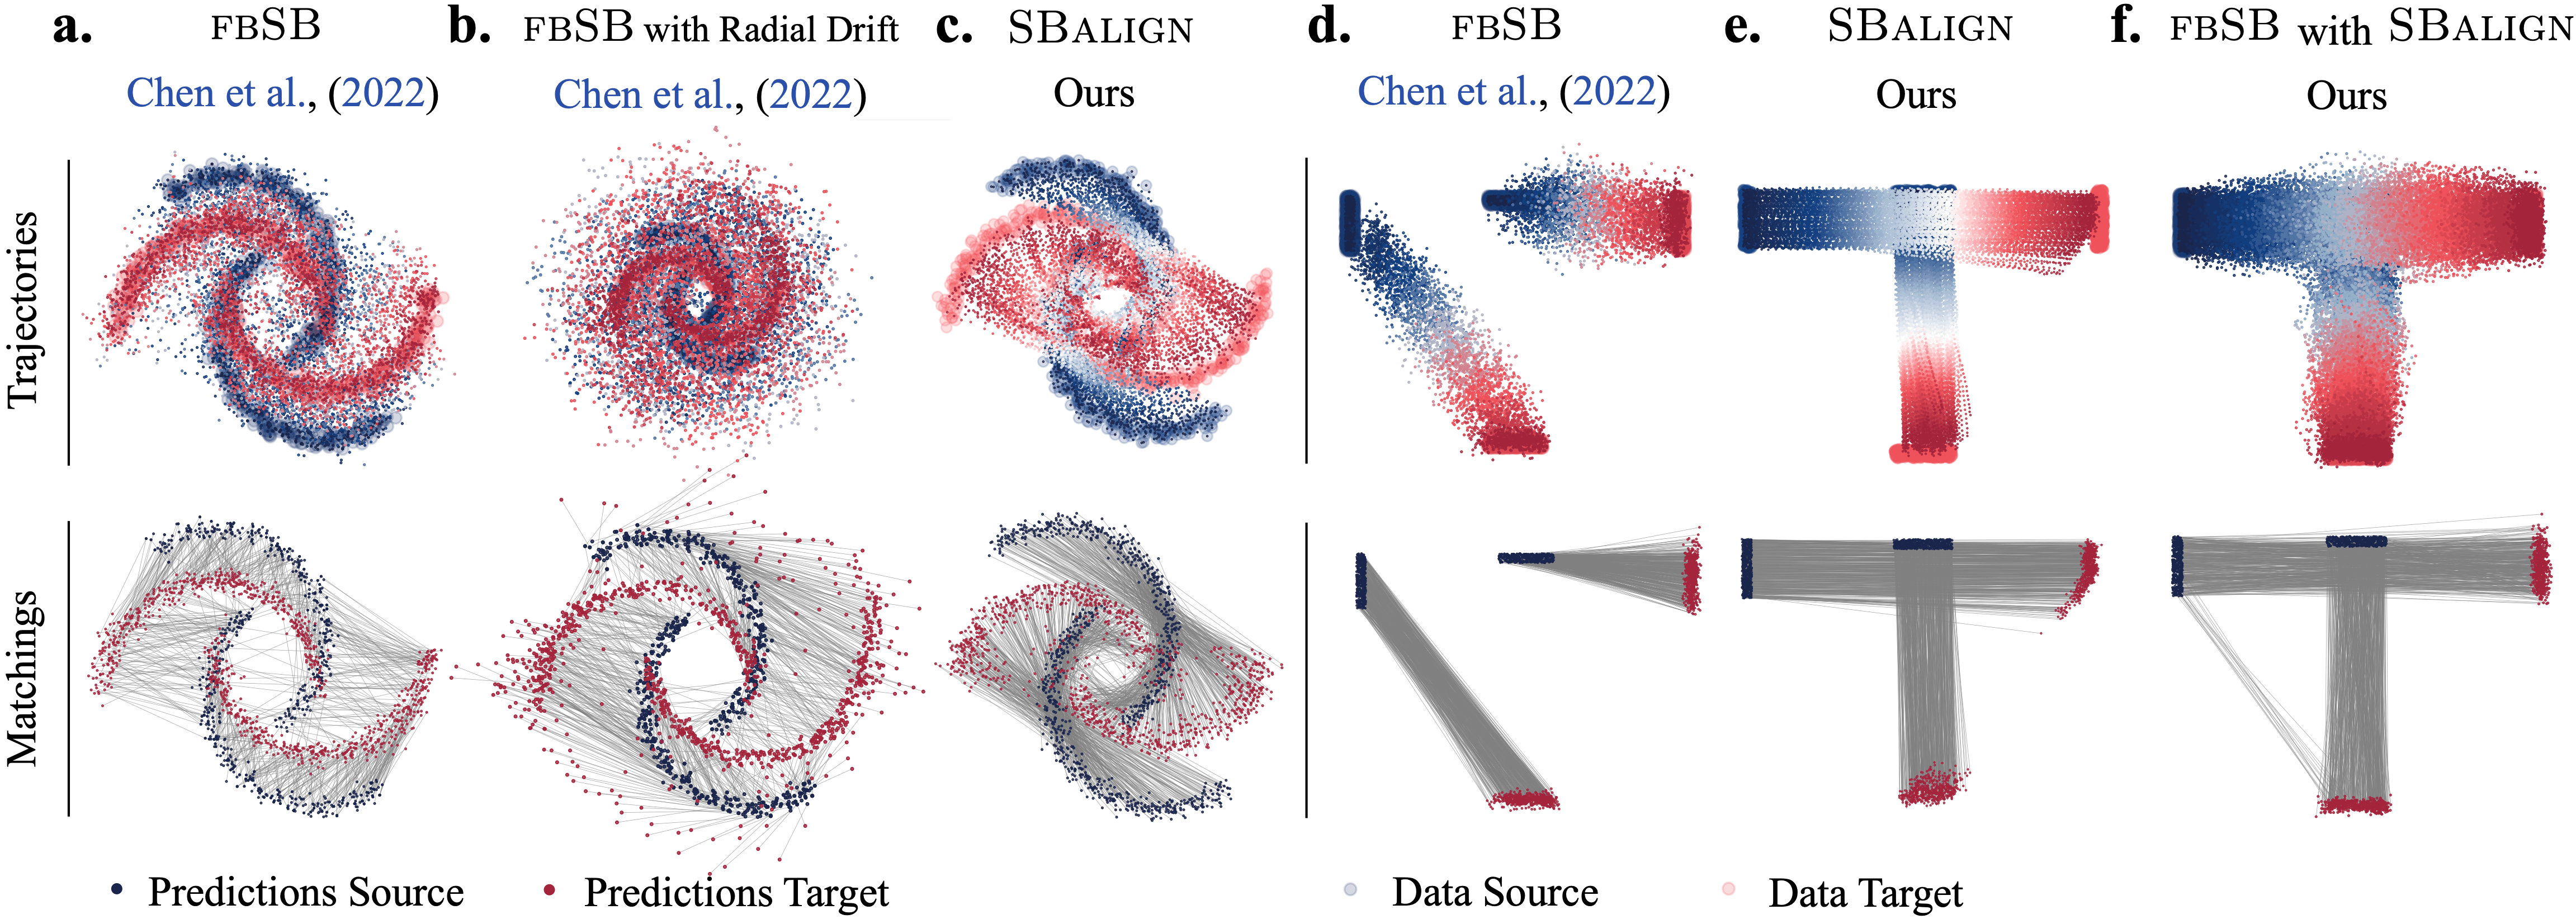
\includegraphics[width=\textwidth]{figures/fig_results_synthetic.png}
    \caption{Experimental results on the Moon dataset (\textbf{a-c}) and T-dataset (\textbf{d-f}). The top row shows the trajectory sampled using the learned drift, and the bottom row shows the matching based on the learned drift. Compared to other baselines, \textsc{SBalign} is able to learn an appropriate drift respecting the true alignment. (\textbf{f}) further showcases the utility of \textsc{SBalign}'s learned drift as a suitable reference process to improve other training methods.}
    \label{fig:results_spiral}
\end{figure*}

\paragraph{Regularization.}
Since it is well-known that $\nabla \log\doob$ typically explodes when $\ctime\to 1$ \citep{liu2023learning}, it is important to regularize the behavior of $m^{\phi}$ for numerical stability, especially when $\ctime\to 1$. Moreover, in practice, it is desirable to learn a drift $\fdrift^\theta$ that respects the data alignment \emph{in expectation}: If $(\x_0,\x_1)$ is an input pair, then multiple runs of the \acrshort{SDE} \eqref{eq:SB-SDE} starting from $\x_0$ should, on average, produce samples that are in the proximity of $\x_1$. This observation implies that we should search for drifts whose corresponding $h$-transforms are diminishing.

A simple way to simultaneously achieve the above two requirements is to add an $\ell^2$-regularization term, resulting in the loss function:
% \eqref{eq:logdoobs} is computationally expensive to simulate, because of repeated function calls to $\fdrift^\theta$, and also suffers from high variance, especially in the initial stages of training. 
% Note $\nabla \log \doobs(\x_1) = 0$. We replace $\nabla \log \doobs(\x)$ with a neural network $m^{\phi}$ such that $\norm{m^{\phi}(\x_1)}$ is minimized. The final loss function looks like
\begin{align}
\label{eq:loss_final}
\Loss(\theta,\phi) &\defeq \mathbb{E} \Bigg[\int_0^1 \norm*{\frac{\x_1-X_t}{\cvolat[\horizon]-\cvolat[\ctime]}- \left(\fdrift^\theta + m^{\phi}(X_t)\right)}^2
\\ &\hspace{35mm}+ \lambda_t \norm{m^{\phi}(\x_t)}^2 \dt \Bigg]
\nonumber
\end{align}where $\lambda_t$ can either be constant or vary with time. The overall algorithm is depicted in \cref{alg:SBalign}.


\subsection{Aligned Schr\"odinger Bridges as Prior Processes}
\label{subsec:prior_drift}

% Classical SBs are unsuitable in cases where the alignments are known because they only consider samples from $\distinit$ and $\distend$ and disregard those drawn from the (optimal) coupling $\pi^\star$. However, the reliance of our method on this crucial knowledge is critical to avoid the necessity of IPF-like iterates but may become a limitation when insufficient information on alignments is available. 

% In such a situation, while it is unrealistic to hope for an accurate solution to the aligned SB problem, the interpolation between $\distinit$ and $\distend$ learned by \textsc{SBalign} (\ref{eq:SB-SDE}) can potentially still be leveraged to obtain a better reference process, when solving a classical SB on the same marginals ---i.e. the term $b_t(X_t)$ learned via \textsc{SBalign} can, in fact, be used \textit{as is} to construct a data-informed alternative $\Tilde{\refpro}$ to the standard Brownian motion (\ref{eq:gtWt}).

% Improved reference processes, either using pre-trained or data-informed ones, have been previously considered in the literature. 
% For instance, both \citet{de2021diffusion} and \citet{chen2021likelihood} use a pre-trained reference process for challenging image interpolation tasks. This approach, however, relies on DSBs trained using the classical score-based generative modeling objective between a Gaussian and the data distribution. It therefore pre-trains the reference process on a related ---but different--- process, i.e., the one mapping Gaussian noise to data rather than $\distinit$ to $\distend$.
% An alternative, proposed by \citet{bunne2022recovering}, draws on the closed-form solution of SBs between two Gaussian distributions, which are chosen to approximate $\distinit$ and $\distend$, respectively.
% Unlike our method, these alternatives construct better prior drifts by falling back to simpler and related tasks, or approximations of the original problem. We instead propose to shape a coarse-grained description of the drift based on alignments sampled directly from $\mathbb{P}_{0,1}$. 

Our algorithm finds solutions to SBs on aligned data by relying on samples drawn from the (optimal) coupling $\pi^\star$. This is what differentiates it from classical SBs --which instead only consider samples from $\hat{\mathbb{P}}_0$ and $\hat{\mathbb{P}}_1$-- and plays a critical role in avoiding IPF-like iterates. However, \textsc{SBalign} reliance on samples from $\pi^\star$ may become a limitation, when the available information on alignments is insufficient. 

If the number of pairings is limited,  it is unrealistic to hope for an accurate solution to the aligned SB problem. However, the interpolation between $\hat{\mathbb{P}}_0$ and $\hat{\mathbb{P}}_1$ learned by \textsc{SBalign} can potentially be leveraged as a starting point to obtain a better reference process, which can then be used when solving a classical SB on the same marginals. In other words, the drift $b^\text{aligned}_t(X_t)$ learned through \textsc{SBalign} can be used \textit{as is} to construct a data-informed alternative $\tilde{\mathbb{Q}}$ to the standard Brownian motion, defined by paths:
\[
    \tilde{X}_t = b^\text{aligned}_t(\tilde{X}_t) dt + g_t dW_t
\]
Intuitively, solving a standard SB problem with $\tilde{\mathbb{Q}}$ as reference is beneficial because the (imperfect) coupling of marginals learned by \textsc{SBalign} ($\tilde{\mathbb{Q}}_{01}$) is, in general, closer to the truth than $\mathbb{Q}_{01}$.

Improving reference processes through pre-training or data-dependent initialization has been previously considered in the literature. For instance, both \citet{de2021diffusion} and \citet{chen2021likelihood} use a pre-trained reference process for challenging image interpolation tasks. This approach, however, relies on DSBs trained using the classical score-based generative modeling objective between a Gaussian and the data distribution. It, therefore, pre-trains the reference process on a related --but different-- process, i.e., the one mapping Gaussian noise to data rather than $\hat{\mathbb{P}}_0$ to $\hat{\mathbb{P}}_1$.
An alternative, proposed in \cref{sec:gsbflow} \citet{bunne2022recovering} draws on the closed-form solution of SBs between two Gaussian distributions, which are chosen to approximate $\hat{\mathbb{P}}_0$ and $\hat{\mathbb{P}}_1$, respectively.
Unlike our method, these alternatives construct prior drifts by falling back to simpler and related tasks, or approximations of the original problem. We instead propose to shape a coarse-grained description of the drift based on alignments sampled directly from $\pi^\star_{01}$. 

\subsection{Empirical Evaluation}
In this section, we evaluate \textsc{SBalign} in different settings involving 2-dimensional synthetic datasets, and the task of reconstructing cellular differentiation processes.

\subsubsection{Synthetic Dynamics}
\label{sec:sbalign_synthetic}

\begin{figure*}
    \centering
    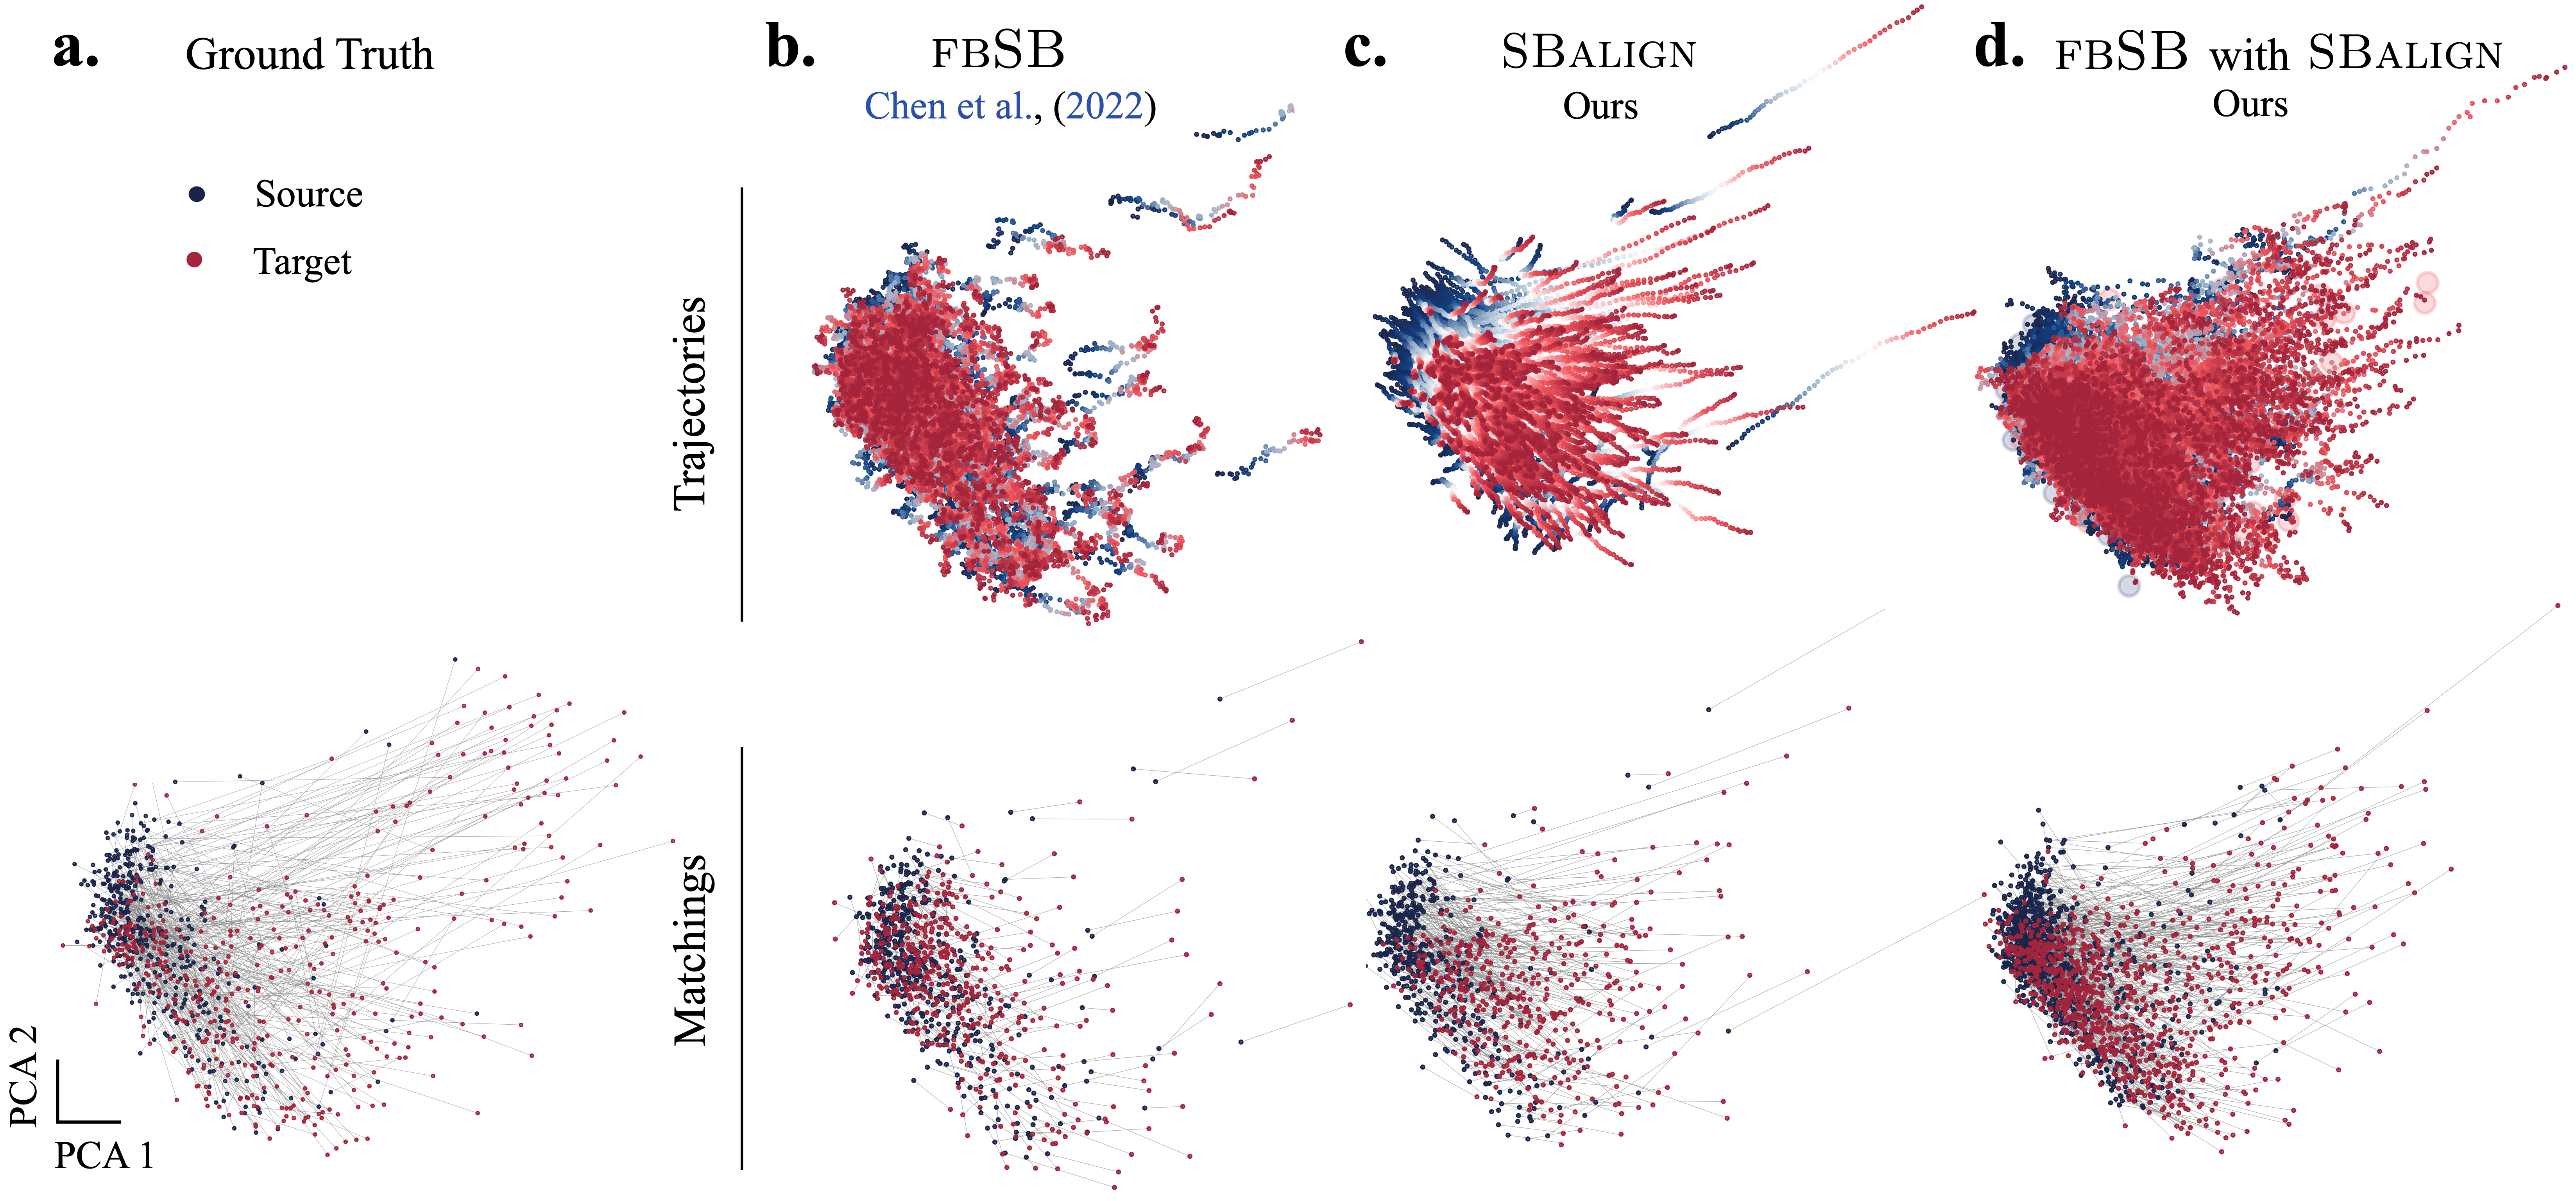
\includegraphics[width=\textwidth]{figures/fig_cell_trajectories_matchings.png}
    \caption{Cell differentiation trajectories based on (\textbf{a}) the ground truth and (\textbf{b-d}) learned drifts. \textsc{SBalign} is able to learn an appropriate drift underlying the true differentiation process while respecting the alignment. (\textbf{d}) Using the learned drift from \textsc{SBalign} as a reference process helps improve the drift learned by other training methods.}
    \label{fig:results_cell_traj}
\end{figure*}

We run our algorithm on two synthetic datasets and compare the results with classic diffusion Schr{\"o}dinger bridge models, i.e., the forward-backward SB formulation proposed by \citet{chen2021likelihood}, herein referred to as \textsc{fbSB}. We equip the baseline with prior knowledge, as elaborated below, to further challenge \textsc{SBalign}.

\paragraph{Moon dataset.}
The first synthetic dataset (\cref{fig:results_spiral}a-c) consists of two distributions, each supported on two semi-circles ($\distinit$ drawn in \textit{blue} and $\distend$ in \textit{red}).
$\distend$ was obtained from $\distinit$ by applying a clockwise rotation around the center, i.e., by making points in the upper blue arm correspond to those in the right red one.
This transformation is clearly not the most likely one under the assumption of Brownian motion of particles and should therefore not be found as the solution of a classical SB problem. 
This is confirmed by \textsc{fbSB} trajectories (\cref{fig:results_spiral}a), which tend to map points to their closest neighbor in $\distend$ (e.g., some points in the upper arm of $\distinit$ are brought towards the left rather than towards the right). 
While being a minimizer of \eqref{eq:SB}, such a solution completely disregards our prior knowledge on the alignment of particles, which is instead reliably reproduced by the dynamics learned by \textsc{SBalign} (\cref{fig:results_spiral}c).

One way of encoding this additional information on the nature of the process is to modify $\refpro$ by introducing a clockwise radial drift, which describes the prior tangential velocity of particles moving circularly around the center.
Solving the classical SB with this updated reference process indeed generates trajectories that respect most alignments (\cref{fig:results_spiral}b), but requires a hand-crafted expression of the drift that is only possible in very simple cases.

\paragraph{T dataset.}
In most real-world applications, it is very difficult to define an appropriate reference process $\refpro$, which respects the known alignment without excessively distorting the trajectories from a solution to \eqref{eq:SB}. This is already visible in simple examples like (\cref{fig:results_spiral}d-f), in which the value of good candidate prior drifts at a specific location needs to vary wildly in time.
In this dataset, $\distinit$ and $\distend$ are both bi-modal distributions, each supported on two of the four extremes of an imaginary T-shaped area.
We target alignments that connect the two arms of the T as well as the top cloud with the bottom one. We succeed in learning them with \textsc{SBalign} (\cref{fig:results_spiral}e) but unsurprisingly fail when using the baseline \textsc{fbSB} (\cref{fig:results_spiral}d) with a Brownian motion prior.

\looseness -1 In this case, however, attempts at designing a better reference drift for \textsc{fbSB} must take into account the additional constraint that the horizontal and vertical particle trajectories intersect (see \cref{fig:results_spiral}e), i.e., they cross the same area at times $t_h$ and $t_v$ (with $t_h > t_v$). This implies that the drift $b_t$, which initially points downwards (when $t < t_v$), should swiftly turn rightwards (for $t > t_h$).
Setting imprecise values for one of $t_h$ and $t_v$ when defining custom reference drifts for classical SBs would hence not lead to the desired result and, worse, would actively disturb the flow of the other particle group.

\looseness -1 As described in \cref{subsec:prior_drift}, in the presence of hard-to-capture requirements on the reference drift, the use of \textsc{SBalign} offers a remarkably easy and efficient way of learning a parameterization of it. For instance, when using the drift obtained by \textsc{SBalign} as reference drift for the computation of the SB baseline (\textsc{fbSB}), we find the desired alignments (\cref{fig:results_spiral}f).

\begin{figure*}[t]
    \centering
    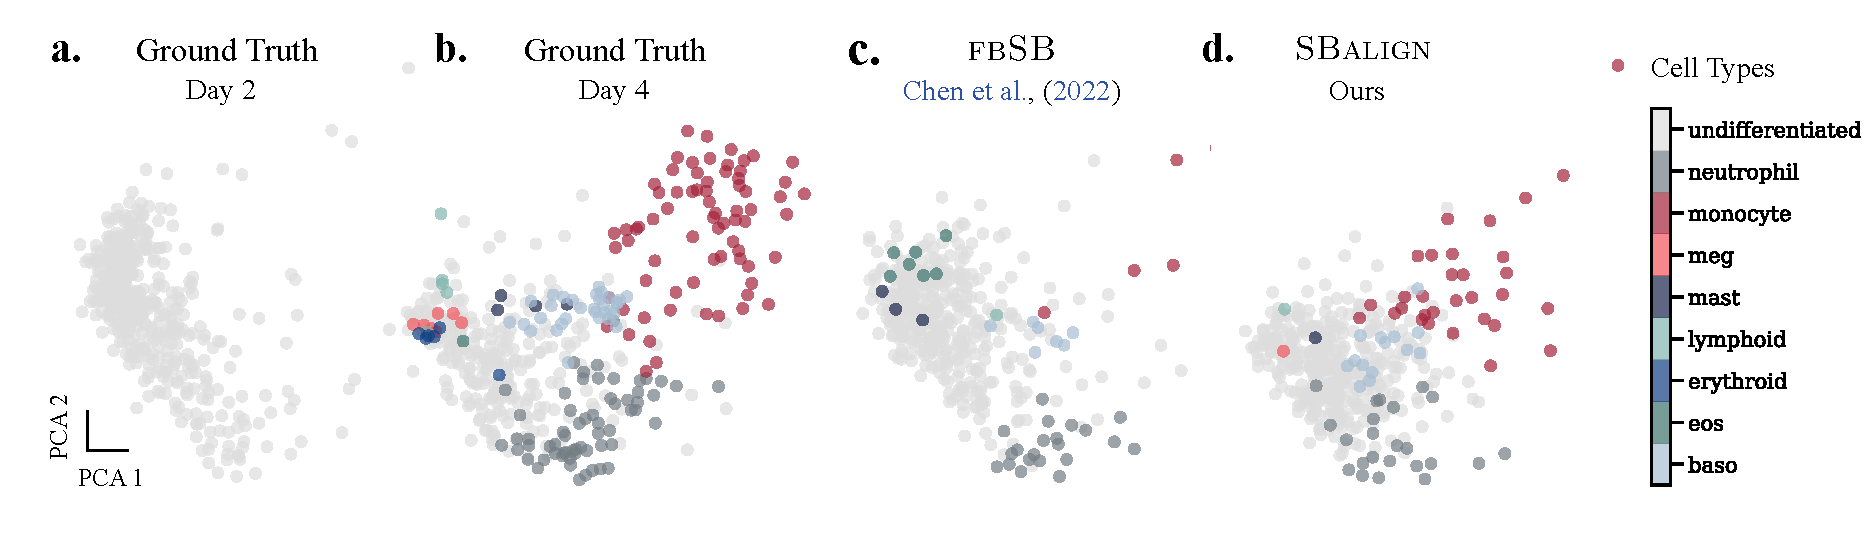
\includegraphics[width=\textwidth]{figures/fig_cell_pred_types.pdf}
    \caption{Cell type prediction on the differentiation dataset. All distributions are plotted on the first two principal components. \textbf{a-b:} Ground truth cell types on day 2 and day 4 respectively. \textbf{c-d:} \textsc{fbSB} and \textsc{SBalign} cell type predictions on day 4. \textsc{SBalign} is able to better model the underlying differentiation processes and capture the diversity in cell types.}
    \label{fig:results_cell_class}
\end{figure*}

\subsubsection{Single-Cell Dynamics}
\label{sec:sbalign_cell}

% \looseness -1 Biological processes are determined through heterogeneous responses of single cells to external stimuli, i.e., developmental factors or drugs. Understanding and predicting the dynamics of single cells subject to a stimulus is thus crucial to enhance our understanding of health and disease and the focus of this task.
Most single-cell high-throughput technologies are destructive assays ---i.e., they destroy cells upon measurement--- allowing us to only measure \textit{unaligned} snapshots of the evolving cell population. Recent methods address this limitation by proposing (lower-throughput) technologies that keep cells alive after transcriptome profiling \citep{chen2022live} or that genetically tag cells to obtain a clonal trace upon cell division \citep{weinreb2020lineage}.

To showcase \textsc{SBalign}'s ability to make use of such (partial) alignments when inferring cell differentiation processes, we take advantage of the genetic barcoding system developed by \citet{weinreb2020lineage}. With a focus on fate determination in hematopoiesis, \citet{weinreb2020lineage} use expressed DNA barcodes to clonally trace single-cell transcriptomes over time. The dataset consists of two snapshots: the first, recorded on day 2 when most cells are still undifferentiated (see \cref{fig:results_cell_class}a), and a second, on day 4, comprising many different mature cell types (see \cref{fig:results_cell_class}b). For details on the dataset, see \cref{app:dataset_weinreb}. Using \textsc{SBalign} as well as the baseline \textsc{fsSB}, we attempt to reconstruct cell evolution between day 2 and day 4, all while capturing the heterogeneity of emerging cell types.

\begin{table}
    \caption{\textbf{Cell differentiation prediction results.} Means and standard deviations (in parentheses) of distributional metrics (MMD, $\text{W}_{\varepsilon}$), alignment-based metrics ($\ell_2$, RMSD), and cell type classification accuracy.}
    \label{tab:results_cells}
     \centering
    \adjustbox{max width=0.85\linewidth}{%
    \begin{tabular}{lccccc}
    \toprule
     & \multicolumn{5}{c}{\textbf{Cell Differentiation}} \\
    \cmidrule(lr){2-6}
    \textbf{Methods} & MMD $\downarrow$ & $\text{W}_\varepsilon \downarrow$ & $\ell_2(\text{PS}) \downarrow$ & RMSD $\downarrow$ & Class. Acc. $\uparrow$ \\
    \midrule
     \textsc{fbSB}& \makecell{1.55e-2\\(0.03e-2)} & \makecell{12.50\\(0.04)} & \makecell{4.08\\(0.04)} & \makecell{9.64e-1\\(0.02e-1)} & \makecell{56.2\%\\(0.7\%)} \\
     \textsc{fbSB} with \textsc{SBalign} & \makecell{5.31e-3\\(0.25e-3)} & \makecell{10.54\\(0.08)} & \makecell{0.99\\(0.12)} & \makecell{9.85e-1\\(0.07e-1)} & \makecell{47.0\%\\(1.5\%)} \\
     \textsc{SBalign} & \makecell{1.07e-2\\(0.01e-2)} & \makecell{11.11\\(0.02)} & \makecell{1.24\\(0.02)} & \makecell{9.21e-1\\(0.01e-1)} & \makecell{56.3\%\\(0.7\%)} \\
     \bottomrule
    \end{tabular}
}
\end{table}

We benchmark \textsc{SBalign} against previous \acrshortpl{DSB} such as \citep[\textsc{fbSB}]{chen2021likelihood}. Beyond, we compare \textsc{SBalign} in the setting of learning a prior reference process. Naturally, cell division processes and subsequently the propagation of the barcodes are very noisy. While this genetic annotation provides some form of assignment, it does not capture the full developmental process. We thus test \textsc{SBalign} in a setting where it learns a prior from such partial alignments and, plugged into \textsc{fbSB}, is fine-tuned on the full dataset.
To assess the performance of \textsc{SBalign} and the baselines, we monitor several metrics, which include distributional distances, i.e., MMD~\citep{gretton2012kernel} and $\text{W}_{\varepsilon}$~\citep{cuturi2013sinkhorn}, as well as average \acrfull{PS}, i.e., $\ell_2(\text{PS})$, and \acrfull{RMSD}. Details on the considered evaluation metrics can be found in \cref{app:evaluation_metrics}.
Moreover, we also train a simple neural network-based classifier to annotate the cell type on day 4 and we report the accuracy of the predicted vs. actual cell type for all the models.


\textsc{SBalign} finds matching between cell states on days 2 and 4 (\cref{fig:results_cell_traj}c, bottom) which resemble the observed ones (\cref{fig:results_cell_traj}a) but also reconstructs the entire evolution path of transcriptomic profiles (\cref{fig:results_cell_traj}c, top).
It outperforms the baseline \textsc{fbSB} (Table \ref{tab:results_cells}) in all metrics: Remarkably, our method exceeds the performances of the baseline also on distributional metrics and not uniquely on alignment-based ones.
We also leverage \textsc{SBalign} predictions to recover the type of cells at the end of the differentiation process (\cref{fig:results_cell_class}d). We do that by training a classifier on differentiated cells observed on day 4 and subsequently classify our predictions. % and applying it to cell statuses predicted by our method.
While capturing the overall differentiation trend, \textsc{SBalign} (as well as \textsc{fbSB}) struggles to isolate rare cell types.
Lastly, we employ \textsc{SBalign} to learn a prior process from noisy alignments based on genetic barcode annotations. When using this reference process within \textsc{fbSB}, we learn an SB which compensates for inaccuracies stemming from the stochastic nature of cell division and barcode redistribution and which achieves better scores on distributional metrics (see Tab.~\ref{tab:results_cells}).

\textsc{SBalign} accurately predicts cellular differentiation processes in hematopoiesis from day 2 to day 4, as visible from the (2D projections of the) learned trajectories and alignments (\cref{fig:results_cell_traj}c) and the quantitative evaluation in Table~\ref{tab:results_cells}. \textsc{SBalign} outperforms \textsc{fbSB} in all but the cell-type accuracy metric: Remarkably, our method exceeds the performances of the baseline also on distributional metrics and not uniquely on alignment-based ones. Further, we evaluate how well \textsc{SBalign} recovers the heterogeneity of emerging cell types throughout the developmental process on day 4. The results are displayed in \cref{fig:results_cell_class}d and show that, while capturing the overall differentiation trend, \textsc{SBalign} (as well as \textsc{fbSB}) struggles to isolate rare cell types.
Lastly, we employ \textsc{SBalign} to learn a prior process from noisy alignments based on genetic barcode annotations. When using this reference process within \textsc{fbSB}, we learn an SB which compensates for inaccuracies stemming from the stochastic nature of cell division and barcode redistribution and which achieves better scores on distributional metrics (see \cref{tab:results_cells}).

\subsection{Discussion}

In this section, we propose a new framework to tackle the interpolation task with aligned data via \acrlongpl{DSB}. Our central contribution is a novel algorithmic framework derived from the Schr{\"o}dinger bridge theory and Doob's $h$-transform. Via a combination of the two notions, we derive novel loss functions which, unlike all prior methods for solving \acrlongpl{DSB}, do not rely on the \acrlong{IPF} procedure and are hence numerically stable. We verify our proposed algorithm on various synthetic and real-world tasks and demonstrate noticeable improvement over the previous state-of-the-art, thereby substantiating the claim that data alignment is a highly relevant feature that warrants further research.


\cleardoublepage%
\chapter{Conclusion and Future Directions}
\label{cha:conclusion}

\dictum[Siri Hustvedt, \textit{What I Loved} (2003)]{%
  It's odd the way life works, the way it mutates and wanders, the way one thing becomes another.}%
% \dictum[Siri Hustvedt, \textit{The Shaking Woman, \\ or A History of My Nerves} (2010)]{True stories can't be told forward, only backward. We invent them from the vantage point of an ever-changing present and tell ourselves how they unfolded.}
\vskip 2em

Optimal transport, both through its theory and computation, has enabled breakthroughs using a multi-pronged approach, blending elements from convex optimization, e.g., linear and quadratic assignment problems, the Sinkhorn algorithm; analysis, e.g., partial differential equations \citep{jordan1998variational, bunne2022proximal} with links to Monge-Amp{\`e}re equation \citep{caffarelli2003monge}; stochastic calculus, e.g., diffusion models \citep{song2020score}, Schr{\"o}dinger bridge \citep{de2021diffusion, chen2021likelihood, bunne2022recovering}; statistics, e.g., analysis of sampling algorithms \citep{weed2019sharp}, generalized quantiles \citep{carlier2016vector, cuturi2019differentiable}, generative model fitting \citep{salimans2018improving, genevay2018learning, bunne2019learning, bunne2021learning}; and deep architectures \citep{de2019stochastic}.
As such, it provides a unifying framework for modeling population dynamics through maps (\cref{sec:background_monge}), as well as ordinary (\cref{sec:background_benamou_brenier}), partial (\cref{sec:background_jko}), or stochastic differential equations (\cref{sec:background_sb}). 
This thesis thereby introduced (\colcircle{blue}) neural network-based parameterization of these different flavors of OT and demonstrated their far-reaching applications in the field of biomedicine.
% TODO: Rework.
The proposed algorithms thereby build on the recent successes of optimal transport applications in single-cell biology \citep{schiebinger2019optimal, lavenant2021towards}. 
Through its ability to realign (\colcircle{pink})  distributions and model their evolution over time, OT is able to (\colcircle{lightblue}) reconstruct single-cell dynamics from distinct and unpaired measurements.
Thus, by adequately modeling the nature of single-cell dynamics (\colcircle{darkblue}) through appropriate inductive biases, % through the lens of optimal transport, 
these methods allow us to  determine how perturbations affect cellular properties, reconstruct the most likely trajectory single cells take upon perturbation, and subsequently assist in a better understanding of driving factors of cell fate decision and cellular evasion mechanisms.
These methods are now an integral part of open-source libraries \citep{cuturi2022optimal, klein2023mapping} and show strong quantitative improvements and an increase in robustness to noise, making them applicable to high-dimensional single-cell data.

In the following, we summarize the contributions of this thesis, discuss current limitations and open questions, and provide an outlook on an exciting avenue of future work.

\section*{Contributions and Summary}

Let us revisit the following core questions this thesis has aimed to address:

\subsubsection*{\textbf{How to learn dynamic treatment responses at the single cell level and make predictions to unseen patients?}}

\looseness -1 Learning perturbation responses of an existing patient cohort enables inference of treatment responses for new, previously unseen patients, assuming that we capture the heterogeneous drug reactions of patients during training.
We thus seek to learn a perturbation model that robustly describes the cellular dynamics upon intervention while still accounting for underlying variability across samples.
My approach to this problem learns a neural map that aligns the control and perturbed cell population by leveraging the theory of optimal transport and the recent advent of convex neural architectures \citep{bunne2021learning}.
% This map then best describes the incremental changes in the multivariate profile of each cell after applying a perturbation through parameterizing the pair of OT dual potentials using convex neural networks.
By inducing an important theory-motivated inductive bias essential to model stability, these approaches outperforms prior methods in predicting heterogeneous tumor cell responses to a diverse set of cancer drugs and is currently employed to predict treatment outcomes of a large clinical study \citep{irmisch2021tumor}.

Beyond mappings, OT provides a mathematical link to geometric variational frameworks that allow studying flows of distributions on metric spaces.
% Recent work of mine models cellular dynamics as control problems described through systems of stochastic \citep{bunne2022recovering} or partial differential equations \citep{bunne2022proximal}.
In particular, I proposed a causal model for population dynamics relying on the Jordan-Kinderlehrer-Otto (JKO) flow, widely regarded as one of the most influential mathematical breakthroughs in recent history. By modeling dynamics as a gradient flow, cells decrease collectively an energy which one seeks to learn (i.e., the Waddington potential) \citep[\textrm{i.}]{bunne2022proximal}. 

Cell fate decisions are of stochastic nature and cellular dynamics intrinsically noisy \citep{wilkinson2009stochastic}.
Approaches treating cell fate decisions as probabilistic events have previously allowed estimation of the full dynamical model to a greater extent than their deterministic counterparts \citep{bergen2020generalizing}.
By connecting OT and stochastic difference equations, recent work \citep{bunne2022recovering, somnath2023aligned} can build up on \textsc{CellOT} to account for biological heteroscedasticity.
Alternatively, we can thus recover a system of differential equations that best describes the stochastic transitions between cell fates in developmental processes \citep{bunne2022recovering, somnath2023aligned}.
Beyond broadening the spectrum of existing methods for cell dynamics, my work incorporates theoretically well-motivated priors that make these approaches more robust to noise and increases performance compared to existing approaches.

\subsubsection*{\textbf{How to predict the outcome of combination therapies and adapt our tools to scalable high-resolution methods?}}

\looseness -1 While these models can predict cell perturbation responses to single drugs, a key challenge in the treatment of many diseases is to predict the effect of combination therapies. Besides the algorithmic challenge, the space of possible combinations is much vaster than the number of cells one can measure, resulting in highly under-sampled experiments. To scale up the experimental capacity, recent studies have resorted to random and composite experiments \citep{norman2019exploring, cleary2020necessity}.
This thesis has thus focused on proposing a general framework that allows us not only to predict the outcomes of combination treatments but also train models on random, composite experiments \citep{bunne2022supervised}.
We achieve this by learning a parametric family of context-aware transport maps instead of individual maps for each condition.
The approach trains a single data-efficient model for all perturbations and respective combinations, where the considered setting is passed as a context variable to the model. This allows us to predict the outcomes of combination therapies and is in line with the setup of random, composite large-scale experiments.
Further, the learned map can generalize to unseen combination therapies once trained on similar contexts.


% These concepts enable us to predict a patient's response to chemical or genetic perturbations and model responses to therapies applied in combination. This paves the way for \textit{in silico} screening of potential drug candidates or inferring outcomes of treatment strategies for unseen patients.
% Before this is possible, an analysis of a drug candidate on a more macromolecular level is necessary: Once potential drug candidates are identified, we need to understand their interaction to target proteins \citep{ganea2021independent} and derive synthesis plans from initial reactants \citep{schwaller2022machine, somnath2021learning}. 


\section*{Limitations}

Single-cell expression profiling provides a detailed look into the molecular states of individual cells, but it is destructive and does thus not allow continuous measurements of molecular properties over time. There have been numerous proposals for methods to uncover the dynamics of individual cells from population data, but all of them face the same challenge: Sequentially observed distribution of cell states can be produced by multiple dynamics and mechanisms of gene regulation. The ill-defined nature of the problem makes it necessary to pose certain assumptions on the underlying cellular dynamics.

The mathematical foundation of this work builds on the biological intuition that perturbations incrementally alter the molecular profiles of cells. 
If this principle is violated, however, and perturbations strongly disrupt the population to an unidentifiable level, the performance of optimal transport-based algorithms ... as well as other methods drops.
In these instances, more complicated mathematical machinery would be needed.
Such tools, however, are currently unable to scale to settings with more than a few genes \citep{heydari2022iqcell}.
Thus, we rely on a fine granularity of the time course to recover large cell state changes between consecutive time points \citep{tritschler2019concepts}.

We also observe that the predictive performance of neural optimal transport methods drops when perturbations are too strong, i.e., the cell distributions before and after perturbations are very different (see \cref{fig:generalization_cellot}j); a similar drop is observed for the other methods.
The principle underlying the optimal transport theory is ideally suited for acute cellular perturbations during which single cells do not redistribute entirely and randomly in multidimensional measurement space, but typically only in a few dimensions, such that the overall correlation structure is preserved. While this modeling hypothesis is satisfied when perturbation responses are observed via regularly and frequently sampled snapshots, molecular transitions cannot be reconstructed when perturbation responses have progressed too far. For particularly strong or complicated perturbations, cellular multiplex profiles might change too drastically, violating OT assumptions and making it challenging to reconstruct the alignments between unperturbed and perturbed populations based on the \emph{minimal effort} principle.
In such settings, additional information is likely needed, for instance, a model of the underlying biology or models that integrate observations of multiple smaller time steps. 

Furthermore, if a system exhibits rotations and oscillations within two consecutive snapshots not captured by measurements, models based on optimal transport and previous tools \citep{weinreb2018fundamental} will not be able to recover such complex dynamics. This is in part also due to the current choice of the cost function, which, due to theoretical constraints and practical performance, is set to the Euclidean distance. We leave it to future work, to investigate choices of alternative cost functions. 

Beyond, the current system is not able to recover effects (other than cell flux) that change the distribution of cells between time points, for example, proliferation and death \citep{tritschler2019concepts}. Recent works propose extensions to the classical neural optimal transport scheme that account for cell death and birth \citep{lubeck2022neural, pariset2023unbalanced, chen2022most, baradat2021regularized}.

Despite having provided a proof-of-concept of the capacity of \textsc{CellOT} to model various chemical perturbations for different data modalities through an in-depth analysis of the nature of the learned mapping as well as a demonstration of its versatility in a broad class of applications, the generalization capacity of the proposed methods has been evaluated on relatively small datasets. Crucially, large cohorts comprised of patients with different molecular profiles, such as cancer patients with various underlying genetics, could result in strongly heterogeneous treatment responses.
It is evident that approaches addressing these challenges could readily exploit the upcoming availability of large-scale patient cohort studies.

\section*{Future Directions and Conclusion}

The challenges posed by the inherently complex and constantly changing patterns of interactions in biological systems call for innovative computational solutions. Through the development of static and dynamic neural optimal transport schemes, this thesis has laid a solid foundation for addressing these challenges.
...
% The use of neural optimal transport to learn single-cell drug responses makes thus for an exciting avenue for future work, including its use to improve our understanding of cell therapies, study drug responses from patient samples, and better account for cell-to-cell variability in large-scale drug design efforts.

\subsubsection*{\textbf{Does knowledge of chemical and genetic perturbation responses help us to identify new drug targets?}}

Which genetic perturbation is connected to a drug's mode of action? Given a genetic cause of disease, which drug should be selected for the successful treatment of a patient?
\cref{cha:cellot} and \cref{cha:condot} contributed to our understanding of heterogeneous single-cell responses to chemical and genetic perturbations \citep[]{bunne2019learning, bunne2022supervised}.
Understanding similarities and detecting correspondences between the genetic roots of the disease and the mode of action of chemical drugs are key to the discovery of targets for which new drugs need to be designed.
While optimal transport can be used to describe the evolution of probability measures, one can rely on its ability to return a matching based on the structural similarity of objects \citep{bunne2019learning}, making it a centerpiece for solving this task.
Building on intuitions acquired when solving matching problems of unaligned cell populations, future research will develop OT-based machine learning algorithms to identify novel targets for drug development.


\subsubsection*{\textbf{How to develop methods embracing the nature of massively parallelized high-throughput methods?}}

For decades, experimental biology required us to specifically select the targets we want to observe. Modern massively parallelized high-throughput methods have made it possible to measure thousands of such targets (possibly in combination) in one experiment and collect rich information about the gene expression profiles of each cell.
Current computational methodology, however, is often overwhelmed with this depth of data resolution.
In \cref{cha:condot}, we have provided methods that can deal with the randomized and composite nature of approaches, such as compressed Perturb-Seq \cite{dixit2016perturb, cleary2017efficient, cleary2020necessity, roohani2022gears}.
But our work does not end there: With the rise of new methodologies such as Live-seq \citep{chen2022live} or added levels of dimensions through spatial transcriptomics \citep{marx2021method}, we need to drive the design of machine learning algorithms even further (\cref{sec:sbalign}). Disease can not be solely modeled from the single-cell perspective, but emerges in tissues. Modeling tissue structures and interactions by utilizing principles of geometric deep learning holds the promise to further unveil mechanisms of human disease and thus makes for an exciting avenue of future work.


\subsection*{\textbf{What are objective milestones toward end-to-end machine learning-guided treatment discovery and planning?}}

This thesis has evolved around achieving the trifecta of (i.) theory-inspired and (ii.) modular deep learning architectures (iii.) with appropriate inductive biases. Integrating these paradigms into machine learning methods that operate on various challenges of treatment discovery and planning has allowed novel biological insights and created a new state-of-the-art: OT lets us predict meaningful perturbation responses of a patient on the level of single cells \citep{bunne2021learning, bunne2022supervised}, and thus improves our understanding of disease mechanisms by deciphering the underlying molecular processes \citep{bunne2022proximal, bunne2022recovering}. Further, predicting geometrically valid conformations of a drug-target pair increases the accuracy of current drug design pipelines \citep{somnath2021multi, ganea2022independent, somnath2023aligned}. \\

This provides fertile grounds to start asking bigger questions: How can we incorporate insights made from predicting a patient's drug response into target discovery \citep{huang2022artificial}? Or, inversely, how to use knowledge of drugs and their connected targets when designing personalized treatment plans \citep{nilforoshan2023zero}? Building on recent developments in reinforcement learning and control theory, how do we innovate the design of personalized, sequential combination therapies for patients?
These questions reveal that we cannot address the different challenges that arise throughout the drug design process in isolation.
Taking this thesis as a starting point, future work will focus on developing mathematical and computational principles for end-to-end machine learning-guided treatment discovery and planning:
By designing feedback loops that allow information sharing across different modules of drug design. \\


% The unified framework introduced here promises exciting opportunities for novel biological discoveries, personalized therapies, and regenerative medicine. 
% By interweaving the threads of theory, methodology, application, and future potential, this thesis serves as a testament to the transformative power of interdisciplinary research and innovation in the pursuit of understanding and harnessing the complexity of life.


\newpage
{
\renewcommand*{\bibfont}{\normalfont\footnotesize}
\bibliographystyle{plainnat}
\bibliography{references.bib}
}

\bookmarksetup{startatroot}
\cleardoublepage%*******************************************************
% CV
%*******************************************************
\pdfbookmark[1]{Curriculum Vitae}{cv}

\bigskip

\begingroup
\let\clearpage\relax
\let\cleardoublepage\relax
\let\cleardoublepage\relax
\chapter*{Curriculum Vitae}

{ \small
\section*{Personal Data}
\vspace{-3pt}

\noindent\cvleft{Name}%
\cvright{Charlotte Bunne}\\
%
\cvleft{Date of Birth}%
\cvright{August 29, 1995}\\
%
\cvleft{Place of Birth}%
\cvright{Karlsruhe, Germany}\\
%
\cvleft{Citizen of}%
\cvright{Germany}

\section*{Education}
\vspace{-3pt}

\noindent\cvleft{2019 --~2023}%
\cvright{%
  Eidgen\"ossische Technische Hochschule (ETH), \\
  Z\"urich, Switzerland \\
  \emph{Final Degree:} Doctor of Science
}\vspace{0.75em}

\noindent\cvleft{2022-2023}%
\cvright{%
  Broad Institute of MIT and Harvard,\\ Cambridge (MA), USA \\
  Visiting Graduate Student
}\vspace{0.75em}

\noindent\cvleft{2016 --~2019}%
\cvright{%
  Eidgen\"ossische Technische Hochschule (ETH), \\
  Z\"urich, Switzerland \\
  \emph{Final Degree:} Master of Science
}\vspace{0.75em}

\noindent\cvleft{2018-2019}%
\cvright{%
  Massachusetts Institute of Technology (MIT), \\
  Cambridge (MA), USA \\
  Visiting Student
}\vspace{0.75em}

\noindent\cvleft{2013 --~2016}%
\cvright{%
  Heidelberg University \\
  Heidelberg, Germany \\
  \emph{Final Degree:} Bachelor of Science
}\vspace{-0.75em}

\section*{Employment}
\vspace{-3pt}

\noindent\cvleft{2022}%
\cvright{%
  Research Intern \\
  \emph{Apple},\\ Paris, France
}\vspace{0.75em}

\noindent\cvleft{2020}%
\cvright{%
  Research Intern \\
  \emph{Google Research},\\ Z{\"u}rich, Switzerland
}\vspace{0.75em}

\noindent\cvleft{2017}%
\cvright{%
  Research Intern \\
  \emph{IBM Research},\\ Z{\"u}rich, Switzerland
}\vspace{0.75em}
}

\endgroup

\cleardoublepage%*******************************************************
% Publications
%*******************************************************
\pdfbookmark[1]{Publications}{publications}
\chapter*{Publications}

\nociteown{*}

\def\bibsection{\section*{\refname}} 

{
\thispagestyle{empty}
\let\clearpage\relax
\bibliographystyleown{plainnat}
\bibliographyown{ownpubs}
}

\appendix
\cleardoublepage%
\chapter{Appendix}
\label{cha:appendix}

\section{Further Empirical Evaluation}

\begin{figure}[H]
     \centering
     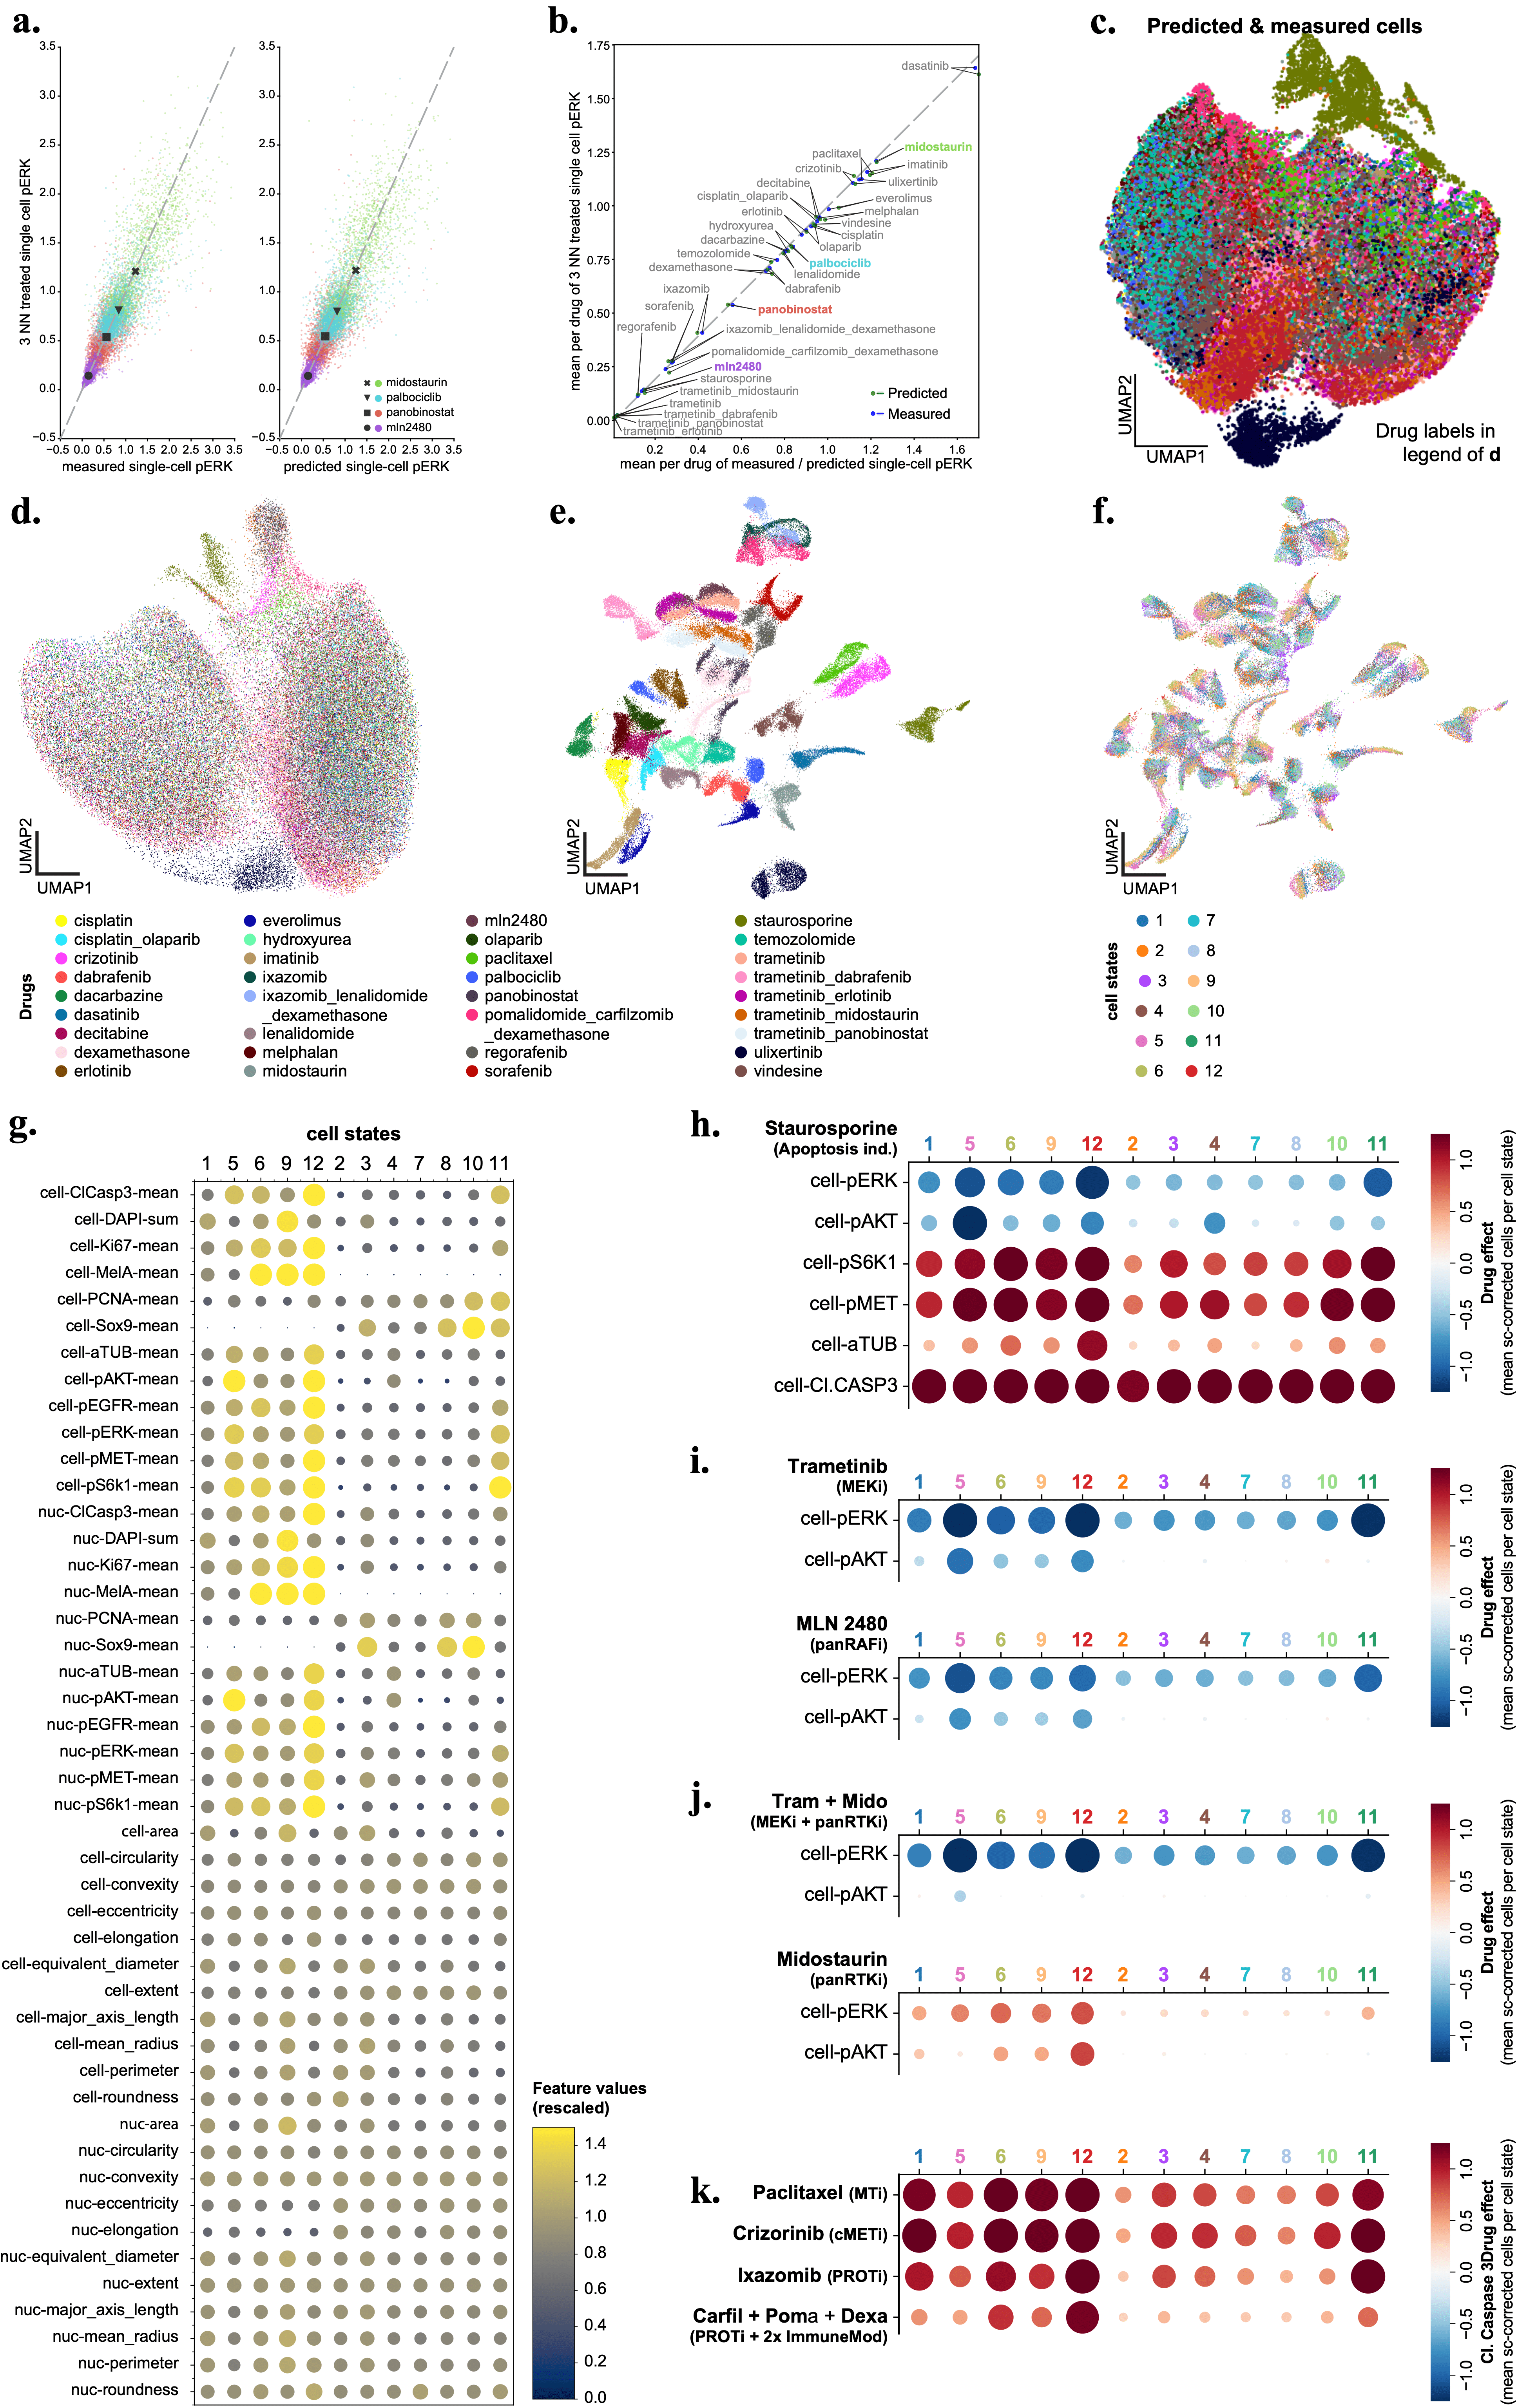
\includegraphics[height=.95\textheight ]{figures/fig_4i_analysis_extended.png}
\end{figure}
\captionof{figure}{
\textbf{a.} High similarity of measured and CellOT-predicted \acrlong{sc} pERK (phosphor ERK1/2) values at the \acrlong{sc} level. Scatter plots compare the relationship between measured pERK values of cells (left) treated with Midostaurin (green dots), Palbociclib (blue dots), Panobinostat (red dots), and MLN2480 (purple dots) or (right) predicted for those drugs along the horizontal axis to their corresponding 3NN cells on the vertical axis. X mark, square, inverted triangle, and circle represent the mean of the respective measurements per drug. The dashed gray line indicates the diagonal along which the measurements would correlate perfectly. \textbf{b.} The high similarity of measured and CellOT-predicted \acrlong{sc} pERK (phosphor ERK1/2) values at the population level across all drug perturbations. Drug average of measured (blue dots) and predicted (green dots) pERK values compared to their respective 3NN measurement. Drug treatments highlighted in color correspond to those presented in panel \textbf{a.}. The dashed gray line indicates the diagonal along which the measurements would correlate perfectly. \textbf{c.} Projection of measured perturbed and predicted perturbed cells in a shared \acrshort{UMAP} space. Each cell is color-coded according to the perturbation from which it originates. \textbf{d.} Projection of mean-corrected measured perturbed cells in a \acrshort{UMAP} space. Each cell is color-coded according to the perturbation from which it originates. A mean correction was achieved by subtracting the mean of every feature for all cells in the control condition and subtracting the calculated feature means from the feature values of individual cells. \textbf{e.} Projection of \acrlong{sc} corrected, predicted perturbed cells in a \acrshort{UMAP} space. Each cell is color-coded according to the perturbation model with which it was predicted. \textbf{f.} Projection of \acrlong{sc} corrected, predicted perturbed cells in a \acrshort{UMAP} space. Each cell is color-coded according to its assignment to one of the 12 cell states. \textbf{g.} Feature value overview of the 12 identified cell states in DMSO-treated (control) cells. Each column represents a cell state, and each row a feature. Circles are colored and scaled based on feature value, from small size in blue for low feature values, to large circles in yellow for high feature values. \textbf{h-j.} Drug effect overview of the 12 identified cell states in \textbf{h.} Staurosporine (apoptosis ind.m apoptosis inducer, \textbf{i.} Trametinib (MEKi, MEK inhibitor), MLN2480 (panRAFi, panRAF inhibitor), \textbf{j.} Trametinib + Midostaurin (Tram + Mido, MEK inhibitor + pan Receptor Tyrosine Kinase inhibitor (panRTK)), Midostaurin (panRTK). Each column represents a cell state, and rows represent features. "cell-" stands for mean cell intensity. Circles are scaled based on drug effect, the larger the $\pm$ effect the larger the circles. Negative values are encoded in hues of blue, and positive values in red hues of the respective circles. \textbf{k.} Effect of drug treatments on levels of cleaved Caspase 3 (cleaved Caspase 3) in the 12 identified cell states. Each column represents a cell state, and each row a drug treatment.}
\label{fig:4i_analysis_extended}

\newpage
\begin{figure}[H]
     \centering
     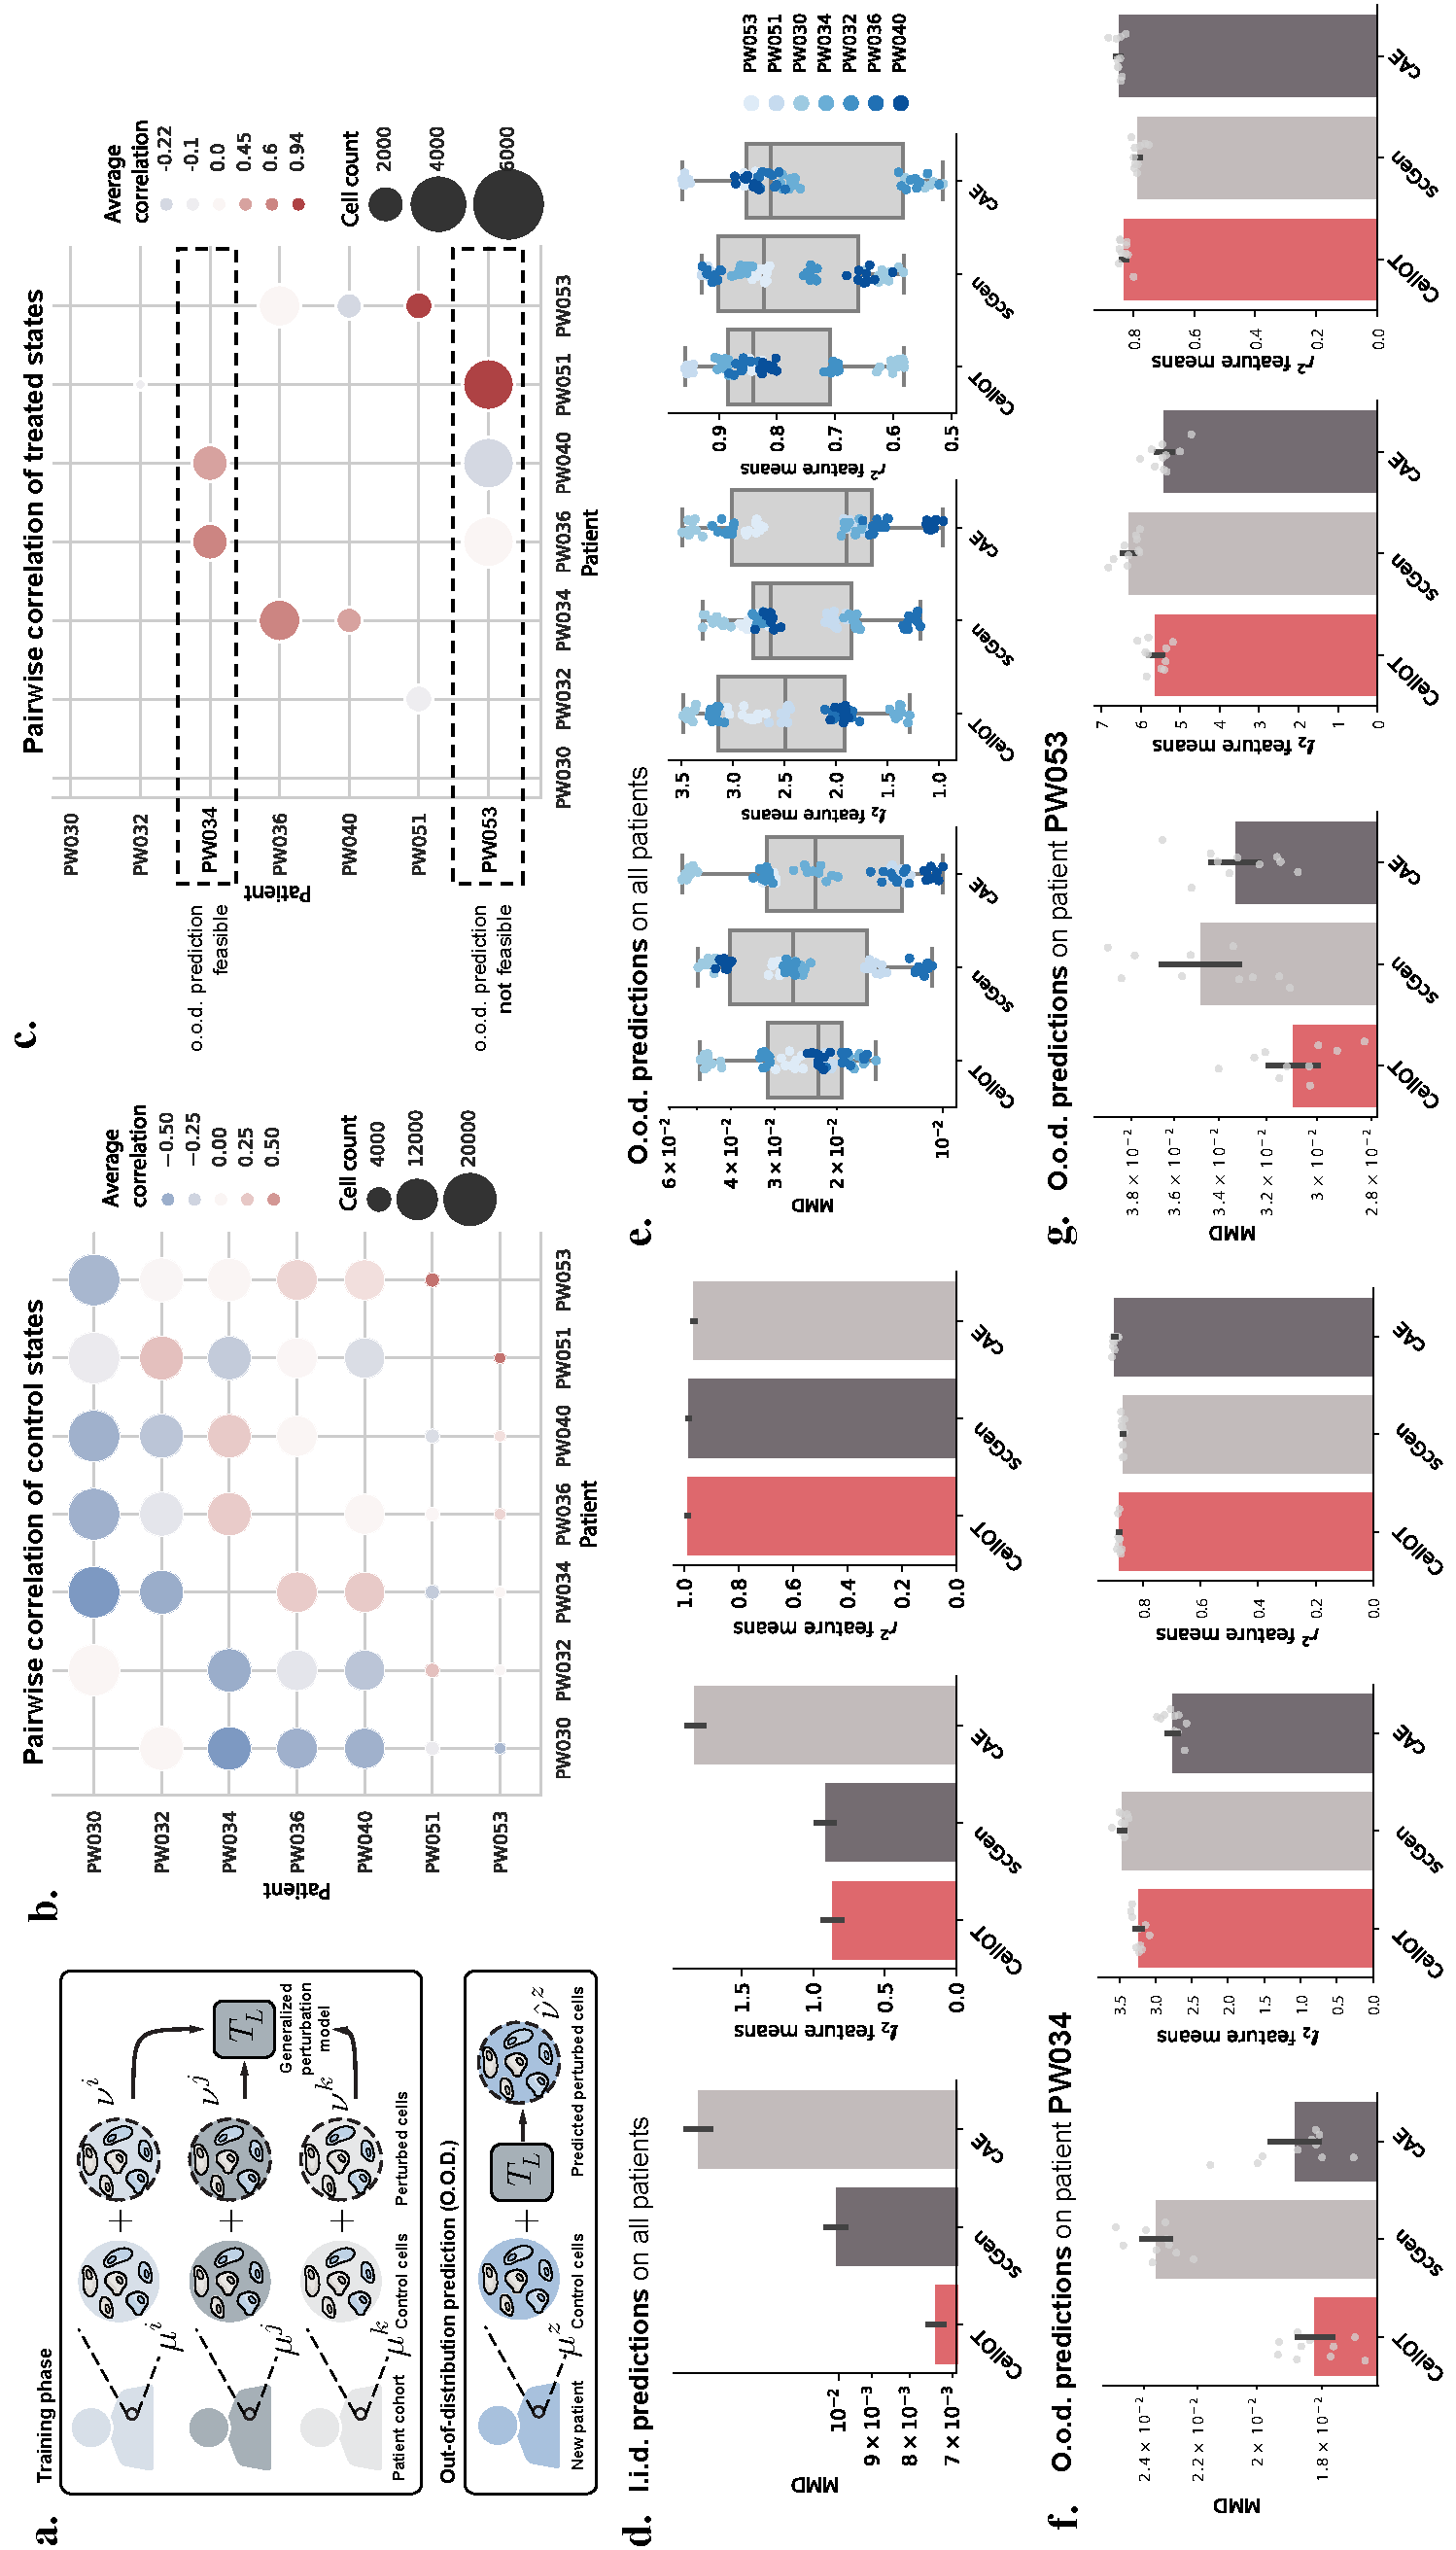
\includegraphics[width=0.8\textwidth]{figures/fig_gbm_patients_iid_ood.pdf}
\end{figure}
\captionof{figure}{Analysis and results of the glioblastoma dataset consisting of seven patients. \textbf{a.} Cells from seven glioblastoma patients are measured in an untreated and Panobinostat-treated state. For each sample, we train two models, an \acrshort{ood}~model trained on cells from all other samples but the holdout patient we test on and an \acrshort{iid}~model trained with additional access to half of the cells in the holdout sample.
    \textbf{b.} Pairwise average correlation of the \acrshort{PCA} embeddings of the control states between patients. \textbf{c.} Pairwise average correlation of the \acrshort{PCA} embeddings of the treated states between patients, masked to only those patient pairs that showed a positive correlation in the control states. Only patient PW034 positively correlates with all other patients. Other patients, such as PW053, correlate and anti-correlate with other patients in the treated state. Performance comparison between \textsc{CellOT} and baselines for different metrics in the \textbf{d.} \acrshort{iid} setting (mean standard deviation across 7 samples, 10 bootstraps of the test set per sample),
    \textbf{e.} \acrshort{ood} setting for all patients (box plots show median, minima, and maxima)
    \textbf{f.} \acrshort{ood} setting for a patient positively correlating with all patients that are also similar in the control state,
    \textbf{g.} \acrshort{ood} setting for a patient where similar patients in the control state show different responses (correlation and anti-correlation) in the treated states. Data in \textbf{f} and \textbf{g} are presented as the mean +/- standard deviation across n=10 bootstraps of the test set.}
\label{fig:gbm_patients_iid_ood}

\clearpage
\newpage

\begin{figure}[H]
     \centering
     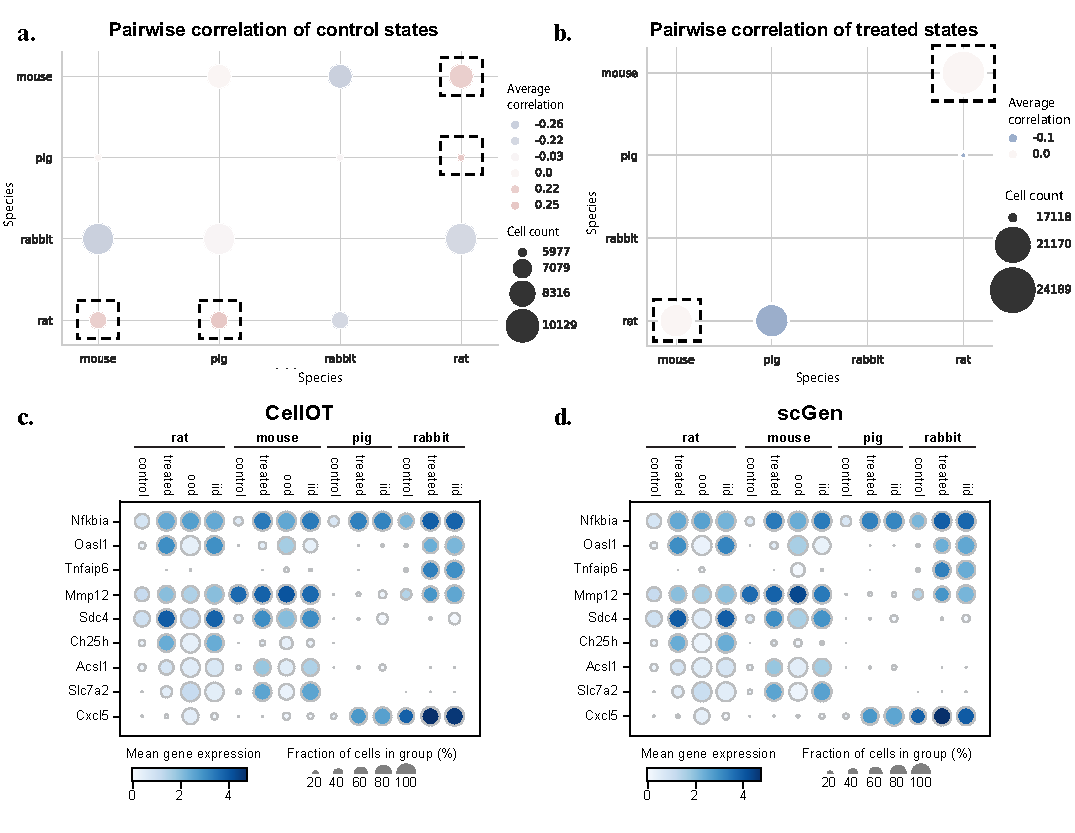
\includegraphics[width=\textwidth]{figures/fig_crossspecies_ood_analysis.pdf}
     \caption{\looseness -1 Analysis and further results of the cross-species dataset. \textbf{a.} Pairwise average correlation of the \acrshort{PCA} embeddings of the control states between species. \textbf{b.} Pairwise average correlation of the \acrshort{PCA} embeddings of the treated states between patients, masked to only those patient pairs that showed a positive correlation in the control states. Only rat and mouse show consistent responses, i.e., a positive correlation of the control states and a non-negative correlation of the respective target cells, and are thus chosen for the \acrshort{ood} analysis. \acrshort{iid} and \acrshort{ood} results measured in the average gene expression for both \textbf{d.} \textsc{CellOT} and \textbf{c.} \textsc{scGen}.}
     \label{fig:crossspecies_ood_analysis}
\end{figure}

\section{Datasets} \label{app:datasets}

We evaluate methods introduced in this thesis on different tasks, each consisting of a pair of source $\mu$ and target measure $\nu$.
In particular, we consider \acrlong{sc} datasets in which populations of single cells have been monitored with modern high-throughput methods such as \acrshort{sc}\acrshort{RNAseq} or optical phenotyping technologies (see \cref{sec:tech_background}).
In the following, we introduce each dataset, describe preprocessing steps, feature selection, and data splits.

\subsection{\citet{srivatsan2020massively}}
\label{app:dataset_srivatsan}

\looseness -1 Cancer drugs reduce uncontrolled cell growth and proliferation by inhibiting \acrshort{DNA} replication and \acrshort{RNA} transcription as well as targeting proteins crucial for cancer progression. In doing so, they modulate downstream signaling cascades, affect cell growth and morphology, and alter gene expression profiles of single cells. 
\citet{srivatsan2020massively} conduct a \acrshort{sc}\acrshort{RNAseq}-based phenotyping screen of transcriptional responses to thousands of independent perturbations at \acrlong{sc} resolution.
The measured cell population contains three well-characterized cancer cell lines, including A549, a human lung adenocarcinoma, K562, a chronic myelogenous leukemia, and MCF7, a mammary adenocarcinoma cell line.
Due to the different transcriptional profiles of each cancer cell line, drug compounds might cause divergent cellular responses in each subpopulation.
The dataset contains $17,565$ control cells as well as a varying number of cells perturbed by different drugs with different dosages, i.e., $10\,$nM, $100\,$nM, $1,000\,$nM, $10,000\,$nM.

\paragraph{Data preprocessing.}
The dataset is available for download in the \acrfull{GEO} database under accession number \href{https://www.ncbi.nlm.nih.gov/geo/query/acc.cgi?acc=GSM4150378}{GSM4150378}.
For data quality control and preprocessing, we follow the analysis of \citet{lotfollahi2021compositional}. The count matrix obtained from \acrshort{GEO} consists of $581,777$ cells. The data were subset to half its size, with $290,888$ cells remaining after quality control for all $188$ different compounds. We proceeded with log transformation and the selection of $1,000$ \acrlongpl{HVG} using \texttt{scanpy} \citep{wolf2018scanpy}.

\paragraph{Feature selection.}
\acrshort{sc}\acrshort{RNAseq} data is very high-dimensional, even after selecting $1,000$ \acrshortpl{HVG}.
For the downstream analysis of how well the overall perturbation effect has been captured, we thus select the top $50$ marker genes, i.e., those genes that show strong differences between perturbed and unperturbed states. This analysis is conducted based on the \texttt{scanpy}'s function \texttt{rank\_genes\_groups}, setting unperturbed cells as reference ~\citep{wolf2018scanpy}. The influence of the number of considered marker genes on different evaluation metrics is further analyzed in \citet{bunne2021learning}.

\subsection{\citet{bunne2021learning}}
\label{app:dataset_bunne}

Besides sc\acrshort{RNAseq}, optical phenotypic screens, e.g., multiplexing tools such as \acrshort{4i} \citep{gut2018multiplexed}, are able to capture meaningful features related to both the treatment response heterogeneity (e.g., the phosphorylation or dephosphorylation of a kinase in a signaling pathway) and the pre-existing cell-to-cell variability (e.g., protein levels related to different cellular states or cell cycle phases) which my determine treatment response. 
% Traditional high-content imaging datasets often need to compromise between features describing either the former or the latter and may thus struggle to provide sufficient information to pair treated and control cells accurately.
In order to derive a proof-of-concept study and test if the proposed methods are able to capture heterogeneous \acrlong{sc} responses, we consider two co-cultured primary melanoma cell lines (M130219 and M130429), which were derived from the same melanoma patient from different body sites \citep{bunne2021learning}.
M130219 originates from a subcutaneous biopsy taken during treatment with Bimetinib (MEKi), whereas M130429 was derived from a bone autopsy one month after stopping said targeted therapy \citep{raaijmakers2015new}. Both cell lines share the same driver mutation (NRAS Q61R) but are phenotypically diverse. The cell lines were screened with $34$ different drugs, partially applied as combination therapies.

\paragraph{Data preprocessing.}
The cells were seeded in a 384-well plate, and allowed to settle and adhere overnight. Drugs and dimethyl sulfoxide as the vehicle control were added to the cells the next morning and incubated for 8 and 24 hours, respectively, after which the cells were fixed with paraformaldehyde. Subsequently, 6 cycles of \acrshort{4i} were performed, for which the images were acquired with an automated high-content microscope.
We utilized a mixture of two melanoma tumor cell lines (ratio 1:1) in order to image a total of $97,748$.

Consequently, the cell lines are also classed as two different melanoma subtypes due to, amongst others, differences in marker expression~\citep{raaijmakers2015new}: the former a mesenchymal subtype (SOX9$^+$, MelA$^-$), the latter a melanocytic subtype (Sox9$^-$, MelA$^+$).
$10,995$ cells were imaged in the DMSO-treated control state and the rest were treated with one of the $34$ cancer therapies. Between $2,000$ and $3,000$ cells are profiled per treatment.

All image analysis steps were performed by our in-house platform called \href{https://github.com/TissueMAPS}{\texttt{TissueMAPS}}. The steps included illumination correction \citep{snijder2012single}, alignment of images from different acquisition cycles using fast Fourier transform \citep{guizar2008efficient}, segmentation of nuclei and cell outlines \citep{stoeger2015computer},  as well cellular and nuclear measurements of intensity and morphology features using the \texttt{scikit-image} library \citep{van2014scikit}.

The extracted marker intensities and morphological features are then re-normalized to the same numerical scale by dividing each feature with its 75th percentile computed on control cells. Values are then transformed with a log1p ($x \xleftarrow{} \log(x + 1)$) function\footnote{\label{fnt:dataset_download} The dataset can be downloaded via \url{https://doi.org/10.3929/ethz-b-000609681}.}.

\paragraph{Feature selection.}
A total of 47 features are reported, 21 morphological features and 26 protein intensities.

\begin{figure}
    \centering
    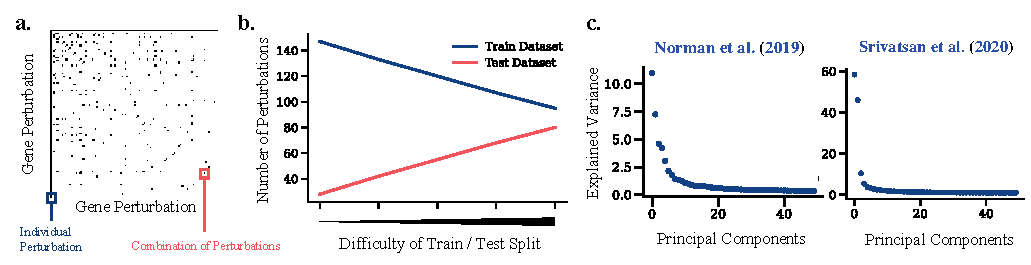
\includegraphics[width=.9\textwidth]{figures/fig_datasets_splits_processing.pdf}
    \caption{\textbf{a.} The indicator matrix of all individual perturbations as well as those perturbation pairs available in combination (black) in the dataset by \citet{norman2019exploring}. \textbf{b.} Size of the different train/test splits of the dataset by \citet{norman2019exploring}. The train set contains all single perturbations as well as a decreasing number of combinations with increasing difficulty of the data split. For more details, see \cref{app:datasplits}.}
    \label{fig:datasets_processing}
\end{figure}

\subsection{\citet{norman2019exploring}} 
\label{app:dataset_norman}

\looseness -1 Genetic interactions and their joint expression give rise to an inconceivable organismal complexity and uncountable many diverse phenotypes and behaviors.
Constructing a systematic genetic interaction map is crucial for a better understanding of cellular mechanisms in health and disease.
Thus, \citet{norman2019exploring} conducted \acrlong{sc}, pooled transcriptional profiling of \acrshort{CRISPR}-mediated perturbations to link genetic perturbation to its transcriptional consequences using the Perturb-seq technology \citep{dixit2016perturb, adamson2016multiplexed}.
The dataset consists of individual perturbations as well as joint overexpression of different genes, allowing us to study the phenotypic consequences of perturbing a pair of genes alone or in combination. The indicator matrix of all individual perturbations as well as those pairs available in combination can be found in \cref{fig:datasets_processing}a.

\paragraph{Data preprocessing.}
\looseness -1 The dataset is available for download in the \acrshort{GEO} database under accession number \href{https://www.ncbi.nlm.nih.gov/geo/query/acc.cgi?acc=GSE133344}{GSE133344}.
For data quality control and preprocessing, we follow the analysis of \citet{lotfollahi2021compositional}.
We discarded those genetic perturbations with less than $250$ cells, resulting in a dataset with $92$ individual perturbations and $84$ perturbations in combination.
This further included, the exclusion of particular subsets of control cells with in total of $98,419$ remaining, data normalization, log-transformation, and selection of $1,500$ \acrshortpl{HVG} using \texttt{scanpy} \citep{wolf2018scanpy}.

\paragraph{Feature selection.}
Similar to \cref{app:dataset_srivatsan}, for evaluation we select the top $50$ marker genes, i.e., those genes most strongly affected by the particular genetic perturbation.

\paragraph{Data splits.} \label{app:datasplits}
For the evaluation conducted in \cref{cha:condot}, we create different train/test dataset splits of increasing difficulty by following \citet{lotfollahi2021compositional}.
The train splits hereby always contain all $92$ individual perturbations as well as varying numbers of combinations. The easiest train split contains 55 perturbations, while the test set only carries 28 combinations that are unknown in the evaluation. Consecutive splits get increasingly harder, comprising 42, 29, 16, and 4 combinations in the train set (besides all single perturbations) and 41, 54, 67, and 79 combinations in the test set, respectively (see \cref{fig:datasets_processing}b).

\subsection{\citet{moon2019visualizing}}
\label{app:dataset_moon}

Developmental processes in biology involve tissue and organ development, body axis formation, cell division, and cell differentiation, e.g., the development of stem cells into functional cell types.
An example of such a process is the differentiation of \acrshortpl{ESC} into hematopoietic, cardiac, neural, pancreatic, hepatocytic, and germ lineages.
This development can be approximated \textit{in vitro} using \acrlongpl{EB} \citep{martin1975differentiation}, three-dimensional aggregates of pluripotent stem cells, including \acrshortpl{ESC} \citep{shamblott2009derivation}.
Recently, \citet{moon2019visualizing} conducted a \acrshort{sc}\acrshort{RNAseq} analysis to unveil the developmental trajectories, as well as cellular and molecular identities through which early lineage precursors emerge from human \acrshortpl{ESC}.
The dataset is available via \href{https://data.mendeley.com/datasets/v6n743h5ng}{Mendeley Data (V6N743H5NG)}\footnote{Dataset available via \url{https://data.mendeley.com/datasets/v6n743h5ng}.}.
In the following, we describe the preprocessing of the raw \acrshort{sc}\acrshort{RNAseq} data as well as the lineage branch analysis extracting the functional cell types emerging in this developmental process.

\paragraph{Data preprocessing.}
To preprocess the data, we follow the analysis of \citet{moon2019visualizing} as well as \citet{luecken2019current}. \citet{moon2019visualizing} originally measure  approximately $31,000$ cells over a 27 days differentiation time course, comprising gene expression matrices and barcodes, i.e., \acrshort{DNA} tags used to identify reads originating from the same cell. The measured cells are then filtered in a quality control stage, their gene expression levels normalized and further processed in a feature selection step, where only highly-differentiated genes are selected.
After quality control, the dataset consists of $15,150$ cells and $17,945$ genes.

\paragraph{Feature selection.}
We extract $4,000$ \acrshortpl{HVG} using the 10X genomics preprocessing software \texttt{Cell Ranger} \citep{zheng2017massively} to further reduce the dimensionality of the dataset and include only the most informative genes.
Given the resulting data matrix with $15,150$ cells and $4,000$ genes across 5 different time points, we compute a corresponding low-dimensional embedding using \acrshort{PCA}. We use the first 20 or 30 PCs for predicting population dynamics in \cref{cha:neural_pde} and \ref{cha:neural_sde}.
This is in alignment with previous analysis of developmental trajectories, which use 5 \citep{tong2020trajectorynet} and 30 PCs \citep{schiebinger2019optimal}, respectively.

\paragraph{Lineage branch analysis.}
Besides evaluating how well methods presented in this thesis resemble the spatiotemporal dynamics, we analyze their ability to capture biological heterogeneity.
Serving as an \emph{in vitro} model of early embryogenesis, \acrshort{EB} differentiation captures the development of \acrshortpl{ESC} into the mesoderm, endoderm, neuroectoderm, neural crest, and others.
Using an initial $k$-means clustering ($k=30$) and following \citet[Fig. 6, Suppl. Note 4]{moon2019visualizing}, we compute lineage branch classes for all cells in a 10-dimensional embedding space using PHATE, a non-linear dimensionality reduction method capturing a denoised representation of both the local and global structure of a dataset.
Details of the annotation can be found in \citet{bunne2022proximal, bunne2022recovering}.

We then train a \acrshort{kNN} classifier ($k=5$) to infer the lineage branch class based on a 30-dimensional \acrshort{PCA} embedding of a cell (\acrshort{ESC}: 0, neural crest: 1, neuroectoderm: 2, endoderm: 3, mesoderm: 4, other: 5).
\cref{sec:jkonet_cell} and \ref{sec:gsbflow_cell} contain an analysis of the captured lineage branch heterogeneity of the predictions by computing the lineage branch class of each cell using the \acrshort{kNN} classifier.

\subsection{\citet{weinreb2020lineage}}
\label{app:dataset_weinreb}

\citet{weinreb2020lineage} study lineage tracing on transcriptional landscapes in hematopoiesis, the process of blood regeneration in bone marrow, in which multipotent progenitors give rise to red cells of the blood, as well as myeloid and lymphoid immune cell types.
In order to dissect how molecular differences among progenitor cells determine their ability to generate mature cell types, it is crucial to understand the hierarchy of fate decisions connecting stem and progenitor cells through time.
Directly linking whole-transcriptome descriptions of cells to their future fate is challenging, however, as \acrlong{sc} \acrshort{RNAseq} technologies are destructive (see \cref{sec:tech_background}). 
\citet{weinreb2020lineage} therefore clonally tag cells with \acrshort{DNA} barcodes that can be read using sc\acrshort{RNAseq} and enable tracing cellular identities through time.
The resulting dataset consists of three snapshots taken on days 2, 4, and 6, respectively. While at day 2 most cells are undifferentiated, at later time points cells have developed into neutrophils, monocytes, megakaryocytes, mast cells, lymphoid precursors, erythrocytes, basophils, eosinophils, etc.

\paragraph{Data preprocessing.}
The dataset used in \cref{cha:cellot} and \cref{sec:sbalign} is available for download in the \acrshort{GEO} database under accession number \href{https://www.ncbi.nlm.nih.gov/geo/query/acc.cgi?acc=GSE140802}{GSE140802}.
For data quality control and preprocessing, we follow the analysis of \citet{lotfollahi2021compositional}, resulting in a dataset containing $130,861$ cells.
After processing, each observation records the level of expression of $1,622$ different \acrshortpl{HVG} as well as the following meta information per cell:
\begin{itemize}
    \item a \texttt{timestamp}, expressed in days and taking values in \{2, 4, 6\},
    \item a \texttt{barcode}, which is a short \acrshort{DNA} sequence that allows tracing the identity of cells and their lineage using \acrlong{sc} sequencing readouts,
    \item an additional \texttt{annotation}, which describes the current differentiation fate of the cell.
\end{itemize}

For experiments conducted in \cref{sec:sbalign_cell}, we only retain cells with barcodes that appear both on days 2 and 4, taking care of excluding cells that are already differentiated on day 2.
We construct matchings by pairing cells measured at two different times but which share the barcode. 
Additionally, we filter cells to make sure that no one appears in more than one pair.

\paragraph{Feature selection.}
To reduce the dimensionality of these data points, we perform a \acrshort{PCA} projection down to 50 components.

\subsection{Other Datasets}
\label{app:dataset_other}

Preprocessing for the lupus patients~\citep{kang2018multiplexed} and cross-species dataset~\citep{hagai2018gene} were inherited from~\citet{rybakov2020learning} 
and \citet{lotfollahi2019scgen}, and we would like to thank the authors for hosting this dataset.
Lastly, the preprocessing of the glioblastoma patient dataset \citep{zhao2021deconvolution} was adapted from \citet{peidli2022scperturb}.
The preprocessed datasets are available for download\textsuperscript{\ref{fnt:dataset_download}}. Similarly, for the dataset by \citet{schiebinger2019optimal}, the processed dataset is hosted by the authors\footnote{Dataset available via \url{https://broadinstitute.github.io/wot/tutorial/}.}.

\section{Evaluation Metrics} \label{app:evaluation_metrics}

\looseness -1 Since we lack access to the ground truth pair of perturbed and unperturbed observations on the single cell level, we consider evaluation metrics on the level of the distribution of real and predicted perturbation states to analyze the effectiveness of the approaches presented in this thesis.

\paragraph{Average- and Correlation-based distance.} 
Common evaluation metrics in \acrlong{sc} biology rely on averages and correlation analysis. $\ell_2$ feature means thereby refers to the $\ell_2$-distance between means of the observed and predicted distributions. Similarly, $r_2$ feature means refers to the correlation of the means of the observed and predicted distributions.
However, metrics based only on feature means can be insensitive in settings where crucial heterogeneity is not captured. Consider, for example, a target distribution with multiple modes. These metrics will favorably evaluate a uni-modal predicted distribution that simply models the mean of this multi-modal distribution. To this end, we include a distributional distance sensitive to this type of behavior by measuring differences in the properties of higher moments, i.e., the maximum mean discrepancy.
We thus also report results based on several distributional metrics:

\paragraph{Wasserstein distance.}
We measure accuracy of the predicted target population $\hat{\nu}$ to the observed target population $\nu$ using the entropy-regularized Wasserstein distance \citep{cuturi2013sinkhorn} provided in the \texttt{OTT} library \citep{cuturi2022optimal} introduced in \cref{sec:background_kantorovich} and defined in \eqref{eq:ot-reg}.

\paragraph{Maximum mean discrepancy.}
Kernel maximum mean discrepancy~\citep{gretton2012kernel} is another metric to measure distances between distributions, i.e., for our purpose between the predicted target population $\hat{\nu}$ to the observed target population $\nu$.
Given two random variables $x$ and $y$ with distributions $\hat{\nu}$ and $\nu$, and a kernel function $\omega$, \citet{gretton2012kernel} define the squared \acrshort{MMD} as:
\begin{equation*}
    \text{MMD}(\hat{\nu},\nu; \omega) = \mathbb{E}_{x,x^\prime}[\omega(x, x^\prime)] + \mathbb{E}_{y,y^\prime}[\omega(y, y^\prime)] - 2\mathbb{E}_{x,y}[\omega(x, y)].
\end{equation*}
We report an unbiased estimate of $\text{MMD}(\hat{\nu},\nu)$, in which the expectations are evaluated by averages over the population particles in each set. We utilize the RBF kernel, and as is usually done, report the \acrshort{MMD} as an average over several length scales, i.e., \texttt{np.logspace(1, -3)}.

\paragraph{Perturbation signatures.}
A common method to quantify the effect of a perturbation on a population is to compute its \acrlong{PS} \citep[PS]{stathias2018drug}, computed via the difference in means between the distribution of perturbed states and control states of each feature, e.g., here individual genes. $\ell_2$(\acrshort{PS}) then refers to the $\ell_2$-distance between the \acrlongpl{PS} computed on the observed and predicted distributions, $\nu$ and $\hat{\nu}$. As before, let $\mu$ be the set of observed unperturbed population particles, $\nu$ the set of observed perturbed particles, as well as $\hat{\nu}$ the predicted perturbed state of population $\mu$. The $\ell_2$(PS) is then defined as
\begin{equation*}
    \text{PS}(\nu, \mu) = \frac{1}{m}\sum_{y_i \in \nu}{y_i} - \frac{1}{n}\sum_{x_i \in \mu}{x_i},
\end{equation*}
where $n$ is the size of the unperturbed and $m$ of the perturbed population.
We report the $\ell_2$ distance between the observed signature $\text{PS}(\nu, \mu)$ and the predicted signature $\text{PS}(\hat{\nu}, \mu)$, which is equivalent to simply computing the difference in the means between the observed and predicted distributions.


\numberwithin{equation}{section}		% for numbering  in the appendix
\numberwithin{lemma}{section}		% for numbering  in the appendix
\numberwithin{proposition}{section}		% for numbering  in the appendix
\numberwithin{theorem}{section}		% for numbering in the appendix

%----------------------------------------------------------------------
%%% PROOF OF BURES-WASSERSTEIN MECHANICS
%----------------------------------------------------------------------
\section{Proof of \cref{thm:gsbtobb}}
\label{app:gsbtobb}


It is known that, for \acrshortpl{SB}, the optimal solution can be searched within the class of stochastic processes \citep{leonard2013survey}
\begin{equation}
\label{eq:holddd}
X_t \sim \Pmargin: \quad\dd X_t =  (\driftf(X_t) + \vectalt(X_t) )\dt + \volat \dWiener[\ctime].
\end{equation}
The Fokker-Planck equation for the \acrshort{SDE} \eqref{eq:holddd} is
\begin{align}
\label{eq:FK}
\del_t \measure = - \Div \parens*{  \measure(  \driftf +\vectalt  ) } + \frac{\volatsq[\ctime]}{2}\Laplace \measure.
\end{align}
A simple application of the Girsanov theorem then shows, up to a constant, 
\begin{align}
\label{eq:KLobj}
\KL(\Pmargin \| \refsde) = \exof*{ \int_0^\horizon\frac{\norm{\vectalt}^2}{2\volatsq[\ctime]}   \dt}.
\end{align}
Using a change of variable $\vect = \vectalt - \frac{\volatsq[\ctime]}{2}\nabla\log\measure$, we see that \eqref{eq:FK} is equivalent to
\begin{equation}
\del_t \measure = - \Div \parens*{  \measure(  \driftf +\vect  ) }.
\end{equation}
On the other hand, since $\norm{\vectalt}^2 = \norm{\vect}^2 + \frac{\volat^4}{4}\norm*{\nabla\log\measure}^2 + 2 \inner*{\vect}{ \frac{\volatsq[\ctime]}{2}\nabla\log\measure}$, the integrand in the objective of \eqref{eq:KLobj} becomes 
\begin{align}
 \mathbb{E}\Bigg[\int_0^\horizon  \frac{\norm{\vect}^2}{2\volatsq[\ctime]} + \frac{\volatsq[\ctime]}{8} \norm{\nabla \log \measure}^2  + \frac{1}{2} \inner{\vect}{\nabla \log\measure} \dt\Bigg].
\end{align}


Letting $H(\measure) \defeq \int \measure\log\measure$ be the entropy, we have
\begin{align*}
H(\measure[\horizon]) - H(\measure[0]) &= \int_0^\horizon \del_t H(\measure) \dt \\
&= \int_0^\horizon  \int   (1+ \log\measure) \del_t\measure \drm \point \dt  \\
&= \int_0^\horizon  \int   (1+ \log\measure) \cdot \parens*{ - \Div \parens*{ \measure(\driftf+\vect) }  } \drm \point \dt  \quad\quad \text{by \eqref{eq:FK}}\\
&= \int_0^\horizon  \int   \measure \inner{\nabla\log\measure}{ \driftf+\vect} \drm \point \dt 
\end{align*}
by integration by parts for the divergence operator. Therefore,
\begin{align}
\exof*{\int_0^\horizon  \inner{\nabla\log\measure}{ \vect}  \dt } = H(\measure[\horizon]) - H(\measure[0])-\exof*{\int_0^\horizon  \inner{\nabla\log\measure}{ \driftf}  \dt }
\end{align} 
which concludes the proof.\qed



%----------------------------------------------------------------------
%%% PROOF OF BURES-WASSERSTEIN MECHANICS
%----------------------------------------------------------------------
\section{The Bures-Wasserstein Geometry of Gaussian SBs}
\label{app:mechanics}

\subsection{Review of Bures-Wasserstein Geometry}

\label{app:reviewBW}

Recall that the \emph{metric tensor} $\innerBW[\cdot][\cdot][\Sigma]$ in the \emph{Bures-Wasserstein geometry} \citep{takatsu2010wasserstein} is defined in terms of the Lyapunov operator: 
\begin{align}
\label{eq:BW-tensor}
\forall\ U, V\in \tspace, \quad \innerBW[U][V][\Sigma] \defeq \tr\lyap[\Sigma][U]\Sigma\lyap[\Sigma][V] = \frac{1}{2}\tr \lyap[\Sigma][U]V.
\end{align}The corresponding Bures-Wasserstein norm is induced via $\normBWsq[U][\Sigma] \defeq \innerBW[U][U][\Sigma]$.
Another important operator is the Bures-Wasserstein \emph{gradient}: For any function $F \from \SPD \to \R$, 
\begin{equation}
\label{eq:gradBW-def}
\tspace\ni \gradBW F(\Sigma) \defeq 2 \parens*{ \nabla F(\Sigma)\Sigma + \Sigma \nabla F(\Sigma)^T }
\end{equation}where $\nabla$ is the usual Euclidean gradient of $F$, viewed as a function from $\R^{\vdim\times\vdim}$ to $\R$. Note that
\begin{align}
\lyap[\Sigma][\gradBW F(\Sigma)] &= 2 \lyap[\Sigma][\nabla F(\Sigma)\Sigma + \Sigma\nabla F(\Sigma)] \\
&= 2 \nabla F(\Sigma)
\end{align}by definition of the Lyapunov operator. In other words,
\begin{align}
\label{eq:gradBW-lyapinv}
\gradBW F(\Sigma) = \lyapinv.
\end{align}


Lastly, we recall the Bures-Wasserstein \emph{acceleration} of a curve $\Sigcurve: [0,\horizon] \to \SPD$, which we denote by $\nabla_{\ssstyle\dSigcurve}\dSigcurve$:\footnote{More formally, $\nabla_{\ssstyle\dSigcurve}\dSigcurve$ is the Bures-Wasserstein covariant derivative of $\dSigcurve$ in the direction of $\dSigcurve$.}

\begin{align}
\label{eq:coderBW}
\coder = \ddSigcurve -  \parens*{  \lyap \dSigcurve + \dSigcurve\lyap } + \parens*{ \Sigcurve \parens*{\lyap}^2 + \parens*{\lyap}^2 \Sigcurve}.
\end{align}





\subsection{Proof of \cref{thm:mechanics}}
\label{app:proofmechanics}


For convenience, we restate \cref{thm:mechanics} in full below: 
\mechanics*


The proof consists of verifying the Euler-Lagrange equation \eqref{eq:el-bw} for the curve \eqref{eq:solMain}.

\subsubsection{Verifying the Euler-Lagrange Equation \eqref{eq:el-bw}}
\label{sec:verifyEL}
We begin by noting that the boundary conditions in \eqref{eq:el-bw} hold for the curve in \eqref{eq:solMain}. 


We now compute the two sides of \eqref{eq:el-bw} separately:

\paragraph{The right-hand side of \eqref{eq:el-bw}: $-\gradBW\penergyBW$.}
~Since $\nabla \penergyBW = -\nabla \parens*{\tr \frac{\sdev^4}{8} \Sigcurveinv} =  \frac{\sdev^4}{8} \Sigcurveinv\cdot \Sigcurveinv$, we see from \eqref{eq:gradBW-def} that the negative Bures-Wasserstein gradient of $\penergyBW$ is
\begin{align}
\nn
-\gradBW \penergyBW &= -2\parens*{\frac{\sdev^4}{8} \Sigcurveinv\cdot \Sigcurveinv \cdot \Sigcurve + \Sigcurve\cdot \frac{\sdev^4}{8} \Sigcurveinv\cdot \Sigcurveinv } \\
\label{eq:gradBWU}
&= -\frac{\sdev^4}{2} \Sigcurveinv.
\end{align}


\paragraph{The left-hand side of \eqref{eq:el-bw}: $\coder$.}
~Computing $\coder$ is significantly trickier than $-\gradBW\penergyBW$. The central piece of the proof is the following technical lemma:
\begin{lemma}
\label{lem:lyap}
Define the matrix $\Ht$ to be:
\begin{equation}
\label{eq:Ht}
\Ht \defeq \ctime\Sigma\prime + \ctimebar \C - \ctimebar\Sigma - \ctime\C^T  + \frac{\sdev^2}{2}(\ctimebar-\ctime)\eye.
\end{equation}Then $\lyap = \Ht^T  \Sigcurveinv$. In other words, $\Ht^T  \Sigcurveinv$ is symmetric and solves the Lyapunov equation:
\begin{equation}
  A: \quad  A\Sigcurve + \Sigcurve A= \dSigcurve.
\end{equation}
Moreover, $\Ht$ satisfies the following identity:
\begin{equation}
\label{eq:ht-id}
\dHt - \Sigcurveinv \Ht^2 =- \frac{\sdev^4}{4} \Sigcurveinv.
\end{equation}

\end{lemma}

Before commencing the proof of \cref{lem:lyap}, let us show how it readily leads us to \eqref{eq:el-bw}.

Recall the definition of $\coder$ in \eqref{eq:coderBW}. First, note that, by \eqref{eq:solMain} and \eqref{eq:Ht},
\begin{align}
\label{eq:ddot}
\frac{1}{2}\ddSigcurve &=   \Sigma+\Sigma\prime -  \parens*{  \C + \C^T + \sdev^2\eye }   \\
&=  \dHt.
\end{align}
On the other hand, \cref{lem:lyap} entails that
\begin{align}
\nn
\Sigcurve \parens*{\lyap}^2 + \parens*{\lyap}^2 \Sigcurve &= \Sigcurve \lyap \cdot \lyap + \lyap \cdot \lyap\Sigcurve \\
\nn
 &= \Sigcurve \Sigcurveinv \Ht \cdot \lyap + \lyap \cdot \Ht^T  \Sigcurveinv \Sigcurve \\
 \label{eq:holdBW}
 &= \Ht \lyap + \lyap \Ht^T .
\end{align}
By noting, again from \cref{lem:lyap},
\begin{align}
\nn
\dSigcurve &= \Ht^T  \Sigcurveinv \cdot \Sigcurve + \Sigcurve \cdot \Sigcurveinv\Ht \\
\label{eq:HtHtt}
&= \Ht + \Ht^T ,
\end{align}
we thus get
\begin{align}\nn
 \Sigcurve \parens*{\lyap}^2 &+ \parens*{\lyap}^2 \Sigcurve- \parens*{  \lyap \dSigcurve + \dSigcurve\lyap } \\
 &= \parens*{\Ht - \dSigcurve} \lyap + \lyap \parens*{\Ht^T  - \dSigcurve} \\
 \nn
 &= - \parens*{ \Ht^T \lyap + \lyap \Ht  }
\end{align}by \eqref{eq:HtHtt}. But $\Ht^T \lyap  = \Ht^T  \cdot \Sigcurveinv \Ht =\Sigcurveinv \Ht^2$ by symmetry of $\Ht^T  \Sigcurveinv$ and, similarly, we have $\lyap\Ht =  \Sigcurveinv \Ht^2$. As a result, \eqref{eq:coderBW} reduces to
\begin{align}
\label{eq:holdBW1}
\coder &= 2\dHt - 2 \Sigcurveinv\Ht^2.
\end{align}In lieu of \eqref{eq:el-bw}, \eqref{eq:gradBWU}, and \eqref{eq:holdBW1}, the proof of \eqref{eq:LagBW} can thus be reduced to showing
\begin{align}
2\dHt -  2\Sigcurveinv\Ht^2 = -\frac{\sdev^4}{2} \Sigcurveinv
\end{align}which is exactly \eqref{eq:ht-id}.



\begin{proof}[Proof of \cref{lem:lyap}] 
We now prove \cref{lem:lyap}. We begin by proving some useful identities that will inspire our proof for the general \acrshortpl{GSB} in \cref{sec:results_gsbflow}.

\paragraph{Useful identities.}
~First, note that the definition of $\C$ immediately implies $\C \Sigma = \Sigma \C^T $. In addition, we have
\begin{align}
\nn
\C^{-1} \Sigma &= 2\parens*{ \Sigma^{\frac{1}{2}} \D  \Sigma^{-\frac{1}{2}} - \sdev^2\eye }^{-1} \Sigma \\
\nn
&= 2 \parens*{ \Sigma^{-\frac{1}{2}} \D  \Sigma^{-\frac{1}{2}} - \sdev^2\Sigma^{-1} }^{-1} \\
\label{eq:Csym}
&= \Sigma \C^{-T }.
\end{align}
Recall from \citep{janati2020entropic} that $\C$ solves the following matrix equation:
\begin{align}
\label{eq:C}
\C^2 + \sdev^2\C =  \Sigma\Sigma\prime.
\end{align}
We therefore have
\begin{align*}
\C &= \C^{-1} \Sigma\Sigma\prime - \sdev^2\eye, \\
\C^T  &= \Sigma\prime\Sigma\C^{-T } - \sdev^2\eye,
\end{align*}which, together with \eqref{eq:Csym}, implies
\begin{align}
\nn
\C^T  \Sigma\prime &= \Sigma\prime\Sigma \C^{-T }\Sigma\prime-\sdev^2\Sigma\prime  \\
\nn
&=\Sigma\prime \C^{-1}\Sigma \Sigma\prime-\sdev^2\Sigma\prime   \\
\label{eq:Ctsym}
&= \Sigma\prime \C.
\end{align}


Now, set $\Ht = \Pt - \Qt^T  + \frac{\sdev^2}{2}(\ctimebar-\ctime)\eye$ where
\begin{align}
\Pt \defeq \ctime \Sigma\prime + \ctimebar \C, \quad \Qt \defeq \ctimebar \Sigma + \ctime \C.
\end{align}
Note that, by \eqref{eq:Ctsym}, 
\begin{align}
\nn
\Sigma\prime\Pt^{-1}  &= \parens*{ \Pt\Sigma\prime^{-1} }^{-1} \\
\nn
&= \parens*{\ctime\eye + \ctimebar  \C \Sigma\prime^{-1} }^{-1} \\
\nn
&=  \parens*{\ctime\eye + \ctimebar \Sigma\prime^{-1} \C^T   }^{-1} \\
\nn
&= \parens*{ \Sigma\prime^{-1} \Pt^T   }^{-1} \\
\label{eq:Ptsym}
&= \Pt^{-T }\Sigma\prime.
\end{align}A similar calculation leading to \eqref{eq:Ptsym} shows
\begin{align}
\label{eq:Qtsym}
\Qt^{-1} \Sigma = \Sigma\Qt^{-T }.
\end{align}

\paragraph{Proof of symmetry of $\Ht^T \Sigcurveinv$.}
~We get, by \eqref{eq:C} and \eqref{eq:Ctsym},

\begin{align}
\nn
\Pt^2 + \sdev^2\ctimebar\Pt &= t^2 \Sigma\prime^2 + \ctimebar^2\C^2 + \ctime\ctimebar\parens*{ \Sigma\prime\C + \C\Sigma\prime } + \sdev^2 \ctime\ctimebar \Sigma\prime + \sdev^2\ctimebar^2 \C \\
\nn
&= t^2 \Sigma\prime^2 + \ctimebar^2 \parens*{ \C^2 + \sdev^2\C } + \ctime\ctimebar\parens*{ \C^T \Sigma\prime + \C\Sigma\prime } + \sdev^2 \ctime\ctimebar \Sigma\prime\\
\label{eq:Pteq}
&= t^2 \Sigma\prime^2 + \ctimebar^2 \Sigma\Sigma\prime + \ctime\ctimebar\parens*{ \C^T  + \C + \sdev^2\eye}\Sigma\prime = \Sigcurve\Sigma\prime.
\end{align}

It then follows from \eqref{eq:Pteq} that

\begin{align}
\label{eq:Pt2}
\Pt &=  \Sigcurve\Sigma\prime\Pt^{-1} - \sdev^2 \ctimebar\eye, \\
\label{eq:Ptt2}
\Pt^T  &=  \Pt^{-T } \Sigma\prime\Sigcurve - \sdev^2\ctimebar\eye.
\end{align}

As a result, we get, by \eqref{eq:Ptsym} and \eqref{eq:Pt2}-\eqref{eq:Ptt2},

\begin{align}
\nn
\Sigcurveinv \Pt &= \Sigma\prime\Pt^{-1} - \sdev^2\ctimebar\Sigcurveinv \\
\nn
&= \Pt^{-T }\Sigma\prime - \sdev^2\ctimebar\Sigcurveinv \\
\label{eq:PtSig}
&= \Pt^T \Sigcurve^{-1}.
\end{align}

In exactly the same vein, we have

\begin{align}
\label{eq:Qteq}
\Qt^2 + \sdev^2 \ctime\Qt = \Sigma\Sigcurve
\end{align}

as well as

\begin{align}
\label{eq:QtSig}
\Sigcurveinv\Qt^T  = \Qt \Sigcurveinv.
\end{align}The symmetry of $\Ht^T \Sigcurveinv$ is then an immediate consequence of \eqref{eq:PtSig} and \eqref{eq:QtSig}. In addition, we have
\begin{align}
\nn
\dSigcurve &= 2\ctime\Sigma\prime - 2 \ctimebar\Sigma + (\ctimebar-\ctime)\parens*{   \C +\C^T   + \sdev^2\eye } \\
\label{eq:HtHtt2}
&=  \Ht + \Ht^T .
\end{align}
Combining the symmetry of $\Ht^T \Sigcurveinv$ and \eqref{eq:HtHtt2}, we see that
\begin{align}
\nn
\Ht^T \Sigcurveinv \cdot \Sigcurve + \Sigcurve \cdot \Sigcurveinv \Ht = \Ht+\Ht^T  = \dSigcurve,
\end{align}
i.e., $\lyap = \Ht^T \Sigcurveinv$.



\paragraph{Proof of \eqref{eq:ht-id}.}

We next compute
\begin{align}
\nn
\Pt \Qt^T  &= \parens*{\ctime \Sigma\prime + \ctimebar \C}\parens*{\ctimebar \Sigma + \ctime \C^T } \\
\nn
&= \ctime\ctimebar\Sigma\prime\Sigma + \ctime^2\Sigma\prime\C^T  + \ctimebar^2\C\Sigma + \ctime\ctimebar\C\C^T  \\
\nn
&= \ctimebar^2\Sigma \C^T  + \ctime^2\Sigma\prime\C^T + \ctime\ctimebar \parens*{ \C^{T  2}+ \sdev^2\C^T  }+ \ctime\ctimebar  \C\C^T 
\\
\label{eq:PtQtt}
&= \Sigcurve\C^T 
\end{align}
where we have used \eqref{eq:Csym} in the third equality of \eqref{eq:PtQtt}. A similar computation further shows 
\begin{align}
\label{eq:QttPt}
\Qt^T \Pt = \Sigcurve\C.
\end{align}

We thus get, by combining \eqref{eq:Pteq} \eqref{eq:Qteq}
\begin{align}
\nn
\Ht^2 &= \Pt^2 -\Pt \Qt^T  + \frac{\sdev^2}{2}(\ctimebar-\ctime) \Pt -\Qt^T  \Pt + \Qt^{T 2} - \frac{\sdev^2}{2}(\ctimebar-\ctime)\Qt^T  +  \frac{\sdev^2}{2}(\ctimebar-\ctime)\Pt \\
	& \enspace\enspace -  \frac{\sdev^2}{2}(\ctimebar-\ctime)\Qt^T  + \frac{\sdev^4}{4}(\ctimebar-\ctime)^2\eye \\
\nn
&= \Pt^2 + \sdev^2(\ctimebar-\ctime)\Pt + \Qt^{T 2} - \sdev^2(\ctimebar-\ctime)\Qt^T  - \parens*{ \Pt\Qt^T  + \Qt^T  \Pt }  + \frac{\sdev^4}{4}(\ctimebar-\ctime)^2\eye\\
\nn
&= \Sigcurve\Sigma\prime - \sdev^2\ctime\Pt + \Sigcurve \Sigma - \sdev^2 \ctimebar\Qt^T  - \parens*{  \Sigcurve \C^T  + \Sigcurve \C }  + \frac{\sdev^4}{4}(\ctimebar-\ctime)^2\eye - \sdev^2 \Sigcurve + \sdev^2\Sigcurve\\
\nn
&= \Sigcurve\parens*{  \Sigma + \Sigma\prime - \parens*{\C + \C^T  + \sdev^2\eye }} + \sdev^2 \parens*{\Sigcurve -  \ctime\Pt - \ctimebar\Qt^T  }+ \frac{\sdev^4}{4}(\ctimebar-\ctime)^2\eye  \\
\nn 
&= \Sigcurve \dHt + \sdev^2 \cdot\ctime\ctimebar\sdev^2 \eye +  \frac{\sdev^4}{4}(\ctimebar-\ctime)^2\eye \\
\label{eq:holdBW3}
&= \Sigcurve \dHt + \frac{\sdev^4}{4}\eye
\end{align}
where the third equality follows from \eqref{eq:Pteq}, \eqref{eq:Qteq}, and \eqref{eq:PtQtt}-\eqref{eq:QttPt}, and the fifth equality follows from \eqref{eq:Ht}. Multiplying both sides of \eqref{eq:holdBW3} by $\Sigcurveinv$ from the right yields the desired \eqref{eq:ht-id}. 
\end{proof}


\subsubsection{Equivalence between \eqref{eq:GaussianSBWiener} and \eqref{eq:LagBW}}

We first note that, by \eqref{eq:BW-tensor} and \cref{lem:lyap},
\begin{align}
\nn
\kenergyBW &= \frac{1}{2}\tr \lyap \Sigmasol \lyap \\
\nn
&= \frac{1}{2}\tr \Ht^T  \Sigmasolinv \cdot \Sigmasol \cdot \Sigmasolinv \Ht \\
&= \frac{1}{2} \tr \Ht^T \Sigmasolinv\Ht,
\end{align}and therefore the integrand in \eqref{eq:LagBW} is equal to
\begin{align}
\label{eq:holdBW2}
\tr \parens*{   \frac{1}{2} \Ht^T \Sigmasolinv\Ht + \frac{\sdev^4}{8} \Sigcurveinv}.
\end{align}


To proveed, we will need another formulation of \eqref{eq:GaussianSBWiener}, which is \citep{chen2016relation, gentil2017analogy} specialized to our case: 
\begin{lemma}\label{lem:EntOT}
Let $\Ncal_0 \defeq \Ncal(0,\Sigma)$ and $\Ncal_\horizon \defeq \Ncal(0,\Sigma\prime)$. Then \eqref{eq:GaussianSBWiener} is equivalent to
\begin{align}
\label{eq:LagMeasure}
\min_{\ssstyle\substack{{\measure[0] = \Ninit, \measure[\horizon] = \Nend}}} \int_{0}^\horizon  \exof*{\frac{1}{2} \norm{\vecsol}^2 + \frac{\sdev^4}{8} \norm{ \nabla \log \measure }^2} \dt
\end{align}where the minimization is taken over all pairs $(\measure, \vecsol)$ such that $\Phi_\ctime:\R^\vdim\to\R$ are differentiable functions and the continuity equation holds:
\begin{equation}
\label{eq:ConeqApp}
\pt\measure = - \Div(\measure \vecsol).
\end{equation}
\end{lemma}

We will also need the \emph{Jacobi formula}: Let $A(\ctime) \from \R^+ \to \R^{\vdim\times\vdim} $ be a differentiable matrix-valued function. Then
\begin{align}
\label{eq:jacobi}
\ddt \det A(\ctime) = \det A(\ctime) \cdot \tr A^{-1}(\ctime) \cdot \ddt A(\ctime).
\end{align}

We are now ready to finish the proof of \cref{thm:mechanics}. By \citet{leonard2013survey}, the optimal curve for \eqref{eq:LagMeasure} is Gaussian with zero mean. We denote by $\Sigmasol$ the covariance of the solution at time $\ctime$. By \eqref{eq:jacobi}, we have
\begin{align}
\nn
\pt\measure(\point) &= \pt \parens*{ \nconst (\det\Sigmasol)^{-\frac{1}{2}} \exp\parens*{ -\frac{1}{2}\point^T  \Sigmasolinv\point   }}  \\
\nn
&=   \nconst \parens*{-\frac{1}{2} (\det\Sigmasol)^{-\frac{3}{2}}}  
\cdot\det\Sigmasol\cdot \tr \Sigmasolinv \dSigmasol \exp\parens*{ -\frac{1}{2}\point^T  \Sigmasolinv\point   } \\
\nn
&\hspace{10mm}+ \nconst (\det\Sigmasol)^{-\frac{1}{2}} \exp\parens*{ -\frac{1}{2}\point^T  \Sigmasolinv\point   } \cdot \parens*{\frac{1}{2} \point^T  \Sigmasolinv \dSigmasol \Sigmasolinv \point} \\
\label{eq:pt-m}
&= \measure(\point) \cdot \parens*{ \frac{1}{2} \point^T  \Sigmasolinv \dSigmasol \Sigmasolinv \point -\frac{1}{2}\tr \Sigmasolinv \dSigmasol }.
\end{align}


On the other hand, by the chain rule for the divergence, we have
\begin{align}
\label{eq:div-mv}
\Div(\measure \vecsol)  &=   \inner{\nabla\measure}{\vecsol}  + \measure \Laplace\potsol.
\end{align}
Since $\nabla \measure = \measure \parens*{ -\Sigmasolinv\point }$, the continuity equation \eqref{eq:ConeqApp} together with \eqref{eq:pt-m}-\eqref{eq:div-mv} implies that $\Sigmasol$ must satisfy
\begin{align}
\Laplace\potsol &= \frac{1}{2} \tr \Sigmasolinv \dSigmasol, \\
\inner{\Sigmasolinv\point}{\vecsol(\point)}  &= \frac{1}{2} \inner{\Sigmasolinv\point}{\dSigmasol\Sigmasolinv\point}, \quad \forall \point \in \R^\vdim.
\end{align}
In other words, the optimal vector field is of the form $\vecsol(\point) = \Ht^T \Sigmasolinv\point$ for some matrix $\Ht$ such that 
\begin{align}
\tr\Ht^T  \Sigmasolinv &= \frac{1}{2}\tr\dSigmasol\Sigmasolinv, \\
\tr \Sigmasolinv \Ht^T \Sigmasolinv \point\point^T  &=\frac{1}{2} \tr \Sigmasolinv \dSigmasol \Sigmasolinv \point\point^T , \quad \forall \point\in\R^\vdim.
\end{align}
Therefore, we see that
\begin{align}
\nn
\exof*{\norm{\vecsol}^2} &= \exof*{\tr \Ht^T \Sigmasolinv\point \point^T \Sigmasolinv \Ht} \\
\nn
&= \tr \Ht^T \Sigmasolinv \exof{\point\point^T } \Sigmasolinv \Ht \\
&= \tr \Ht^T \Sigmasolinv \Ht.
\end{align}
Furthermore, we have
\begin{align}
\nn
\exof*{ \norm{\nabla \log \measure}^2} &= \exof*{\tr \Sigmasolinv \point\point^T  \Sigmasolinv } \\
&= \tr \Sigmasolinv.
\end{align}
Finally, since the optimal vector field $\vecsol$ is a gradient field, we must have $\Ht^T  \Sigmasolinv = \Sigmasolinv\Ht$. Combing all the above, we see that \eqref{eq:LagMeasure} is equivalent to
\begin{align}
\label{eq:LagMeasureEquiv}
\min_{\ssstyle\substack{{\Sigcurve[0] = \Sigma, \Sigcurve[\horizon] = \Sigma\prime} \\ { \Ht^T \Sigcurveinv =  \Sigcurveinv\Ht }}} \int_{0}^\horizon  \tr\ \parens*{\frac{1}{2}\Ht^T \Sigcurveinv \Ht  + \frac{\sdev^4}{8} \Sigcurveinv} \dt
\end{align}which, in view of \eqref{eq:holdBW2}, is exactly the same as \eqref{eq:LagBW}.


\subsection{Some Interesting Consequences of \cref{thm:mechanics}}
\label{sec:interesting}

Here, we collect some interesting corollaries of \cref{thm:mechanics}, although they will not be used in the rest of the thesis.

\subsubsection{Conservation of Hamiltonian}
The first result concerns the \emph{Hamiltonian formulation} of the action minimization problem \eqref{eq:LagBW}. 
 
\NewDocumentCommand{\codiv}{ O{\dSigmasol} O{\dSigmasol} }{ \nabla_{\ssstyle #1}{#2} }
\newcommand{\hambase}{ \mathcal{H} }
\newcommand{\ham}[1][\Sigmasol]{ \hambase\parens*{#1} }

\begin{corollary}[Conservation of Hamiltonian]
Define the \textbf{Hamiltonian} associated with \eqref{eq:LagBW} to be
\begin{align}
\nn
\ham &\defeq \kenergyBW + \penergyBW \\
\label{eq:HamBW}
\tag{H}
&=  \tr  \parens*{\frac{1}{2} \Ht^T \Sigmasolinv\Ht - \frac{\sdev^4}{8} \Sigmasolinv}.
\end{align}Then the Hamiltonian is conserved along $\Sigmasol$: 
\begin{align}
\dot{\hambase} \equiv 0,  \text{ or, equivalently, }  \ham = \tr \parens*{\Sigma + \Sigma\prime - \D} \textup{ for all $\ctime$.}
\end{align}
\end{corollary}

The fact that the Hamiltonian, commonly interpreted as the \emph{total energy}, is conserved is a well-known fact in physics \citep{villani2009optimal} and directly follows from \cref{thm:mechanics}.

\subsubsection{Connection to Fisher Information}

The "potential energy" term $\penergyBW$ in \eqref{eq:LagBW} has an interesting origin: It is, up to a constant, the \emph{entropy production rate}, i.e., the \emph{Fisher information}.


\begin{lemma}\label{lem:Fisher}
Let $\measurebase \sim \Ncal(0,\covbase)$, and let $\entropy$ be the (negative) Shannon entropy of $\measurebase$. Then 
\begin{equation}
\label{eq:BW-U-Fisher}
\penergyBW = \frac{1}{2}\fisherBW %\frac{\sdev^4}{8} \tr \covbase^{-1} =  \frac{\sdev^4}{8} \tr \covbase^{-1}.
\end{equation}where 
\begin{equation}
\label{eq:BW-Fisher}
\fisherBW \defeq \frac{\sdev^4}{4} \normBWsq[\gradBW \entropy][\covbase].
\end{equation}
\end{lemma}
\begin{proof}
Recall that $\nabla \entropy= \nabla\parens*{ -\frac{1}{2} \log\det \covbase - \frac{\vdim}{2} \log 2\pi e }= -\frac{1}{2}  \covbase^{-1}$. Therefore, by \eqref{eq:BW-tensor} and \eqref{eq:gradBW-lyapinv},
\begin{align*}
\fisherBW &= \frac{\sdev^4}{4} \normBWsq[\gradBW \entropy][\covbase] \\
&= \frac{\sdev^4}{4}\innerBW[\gradBW \entropy][\gradBW \entropy][\covbase] \\
&= \frac{\sdev^4}{4} \tr \lyap[\covbase][\gradBW \entropy]\covbase\lyap[\covbase][\gradBW \entropy] \\
&= \frac{\sdev^4}{4} \tr \lyap[\covbase][\lyapinv[\covbase][2\nabla \entropy]]\covbase\lyap[\covbase][\lyapinv[\covbase][2\nabla \entropy]] \\
&= \frac{\sdev^4}{4} (-\covbase^{-1})\covbase(-\covbase^{-1})=\frac{\sdev^4}{4}\covbase^{-1}.
\end{align*}
\end{proof}

An infinite-dimensional version of \cref{lem:Fisher} for non-Gaussian measures is proved in \citet{chen2016relation, gentil2017analogy}; the connection to the Bures-Wasserstein geometry here seems to be new.

The specific form of the potential energy in \eqref{eq:BW-Fisher} has been shown to be intimately related to the \emph{gradient flow} of entropy:
\begin{align}
\dSigcurve = - \gradBW \entropy.
\end{align}

We refer the interested readers to \citep{gentil2020dynamical} for details.


\subsubsection{Solution of the Schr{\"o}dinger Systems}

For convenience, we restate the solutions of the Schr{\"o}dinger system introduced in \cref{sec:background_sb}, i.e., Equations \eqref{eq:sb_hb} and \eqref{eq:sb_optimality}.
Another way of solving a system of the form \eqref{eq:LagMeasure} is via the so-called forward \emph{Schr{\"o}dinger system} \citep{chen2021stochastic, leonard2013survey}:
\begin{align}
\label{eq:SchSys}
\left\{\begin{array}{lr}
\del_t \mu_t +\Div\parens*{  \mu_t\nabla \pot } = \frac{\sdev^2}{2}  \Laplace\mu_t \\
       \del_t \pot + \frac{\norm{ \nabla\pot}^2}{2} + \frac{\sdev^2}{2} \Laplace \pot = 0
        \end{array}\right..
\end{align}

By the various identities we prove in \cref{sec:verifyEL}, one can easily show that the solution to \eqref{eq:SchSys} is given by
\begin{align}
\pot(\point) = - \frac{\sdev^2}{4} \log\det\Sigmasol + \frac{\sdev^4}{4}  \int_{0}^t \tr \Sigmasolinv \dt + \frac{1}{2} \inner{\point}{\parens*{\Ht^T - \frac{\sdev^2}{2}\eye}\Sigmasolinv \point} + \const
\end{align}

This is in fact the same solution of the \emph{fluid mechanical} problem
\begin{align}
\min_{\ssstyle\substack{{\measure[0] = \Ninit, \measure[\horizon] = \Nend} \\ {\pt\measure +\Div(\measure \vecsol) =\Laplace \measure }}} \int_{0}^\horizon  \exof*{\frac{1}{2} \norm{\vecsol}^2 } \dt
\end{align}which is yet another equivalent formulation of \eqref{eq:GaussianSBWiener}.

There is also a backward Schr{\"o}dinger system:
\begin{align}
\left\{\begin{array}{lr}
-\del_t \mu_t + \Div\parens*{  \mu_t\nabla \rpot } =\frac{\sdev^2}{2}  \Laplace\mu_t  \\
      - \del_t \rpot + \frac{\norm{ \nabla\rpot}^2}{2} +\frac{\sdev^2}{2} \Laplace \rpot = 0
        \end{array}\right.,
\end{align}
whose solution is given by
\begin{align}
\rpot(\point) = - \frac{\sdev^2}{4} \log\det\Sigmasol - \frac{\sdev^4}{4}  \int_{0}^t \tr \Sigmasolinv \dt - \frac{1}{2} \inner{\point}{ \parens*{\Ht^T +\frac{\sdev^2}{2}\eye}\Sigmasolinv \point} + \const
\end{align}

Notice that
\begin{align}
\pot + \rpot = \sdev^2 \log \measure
\end{align}which is a well-known feature of the solutions to the forward and backward Schr{\"o}dinger systems \citep{chen2021stochastic,leonard2013survey}.

\newpage
%----------------------------------------------------------------------
%%% PROOF OF GAUSSIAN SB
%----------------------------------------------------------------------
\section{Proof of the Closed-Form Solutions for Gaussian SBs}
\label{app:gaussian_sb}


\subsection{Preliminaries for the Proof of \cref{thm:gaussian_sb}}
\label{app:prelimproof_gsb}


We need a technical lemma that is intimately related to the "central identity of quantum field theory" \citep{zee2010quantum}; the version below is adopted from \citep{126767}, wherein the readers can find an easy proof.
\begin{lemma}[The central identity of Quantum Field Theory]
\label[lemma]{lem:centralid}
The following identity holds for all matrix $\mat \mg 0$ and all sufficiently regular analytic function $v$ (e.g., polynomials or $v\in \mathcal{C}^\infty(\RR^\vdim)$ with compact support):

\begin{equation}
\label{eq:QFT-iden}
(2\pi)^{-\frac{d}{2}} (\det \mat)^{\frac{1}{2}} \intR v(\point) \exp\parens*{ -\frac{1}{2} \point^T  \mat \point } \dd \point = \left.\exp\parens*{ \frac{1}{2} \del_\point^T  \mat^{-1} \del_\point}  v(\point)\right\vert_{\point = 0}
\end{equation}

where $\exp\parens*{ \frac{1}{2} \del_\point^T  \mat^{-1} \del_\point}$ is understood as a power series in the differential operators.
\end{lemma}
Lastly, we recall the elementary
\begin{lemma}[Conditional Gaussians are Gaussian]
\label[lemma]{lem:Cond-Gaussians}
Let 
\begin{align*}
(Y_0, Y_1) \sim \Ncal \parens*{  \begin{bmatrix}
\mu_0 \\
\mu_1
\end{bmatrix},  \begin{bmatrix}
\Sigma_{00}& \Sigma_{01}\\
\Sigma_{10}&\Sigma_{11}
\end{bmatrix}}. 
\end{align*}

Then $Y_0 \vert Y_1 = y \sim \Ncal( \check{\mu}, \check{\Sigma})$ where
\begin{align}
\nn
\check{\mu} &= \mu_0 + \Sigma_{01}\Sigma_{11}^{-1}(y- \mu_1), \\
\check{\Sigma} &= \Sigma_{00} - \Sigma_{01}\Sigma^{-1}_{11}\Sigma_{10}.
\end{align}
\end{lemma}

\subsection{The Proof} \label{app:proofGSB}

We are now ready for the proof. For convenience, we restate \cref{thm:gaussian_sb} below:
\GaussianSB*

As the proof is quite complicated, we first outline the main steps below:
\begin{enumerate}[leftmargin=.5cm,itemsep=.01cm,topsep=0cm]
\item Leveraging existing results \citep{bojilov2016matching, del2020statistical, janati2020entropic,mallasto2021entropy}, we first solve an appropriately chosen \emph{static} \acrshort{GSB} determined by the reference process $\refpro$.
\item It can be shown from the disintegration formula \citep{leonard2013survey}, the solution of the static \acrshortpl{GSB} \eqref{eq:StaticGaussianSB-sol}, and properties of \eqref{eq:linearsdesol} that $\Psol$ is a Markov Gaussian process with mean \eqref{eq:meansol} and covariance \eqref{eq:covsol}.

\item Invoking the \emph{generator theory} \citep{protter2005stochastic}, to prove \eqref{eq:GSB-forward-sol}, it suffices to show that $\Xsol$ satisfies, for any sufficiently regular test function $\testfbase : \RR^+ \times \RR^\vdim \rightarrow \RR$,

\begin{align}
\label{eq:semi-gen}
\lim_{h\to 0} \frac{ \exof*{ \testf[\ctime+h][\Xsol[\ctime+h]] \given \Xsol = \point } }{h}
    = \generator \testf,
\end{align}
where 
\begin{align}
\label{eq:gen-def}
\generator \testf  &\defeq \frac{\del}{\del \ctime} \testf + \frac{ \volatsq[\ctime] }{2} \Laplace\testf  + \inner*{\nabla \testf}{ \GSBf } 
\end{align}
is the generator for the process \eqref{eq:GSB-forward-sol}.

\item Since the marginal/joint/conditional distributions of a Gaussian process are still Gaussian, the expectation in \eqref{eq:semi-gen} requires to express Gaussian integrals as differential operators. To this end, the appropriate tool is the "central identity in quantum field theory" \citep{zee2010quantum}.%; see \cref{lem:centralid}.

\item Proof concludes by matching terms in \eqref{eq:semi-gen} and \eqref{eq:gen-def}.\qed
\end{enumerate}

\begin{proof}[Proof of \cref{thm:gaussian_sb}]
From now on, we will invoke the notations in \eqref{eq:functions} without explicit mentions.

\paragraph{The static Gaussian SB.}
~We begin by solving the \emph{static} Gaussian \acrshort{SB}

\begin{align}
\label{eq:staticGSB}
\min_{ \Psta}\KL(\Psta \| \Qsta)
\end{align}

over all $\Psta$ having marginals $\Ncal\parens*{  \m, \covar }$ and $\Ncal\parens*{  \malt, \covaralt }$.

Recall that, conditioned on $\refsde[0]$, $\refsde \sim \refpro$ is a Gaussian process with mean \eqref{eq:mYdef} and covariance \eqref{eq:covYdef}. Thus, if we only consider the endpoint marginal distributions $(\refsde[0], \refsde[\horizon])$, it is easy to derive the transition probability:

\begin{align}
\refprobase\parens*{   \refsde[\horizon] = y_\horizon \middle| \refsde[0] = y_0 } &= \Nconst  \det \parens*{\kernel[\horizon][\horizon] \eye }^{-\frac{1}{2}} \exp(  \\
\nn & \qquad-\frac{1}{2}  \parens*{y_\horizon - \mYcinit[\horizon]}^T   \parens*{\kernel[\horizon][\horizon] \eye }^{-1}\parens*{y_\horizon - \mYcinit[\horizon]} ) \\
&= \Nconst  \det \parens*{\kernel[\horizon][\horizon] \eye }^{-\frac{1}{2}} \exp( \\ 
\nn & \qquad-\frac{1}{2\kernel[\horizon][\horizon]}  \norm*{  y_\horizon - \aggtime[\horizon] y_0  - \tshift[\horizon]   }^2).
\end{align}

Therefore, abusing the notation by continually writing $\Psta$ as the relative density of $\Psta$ with respect to the Lebesgue measure, we get

\begin{align}
\label{eq:KLsta}
\KL(\Psta \| \Qsta) &= \int_{\R^\vdim \times \R^\vdim}  \log \frac{\dd \Psta } {\dd \Qsta} \dd \Psta \\
\label{eq:hold}
&=   \const +  \frac{1}{2 \kernel[\horizon][\horizon]} \int_{\R^\vdim \times \R^\vdim}  \norm*{  y\prime - \aggtime[\horizon] y   - \aggtime[\horizon]\tshift[\horizon]    }^2  \dd \Psta(y,y\prime) \\
\nn &\qquad\qquad+  \intRR \log  \Psta  \dd \Psta.
\end{align}

If $\Psta$ is a joint distribution with marginals $Y \sim \Ncal\parens*{ \m, \covar}$ and $Y\prime\sim\Ncal\parens*{ \malt, \covaralt}$, then the change of variable $\tilde{Y} = \aggtime[\horizon]Y + \tshift[\horizon]$ gives rise to a joint distribution $\tPsta$ having marginals $\tilde{Y} \sim \Ncal\parens*{ \tm, \tcovar}$ and $Y\prime\sim\Ncal\parens*{ \malt, \covaralt}$, where

\begin{align}
\tm &= \aggtime[\horizon]\m + \tshift[\horizon], \\
\tcovar &= \aggtimesq[\horizon] \covar.
\end{align}

Obviously, there is a one-to-one correspondence between $\Psta$ and $\tPsta$.

The first integral in \eqref{eq:hold} is equal to $ \exof*{  \norm*{  Y\prime- \tilde{Y} }^2 }$. On the other hand, we always have 

\begin{equation}
\nn
\intRR \log  \tPsta  \dd \tPsta =\intRR \log  \Psta  \dd \Psta +\const
\end{equation}


Therefore, minimizing \eqref{eq:KLsta} over $\Psta$ is equivalent to

\begin{align}
\label{eq:tPstasol}
\min_{ \tPsta} \KL( \tPsta \| \Qsta)\equiv &\min_{ \tPsta}\; \intRR  \frac{ \norm*{ y - y\prime}_2^2}{2} \dd \tPsta(y, y\prime) \\
&+  \kernel[\horizon][\horizon]\intRR \log  \tPsta  \dd \tPsta.
\end{align}

By \eqref{eq:StaticGaussianSB-sol}, the solution to \eqref{eq:tPstasol} is given by the joint Gaussian 

\begin{align}
\tPstasol \sim \Ncal \parens*{  \begin{bmatrix}
\tm \\
\malt
\end{bmatrix},  \begin{bmatrix}
\tcovar & \tilde{C}_{\tilde{\sdev}    } \\
\tilde{C}_{ \tilde{\sdev}}^T  & \covaralt
\end{bmatrix}}
\end{align}

where $\tilde{\sdev} = \sqrt{ \kernel[\horizon][\horizon]}$ and

\begin{align}
\label{eq:hold1}
\tilde{C}_{\tilde{\sdev}} &=  \frac{1}{2}\parens*{\tcovar^{\frac{1}{2}} \tilde{D}_{\tilde{\sdev}} \tcovar^{-\frac{1}{2}} - \tilde{\sdev}^2\eye}, \\
\label{eq:hold2}
\tilde{D}_{\tilde{\sdev}} &= \parens*{ 4\tcovar^{\frac{1}{2}} \covaralt \tcovar^{\frac{1}{2}} +  \tilde{\sdev}^4\eye  }^{\frac{1}{2}}.
\end{align}
The optimal static Gaussian \acrshort{SB} $\Pstasol$ is then given by the inverse transform $Y = \aggtimeinv[\horizon] \parens*{\tilde{Y} - \tshift[\horizon]}$, i.e.,
\begin{align}
\label{eq:Pstasol}
\Pstasol \sim \Ncal \parens*{  \begin{bmatrix}
\m \\
\malt
\end{bmatrix},  \begin{bmatrix}
\covar &  \aggtimeinv[\horizon] \tilde{C}_{\tilde{\sdev}    } \\
\aggtimeinv[\horizon]\tilde{C}_{ \tilde{\sdev}}^T  & \covaralt
\end{bmatrix}}.
\end{align}Rearranging terms and using \eqref{eq:hold1} and \eqref{eq:hold2}, we get 
\begin{align}
\aggtimeinv[\horizon] \tilde{C}_{\tilde{\sdev}} = C_{\sdev_\star}
\end{align}where $\sdev_\star = \frac{\kernel[\horizon][\horizon]}{ \aggtime[\horizon] }$.


\paragraph{The $\refprobase$\textendash bridges.}

For future use, we will need the distribution of $\refsde$ conditioned on $\refsde[0]$ and $\refsde[\horizon]$. When $\refsde \equiv \Wiener$, the distribution is called the \emph{Brownian bridge}, which is in itself an important subject in mathematics and financial engineering \citep{mansuy2008aspects}. We thus term the conditional distribution of $\refsde$ the \emph{$\refprobase$\textendash Bridges}.

From \eqref{eq:mYdef} and \eqref{eq:covYdef}, one can infer that, given $\refsde[0]$, the joint distribution of $\parens*{\refsde,\refsde[\horizon]}$ is 
\begin{align}
\refsde,\refsde[\horizon] \vert \refsde[0] \sim  \Ncal \parens*{  \begin{bmatrix}
\mYcinit[\ctime] \\
\mYcinit[\horizon]
\end{bmatrix},  \begin{bmatrix}
\kernel[\ctime][\ctime] \eye &  \kernel[\ctime][\horizon]\eye \\
\kernel[\ctime][\horizon]\eye & \kernel[\horizon][\horizon]\eye
\end{bmatrix} }.
\end{align}

Therefore, \cref{lem:Cond-Gaussians} applied implies that, conditioned on $\refsde[0]$ and $\refsde[\horizon]$, $\refsde$ is Gaussian with mean

\begin{align}
\nn
\exof{  \refsde \given \refsde[0], \refsde[\horizon] } &= \mYcinit + \frac{\kernel[\ctime][\horizon]}{ \kernel[\horizon][\horizon] }\parens*{ \refsde[\horizon] - \mYcinit[\horizon] } \\
\nn
&= \aggtime \refsde[0] + \tshift + \frac{\kernel[\ctime][\horizon]}{ \kernel[\horizon][\horizon] }\parens*{ \refsde[\horizon] - \aggtime[\horizon]\refsde[0] - \tshift[\horizon] } \\
\nn
&= \parens*{  \aggtime -  \frac{\kernel[\ctime][\horizon]}{ \kernel[\horizon][\horizon] } \aggtime[\horizon] } \refsde[0] +  \frac{\kernel[\ctime][\horizon]}{ \kernel[\horizon][\horizon] } \refsde[\horizon] + \tshift -  \frac{\kernel[\ctime][\horizon]}{ \kernel[\horizon][\horizon] } \tshift[\horizon]  \\
\label{eq:QBridgem}
&= \ratioc \refsde[0] + \ratio \refsde[\horizon] + \tshift - \aggtime \tshift[\horizon]
\end{align}

and covariance process (for any $\ctime\prime \geq \ctime$)

\begin{align}
\label{eq:QBridgecov}
&\exof*{ \parens*{ \refsde - \exof{  \refsde \given \refsde[0], \refsde[\horizon] } }\parens*{ \refsde[\ctime\prime] - \exof{  \refsde[\ctime\prime] \given \refsde[0], \refsde[\horizon] } }^T  \given \refsde[0], \refsde[\horizon]  } \\
\nn 
&\quad\quad\quad= \parens*{   \kernel - \frac{\kernel[\ctime][\horizon] \kernel[\ctime\prime][\horizon]}{ \kernel[\horizon][\horizon]} } \eye.
\end{align}

Since a Gaussian process is uniquely determined by its mean and covariance processes, we have, for some Gaussian process $\xi_t$ independent of $\refsde$ having zero mean and covariance process \eqref{eq:QBridgecov},

\begin{equation}
\label{eq:QBridge}
\refsde \vert \refsde[0], \refsde[\horizon] \eqlaw \ratioc \refsde[0] + \ratio \refsde[\horizon] + \tshift - \aggtime \tshift[\horizon] + \xi_t.
\end{equation}


\paragraph{From $\refprobase$\textendash bridges to $\meansol$ and $\Sigmasol$.}
The disintegration formula of $\KL(\cdot \| \cdot)$ \citep{leonard2013survey} implies that the solution to \eqref{eq:GSB} is given by first generating $(\Xsol[0], \Xsol[\horizon]) \sim \Pstasol$ for $\Pstasol$ in \eqref{eq:Pstasol}, and then connecting $\Xsol[0]$ and $\Xsol[\horizon]$ using the $\refprobase$\textendash bridges \eqref{eq:QBridge}. Namely,

\begin{align}
\label{eq:Xsol}
\Xsol \eqlaw \ratioc \Xsol[0] + \ratio \Xsol[\horizon] + \tshift - \ratio \tshift + \xi_\ctime
\end{align}

from which \eqref{eq:meansol} and \eqref{eq:covsol} follow by a straightforward calculation. Furthermore, in view of \eqref{eq:Pstasol} and \eqref{eq:Xsol}, $\Xsol$ is obviously a Gaussian process. Finally, since $\refpro$ is a Markov process, \cite[Theorem 2.12]{leonard2013survey} implies that $\Psol$ is also Markov. This concludes the first half of \cref{thm:gaussian_sb}.


\paragraph{The SDE representation of $\Xsol$.}
The main idea of proving \eqref{eq:GSB-forward} is to compute

\begin{equation}
\label{eq:generatorsol}
\lim_{ h\to 0}  \frac{  \exof*{ \testf[\ctime+h][\Xsol[\ctime+h]] \given \Xsol = x }  - \testf  }{h}
\end{equation}

and equate \eqref{eq:generatorsol} with the \emph{generator} of \eqref{eq:GSB-forward-sol}, which is \citep{protter2005stochastic}

\begin{equation}
\label{eq:gensde}
\generator \testf \defeq  \frac{\del}{\del \ctime} \testf +  \frac{\volatsq[\ctime]}{2} \Laplace \testf +  \inner*{  \nabla \testf }{ \GSBf }.
\end{equation}

Since $\Xsol$ is a Gaussian process, we may derive the conditional expectation in \eqref{eq:generatorsol} using \cref{lem:Cond-Gaussians}. However, since eventually we will divide everything by $h$ and drive $h\to 0$, we can ignore any term that is $o(h)$ during the computation. This simple observation will prove to be extremely useful in the sequel.


We first compute the first-order approximation of $\Sigmasol$. In view of \eqref{eq:covsol}, and since $\ratio \kernel[\ctime][\horizon] = \kernel[\ctime][\ctime]\efftr$ and $\dratio\kernel[\ctime][\horizon]=\ratio \frac{\del}{\del \ctime} \kernel[\ctime][\horizon]$, we have

\begin{align}
\nn
\dSigmasol &= 2 \dratioc\ratioc \covar + 2 \dratio\ratio \covaralt + \parens*{  \dratio\ratioc + \ratio\dratioc } \parens*{ \Cs + \Cs^T } \\
\nn
&\qquad\qquad+ \Big(  \frac{\del}{\del \ctime} \kernel[\ctime][\ctime] - \dratio \kernel[\ctime][\horizon] - \ratio \frac{\del}{\del \ctime} \kernel[\ctime][\horizon]  \Big)\eye \\
\nn
&= \dratio \parens*{   \ratio \covaralt + \ratioc \Cs + \ratio \covaralt + \ratioc \Cs^T   } + \dratioc \parens*{   \ratioc \covar + \ratio \Cs + \ratioc \covar + \ratio \Cs^T   } \\
\nn
&\qquad\qquad+ \Big(  \frac{\del}{\del \ctime} \kernel[\ctime][\ctime] -2 \dratio \kernel[\ctime][\horizon]  \Big)\eye\\
\label{eq:dsigmasol}
&= \parens*{ \Pt + \Pt^T  } - \parens*{ \Qt + \Qt^T  } + \parens*{  \frac{\del}{\del \ctime} \kernel[\ctime][\ctime] -2 \dratio \kernel[\ctime][\horizon]  }\eye.
\end{align}


Next, let $K_{\ctime,\ctime + h}$ denote the covariance process of $\Xsol$. We can estimate $K_{\ctime,\ctime + h}$ up to first order by computing:
\begin{align}
\nn
K_{\ctime, \ctime + h} &\defeq \exof*{  \parens*{\Xsol-\meansol} \parens*{\Xsol[\ctime+h]-\meansol[\ctime+h]}^T    } \\
\nn
&=  \ratioc\ratioc[\ctime+h] \covar + \ratio \ratio[\ctime+h] \covaralt + \ratioc \ratio[\ctime+h] \Cs + \ratio\ratioc[\ctime+h]\Cs^T  
+ \Big( \kernel[\ctime][\ctime+h] \\
\nn
&\qquad- \ratio[\ctime+h] \kernel[\ctime][\horizon] \Big) \eye \\
\nn
&= \Sigmasol + \ratioc(\ratioc[\ctime+h]-\ratioc) \covar + \ratio(\ratio[\ctime+h] - \ratio) \covaralt + \ratioc(\ratio[\ctime+h] - \ratio) \Cs \\
\nn
&\qquad+ \ratio( \ratioc[\ctime+h] -\ratioc) \Cs^T  + \parens*{ \kernel[\ctime][\ctime+h] - \kernel[\ctime][\ctime] - \ratio[\ctime+h] \kernel[\ctime][\horizon] + \ratio\kernel[\ctime][\horizon] }\eye \\
\nn
&= \Sigmasol + \frac{\ratio[\ctime+h] - \ratio}{\dratio} \Pt - \frac{\ratioc[\ctime+h] - \ratioc}{\dratioc} \Qt^T  + \Big( \kernel[\ctime][\ctime+h] \\
\nn
&\qquad- \kernel[\ctime][\ctime] - \ratio[\ctime+h] \kernel[\ctime][\horizon] + \ratio\kernel[\ctime][\horizon] \Big)\eye \\
\label{eq:hold5}
&= \Sigmasol + h \braces*{  \Pt - \Qt^T  +  \bracks*{ \parens*{\frac{\del}{\del \ctime\prime}\kernelbase }(\ctime, \ctime) - \dratio \kernel[\ctime][\horizon] } \eye } + o(h),
\end{align}

where $\parens*{\frac{\del}{\del \ctime\prime}\kernelbase }(\ctime,\ctime\prime) \defeq \lim_{h\to 0} \frac{ \kernel[\ctime][\ctime\prime+h] -\kernel[\ctime][\ctime\prime]}{h} $ denotes the derivative of the function $\kernel[\ctime][\cdot]$. Using \eqref{eq:covYdef} and $\daggtime=\drift \aggtime$, we have

\begin{align}
\parens*{\frac{\del}{\del \ctime\prime}\kernelbase }(\ctime, \ctime) &= \frac{\del}{\del \ctime\prime} \parens*{  \aggtime[\ctime]\aggtime[\ctime\prime] \intdasq }\Bigg\vert_{\ctime\prime = \ctime} \\
\nn
&= \daggtime\aggtime\intdasq \\
\label{eq:6}
&= \drift \kernel[\ctime][\ctime].
\end{align} 

On the other hand, we have

\begin{align}
\nn
\dratio &= \frac{1}{\kernel[\horizon][\horizon]} \frac{\del}{\del \ctime} \parens*{  \aggtime \aggtime[\horizon] \intdasq  } \\
\nn
&= \frac{1}{\kernel[\horizon][\horizon]} \parens*{  \drift \kernel[\ctime][\horizon] + \aggtimeinv[\ctime] \aggtime[\horizon]  \volatsq[\ctime] } \\
\label{eq:7}
&= \drift \ratio + \frac{ \aggtime[\horizon] \volatsq[\ctime]}{ \aggtime \kernel[\horizon][\horizon] }. 
\end{align}

Combining \eqref{eq:6} and \eqref{eq:7}, using the fact that $\ratio \kernel[\ctime][\horizon] = \kernel[\ctime][\ctime]\efftr$ and $\frac{ \aggtime[\horizon] \kernel[\ctime][\horizon] }{ \aggtime \kernel[\horizon][\horizon] } = \efftr$, we may further write \eqref{eq:hold5} as

\begin{align}
\nn
K_{\ctime, \ctime + h} &= \Sigmasol + h \braces*{  \Pt - \Qt^T  + \bracks*{\drift\kernel[\ctime][\ctime] \parens*{1- \efftr} - \volatsq[\ctime] \efftr} \eye } + o(h)  \\
\label{eq:kapprox}
&= \Sigmasol + h \St + o(h).
\end{align}


We are now ready to derive \eqref{eq:GSB-forward-sol}. By \cref{lem:Cond-Gaussians}, the random variable $\Xsol[\ctime+h]$ conditioned on $\Xsol = \point$ follows $\Ncal\parens*{  \muc, \Sigmac }$ where, by \eqref{eq:kapprox},

\begin{align}
\nn
\muc &= \meansol[\ctime+h] + \Kth^T  \Sigmasolinv\parens*{ \point - \meansol  } \\
\nn
&= \meansol + h \dmeansol + \parens*{ \eye + h \St^T  \Sigmasolinv } (\point - \meansol) + o(h) \hspace{20mm} \\
\label{eq:mucapprox}
&= \point + h \parens*{  \St^T  \Sigmasolinv\parens*{ \point - \meansol  } + \dmeansol } + o(h),
\end{align}

and, by \eqref{eq:dsigmasol} and \eqref{eq:hold5},

\begin{align}
\nn
\Sigmac &= \Sigmasol[\ctime+h] - \Kth^T  \Sigmasolinv \Kth \\
\nn
&= \Sigmasol + h\dSigmasol - \parens*{   \Sigmasol + h \St^T  + h\St } + o(h) \\
\nn
&= h \Bigg[  \Pt + \Pt^T  - \Qt - \Qt^T  +  \parens*{  \frac{\del}{\del \ctime} \kernel[\ctime][\ctime] -2 \dratio \kernel[\ctime][\horizon]  }\eye  \\
\nn
&\hspace{15mm}- \parens*{ \Pt - \Qt^T  + \bracks*{\parens*{ \frac{\del}{\del \ctime\prime}\kernelbase }(\ctime, \ctime) - \dratio \kernel[\ctime][\horizon] } \eye  }^T  \\
&\hspace{15mm}- \parens*{ \Pt - \Qt^T  + \bracks*{\parens*{\frac{\del}{\del \ctime\prime}\kernelbase }(\ctime, \ctime) - \dratio \kernel[\ctime][\horizon] } \eye  }  \Bigg] + o(h) \\
\label{eq:2}
&=  h\parens*{\frac{\del}{\del \ctime} \kernel[\ctime][\ctime]- 2 \parens*{\frac{\del}{\del \ctime\prime}\kernelbase }(\ctime, \ctime)}\eye + o(h).
\end{align}

However, by \eqref{eq:covYdef}, we have

\begin{align}
\nn
\frac{\del}{\del \ctime} \kernel[\ctime][\ctime] &= \frac{\del}{\del \ctime} \parens*{  \aggtimesq[\ctime] \intdasq } \\
\nn
&= 2 \daggtime\aggtime\intdasq + \volatsq[\ctime], \\
\parens*{\frac{\del}{\del \ctime\prime}\kernelbase }(\ctime, \ctime) &= \frac{\del}{\del \ctime\prime} \parens*{  \aggtime[\ctime]\aggtime[\ctime\prime] \intdasq }\Bigg\vert_{\ctime\prime = \ctime} \\
&= \daggtime\aggtime\intdasq, 
\end{align} 

from which \eqref{eq:2} simplifies to

\begin{equation}
\label{eq:sigmacapprox}
\Sigmac = h \volatsq[\ctime] \eye + o(h).
\end{equation}

We can now compute $\exof*{ \testf[\ctime+h][\Xsol[\ctime+h]] \given \Xsol = \point  }$ as follows:

% TODO: Get feedback on most elegant way of breaking equations.
\begin{align}
\nn
\exof*{ \testf[\ctime+h][\Xsol[\ctime+h]] \given \Xsol = \point  } &=  \Nconst  \parens*{\det \Sigmac}^{-\frac{1}{2}} \intR \testf[\ctime+h][\pointalt] \\
&\qquad \exp\big( -\frac{1}{2} \parens*{\pointalt - \muc}^T  \Sigmacinv\parens*{\pointalt - \muc}\big) \dd \pointalt \\
\nn
&= \Nconst\parens*{\det \Sigmac}^{-\frac{1}{2}} \intR \testf[\ctime+h][\pointalt + \muc]  \\
\label{eq:3}
&\qquad  \exp\big( -\frac{1}{2} \pointalt^T  \Sigmacinv\pointalt \big) \dd \pointalt.
\end{align}

Invoking \cref{lem:centralid}, we see that \eqref{eq:3} can be evaluated as

\begin{align}
\label{eq:4}
\exof*{ \testf[\ctime+h][\Xsol[\ctime+h]] \given \Xsol = \point  } &=  \left.\exp\parens*{ \frac{1}{2} \del_{\pointalt}^T  \Sigmac \del_{\pointalt}}  \testf[\ctime+h][\pointalt + \muc]\right\vert_{\pointalt = 0}.
\end{align}

Since $\Sigmac = h\volatsq[\ctime]\eye + o(h) $ by \eqref{eq:sigmacapprox}, expanding the power series $\exp\parens*{ \frac{1}{2} \del_{\pointalt}^T  \Sigmac \del_{\pointalt}} $ and ignoring every $o(h)$ terms, \eqref{eq:4} becomes

\begin{align}
\nn
\exof*{ \testf[\ctime+h][\Xsol[\ctime+h]] \given \Xsol = \point  } &=  \left. \parens*{\testf[\ctime+h][\pointalt + \muc] + \frac{h\volatsq[\ctime]}{2}\Laplace \testf[\ctime+h][\pointalt + \muc]}\right\vert_{\pointalt = 0}  \\
\nn
&\qquad\qquad+ o(h) \\
\label{eq:5}
&= \testf[\ctime+h][ \muc] + \frac{h\volatsq[\ctime]}{2}\Laplace \testf[\ctime+h][ \muc] + o(h).
\end{align}

Recalling from \eqref{eq:mucapprox} that $\muc = \point + h \parens*{  \St^T  \Sigmasolinv\parens*{ \point - \meansol  } + \dmeansol } + o(h)$, the Taylor expansion in the $\point$ variable for $\testf$ shows that 

\begin{align}
\nn
\exof*{ \testf[\ctime+h][\Xsol[\ctime+h]] \given \Xsol = \point  } &= \testf[\ctime+h][\point] + h\Big( \frac{\volatsq[\ctime]}{2}\Laplace \testf[\ctime+h][ \point] \\
	&\qquad + \inner*{ \nabla \testf[\ctime+h][\point]}{ \St^T  \Sigmasolinv\parens*{ \point - \meansol  } + \dmeansol } \Big) + o(h)
\end{align}

whence 

\begin{align}
\nn
\lim_{ h\to 0}  \frac{  \exof*{ \testf[\ctime+h][\Xsol[\ctime+h]] \given \Xsol = x }  - \testf  }{h} = &\frac{\del}{\del \ctime} \testf +  \frac{\volatsq[\ctime]}{2} \Laplace \testf \\
 &+  \inner*{  \nabla \testf }{ \St^T  \Sigmasolinv\parens*{ \point - \meansol  } + \dmeansol  }.
\end{align}

This is exactly \eqref{eq:gensde} with $\GSBf \subs \St^T  \Sigmasolinv\parens*{ \point - \meansol  } + \dmeansol$, which concludes the proof for \eqref{eq:GSB-forward-sol} and \eqref{eq:GSB-forward}.

Finally, by \citet[(4.2)]{leonard2013survey}, the optimal drift $\GSBf$ is a \emph{gradient field}: 

\begin{equation}
\GSBf = \nabla \psi(\ctime,\point)
\end{equation}

for some function $\psi: \R^+ \times \R^\vdim \to \R$, implying that $\St^T \Sigmasolinv$ must be symmetric.
\end{proof}


\end{document}
